\documentclass[a4paper]{report}

%%%%%%%%%%%%%%%%%%%%%%%%%%%%%%%%%
% PACKAGE IMPORTS
%%%%%%%%%%%%%%%%%%%%%%%%%%%%%%%%%


\usepackage[tmargin=2cm,rmargin=1in,lmargin=1in,margin=0.85in,bmargin=2cm,footskip=.2in]{geometry}
\usepackage{amsmath,amsfonts,amsthm,amssymb,mathtools}
\usepackage[varbb]{newpxmath}
\usepackage{xfrac}
\usepackage[makeroom]{cancel}
\usepackage{mathtools}
\usepackage{bookmark}
\usepackage{enumitem}
\usepackage{hyperref,theoremref}
\hypersetup{
	pdftitle={Assignment},
	colorlinks=true, linkcolor=doc!90,
	bookmarksnumbered=true,
	bookmarksopen=true
}
\usepackage[most,many,breakable]{tcolorbox}
\usepackage{xcolor}
\usepackage{varwidth}
\usepackage{varwidth}
\usepackage{etoolbox}
%\usepackage{authblk}
\usepackage{nameref}
\usepackage{multicol,array}
\usepackage{tikz-cd}
\usepackage[ruled,vlined,linesnumbered]{algorithm2e}
\usepackage{comment} % enables the use of multi-line comments (\ifx \fi) 
\usepackage{import}
\usepackage{xifthen}
\usepackage{pdfpages}
\usepackage{transparent}

\newcommand\mycommfont[1]{\footnotesize\ttfamily\textcolor{blue}{#1}}
\SetCommentSty{mycommfont}
\newcommand{\incfig}[1]{%
    \def\svgwidth{\columnwidth}
    \import{./figures/}{#1.pdf_tex}
}

\usepackage{tikzsymbols}
\renewcommand\qedsymbol{$\Laughey$}


%\usepackage{import}
%\usepackage{xifthen}
%\usepackage{pdfpages}
%\usepackage{transparent}


%%%%%%%%%%%%%%%%%%%%%%%%%%%%%%
% SELF MADE COLORS
%%%%%%%%%%%%%%%%%%%%%%%%%%%%%%



\definecolor{myg}{RGB}{56, 140, 70}
\definecolor{myb}{RGB}{45, 111, 177}
\definecolor{myr}{RGB}{199, 68, 64}
\definecolor{mytheorembg}{HTML}{F2F2F9}
\definecolor{mytheoremfr}{HTML}{00007B}
\definecolor{mylenmabg}{HTML}{FFFAF8}
\definecolor{mylenmafr}{HTML}{983b0f}
\definecolor{mypropbg}{HTML}{f2fbfc}
\definecolor{mypropfr}{HTML}{191971}
\definecolor{myexamplebg}{HTML}{F2FBF8}
\definecolor{myexamplefr}{HTML}{88D6D1}
\definecolor{myexampleti}{HTML}{2A7F7F}
\definecolor{mydefinitbg}{HTML}{E5E5FF}
\definecolor{mydefinitfr}{HTML}{3F3FA3}
\definecolor{notesgreen}{RGB}{0,162,0}
\definecolor{myp}{RGB}{197, 92, 212}
\definecolor{mygr}{HTML}{2C3338}
\definecolor{myred}{RGB}{127,0,0}
\definecolor{myyellow}{RGB}{169,121,69}
\definecolor{myexercisebg}{HTML}{F2FBF8}
\definecolor{myexercisefg}{HTML}{88D6D1}


%%%%%%%%%%%%%%%%%%%%%%%%%%%%
% TCOLORBOX SETUPS
%%%%%%%%%%%%%%%%%%%%%%%%%%%%

\setlength{\parindent}{1cm}
%================================
% THEOREM BOX
%================================

\tcbuselibrary{theorems,skins,hooks}
\newtcbtheorem[number within=section]{Theorem}{Theorem}
{%
	enhanced,
	breakable,
	colback = mytheorembg,
	frame hidden,
	boxrule = 0sp,
	borderline west = {2pt}{0pt}{mytheoremfr},
	sharp corners,
	detach title,
	before upper = \tcbtitle\par\smallskip,
	coltitle = mytheoremfr,
	fonttitle = \bfseries\sffamily,
	description font = \mdseries,
	separator sign none,
	segmentation style={solid, mytheoremfr},
}
{th}

\tcbuselibrary{theorems,skins,hooks}
\newtcbtheorem[number within=chapter]{theorem}{Theorem}
{%
	enhanced,
	breakable,
	colback = mytheorembg,
	frame hidden,
	boxrule = 0sp,
	borderline west = {2pt}{0pt}{mytheoremfr},
	sharp corners,
	detach title,
	before upper = \tcbtitle\par\smallskip,
	coltitle = mytheoremfr,
	fonttitle = \bfseries\sffamily,
	description font = \mdseries,
	separator sign none,
	segmentation style={solid, mytheoremfr},
}
{th}


\tcbuselibrary{theorems,skins,hooks}
\newtcolorbox{Theoremcon}
{%
	enhanced
	,breakable
	,colback = mytheorembg
	,frame hidden
	,boxrule = 0sp
	,borderline west = {2pt}{0pt}{mytheoremfr}
	,sharp corners
	,description font = \mdseries
	,separator sign none
}

%================================
% Corollery
%================================
\tcbuselibrary{theorems,skins,hooks}
\newtcbtheorem[number within=section]{Corollary}{Corollary}
{%
	enhanced
	,breakable
	,colback = myp!10
	,frame hidden
	,boxrule = 0sp
	,borderline west = {2pt}{0pt}{myp!85!black}
	,sharp corners
	,detach title
	,before upper = \tcbtitle\par\smallskip
	,coltitle = myp!85!black
	,fonttitle = \bfseries\sffamily
	,description font = \mdseries
	,separator sign none
	,segmentation style={solid, myp!85!black}
}
{th}
\tcbuselibrary{theorems,skins,hooks}
\newtcbtheorem[number within=chapter]{corollary}{Corollary}
{%
	enhanced
	,breakable
	,colback = myp!10
	,frame hidden
	,boxrule = 0sp
	,borderline west = {2pt}{0pt}{myp!85!black}
	,sharp corners
	,detach title
	,before upper = \tcbtitle\par\smallskip
	,coltitle = myp!85!black
	,fonttitle = \bfseries\sffamily
	,description font = \mdseries
	,separator sign none
	,segmentation style={solid, myp!85!black}
} {th}


%================================
% LENMA
%================================

\tcbuselibrary{theorems,skins,hooks}
\newtcbtheorem[number within=section]{Lenma}{Lenma}
{%
	enhanced,
	breakable,
	colback = mylenmabg,
	frame hidden,
	boxrule = 0sp,
	borderline west = {2pt}{0pt}{mylenmafr},
	sharp corners,
	detach title,
	before upper = \tcbtitle\par\smallskip,
	coltitle = mylenmafr,
	fonttitle = \bfseries\sffamily,
	description font = \mdseries,
	separator sign none,
	segmentation style={solid, mylenmafr},
}
{th}

\tcbuselibrary{theorems,skins,hooks}
\newtcbtheorem[number within=chapter]{lenma}{Lenma}
{%
	enhanced,
	breakable,
	colback = mylenmabg,
	frame hidden,
	boxrule = 0sp,
	borderline west = {2pt}{0pt}{mylenmafr},
	sharp corners,
	detach title,
	before upper = \tcbtitle\par\smallskip,
	coltitle = mylenmafr,
	fonttitle = \bfseries\sffamily,
	description font = \mdseries,
	separator sign none,
	segmentation style={solid, mylenmafr},
}
{th}


%================================
% PROPOSITION
%================================

\tcbuselibrary{theorems,skins,hooks}
\newtcbtheorem[number within=section]{Prop}{Proposition}
{%
	enhanced,
	breakable,
	colback = mypropbg,
	frame hidden,
	boxrule = 0sp,
	borderline west = {2pt}{0pt}{mypropfr},
	sharp corners,
	detach title,
	before upper = \tcbtitle\par\smallskip,
	coltitle = mypropfr,
	fonttitle = \bfseries\sffamily,
	description font = \mdseries,
	separator sign none,
	segmentation style={solid, mypropfr},
}
{th}

\tcbuselibrary{theorems,skins,hooks}
\newtcbtheorem[number within=chapter]{prop}{Proposition}
{%
	enhanced,
	breakable,
	colback = mypropbg,
	frame hidden,
	boxrule = 0sp,
	borderline west = {2pt}{0pt}{mypropfr},
	sharp corners,
	detach title,
	before upper = \tcbtitle\par\smallskip,
	coltitle = mypropfr,
	fonttitle = \bfseries\sffamily,
	description font = \mdseries,
	separator sign none,
	segmentation style={solid, mypropfr},
}
{th}


%================================
% CLAIM
%================================

\tcbuselibrary{theorems,skins,hooks}
\newtcbtheorem[number within=section]{claim}{Claim}
{%
	enhanced
	,breakable
	,colback = myg!10
	,frame hidden
	,boxrule = 0sp
	,borderline west = {2pt}{0pt}{myg}
	,sharp corners
	,detach title
	,before upper = \tcbtitle\par\smallskip
	,coltitle = myg!85!black
	,fonttitle = \bfseries\sffamily
	,description font = \mdseries
	,separator sign none
	,segmentation style={solid, myg!85!black}
}
{th}



%================================
% Exercise
%================================

\tcbuselibrary{theorems,skins,hooks}
\newtcbtheorem[number within=section]{Exercise}{Exercise}
{%
	enhanced,
	breakable,
	colback = myexercisebg,
	frame hidden,
	boxrule = 0sp,
	borderline west = {2pt}{0pt}{myexercisefg},
	sharp corners,
	detach title,
	before upper = \tcbtitle\par\smallskip,
	coltitle = myexercisefg,
	fonttitle = \bfseries\sffamily,
	description font = \mdseries,
	separator sign none,
	segmentation style={solid, myexercisefg},
}
{th}

\tcbuselibrary{theorems,skins,hooks}
\newtcbtheorem[number within=chapter]{exercise}{Exercise}
{%
	enhanced,
	breakable,
	colback = myexercisebg,
	frame hidden,
	boxrule = 0sp,
	borderline west = {2pt}{0pt}{myexercisefg},
	sharp corners,
	detach title,
	before upper = \tcbtitle\par\smallskip,
	coltitle = myexercisefg,
	fonttitle = \bfseries\sffamily,
	description font = \mdseries,
	separator sign none,
	segmentation style={solid, myexercisefg},
}
{th}

%================================
% EXAMPLE BOX
%================================

\newtcbtheorem[number within=section]{Example}{Example}
{%
	colback = myexamplebg
	,breakable
	,colframe = myexamplefr
	,coltitle = myexampleti
	,boxrule = 1pt
	,sharp corners
	,detach title
	,before upper=\tcbtitle\par\smallskip
	,fonttitle = \bfseries
	,description font = \mdseries
	,separator sign none
	,description delimiters parenthesis
}
{ex}

\newtcbtheorem[number within=chapter]{example}{Example}
{%
	colback = myexamplebg
	,breakable
	,colframe = myexamplefr
	,coltitle = myexampleti
	,boxrule = 1pt
	,sharp corners
	,detach title
	,before upper=\tcbtitle\par\smallskip
	,fonttitle = \bfseries
	,description font = \mdseries
	,separator sign none
	,description delimiters parenthesis
}
{ex}

%================================
% DEFINITION BOX
%================================

\newtcbtheorem[number within=section]{Definition}{Definition}{enhanced,
	before skip=2mm,after skip=2mm, colback=red!5,colframe=red!80!black,boxrule=0.5mm,
	attach boxed title to top left={xshift=1cm,yshift*=1mm-\tcboxedtitleheight}, varwidth boxed title*=-3cm,
	boxed title style={frame code={
					\path[fill=tcbcolback]
					([yshift=-1mm,xshift=-1mm]frame.north west)
					arc[start angle=0,end angle=180,radius=1mm]
					([yshift=-1mm,xshift=1mm]frame.north east)
					arc[start angle=180,end angle=0,radius=1mm];
					\path[left color=tcbcolback!60!black,right color=tcbcolback!60!black,
						middle color=tcbcolback!80!black]
					([xshift=-2mm]frame.north west) -- ([xshift=2mm]frame.north east)
					[rounded corners=1mm]-- ([xshift=1mm,yshift=-1mm]frame.north east)
					-- (frame.south east) -- (frame.south west)
					-- ([xshift=-1mm,yshift=-1mm]frame.north west)
					[sharp corners]-- cycle;
				},interior engine=empty,
		},
	fonttitle=\bfseries,
	title={#2},#1}{def}
\newtcbtheorem[number within=chapter]{definition}{Definition}{enhanced,
	before skip=2mm,after skip=2mm, colback=red!5,colframe=red!80!black,boxrule=0.5mm,
	attach boxed title to top left={xshift=1cm,yshift*=1mm-\tcboxedtitleheight}, varwidth boxed title*=-3cm,
	boxed title style={frame code={
					\path[fill=tcbcolback]
					([yshift=-1mm,xshift=-1mm]frame.north west)
					arc[start angle=0,end angle=180,radius=1mm]
					([yshift=-1mm,xshift=1mm]frame.north east)
					arc[start angle=180,end angle=0,radius=1mm];
					\path[left color=tcbcolback!60!black,right color=tcbcolback!60!black,
						middle color=tcbcolback!80!black]
					([xshift=-2mm]frame.north west) -- ([xshift=2mm]frame.north east)
					[rounded corners=1mm]-- ([xshift=1mm,yshift=-1mm]frame.north east)
					-- (frame.south east) -- (frame.south west)
					-- ([xshift=-1mm,yshift=-1mm]frame.north west)
					[sharp corners]-- cycle;
				},interior engine=empty,
		},
	fonttitle=\bfseries,
	title={#2},#1}{def}



%================================
% Solution BOX
%================================

\makeatletter
\newtcbtheorem{question}{Question}{enhanced,
	breakable,
	colback=white,
	colframe=myb!80!black,
	attach boxed title to top left={yshift*=-\tcboxedtitleheight},
	fonttitle=\bfseries,
	title={#2},
	boxed title size=title,
	boxed title style={%
			sharp corners,
			rounded corners=northwest,
			colback=tcbcolframe,
			boxrule=0pt,
		},
	underlay boxed title={%
			\path[fill=tcbcolframe] (title.south west)--(title.south east)
			to[out=0, in=180] ([xshift=5mm]title.east)--
			(title.center-|frame.east)
			[rounded corners=\kvtcb@arc] |-
			(frame.north) -| cycle;
		},
	#1
}{def}
\makeatother

%================================
% SOLUTION BOX
%================================

\makeatletter
\newtcolorbox{solution}{enhanced,
	breakable,
	colback=white,
	colframe=myg!80!black,
	attach boxed title to top left={yshift*=-\tcboxedtitleheight},
	title=Solution,
	boxed title size=title,
	boxed title style={%
			sharp corners,
			rounded corners=northwest,
			colback=tcbcolframe,
			boxrule=0pt,
		},
	underlay boxed title={%
			\path[fill=tcbcolframe] (title.south west)--(title.south east)
			to[out=0, in=180] ([xshift=5mm]title.east)--
			(title.center-|frame.east)
			[rounded corners=\kvtcb@arc] |-
			(frame.north) -| cycle;
		},
}
\makeatother

%================================
% Question BOX
%================================

\makeatletter
\newtcbtheorem{qstion}{Question}{enhanced,
	breakable,
	colback=white,
	colframe=mygr,
	attach boxed title to top left={yshift*=-\tcboxedtitleheight},
	fonttitle=\bfseries,
	title={#2},
	boxed title size=title,
	boxed title style={%
			sharp corners,
			rounded corners=northwest,
			colback=tcbcolframe,
			boxrule=0pt,
		},
	underlay boxed title={%
			\path[fill=tcbcolframe] (title.south west)--(title.south east)
			to[out=0, in=180] ([xshift=5mm]title.east)--
			(title.center-|frame.east)
			[rounded corners=\kvtcb@arc] |-
			(frame.north) -| cycle;
		},
	#1
}{def}
\makeatother

\newtcbtheorem[number within=chapter]{wconc}{Wrong Concept}{
	breakable,
	enhanced,
	colback=white,
	colframe=myr,
	arc=0pt,
	outer arc=0pt,
	fonttitle=\bfseries\sffamily\large,
	colbacktitle=myr,
	attach boxed title to top left={},
	boxed title style={
			enhanced,
			skin=enhancedfirst jigsaw,
			arc=3pt,
			bottom=0pt,
			interior style={fill=myr}
		},
	#1
}{def}



%================================
% NOTE BOX
%================================

\usetikzlibrary{arrows,calc,shadows.blur}
\tcbuselibrary{skins}
\newtcolorbox{note}[1][]{%
	enhanced jigsaw,
	colback=gray!20!white,%
	colframe=gray!80!black,
	size=small,
	boxrule=1pt,
	title=\textbf{Note:-},
	halign title=flush center,
	coltitle=black,
	breakable,
	drop shadow=black!50!white,
	attach boxed title to top left={xshift=1cm,yshift=-\tcboxedtitleheight/2,yshifttext=-\tcboxedtitleheight/2},
	minipage boxed title=1.5cm,
	boxed title style={%
			colback=white,
			size=fbox,
			boxrule=1pt,
			boxsep=2pt,
			underlay={%
					\coordinate (dotA) at ($(interior.west) + (-0.5pt,0)$);
					\coordinate (dotB) at ($(interior.east) + (0.5pt,0)$);
					\begin{scope}
						\clip (interior.north west) rectangle ([xshift=3ex]interior.east);
						\filldraw [white, blur shadow={shadow opacity=60, shadow yshift=-.75ex}, rounded corners=2pt] (interior.north west) rectangle (interior.south east);
					\end{scope}
					\begin{scope}[gray!80!black]
						\fill (dotA) circle (2pt);
						\fill (dotB) circle (2pt);
					\end{scope}
				},
		},
	#1,
}

%%%%%%%%%%%%%%%%%%%%%%%%%%%%%%
% SELF MADE COMMANDS
%%%%%%%%%%%%%%%%%%%%%%%%%%%%%%


\newcommand{\thm}[2]{\begin{Theorem}{#1}{}#2\end{Theorem}}
\newcommand{\cor}[2]{\begin{Corollary}{#1}{}#2\end{Corollary}}
\newcommand{\mlenma}[2]{\begin{Lenma}{#1}{}#2\end{Lenma}}
\newcommand{\mprop}[2]{\begin{Prop}{#1}{}#2\end{Prop}}
\newcommand{\clm}[3]{\begin{claim}{#1}{#2}#3\end{claim}}
\newcommand{\wc}[2]{\begin{wconc}{#1}{}\setlength{\parindent}{1cm}#2\end{wconc}}
\newcommand{\thmcon}[1]{\begin{Theoremcon}{#1}\end{Theoremcon}}
\newcommand{\ex}[2]{\begin{Example}{#1}{}#2\end{Example}}
\newcommand{\dfn}[2]{\begin{Definition}[colbacktitle=red!75!black]{#1}{}#2\end{Definition}}
\newcommand{\dfnc}[2]{\begin{definition}[colbacktitle=red!75!black]{#1}{}#2\end{definition}}
\newcommand{\qs}[2]{\begin{question}{#1}{}#2\end{question}}
\newcommand{\pf}[2]{\begin{myproof}[#1]#2\end{myproof}}
\newcommand{\nt}[1]{\begin{note}#1\end{note}}

\newcommand*\circled[1]{\tikz[baseline=(char.base)]{
		\node[shape=circle,draw,inner sep=1pt] (char) {#1};}}
\newcommand\getcurrentref[1]{%
	\ifnumequal{\value{#1}}{0}
	{??}
	{\the\value{#1}}%
}
\newcommand{\getCurrentSectionNumber}{\getcurrentref{section}}
\newenvironment{myproof}[1][\proofname]{%
	\proof[\bfseries #1: ]%
}{\endproof}

\newcommand{\mclm}[2]{\begin{myclaim}[#1]#2\end{myclaim}}
\newenvironment{myclaim}[1][\claimname]{\proof[\bfseries #1: ]}{}

\newcounter{mylabelcounter}

\makeatletter
\newcommand{\setword}[2]{%
	\phantomsection
	#1\def\@currentlabel{\unexpanded{#1}}\label{#2}%
}
\makeatother




\tikzset{
	symbol/.style={
			draw=none,
			every to/.append style={
					edge node={node [sloped, allow upside down, auto=false]{$#1$}}}
		}
}


% deliminators
\DeclarePairedDelimiter{\abs}{\lvert}{\rvert}
\DeclarePairedDelimiter{\norm}{\lVert}{\rVert}

\DeclarePairedDelimiter{\ceil}{\lceil}{\rceil}
\DeclarePairedDelimiter{\floor}{\lfloor}{\rfloor}
\DeclarePairedDelimiter{\round}{\lfloor}{\rceil}

\newsavebox\diffdbox
\newcommand{\slantedromand}{{\mathpalette\makesl{d}}}
\newcommand{\makesl}[2]{%
\begingroup
\sbox{\diffdbox}{$\mathsurround=0pt#1\mathrm{#2}$}%
\pdfsave
\pdfsetmatrix{1 0 0.2 1}%
\rlap{\usebox{\diffdbox}}%
\pdfrestore
\hskip\wd\diffdbox
\endgroup
}
\newcommand{\dd}[1][]{\ensuremath{\mathop{}\!\ifstrempty{#1}{%
\slantedromand\@ifnextchar^{\hspace{0.2ex}}{\hspace{0.1ex}}}%
{\slantedromand\hspace{0.2ex}^{#1}}}}
\ProvideDocumentCommand\dv{o m g}{%
  \ensuremath{%
    \IfValueTF{#3}{%
      \IfNoValueTF{#1}{%
        \frac{\dd #2}{\dd #3}%
      }{%
        \frac{\dd^{#1} #2}{\dd #3^{#1}}%
      }%
    }{%
      \IfNoValueTF{#1}{%
        \frac{\dd}{\dd #2}%
      }{%
        \frac{\dd^{#1}}{\dd #2^{#1}}%
      }%
    }%
  }%
}
\providecommand*{\pdv}[3][]{\frac{\partial^{#1}#2}{\partial#3^{#1}}}
%  - others
\DeclareMathOperator{\Lap}{\mathcal{L}}
\DeclareMathOperator{\Var}{Var} % varience
\DeclareMathOperator{\Cov}{Cov} % covarience
\DeclareMathOperator{\E}{E} % expected

% Since the amsthm package isn't loaded

% I prefer the slanted \leq
\let\oldleq\leq % save them in case they're every wanted
\let\oldgeq\geq
\renewcommand{\leq}{\leqslant}
\renewcommand{\geq}{\geqslant}

% % redefine matrix env to allow for alignment, use r as default
% \renewcommand*\env@matrix[1][r]{\hskip -\arraycolsep
%     \let\@ifnextchar\new@ifnextchar
%     \array{*\c@MaxMatrixCols #1}}


%\usepackage{framed}
%\usepackage{titletoc}
%\usepackage{etoolbox}
%\usepackage{lmodern}


%\patchcmd{\tableofcontents}{\contentsname}{\sffamily\contentsname}{}{}

%\renewenvironment{leftbar}
%{\def\FrameCommand{\hspace{6em}%
%		{\color{myyellow}\vrule width 2pt depth 6pt}\hspace{1em}}%
%	\MakeFramed{\parshape 1 0cm \dimexpr\textwidth-6em\relax\FrameRestore}\vskip2pt%
%}
%{\endMakeFramed}

%\titlecontents{chapter}
%[0em]{\vspace*{2\baselineskip}}
%{\parbox{4.5em}{%
%		\hfill\Huge\sffamily\bfseries\color{myred}\thecontentspage}%
%	\vspace*{-2.3\baselineskip}\leftbar\textsc{\small\chaptername~\thecontentslabel}\\\sffamily}
%{}{\endleftbar}
%\titlecontents{section}
%[8.4em]
%{\sffamily\contentslabel{3em}}{}{}
%{\hspace{0.5em}\nobreak\itshape\color{myred}\contentspage}
%\titlecontents{subsection}
%[8.4em]
%{\sffamily\contentslabel{3em}}{}{}  
%{\hspace{0.5em}\nobreak\itshape\color{myred}\contentspage}



%%%%%%%%%%%%%%%%%%%%%%%%%%%%%%%%%%%%%%%%%%%
% TABLE OF CONTENTS
%%%%%%%%%%%%%%%%%%%%%%%%%%%%%%%%%%%%%%%%%%%

\usepackage{tikz}
\definecolor{doc}{RGB}{0,60,110}
\usepackage{titletoc}
\contentsmargin{0cm}
\titlecontents{chapter}[3.7pc]
{\addvspace{30pt}%
	\begin{tikzpicture}[remember picture, overlay]%
		\draw[fill=doc!60,draw=doc!60] (-7,-.1) rectangle (-0.9,.5);%
		\pgftext[left,x=-3.5cm,y=0.2cm]{\color{white}\Large\sc\bfseries Chapter\ \thecontentslabel};%
	\end{tikzpicture}\color{doc!60}\large\sc\bfseries}%
{}
{}
{\;\titlerule\;\large\sc\bfseries Page \thecontentspage
	\begin{tikzpicture}[remember picture, overlay]
		\draw[fill=doc!60,draw=doc!60] (2pt,0) rectangle (4,0.1pt);
	\end{tikzpicture}}%
\titlecontents{section}[3.7pc]
{\addvspace{2pt}}
{\contentslabel[\thecontentslabel]{2pc}}
{}
{\hfill\small \thecontentspage}
[]
\titlecontents*{subsection}[3.7pc]
{\addvspace{-1pt}\small}
{}
{}
{\ --- \small\thecontentspage}
[ \textbullet\ ][]

\makeatletter
\renewcommand{\tableofcontents}{%
	\chapter*{%
	  \vspace*{-20\p@}%
	  \begin{tikzpicture}[remember picture, overlay]%
		  \pgftext[right,x=15cm,y=0.2cm]{\color{doc!60}\Huge\sc\bfseries \contentsname};%
		  \draw[fill=doc!60,draw=doc!60] (13,-.75) rectangle (20,1);%
		  \clip (13,-.75) rectangle (20,1);
		  \pgftext[right,x=15cm,y=0.2cm]{\color{white}\Huge\sc\bfseries \contentsname};%
	  \end{tikzpicture}}%
	\@starttoc{toc}}
\makeatother


%% Things Lie
\newcommand{\kb}{\mathfrak b}
\newcommand{\kg}{\mathfrak g}
\newcommand{\kh}{\mathfrak h}
\newcommand{\kn}{\mathfrak n}
\newcommand{\ku}{\mathfrak u}
\newcommand{\kz}{\mathfrak z}
\DeclareMathOperator{\Ext}{Ext} % Ext functor
\DeclareMathOperator{\Tor}{Tor} % Tor functor
\newcommand{\gl}{\opname{\mathfrak{gl}}} % frak gl group
\renewcommand{\sl}{\opname{\mathfrak{sl}}} % frak sl group chktex 6

% More script letters etc.
\newcommand{\SA}{\mathcal A}
\newcommand{\SB}{\mathcal B}
\newcommand{\SC}{\mathcal C}
\newcommand{\SF}{\mathcal F}
\newcommand{\SG}{\mathcal G}
\newcommand{\SH}{\mathcal H}
\newcommand{\OO}{\mathcal O}

\newcommand{\SCA}{\mathscr A}
\newcommand{\SCB}{\mathscr B}
\newcommand{\SCC}{\mathscr C}
\newcommand{\SCD}{\mathscr D}
\newcommand{\SCE}{\mathscr E}
\newcommand{\SCF}{\mathscr F}
\newcommand{\SCG}{\mathscr G}
\newcommand{\SCH}{\mathscr H}

% Mathfrak primes
\newcommand{\km}{\mathfrak m}
\newcommand{\kp}{\mathfrak p}
\newcommand{\kq}{\mathfrak q}

% number sets
\newcommand{\RR}[1][]{\ensuremath{\ifstrempty{#1}{\mathbb{R}}{\mathbb{R}^{#1}}}}
\newcommand{\NN}[1][]{\ensuremath{\ifstrempty{#1}{\mathbb{N}}{\mathbb{N}^{#1}}}}
\newcommand{\ZZ}[1][]{\ensuremath{\ifstrempty{#1}{\mathbb{Z}}{\mathbb{Z}^{#1}}}}
\newcommand{\QQ}[1][]{\ensuremath{\ifstrempty{#1}{\mathbb{Q}}{\mathbb{Q}^{#1}}}}
\newcommand{\CC}[1][]{\ensuremath{\ifstrempty{#1}{\mathbb{C}}{\mathbb{C}^{#1}}}}
\newcommand{\PP}[1][]{\ensuremath{\ifstrempty{#1}{\mathbb{P}}{\mathbb{P}^{#1}}}}
\newcommand{\HH}[1][]{\ensuremath{\ifstrempty{#1}{\mathbb{H}}{\mathbb{H}^{#1}}}}
\newcommand{\FF}[1][]{\ensuremath{\ifstrempty{#1}{\mathbb{F}}{\mathbb{F}^{#1}}}}
% expected value
\newcommand{\EE}{\ensuremath{\mathbb{E}}}
\newcommand{\charin}{\text{ char }}
\DeclareMathOperator{\sign}{sign}
\DeclareMathOperator{\Aut}{Aut}
\DeclareMathOperator{\Inn}{Inn}
\DeclareMathOperator{\Syl}{Syl}
\DeclareMathOperator{\Gal}{Gal}
\DeclareMathOperator{\GL}{GL} % General linear group
\DeclareMathOperator{\SL}{SL} % Special linear group

%---------------------------------------
% BlackBoard Math Fonts :-
%---------------------------------------

%Captital Letters
\newcommand{\bbA}{\mathbb{A}}	\newcommand{\bbB}{\mathbb{B}}
\newcommand{\bbC}{\mathbb{C}}	\newcommand{\bbD}{\mathbb{D}}
\newcommand{\bbE}{\mathbb{E}}	\newcommand{\bbF}{\mathbb{F}}
\newcommand{\bbG}{\mathbb{G}}	\newcommand{\bbH}{\mathbb{H}}
\newcommand{\bbI}{\mathbb{I}}	\newcommand{\bbJ}{\mathbb{J}}
\newcommand{\bbK}{\mathbb{K}}	\newcommand{\bbL}{\mathbb{L}}
\newcommand{\bbM}{\mathbb{M}}	\newcommand{\bbN}{\mathbb{N}}
\newcommand{\bbO}{\mathbb{O}}	\newcommand{\bbP}{\mathbb{P}}
\newcommand{\bbQ}{\mathbb{Q}}	\newcommand{\bbR}{\mathbb{R}}
\newcommand{\bbS}{\mathbb{S}}	\newcommand{\bbT}{\mathbb{T}}
\newcommand{\bbU}{\mathbb{U}}	\newcommand{\bbV}{\mathbb{V}}
\newcommand{\bbW}{\mathbb{W}}	\newcommand{\bbX}{\mathbb{X}}
\newcommand{\bbY}{\mathbb{Y}}	\newcommand{\bbZ}{\mathbb{Z}}

%---------------------------------------
% MathCal Fonts :-
%---------------------------------------

%Captital Letters
\newcommand{\mcA}{\mathcal{A}}	\newcommand{\mcB}{\mathcal{B}}
\newcommand{\mcC}{\mathcal{C}}	\newcommand{\mcD}{\mathcal{D}}
\newcommand{\mcE}{\mathcal{E}}	\newcommand{\mcF}{\mathcal{F}}
\newcommand{\mcG}{\mathcal{G}}	\newcommand{\mcH}{\mathcal{H}}
\newcommand{\mcI}{\mathcal{I}}	\newcommand{\mcJ}{\mathcal{J}}
\newcommand{\mcK}{\mathcal{K}}	\newcommand{\mcL}{\mathcal{L}}
\newcommand{\mcM}{\mathcal{M}}	\newcommand{\mcN}{\mathcal{N}}
\newcommand{\mcO}{\mathcal{O}}	\newcommand{\mcP}{\mathcal{P}}
\newcommand{\mcQ}{\mathcal{Q}}	\newcommand{\mcR}{\mathcal{R}}
\newcommand{\mcS}{\mathcal{S}}	\newcommand{\mcT}{\mathcal{T}}
\newcommand{\mcU}{\mathcal{U}}	\newcommand{\mcV}{\mathcal{V}}
\newcommand{\mcW}{\mathcal{W}}	\newcommand{\mcX}{\mathcal{X}}
\newcommand{\mcY}{\mathcal{Y}}	\newcommand{\mcZ}{\mathcal{Z}}


%---------------------------------------
% Bold Math Fonts :-
%---------------------------------------

%Captital Letters
\newcommand{\bmA}{\boldsymbol{A}}	\newcommand{\bmB}{\boldsymbol{B}}
\newcommand{\bmC}{\boldsymbol{C}}	\newcommand{\bmD}{\boldsymbol{D}}
\newcommand{\bmE}{\boldsymbol{E}}	\newcommand{\bmF}{\boldsymbol{F}}
\newcommand{\bmG}{\boldsymbol{G}}	\newcommand{\bmH}{\boldsymbol{H}}
\newcommand{\bmI}{\boldsymbol{I}}	\newcommand{\bmJ}{\boldsymbol{J}}
\newcommand{\bmK}{\boldsymbol{K}}	\newcommand{\bmL}{\boldsymbol{L}}
\newcommand{\bmM}{\boldsymbol{M}}	\newcommand{\bmN}{\boldsymbol{N}}
\newcommand{\bmO}{\boldsymbol{O}}	\newcommand{\bmP}{\boldsymbol{P}}
\newcommand{\bmQ}{\boldsymbol{Q}}	\newcommand{\bmR}{\boldsymbol{R}}
\newcommand{\bmS}{\boldsymbol{S}}	\newcommand{\bmT}{\boldsymbol{T}}
\newcommand{\bmU}{\boldsymbol{U}}	\newcommand{\bmV}{\boldsymbol{V}}
\newcommand{\bmW}{\boldsymbol{W}}	\newcommand{\bmX}{\boldsymbol{X}}
\newcommand{\bmY}{\boldsymbol{Y}}	\newcommand{\bmZ}{\boldsymbol{Z}}
%Small Letters
\newcommand{\bma}{\boldsymbol{a}}	\newcommand{\bmb}{\boldsymbol{b}}
\newcommand{\bmc}{\boldsymbol{c}}	\newcommand{\bmd}{\boldsymbol{d}}
\newcommand{\bme}{\boldsymbol{e}}	\newcommand{\bmf}{\boldsymbol{f}}
\newcommand{\bmg}{\boldsymbol{g}}	\newcommand{\bmh}{\boldsymbol{h}}
\newcommand{\bmi}{\boldsymbol{i}}	\newcommand{\bmj}{\boldsymbol{j}}
\newcommand{\bmk}{\boldsymbol{k}}	\newcommand{\bml}{\boldsymbol{l}}
\newcommand{\bmm}{\boldsymbol{m}}	\newcommand{\bmn}{\boldsymbol{n}}
\newcommand{\bmo}{\boldsymbol{o}}	\newcommand{\bmp}{\boldsymbol{p}}
\newcommand{\bmq}{\boldsymbol{q}}	\newcommand{\bmr}{\boldsymbol{r}}
\newcommand{\bms}{\boldsymbol{s}}	\newcommand{\bmt}{\boldsymbol{t}}
\newcommand{\bmu}{\boldsymbol{u}}	\newcommand{\bmv}{\boldsymbol{v}}
\newcommand{\bmw}{\boldsymbol{w}}	\newcommand{\bmx}{\boldsymbol{x}}
\newcommand{\bmy}{\boldsymbol{y}}	\newcommand{\bmz}{\boldsymbol{z}}

%---------------------------------------
% Scr Math Fonts :-
%---------------------------------------

\newcommand{\sA}{{\mathscr{A}}}   \newcommand{\sB}{{\mathscr{B}}}
\newcommand{\sC}{{\mathscr{C}}}   \newcommand{\sD}{{\mathscr{D}}}
\newcommand{\sE}{{\mathscr{E}}}   \newcommand{\sF}{{\mathscr{F}}}
\newcommand{\sG}{{\mathscr{G}}}   \newcommand{\sH}{{\mathscr{H}}}
\newcommand{\sI}{{\mathscr{I}}}   \newcommand{\sJ}{{\mathscr{J}}}
\newcommand{\sK}{{\mathscr{K}}}   \newcommand{\sL}{{\mathscr{L}}}
\newcommand{\sM}{{\mathscr{M}}}   \newcommand{\sN}{{\mathscr{N}}}
\newcommand{\sO}{{\mathscr{O}}}   \newcommand{\sP}{{\mathscr{P}}}
\newcommand{\sQ}{{\mathscr{Q}}}   \newcommand{\sR}{{\mathscr{R}}}
\newcommand{\sS}{{\mathscr{S}}}   \newcommand{\sT}{{\mathscr{T}}}
\newcommand{\sU}{{\mathscr{U}}}   \newcommand{\sV}{{\mathscr{V}}}
\newcommand{\sW}{{\mathscr{W}}}   \newcommand{\sX}{{\mathscr{X}}}
\newcommand{\sY}{{\mathscr{Y}}}   \newcommand{\sZ}{{\mathscr{Z}}}


%---------------------------------------
% Math Fraktur Font
%---------------------------------------

%Captital Letters
\newcommand{\mfA}{\mathfrak{A}}	\newcommand{\mfB}{\mathfrak{B}}
\newcommand{\mfC}{\mathfrak{C}}	\newcommand{\mfD}{\mathfrak{D}}
\newcommand{\mfE}{\mathfrak{E}}	\newcommand{\mfF}{\mathfrak{F}}
\newcommand{\mfG}{\mathfrak{G}}	\newcommand{\mfH}{\mathfrak{H}}
\newcommand{\mfI}{\mathfrak{I}}	\newcommand{\mfJ}{\mathfrak{J}}
\newcommand{\mfK}{\mathfrak{K}}	\newcommand{\mfL}{\mathfrak{L}}
\newcommand{\mfM}{\mathfrak{M}}	\newcommand{\mfN}{\mathfrak{N}}
\newcommand{\mfO}{\mathfrak{O}}	\newcommand{\mfP}{\mathfrak{P}}
\newcommand{\mfQ}{\mathfrak{Q}}	\newcommand{\mfR}{\mathfrak{R}}
\newcommand{\mfS}{\mathfrak{S}}	\newcommand{\mfT}{\mathfrak{T}}
\newcommand{\mfU}{\mathfrak{U}}	\newcommand{\mfV}{\mathfrak{V}}
\newcommand{\mfW}{\mathfrak{W}}	\newcommand{\mfX}{\mathfrak{X}}
\newcommand{\mfY}{\mathfrak{Y}}	\newcommand{\mfZ}{\mathfrak{Z}}
%Small Letters
\newcommand{\mfa}{\mathfrak{a}}	\newcommand{\mfb}{\mathfrak{b}}
\newcommand{\mfc}{\mathfrak{c}}	\newcommand{\mfd}{\mathfrak{d}}
\newcommand{\mfe}{\mathfrak{e}}	\newcommand{\mff}{\mathfrak{f}}
\newcommand{\mfg}{\mathfrak{g}}	\newcommand{\mfh}{\mathfrak{h}}
\newcommand{\mfi}{\mathfrak{i}}	\newcommand{\mfj}{\mathfrak{j}}
\newcommand{\mfk}{\mathfrak{k}}	\newcommand{\mfl}{\mathfrak{l}}
\newcommand{\mfm}{\mathfrak{m}}	\newcommand{\mfn}{\mathfrak{n}}
\newcommand{\mfo}{\mathfrak{o}}	\newcommand{\mfp}{\mathfrak{p}}
\newcommand{\mfq}{\mathfrak{q}}	\newcommand{\mfr}{\mathfrak{r}}
\newcommand{\mfs}{\mathfrak{s}}	\newcommand{\mft}{\mathfrak{t}}
\newcommand{\mfu}{\mathfrak{u}}	\newcommand{\mfv}{\mathfrak{v}}
\newcommand{\mfw}{\mathfrak{w}}	\newcommand{\mfx}{\mathfrak{x}}
\newcommand{\mfy}{\mathfrak{y}}	\newcommand{\mfz}{\mathfrak{z}}

\setlength{\parindent}{0pt}

\usepackage[ngerman]{babel}
\usepackage{tcolorbox}
\usepackage{pgfplots}
\pgfplotsset{compat=1.18}
\usepackage{tikz}
\usepackage{pstricks}
\usepackage{pst-node}
\usepackage{pst-plot}

\title{\Huge{Mathe:}\\Analysis}
\author{\huge{Daniel Renschler}}
%\date{Mitte Dezember\\ $\downarrow$ bis $\downarrow$ \\ \today}



\begin{document}
\maketitle

\tableofcontents
\clearpage

% x und h methode{{{


\section{``x-'' und ``h-'' Methode}
\subsection{Unterricht}
Berechnung der Ableitung mithilfe der ``x-Methode''
Beispiel: $f(x)=x^{3}; x_{0}=-2$ 
\begin{equation}
\text{mit:} \lim_{h \rightarrow 0} \frac{f(x+h)-f(x)}{h}
\end{equation}

\begin{align*}
     f'(-2) & = \lim_{x\to-2}\frac{f(x)-f(-2)}{x-(-2)} \\
			& = \lim_{x\to-2}\frac{x^{3}-(-2)^3}{x+2} \\
			& = \lim_{x\to-2}(x^{2}-2x+4) \\
			& = -2^{2}-2\cdot -2+4\\
			& = 4
\end{align*}

\nt{Nebenrechnung:\\\polylongdiv[style=C]{x^{3}+8}{x+2}}

\subsection{Hausaufgaben}
\subsubsection{Aufgabe 1, berechnen sie $f'(x_0)$}
(a)	$f(x)=x;x_{0}=3 \implies 1$\\
(b)	$f(x)=x^{2};x_{0}=3 \implies 6$\\
(c)	$f(x)=\sqrt{x};x_{0}=4 \implies r: x^{\frac{1}{2}}=\frac{1}{2}x^{-1/2}\implies ,25$\\
(d)	$f(x)=\frac{1}{x};x_{0}=-1 \implies x^{-1}=-1^{-2}=-1$

\subsubsection{Aufgabe 2, berechnen sie $f'(x_0)$}
(a)	$f(x)=x;x_{0}=1 \implies 1$\\
(b)	$f(x)=x^{2};x_{0}=-4 \implies -8$\\
(c)	$f(x)=\sqrt{x};x_{0}=4 \implies r: x^{\frac{1}{2}}=\frac{1}{2}x^{-1/2}\implies ,125$\\
(d)	$f(x)=\frac{1}{x};x_{0}=3 \implies x^{-1}=-1x^{-2}=-3^{-2}=-\frac{1}{9}$

\subsubsection{Aufgabe 3}
Für eine Bewegung mit konstanter Beschleunigung aus der Ruhe gilt für den
zurückgelegten Weg s (in m) in Abhängigkeit von Zeit t (in s) die Formel
\begin{equation*}
s(x)=\frac{1}{2}at^2.
\end{equation*}
Dabei ist a (in $\frac{m}{s^2}$) die Beschleunigung.\\
(a) Berechnen Sie den zurückgelegten Weg nach 3s bzw. 6s.\\
$s'(t)=at \implies$ 3a und 6a\\
(b) Die Momentangeschwindigkeit zum Zeitpunkt $t_0$ ist definiert als
\begin{equation*}
v(t_0)=s'(t_0)=\lim_{t \to t_0}\frac{s(t)-s(t_0)}{t-t_0}.
\end{equation*}
% }}}

% pascalsches Dreieck und binomischer lehrsaty{{{
\clearpage
\section{Pascalsches Dreieck und Binomischer Lehrsatz, 16.1.2023}
\subsection{Unterricht}

\[f'(x_0)=\lim_{x \to x_0}\frac{f(x)-f(x_0)}{x-x_0}= \lim_{h \rightarrow 0} \frac{f(x+h)-f(x)}{h}\]
Beispiel: $f(x)=x^4; x_0 =3$
\[f'(5)= \lim_{h \to 0} \frac{f(x_0+h)-f(x_0)}{h} = \lim_{h \to 0}\frac{(5+h)^4-5^4}{h} \] \[= \lim_{h \to 0}\frac{5^4+4\cdot 5^3h+6\cdot 5^2\cdot h^2+4\cdot 5\cdot h^3+h^4-5^4}{h} \\ = \lim_{h \to 0}4\cdot 5^3+6\cdot 5^2\cdot h+4\cdot 5\cdot h^2+h^3=4\cdot 5^3=500\]\\


\begin{figure}[h]
\centering
\textbf{Pascalsches Dreieck:}\\
\begin{tabular}{>{$n=}l<{$\hspace{12pt}}*{13}{c}}
0 &&&&&&&1&&&&&&\\
1 &&&&&&1&&1&&&&&\\
2 &&&&&1&&2&&1&&&&\\
3 &&&&1&&3&&3&&1&&&\\
4 &&&1&&4&&6&&4&&1&&\\
5 &&1&&5&&10&&10&&5&&1&\\
6 &1&&6&&15&&20&&15&&6&&1
\end{tabular}
\end{figure}

\textbf{Binomischer Lehrsatz:}
\[(x+y)^n = \sum_{k=0}^{n}\binom{n}{k} x^{n-k}y^{k} \quad\]
\begin{align*}
(x+y)^0 & = 1, \\[8pt]
(x+y)^1 & = x + y, \\[8pt]
(x+y)^2 & = x^2 + 2xy + y^2, \\[8pt]
(x+y)^3 & = x^3 + 3x^2y + 3xy^2 + y^3, \\[8pt]
(x+y)^4 & = x^4 + 4x^3y + 6x^2y^2 + 4xy^3 + y^4, \\[8pt]
(x+y)^5 & = x^5 + 5x^4y + 10x^3y^2 + 10x^2y^3 + 5xy^4 + y^5, \\[8pt]
(x+y)^6 & = x^6 + 6x^5y + 15x^4y^2 + 20x^3y^3 + 15x^2y^4 + 6xy^5 + y^6, \\[8pt]
(x+y)^7 & = x^7 + 7x^6y + 21x^5y^2 + 35x^4y^3 + 35x^3y^4 + 21x^2y^5 + 7xy^6 + y^7, \\[8pt]
(x+y)^8 & = x^8 + 8x^7y + 28x^6y^2 + 56x^5y^3 + 70x^4y^4 + 56x^3y^5 + 28x^2y^6 + 8xy^7 + y^8.
\end{align*}
\clearpage
% }}}

% h methode{{{
\section{``h-Methode''}
\subsection{Unterricht}
Bis jetzt nur ``h-Methode'' gemacht. Deswegen hier private Aufgaben, dass es nicht leer ist.
\\\textbf{Chapter 2 Exercises - Part A, 4}
\[\frac{d}{dx}\left[\frac{3-2x^2}{4-3x^2}\right]= \frac{(4-3x^2)\left( \frac{d}{dx}\left[4-3y^2\right]
 \right)-(3-x^2)\frac{d}{dx}\left[4-3x^2\right]
}{\left( 4-3x^2 \right)^2 }\]\[= \frac{(4-3x^2)(-4x)-(3-2x^2)(-6x)}{16-12x^2-12x^2+9x^4}= \frac{2x}{16-24x^2+9x^4} \]
\textbf{Buch, Aufgabe 13}
\\a) Man kann hier zwar $\lim_{h \to 0^+ } $und $ \lim_{h \to 0^-}$, wo es von links -1 ergibt und rechts 1. Hier gibt es zwar links und rechts eine Tangente der Steigung, aber da die nicht gleich sind gibt es kein limit generell.
\[ \text{Wenn} \lim_{h \to 0^+ } \ne \lim_{h \to 0^-} \implies \lim_{h \to 0} \textbf{D.N.E.}\]
b) $x=3$
% }}}

% Arbeit verbesserung {{{
\clearpage
\section{Arbeit Verbesserung}
\subsection*{Taschenrechnerfrei}
\textbf{Aufgabe 1}
\[(u\circ v)(x)=e^{\frac{1}{2}\frac{1}{x^2+1}} ; (v\circ u)(x)=\frac{1}{e^x+1} \]
\textbf{Aufgabe 2.1}
Ist wahr, da:
\begin{align*}
    g(x) & =1-x  \to\\
        y &= 1-x\\
        y+x & = 1\\
        x & = 1-y\\
        f^1{-1}(x) & =1-x\\
\end{align*}
\textbf{Aufgabe 2.2}
Ist Wahr, da im Nenner immer in x mehr ist als im Zähler, dies verhindert das $y=1$ wird.

\noindent\textbf{Aufgabe 3}
\begin{figure}[htpb]
    \centering
    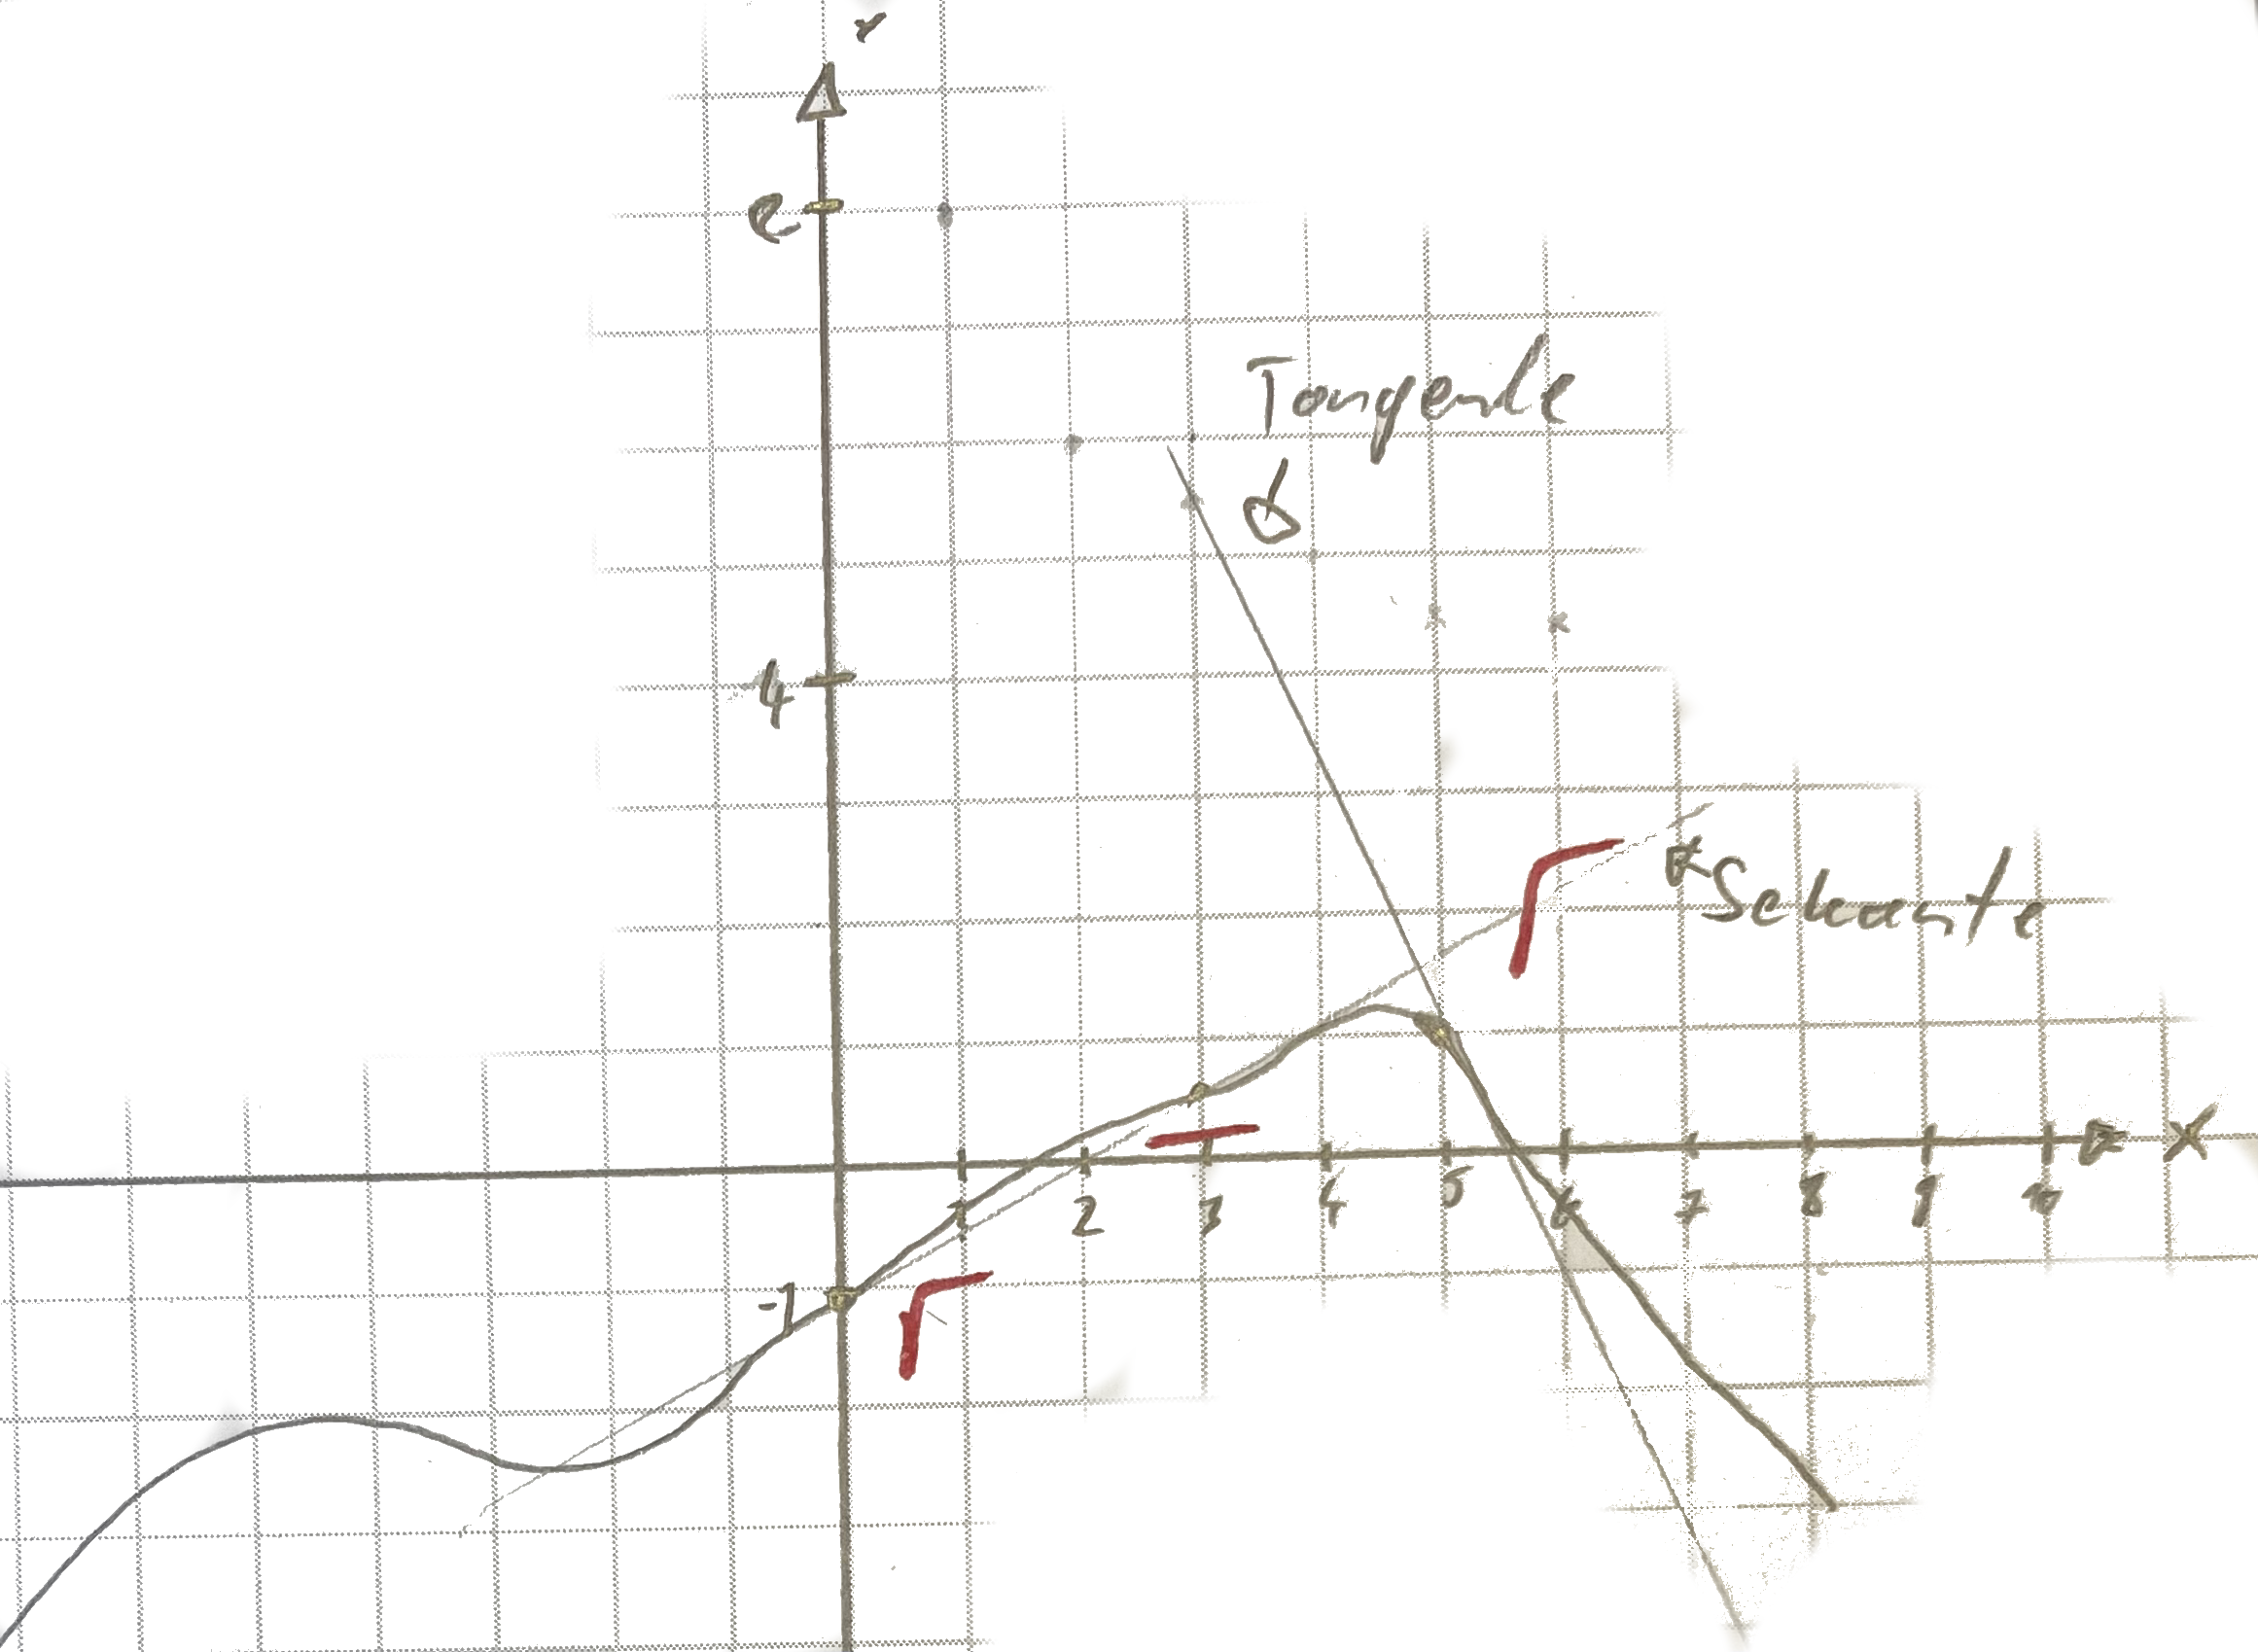
\includegraphics[width=0.4\textwidth]{math-figures/ka-1-3a.png}
    \caption{Ungenau aber richtig}
\end{figure}
\subsection*{Taschenrechner Teil}
\textbf{Aufgabe 1.1}
Hier stelle man sich den Plot $f(x)=(x-2)^3+1$ vor weil pgfplots keine lust hat.

\noindent \textbf{Aufgabe 1.2} $x \in ]-\infty-\infty[$\\
\noindent \textbf{Aufgabe 1.3}
\begin{align*}
   y&= (x-2)^3+1 \\ 
   y-1&= (x-2)^3 \\
   \sqrt[3]{y-1}&= x-2 \\ 
   x&=\sqrt[3]{y-1}+2 \\
   \to f^{-1}(x)&= \sqrt[3]{x-1}+2\\
\end{align*}
\textbf{Aufgabe 1.4} $\mathbb{D}=\mathbb{R}$; Wertebereich: $(-\infty;+\infty)$\\
\textbf{Aufgabe 2.1} 
A: Weiterer Extrempunkt für g ist (-2,-1) und für f ist es (-2,1).

\noindent\textbf{Aufgabe 2.2}
\[x(-x)=f(-x)\cdot (g(-x))^3=f(x)\cdot (-g(x))^3=-f(x)(g(x))^3=-h(x)\]
$\implies$ h ist symmetrisch bzgl. des Koordinatenursprungs
\clearpage% }}}

% h methode{{{
\section{``h-Methode''}
\subsection{Unterricht}
\textbf{Buch Seite 72, Aufgabe 10}
Gegeben ist die Funktion $f$ mit $f(x)=2^x$. Zeigen Sie, dass für jede reelle Zahl $x_0$ der Differenzquotient von f im Intervall $[x_0; x_0+2]$ mit $\frac{3}{2}\cdot f(x_0)$ übereinstimmt. 
\begin{align*}
    f'(x) &= \lim_{h \to 0}\frac{f(x_0+h)-f(x_0)}{h} \\
          &= \lim_{h \to 0}\frac{2^{x_0+h}-2^{x_0}}{h} \\
          &= \lim_{h \to 0}\frac{2^{x_0}\cdot 2^h-2^{x_0}}{h} \\
          &= \lim_{h \to 0}\frac{2^{x_0}\cdot (2^h-1)}{h} \\
          &= 2^{x_0}\cdot \lim_{h \to 0}\frac{2^h-1}{h}=f(x_0)\cdot \lim_{h \to 0}\frac{2^h-1}{h} \\
\end{align*}
% }}}

% die Ableitungsfunktion{{{
\section{Unterricht 06.02.2023}
\subsection{Die Ableitungsfunktion}
\textbf{Beispiel:}$f(x)=x^2$\\
Ableitung an der stelle $x_0=3$
\begin{align*}
  f'(x) &= \lim_{x \to 3}\frac{f(x)-f(3)}{x-3}\\
&= \lim_{x \to 3}\frac{x^2-3^2}{x-3}\\
&=\lim_{x \to 3}\frac{(x-3)(x+3)}{x-3}\\
&=\lim_{x\to3} \frac{\cancel{(x-3)}(x+3)}{\cancel{x-3}}\\
&=3+3=6\\
\end{align*}

\noindent\textbf{Ableitung an einer beliebigen Stelle $x_0$.}\\
\begin{align*}
  f'(x_0)&=\lim_{x\to 0}\frac{f(x)-f(x_0)}{x-x_0}\\
  &= \lim_{x\to 0}\frac{x^2-x_0^2}{x-x_0}\\
  &=\lim_{x\to x_0}\frac{1\cancel{(x-x_0)}(x+x_0)}{1\cancel{x-x_0}}\\
  &=x_0+x_0=2x_0\\
\end{align*}
Das ist dann die Ableitungsfunktion

\noindent\textbf{Aufgabe}
Die Funktion $x \to f'(x)$, die jedem x aus der Definitionsmenge von f die
Ableitung f'(x) an der Stelle x zuordnet, heißt \textbf{Ableitungsfunktion f'}
oder \textbf{Ableitung von f.} Der Wert f'(x) gibt die Steigung des Graphen
$K_f$ im Punkt P(x|f(x)) bzw. die Steigung der Tangente an $K_f$ an dieser
Stelle an.\\

\noindent \textbf{Weitere Beispiele:} $f(x)=1; f(x)=x; f(x)=x^3$.\\
Ableitung von $f(x)=1$ ist 0, Ableitung von $f(x)=x$ ist 1, Ableitung von
$f(x)=x^3$ ist $3x^2$.\\
Nebenrechnung für $f(x)=x^3$\\

\begin{align*}
f'(x_0) &= \lim_{x\to x_0}\frac{f(x)-f(x_0)}{x-x_0} \\ 
        &=\lim_{x\to x_0}\frac{x^3-x_0^3}{x-x_0}\\
        &=\lim_{x \to 0}(x^2+x_0\cdot x+x_0^2)\\
        &=x_0^2+x_0\cdot x_0+x_0^2\\
        &=3x_0^2\\
\end{align*}

\nt{Nebennebenrechnung (soll eine Polynomdivision darstellen):\\
\begin{align*}
  (x^3-x_0^3):(x-x_0)&=x^2+x_0\cdot x\cdot x_0^2\\
  -f(x^3-x_0\cdot x^2) \\
  -----\\
  x_0\cdot x^2-x_0^3 \\
  -(x_0\cdot x^2-x_0^2\cdot x)\\
  ----\\
  x_0^2\cdot x-x_0^3 \\ 
  -(x_0^2\cdot x-x_0^3)\\
  ---\\
  0
\end{align*} }

\begin{table}[h]
  \label{tab:tablee-abl}
  \begin{center}
    \begin{tabular}[c]{l|l}
      \hline
      \multicolumn{1}{r|}{\textbf{f(x)}} & 
      \multicolumn{1}{l}{\textbf{f'(x)}} \\
      1 & 0 \\
      x & 1 \\
      $x^2$ & $2\cdot x$ \\
      $x^3$ & $3\cdot x^2$ \\
      $x^n$ & $n\cdot x^{n-1}$ \\
    \end{tabular}
  \end{center}
  \caption{Herleitung zur Kettenregel}
\end{table}

%\begin{figure}[htpb]
  %\centering
    %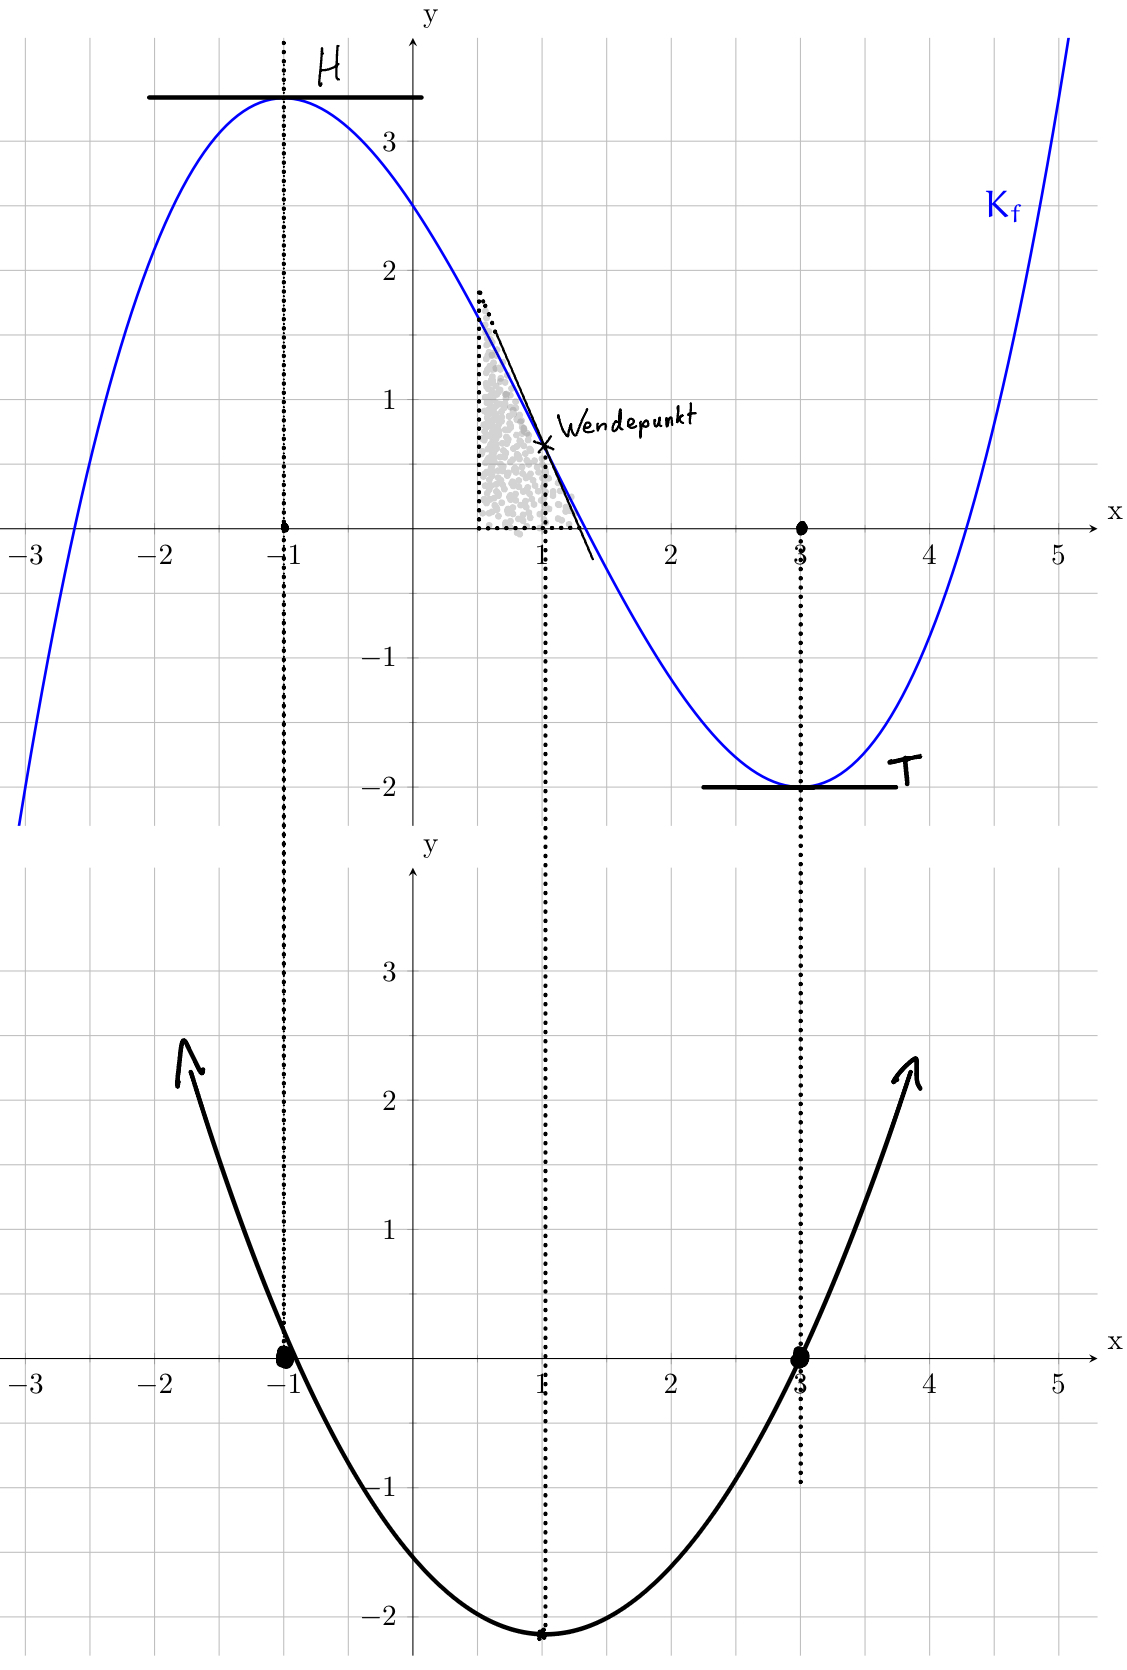
\includegraphics[width=.25\textwidth]{/math-figures/grafische-abl-1.jpeg}
  %\caption{Grafisches Ableiten}
  %\label{fig:graf-abl-1}
%\end{figure}


%\subsection{Hausaufgaben}
%\begin{minipage}{\textwidth}
  %\begin{center}
    %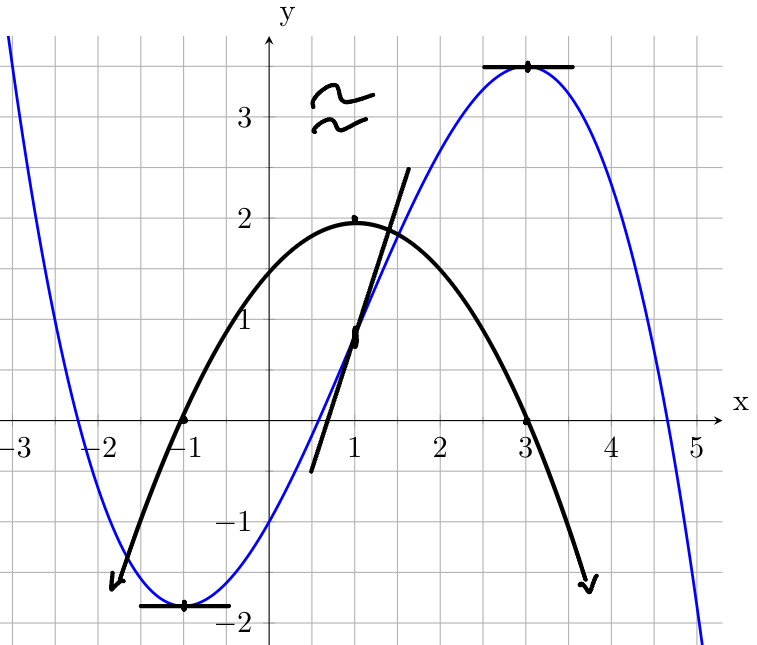
\includegraphics[width=.4\textwidth]{/math-figures/grafische-abl-2.jpeg}
    %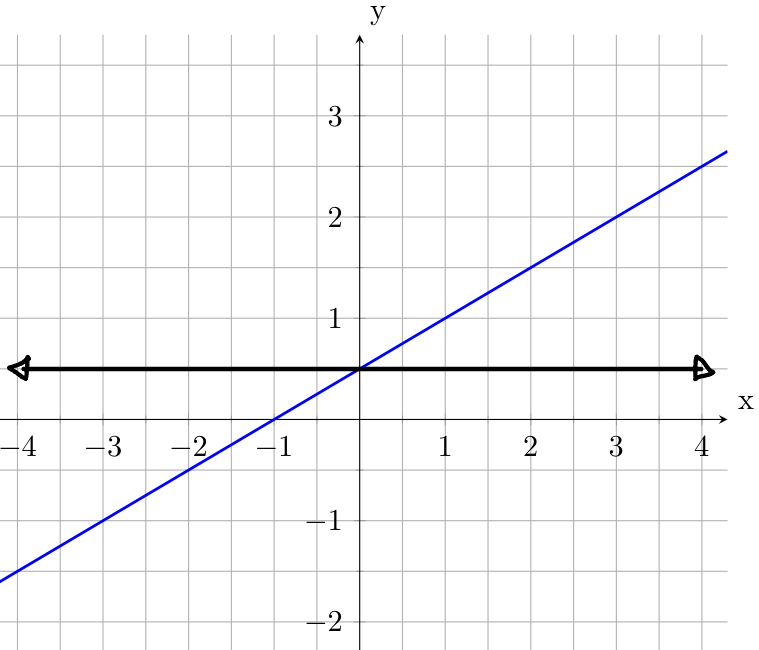
\includegraphics[width=.4\textwidth]{/math-figures/grafische-abl-2-5.jpeg}
  %\end{center} 
%\end{minipage}

%\begin{minipage}{\textwidth}
  %\begin{center}
    %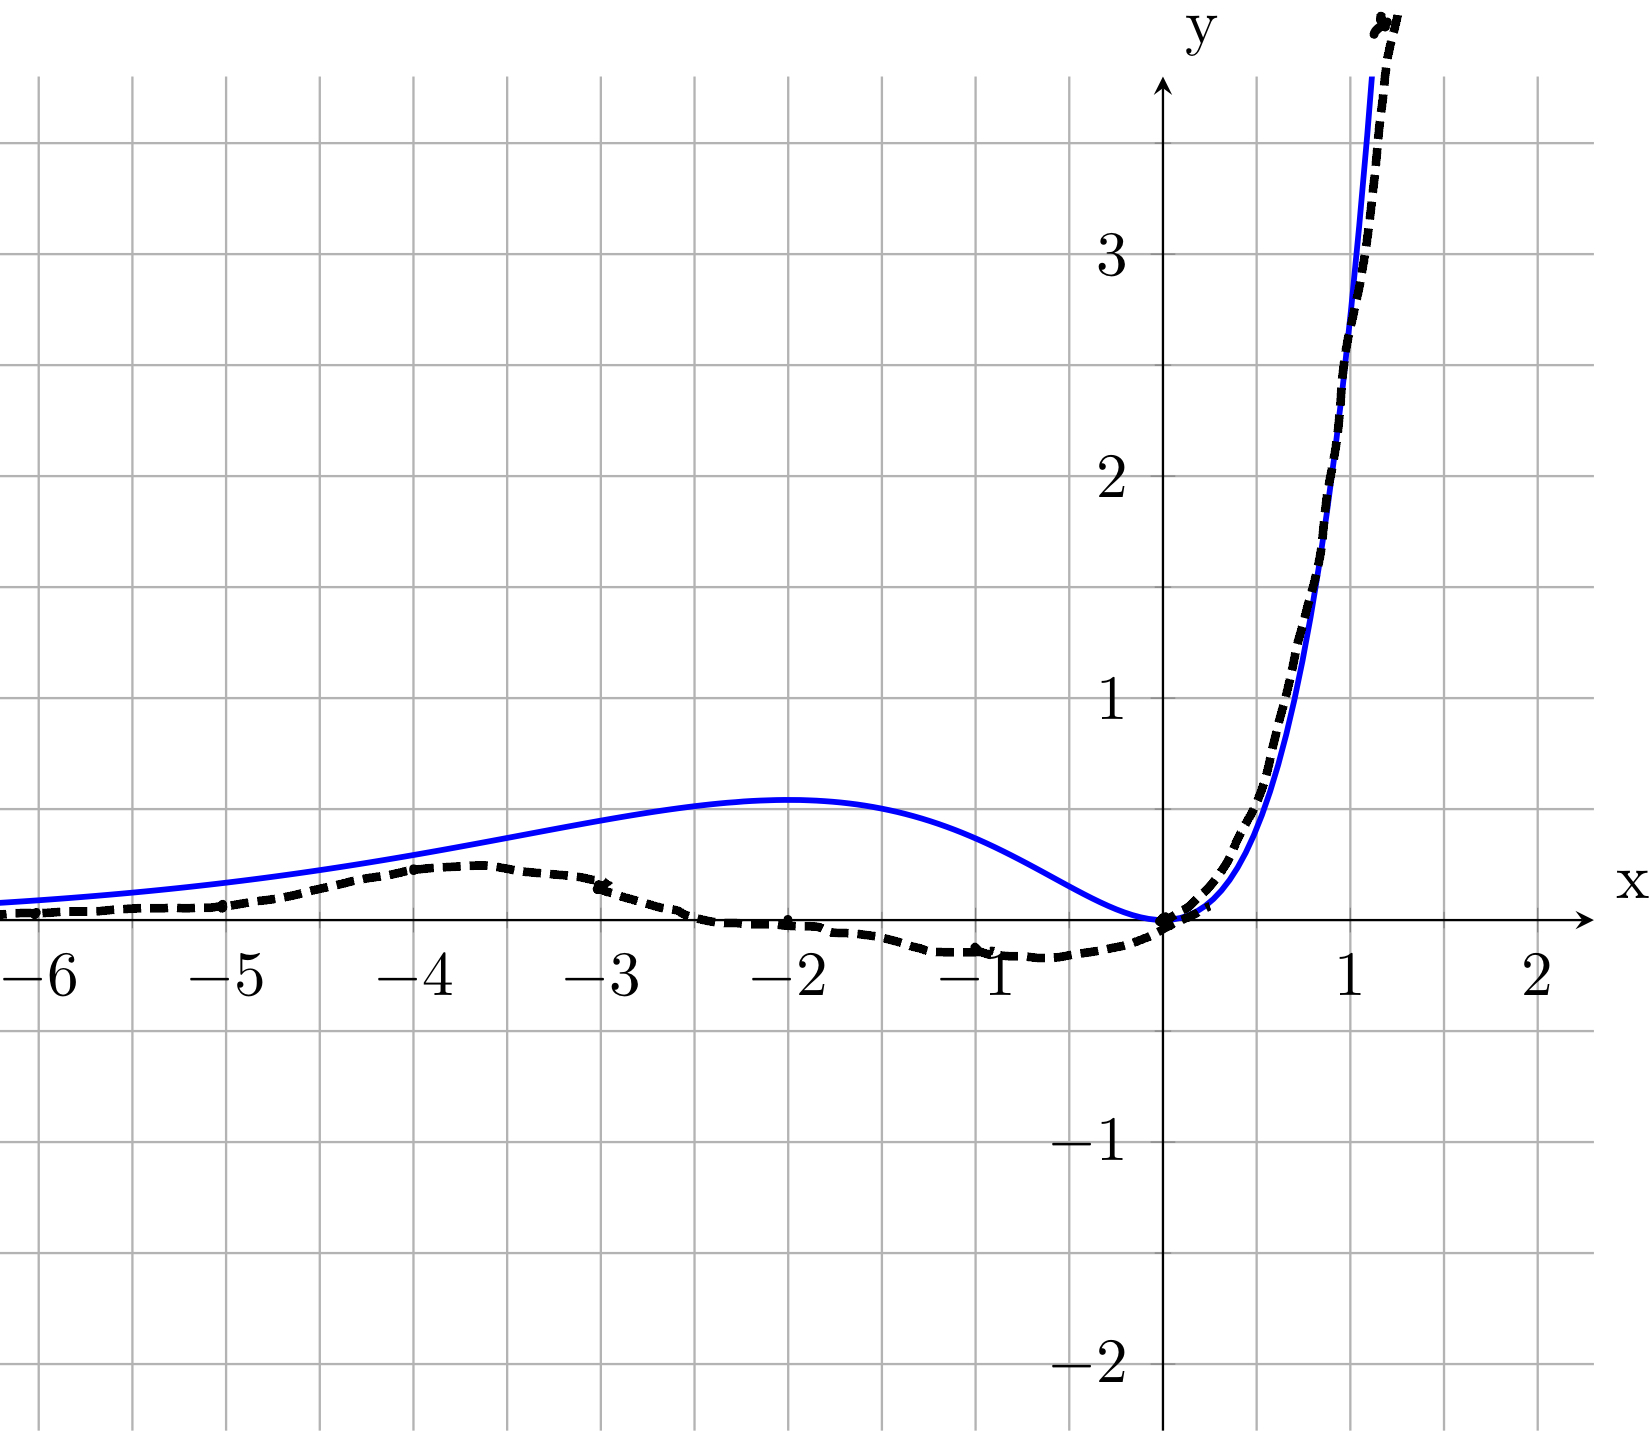
\includegraphics[width=.4\textwidth]{/math-figures/grafische-abl3.jpeg}
    %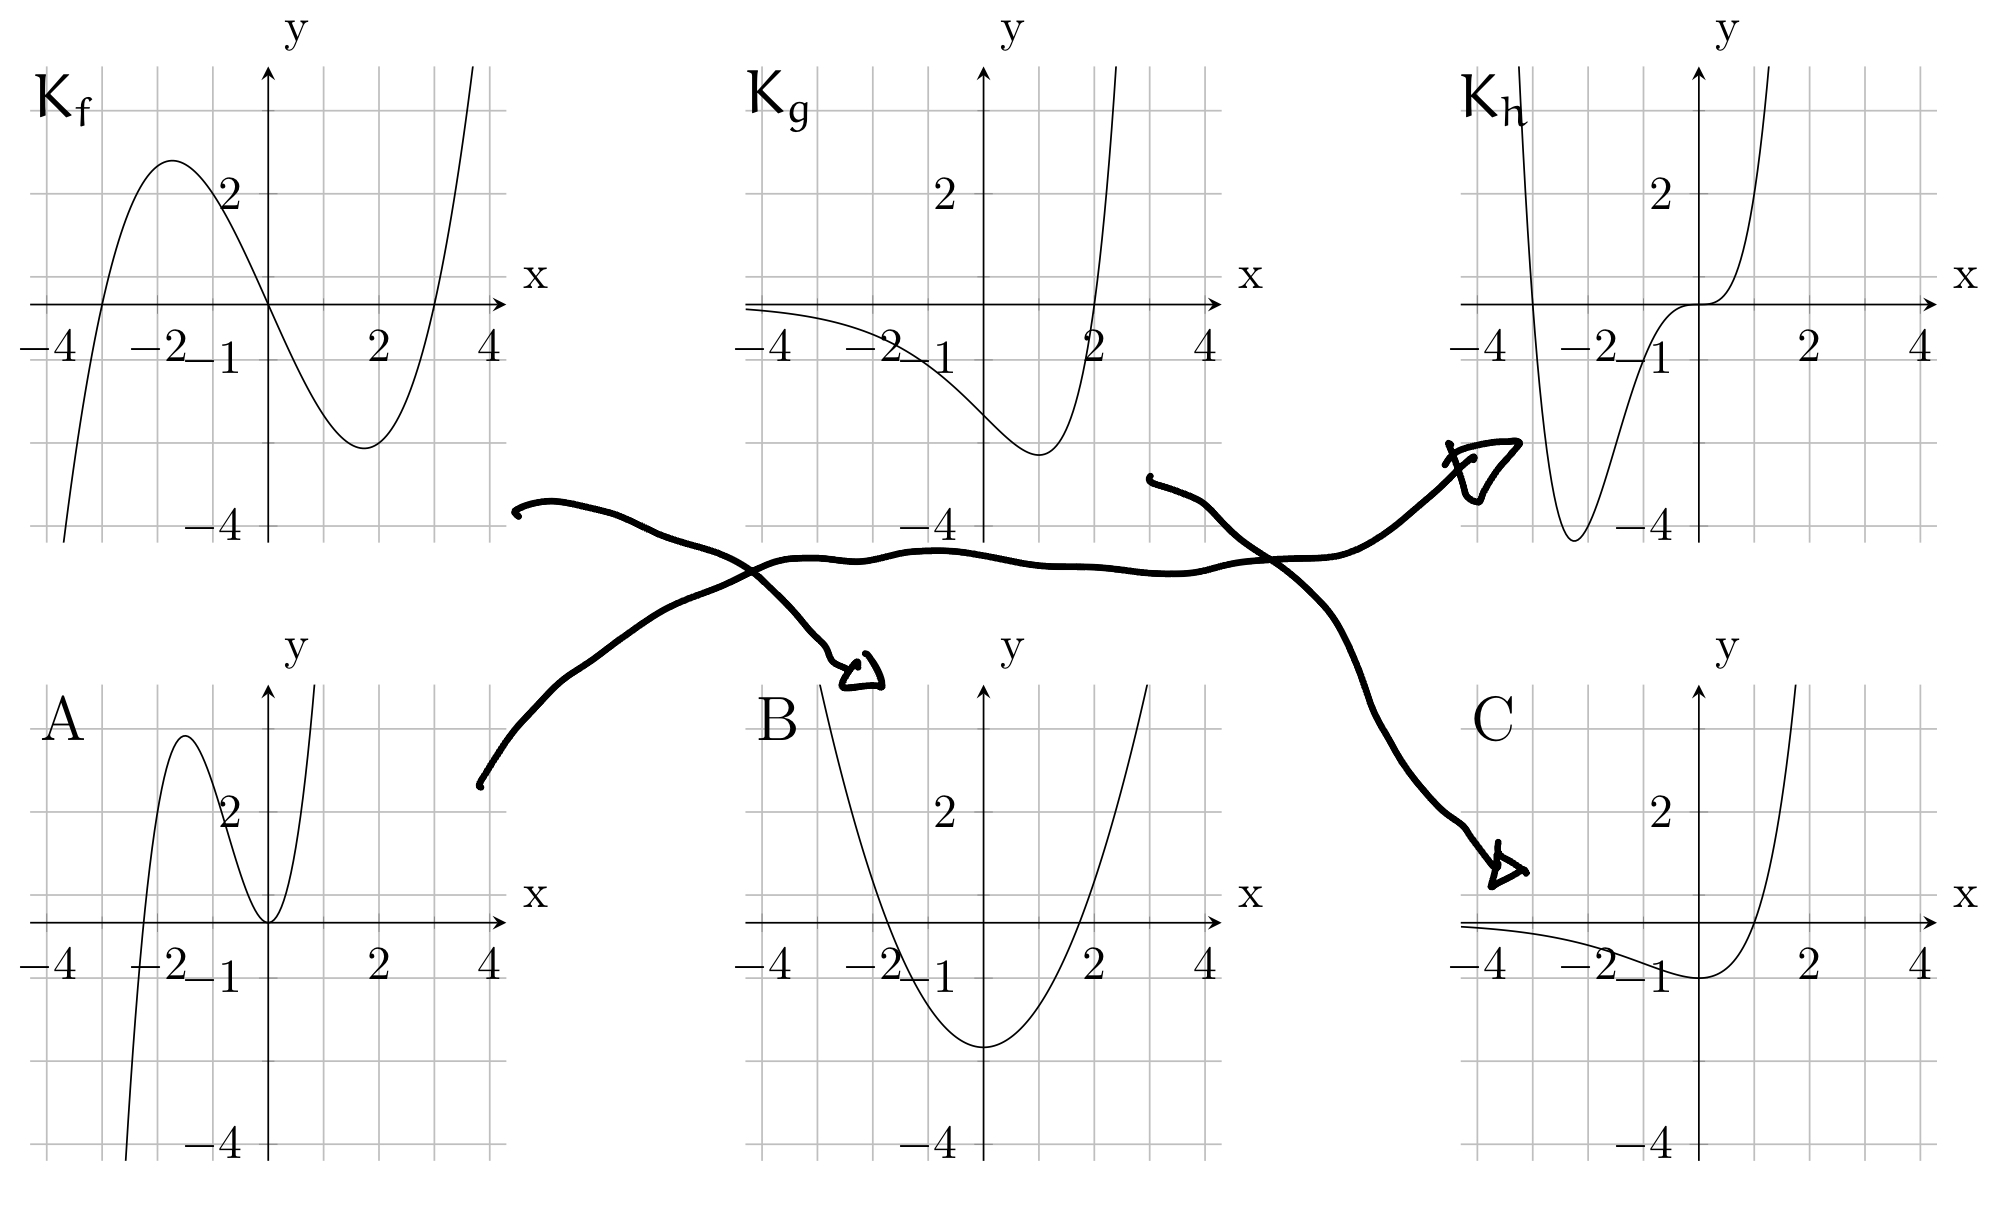
\includegraphics[width=.5\textwidth]{/math-figures/grafische-abl4.jpeg}
  %\end{center} 
%\end{minipage}

Ausrichtung von oben links im Uhrzeigersinn: 1a, 1c, 2, 1b.
Begründung aufgabe 2
$K_f\implies B$ weil bei $K_f$'s äußeren Steigungen sehr steil sind wie bei
einer Parabel in $B$.\\
$K_g\implies C$ weil es übereinstimmt.\\
$K_h\implies A$ weil es übereinstimmt.\\
% }}}

% produktregel und aufgaben{{{
\section{Produktregel, 10.02.2023}
\begin{multicols}{2}
\subsection{Unterricht}
\begin{align*}
  f(x)&=x\cdot x^2 (=x^3)\\
  f(x)&=1\cdot x^2+x\cdot 2x\\
  &=3x^2\\
  &\\
  g(x)&=x^2\cdot e^x\\
  g'(x)&=2\cdot x\cdot e^x+x^2\cdot e^x\\
  &=(2x+x^2)\cdot e^x\\
\end{align*}

\paragraph{Produktregel:}
\begin{equation}
  \frac{df}{dx}\left[f(x)\cdot g(x)\right] = f'(x)\cdot g(x)+f(x)\cdot g'(x)
\end{equation}

\paragraph{ein paar test aufgaben} % (fold)
\label{par:ein paar test aufgaben}
\begin{align*}
  \frac{d}{dx} (x^2 \cdot  x^3) &= \frac{d}{dx}\left[x^2\right]\cdot x^3+x^2\cdot \frac{d}{dx}\left[x^3\right]\\
                           &= 2x\cdot x^3 + x^2 \cdot 3x^2\\
                           &= 2x^4+3x^4\\
                           &= 5x^4
\end{align*}
\begin{align*}
  \frac{d}{dx} (x^3 \cdot  e^x) &=\frac{d}{dx}\left[x^3\right] \cdot e^x + x^3 \cdot \frac{d}{dx}\left[e^x\right]\\
  &=3x^2 \cdot e^x + x^3 \cdot e^x \\
\end{align*}
\begin{align*}
  \frac{d}{dx} (x \cdot  \sin(x)) &=\frac{d}{dx}\left[x\right]\cdot \sin(x) + x \cdot \frac{d}{dx}\left[\sin(x)\right]\\
  &=1 \cdot \sin(x) + x \cdot \cos(x)\\
  &=\sin(x)+x\cos(x)\\                           
\end{align*}
\begin{align*}
\frac{d}{dx} (e^x \cdot  cos(x)) &=e^x \cdot \cos(x)+ e^x \cdot -\cos(x) \\
\end{align*}

\begin{align*}
\frac{d}{dx} (x^2 \cdot  ln(x)) &=2x \cdot \ln(x) + x^2 \cdot \frac{1}{x}\\
&=2x \ln(x) + x\\
\end{align*}
\paragraph{bisschen schwerere} % (fold)
\label{par:bisschen schwerere}

\begin{align*}
&\frac{d}{dx} (x^4 \cdot sin(x^2)) =\\
&=4x^3\cdot\sin(x^2)+x^4 \cdot \frac{d}{dx}\left[\sin(x^2)\right] \\
&=4x^3\cdot\sin(x^2)+x^4 \cdot \frac{df}{du}\left[\sin(u)\right] \cdot \frac{du}{dx}\left[x^2\right] \\
&=4x^3\cdot\sin(x^2)+x^4 \cdot \cos(x^2)\cdot 2x\\
&=4x^3 \cdot sin(x^2)+2x^5 \cdot \cos(x^2)\\
\end{align*}

\begin{align*}
\frac{d}{dx} (e^{2x} \cdot x^3) &=2e^{2x} \cdot x^3 + e^{2x} \cdot 3x^2 \\
                                &=3e^{2x} \cdot x^3 + 3x^2\\
\end{align*}
\begin{align*}
\frac{d}{dx} (x^2 \cdot  e^{x^2}) &=2x \cdot e^{x^2} + x^2 \cdot 2e^x\\
\end{align*}
\begin{align*}
\frac{d}{dx} (x \cdot  ln(x^3)) &=1 \cdot ln(x^3) + x \frac{3}{x}\\
\end{align*}
\begin{align*}
\frac{d}{dx} (e^x \cdot  \sin(x^3)) &=e^x \cdot \sin(x^3) + e^x \cdot \cos(x^3) \cdot 3x^2 \\
&=2e^x \cdot sin(x^3) + \cos(x^3) \cdot 3x^2\\
\end{align*}
\end{multicols}
\begin{multicols}{2}[Schulbuch Aufgaben, Seite 79, Nr. 1-4]
\paragraph{Aufgabe 1} % (fold)
\label{par:Aufgabe 1}
\begin{align*}
\frac{d}{dx}\left[3x^2\right]&=6x\\
\frac{d}{dx}\left[-7x^4\right]&=-28x^3\\
\frac{d}{dx}\left[5x\right]&=5\\
\frac{d}{dx}\left[-\frac{1}{5}x^{10}\right]&=-2x^9\\
\frac{d}{dx}\left[\frac{4}{x}\right]&=\frac{4}{x^2}\\
\frac{d}{dx}\left[-\frac{2}{5}x^{-5}\right]&=-x^{-6}\\
\frac{d}{dx}\left[4\sqrt{x}\right]&=\frac{2}{\sqrt{x}}\\
\end{align*}

\paragraph{Aufgabe 2} % (fold)
\label{par:Aufgabe 2}
\begin{align*}
\frac{d}{dx}\left[2x^3+5x^2\right]&=6x^2+10x\\
\frac{d}{dx}\left[4x^5-3x\right]&=20x^4-3\\
\frac{d}{dx}\left[2x^7-3x^4\right]&=14x^6-12x^3\\
\frac{d}{dx}\left[-2x^3+x^2+4\right]&=-6x^2+2x\\
\frac{d}{dx}\left[2x^3(x^2+x-1)\right]&=6x^2 \cdot 3x + (x^2+x-1) \cdot 2x^3\\
\frac{d}{du}\left[u(u+3)^2\right]&=?\text{zu verkettet}?\\
\end{align*}
% paragraph paragraph name (end)

\paragraph{Aufgabe 3 (f'(x)-f'''(x))} % (fold)
\label{par:Aufgabe 3}
\begin{align*}
f(x)&=-\frac{3}{2}x^2+\frac{5}{4}x+2\\
f'(x)&=-2x+...\\
\end{align*}
% paragraph paragraph name (end)

\paragraph{Aufgabe 4} % (fold)
\label{par:aufgabe-vier}
\text{Steigung rausfinden an Punkt A(2|f(2))}\\
\begin{align*}
\frac{d}{dx}\left[\frac{3}{2}x^2\right]&=2x\\
2\cdot 2 &= 4\\
    &=\text{m=4}\\
\end{align*}
\begin{align*}
 \frac{d}{dx}\left[\frac{1}{4}t^4-\frac{5}{3}t^3\right]&=t^3-5t^2\\
 &=2^2-5\cdot 2^2\\
 &=4-20\\
 &=m=-16\\
\end{align*}
\begin{align*}
  \frac{d}{dz}\left[\frac{3}{4}z^2-3x^{-1}\right] &= 1,5z+3z^{-2}\\
  &=m=3,75\\
\end{align*}
\begin{align*}
 \frac{d}{dx}\left[-x-2x^4\right] &=-1+8x\\
 &=m=15\\
\end{align*}
\paragraph{Aufgabe 10} 
\label{par:Aufgabe 10}
\begin{align*}
\frac{d}{dx}\left[e^{\sin(2x)}\right]&=\\
&=\frac{du}{dx}\left[e^x\right]\frac{df}{du}\left[\sin(2x)\right]\\
&=e^{\sin(2x)}*2\cos(2x)\\
\end{align*}

\end{multicols}
\paragraph{kubische Formel}
\label{par:kubische Formel}
\[x = \sqrt[3]{\frac{q + \sqrt{q^2 + \frac{4p^3}{27}}}{2}} - \sqrt[3]{\frac{-q + \sqrt{q^2 + \frac{4p^3}{27}}}{2}} - \frac{b}{3a}\]
wobei $p = \frac{3ac - b^2}{3a^2}$ und $q = \frac{2b^3 - 9abc + 27a^2d}{27a^3}$.
Wenn man zuviel zeit hat könnte man damit folgendes ausrechnen:\\
$x^3-7x^2+15x-9$.
\begin{align*}
p &= \frac{3ac - b^2}{3a^2} = \frac{3 \cdot 1 \cdot 15 - 7^2}{3 \cdot 1^2} = \frac{6}{3} = 2 \\
q &= \frac{2b^3 - 9abc + 27a^2d}{27a^3} = \frac{2 \cdot 7^3 - 9 \cdot 1 \cdot 7 \cdot 15 + 27 \cdot 1^2 \cdot 9}{27 \cdot 1^3} = \frac{-27}{27} = -1 \\
\alpha &= \sqrt[3]{\frac{q + \sqrt{q^2 + \frac{4p^3}{27}}}{2}} = \sqrt[3]{\frac{-1 + \sqrt{1 + \frac{32}{27}}}{2}} \approx 1.5 \\
\beta &= \sqrt[3]{\frac{-q + \sqrt{q^2 + \frac{4p^3}{27}}}{2}} = \sqrt[3]{\frac{1 + \sqrt{1 + \frac{32}{27}}}{2}} \approx 1.5 \\
\gamma &= -\frac{b}{3a} = -\frac{7}{3}
\end{align*}

Daher sind die Nullstellen von $x^3 - 7x^2 + 15x - 9$ gegeben durch:

\begin{align*}
x_1 &= \alpha + \beta + \gamma \approx 4 \\
x_2 &= -\frac{\alpha + \beta}{2} + \frac{\sqrt{3}}{2}i(\alpha - \beta) + \gamma \approx 1 \\
x_3 &= -\frac{\alpha + \beta}{2} - \frac{\sqrt{3}}{2}i(\alpha - \beta) + \gamma \approx 1 \\
\end{align*}
\begin{align*}
p &= \frac{3ac - b^2}{3a^2} = \frac{3 \cdot 1 \cdot 15 - 7^2}{3 \cdot 1^2} = \frac{6}{3} = 2 \\
q &= \frac{2b^3 - 9abc + 27a^2d}{27a^3} = \frac{2 \cdot 7^3 - 9 \cdot 1 \cdot 7 \cdot 15 + 27 \cdot 1^2 \cdot 9}{27 \cdot 1^3} = \frac{-27}{27} = -1 \\
\alpha &= \sqrt[3]{\frac{q + \sqrt{q^2 + \frac{4p^3}{27}}}{2}} = \sqrt[3]{\frac{-1 + \sqrt{1 + \frac{32}{27}}}{2}} \approx 1.5 \\
\beta &= \sqrt[3]{\frac{-q + \sqrt{q^2 + \frac{4p^3}{27}}}{2}}
\end{align*}

% Winterferien {{{
\clearpage
\section{Winterferien}
\subsubsection{csc, sec and cot} % (fold)
\label{ssub:csc-sec-and-cot}
The cosecant, secant, and cotangent functions are defined as follows:

$$\csc(\theta) = \frac{1}{\sin(\theta)}$$

$$\sec(\theta) = \frac{1}{\cos(\theta)}$$

$$\cot(\theta) = \frac{1}{\tan(\theta)} = \frac{\cos(\theta)}{\sin(\theta)}$$

where $\theta$ is an angle measured in radians or degrees.

The cosecant of an angle $\theta$ is defined as the reciprocal of the sine of
$\theta$. That is, if $x$ is the length of the side opposite to $\theta$ and
$h$ is the length of the hypotenuse of a right triangle that contains $\theta$,
then:

$$\csc(\theta) = \frac{h}{x}$$

The secant of an angle $\theta$ is defined as the reciprocal of the cosine of
$\theta$. That is, if $y$ is the length of the side adjacent to $\theta$ and
$h$ is the length of the hypotenuse of a right triangle that contains $\theta$,
then:

$$\sec(\theta) = \frac{h}{y}$$

The cotangent of an angle $\theta$ is defined as the reciprocal of the tangent
of $\theta$. That is, if $x$ is the length of the side adjacent to $\theta$ and
$y$ is the length of the side opposite to $\theta$, then:

$$\cot(\theta) = \frac{x}{y}$$

\paragraph{does this mean they are basically the same as} $\sin^{-1}$, $\cos^{-1}$ and $\tan^{-1}$\textbf{?}
No, the cosecant, secant, and cotangent functions are not the same as the
inverse trigonometric functions, which are commonly denoted as $\sin^{-1}$,
$\cos^{-1}$, and $\tan^{-1}$.

The inverse trigonometric functions are used to find the angle that produces a
given ratio of sides in a right triangle. For example, if we know the length of
two sides of a right triangle, we can use the inverse trigonometric functions
to find the measure of the angle opposite to the known sides. The output of an
inverse trigonometric function is an angle, whereas the output of the cosecant,
secant, and cotangent functions is a ratio of sides.

The inverse trigonometric functions are defined as follows:

$$\sin^{-1}(x) = \theta \qquad \text{if} \qquad \sin(\theta) = x \qquad \text{and} \qquad -\frac{\pi}{2} \leq \theta \leq \frac{\pi}{2}$$

$$\cos^{-1}(x) = \theta \qquad \text{if} \qquad \cos(\theta) = x \qquad \text{and} \qquad 0 \leq \theta \leq \pi$$

$$\tan^{-1}(x) = \theta \qquad \text{if} \qquad \tan(\theta) = x \qquad \text{and} \qquad -\frac{\pi}{2} < \theta < \frac{\pi}{2}$$

Note that the inverse trigonometric functions are also commonly denoted as
$\arcsin$, $\arccos$, and $\arctan$.

In summary, the cosecant, secant, and cotangent functions are reciprocals of
the sine, cosine, and tangent functions, respectively, and are used to find the
ratios of sides in a right triangle. The inverse trigonometric functions, on
the other hand, are used to find the angles that produce a given ratio of sides
in a right triangle.



\paragraph{Ableitungen} % (fold)
\label{par:Ableitungen}
To take the derivatives of the cosecant, secant, and cotangent functions, we
can use the quotient rule of differentiation along with the chain rule. Here
are the formulas for finding the derivatives:

$$\frac{d}{dx} \csc(x) = -\csc(x) \cot(x)$$

$$\frac{d}{dx} \sec(x) = \sec(x) \tan(x)$$

$$\frac{d}{dx} \cot(x) = -\csc^2(x)$$

where $x$ is the independent variable (usually an angle) with respect to which
we are differentiating.

To derive these formulas, we start with the definitions of the cosecant,
secant, and cotangent functions in terms of the sine, cosine, and tangent
functions:

$$\csc(x) = \frac{1}{\sin(x)}$$

$$\sec(x) = \frac{1}{\cos(x)}$$

$$\cot(x) = \frac{1}{\tan(x)} = \frac{\cos(x)}{\sin(x)}$$

Then, we use the quotient rule of differentiation:

$$\left(\frac{f}{g}\right)' = \frac{f'g - fg'}{g^2}$$

where $f$ and $g$ are functions and $f'$ and $g'$ are their derivatives.

Applying the quotient rule and simplifying, we get:

$$\frac{d}{dx} \csc(x) = -\frac{\cos(x)}{\sin^2(x)} = -\csc(x) \cot(x)$$

$$\frac{d}{dx} \sec(x) = \frac{\sin(x)}{\cos^2(x)} = \sec(x) \tan(x)$$

$$\frac{d}{dx} \cot(x) = -\frac{\cos(x)}{\sin^2(x)} = -\csc^2(x)$$

Therefore, the derivative of the cosecant function is equal to minus the
cosecant function times the cotangent function, the derivative of the secant
function is equal to the secant function times the tangent function, and the
derivative of the cotangent function is equal to minus the cosecant squared
function.

$$\displaystyle\sum_{n}^{\infty}$$
\[\displaystyle\int_{\pi}^{2\pi}\tan x\]
% }}}

\subsection{paar aufgben}
\section{5a}
Bestimmung der Extrempunkte der Funktion $f(x) = x^3 + \frac{3}{2}x^2 - 6x$.

Zunächst müssen wir die erste und zweite Ableitungen der Funktion berechnen:

$$f'(x) = 3x^2 + 3x - 6$$

$$f''(x) = 6x + 3$$

Als nächstes finden wir die Nullstellen von $f'(x)$, indem wir $f'(x) = 0$ setzen und nach $x$ auflösen:

$$3x^2 + 3x - 6 = 0$$

$$x^2 + x - 2 = 0$$

$$(x+2)(x-1) = 0$$

Daraus ergibt sich $x_1=-2$ und $x_2=1$. Diese Werte entsprechen den möglichen Extrempunkten der Funktion.

Nun bestimmen wir die Vorzeichen von $f''(x)$ für die Intervalle $(-\infty,-2)$, $(-2,1)$ und $(1,\infty)$:

$$f''(-3) = -15 < 0$$
$$f''(0) = 3 > 0$$
$$f''(2) = 15 > 0$$

Da $f''(x)$ für $x<-2$ negativ ist, haben wir einen Hochpunkt bei $x=-2$. Da $f''(x)$ für $x>-2$ positiv ist, haben wir ein Minimum bei $x=-2$.

Ähnlich haben wir einen Tiefpunkt bei $x=1$, da $f''(x)$ für $x<1$ positiv und für $x>1$ negativ ist.

Um nun die entsprechenden Funktionswerte zu berechnen, setzen wir $x=-2$ und $x=1$ in die Funktion $f(x)$ ein:

$$f(-2) = (-2)^3 + \frac{3}{2}(-2)^2 - 6(-2) = -8 - 6 + 12 = -2$$

$$f(1) = 1^3 + \frac{3}{2}(1)^2 - 6(1) = 1 + \frac{3}{2} - 6 = -\frac{7}{2}$$

Daher sind die Extrempunkte der Funktion $f(x) = x^3 + \frac{3}{2}x^2 - 6x$ bei $(-2,-2)$ und $(1,-\frac{7}{2})$.

\section*{5b}
Die gegebene Funktion lautet: $f(x) = x^4 e^x$

Um die Extrempunkte der Funktion zu finden, müssen wir zuerst die Ableitungen berechnen:

\begin{align*}
f'(x) &= e^x x^4 + 4 e^x x^3 \\
f''(x) &= e^x x^4 + 8 e^x x^3 + 12 e^x x^2 \\
\end{align*}

Um die kritischen Punkte zu finden, setzen wir die erste Ableitung gleich null und lösen nach $x$ auf:

\begin{align*}
f'(x) &= 0 \\
e^x x^4 + 4 e^x x^3 &= 0 \\
e^x x^3 (x+4) &= 0 \\
\end{align*}

Daraus folgt, dass $x = 0$ oder $x = -4$ oder $f'(x)$ existiert nicht.

Nun überprüfen wir das Vorzeichen der zweiten Ableitung an den kritischen Punkten:

\begin{align*}
f''(0) &= 12 e^0 (0)^2 = 0 \\
f''(-4) &= e^{-4} (-4)^4 + 8 e^{-4} (-4)^3 + 12 e^{-4} (-4)^2 \\
&= e^{-4} (256 - 768 + 576) \\
&= -32e^{-4} < 0 \\
\end{align*}

Da $f''(-4)$ negativ ist, handelt es sich bei $x=-4$ um ein lokales Maximum. Da $f''(0) = 0$ ist, können wir die Art des Punktes bei $x=0$ nicht bestimmen. Wir können jedoch eine zweite Ableitungsprobe durchführen, um zu sehen, ob es sich um ein lokales Maximum oder ein lokales Minimum handelt:

\begin{align*}
f''(1) &= e^1 (1)^4 + 8 e^1 (1)^3 + 12 e^1 (1)^2 \\
&= 21e \\
\end{align*}

Da $f''(1)$ positiv ist, handelt es sich bei $x=0$ um ein lokales Minimum.

Zusammenfassend haben wir:

Der kritische Punkt $x=-4$ ist ein lokales Maximum.
Der kritische Punkt $x=0$ ist ein lokales Minimum.


\textbf{Plot:}

%\begin{tikzpicture}
%\begin{axis}[
    %axis lines = center,
    %xlabel=$x$,
    %ylabel={$f(x)$},
%]
%\addplot [
    %domain=-5:1,
    %samples=100,
    %color=blue,
%]
%{x^4*exp(x)};
%\addlegendentry{$f(x)=x^4e^x$}
%\addplot[
    %mark=*,
    %only marks,
    %color=red,
    %mark options={scale=1.5},
    %nodes near coords,
    %point meta=explicit symbolic,
%]
%coordinates {
    %(-4,768*exp(-4))[lokales Maximum]
    %(0,0)[lokales Minimum]
%%};
%\end{axis}
%\end{tikzpicture}


\begin{tikzpicture}
\begin{axis}[
    xmin=-10, xmax=1.128,
    ymin=0, ymax=10,
    xlabel=$x$,
    ylabel=$f(x)$,
    domain=-10:1.128,
    samples=100
]
\addplot[blue]{x^4*e^x};
%\addplot[dashed] coordinates {(-4, 768) (0,0)};
%\addplot[dashed] coordinates {(0,0) (0, -100)};
\end{axis}
\end{tikzpicture}
clearpage wegen neuer stunde
\clearpage

\section{Mathe Unterricht, 10.03.2023}
Heute machen wir in der einzelnen Stunde glaub nur eine Prüfungsaufgabe
und/oder so, auch ist es im allgmeinfall falsch, dass für Ganzrationale
Funktionen die Extrempunkte immer zwischen ihrenNullstellen sind.

\begin{align*}
f(x)&=x\cdot (x-1)(3-x)\\
&=x\cdot(-x^2+4x-3)\\
&=-x^3+3x^3-3x\\
\implies f'(x)&=-3x^2+8x-3\\
\implies f''(x)&=-6x+8\\
f'(x)=0&\implies -3x^2+8x-3\\
x_{1/2}&=\frac{-8 \pm \sqrt{64-4*(-3)+(-3)}}{-6}\\
       &=\frac{-8\pm \sqrt{28}}{-6}\\
       &=\frac{-8\pm 2\sqrt{7}}{-6}\\
       &x_1= \frac{4}{3}-\frac{1}{3}\sqrt{7}\\
       &x_2=\frac{4}{3}+ \frac{1}{3}\sqrt{7}\\
       &\text{beides sind einfache nullstellen $\implies$ Vorzeichen wechsel}\\
f'(\frac{4}{3})&=-3x^2+8x-3\\
               &=\frac{-16}{3}+\frac{32}{3}-\frac{9}{3}>0\\
f''(\frac{4}{3}-\frac{1}{3}\sqrt{7})&=<0 \implies H\\
\end{align*}
hier wär so ein strahl praktisch, des könnt man evtl. als tikz template machen.


\section{Zusammenfassung für die Arbeit (KA 1, J1-2)}
\subsubsection{Mittere Änderungsrate, x-Methode}
\[\frac{f(x_2)-f(x_1)}{x_2-x_1}\]
Die Änderung gibt an, wie schnell sie die Funktionswerte von $x_1$ nach $x_2$
ändern. Man nennt diesen Quotienten auch \textbf{Differenzquotienten}.

\subsubsection{Änderungsrate, h-Methode}
\[\lim_{x \to x_0}\frac{f(x)-f(x_0)}{x-x_0}\]

\begin{figure}[htpb]
  \begin{center}
    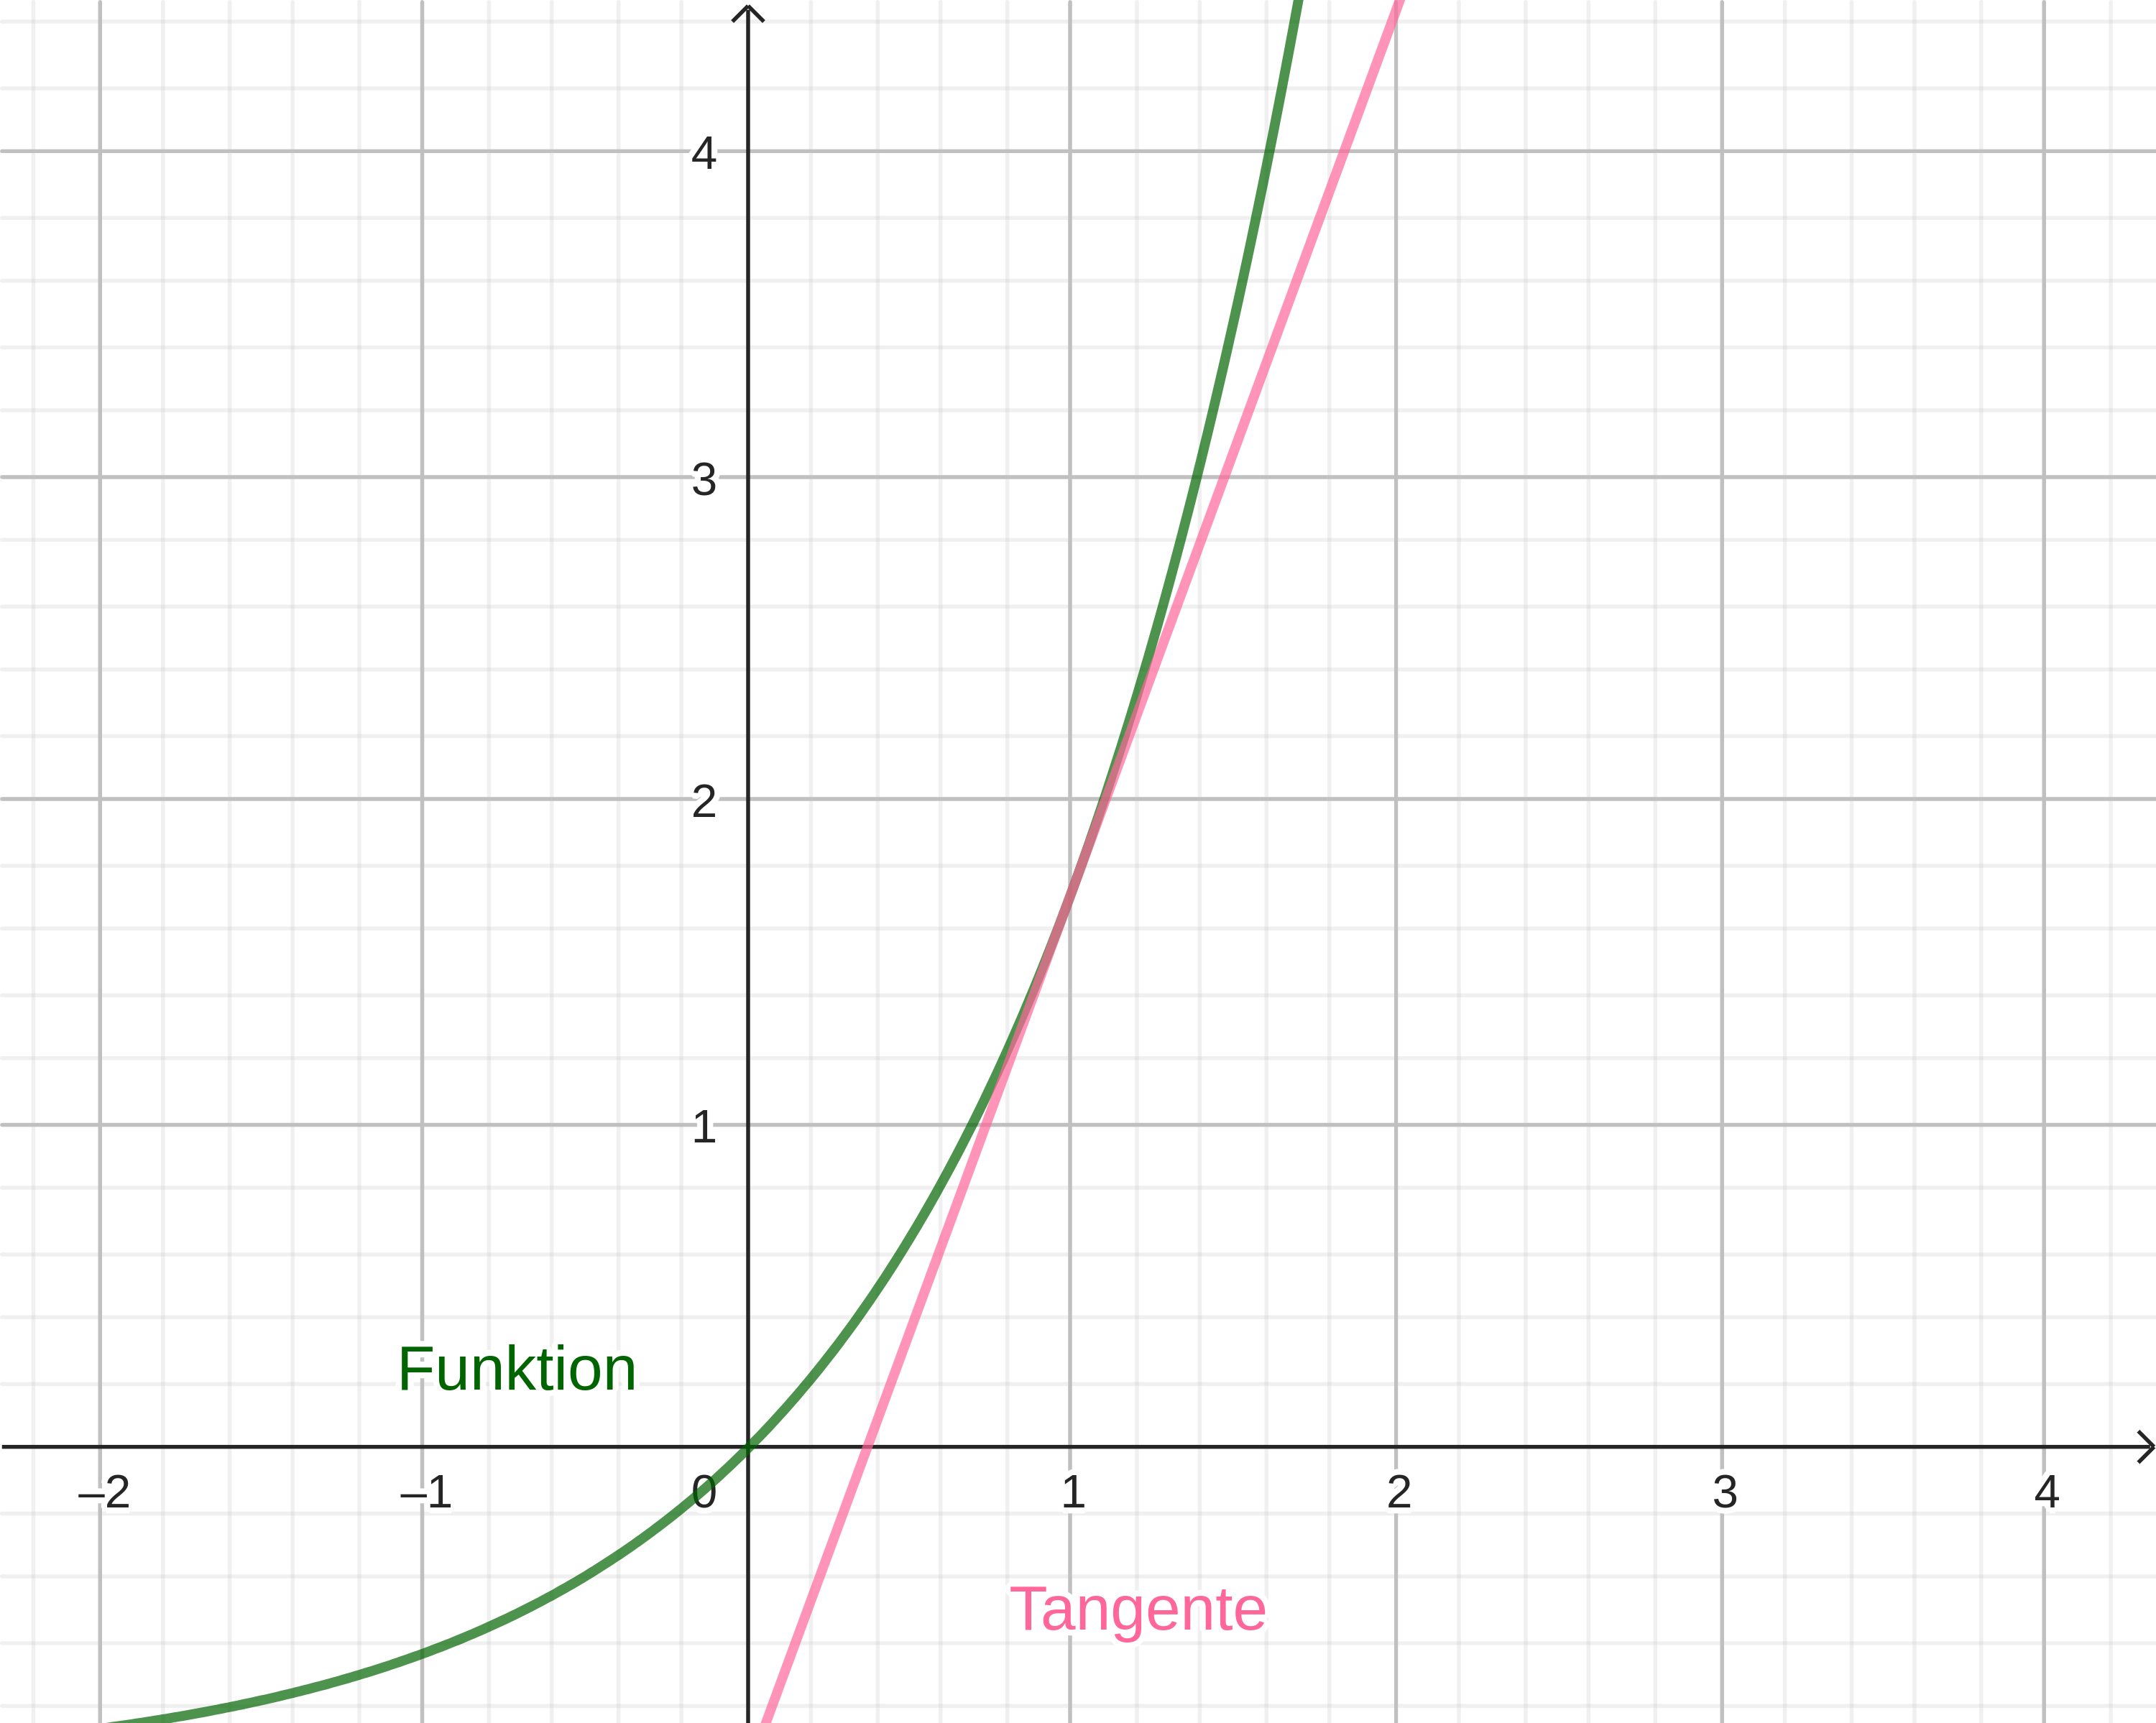
\includegraphics[width=0.15\textwidth]{math-figures/tangente.png}
  \end{center}
  \caption{Eine Tangente grafisch}
\end{figure}

\clearpage

\begin{figure}[htpb]
  \begin{center}
    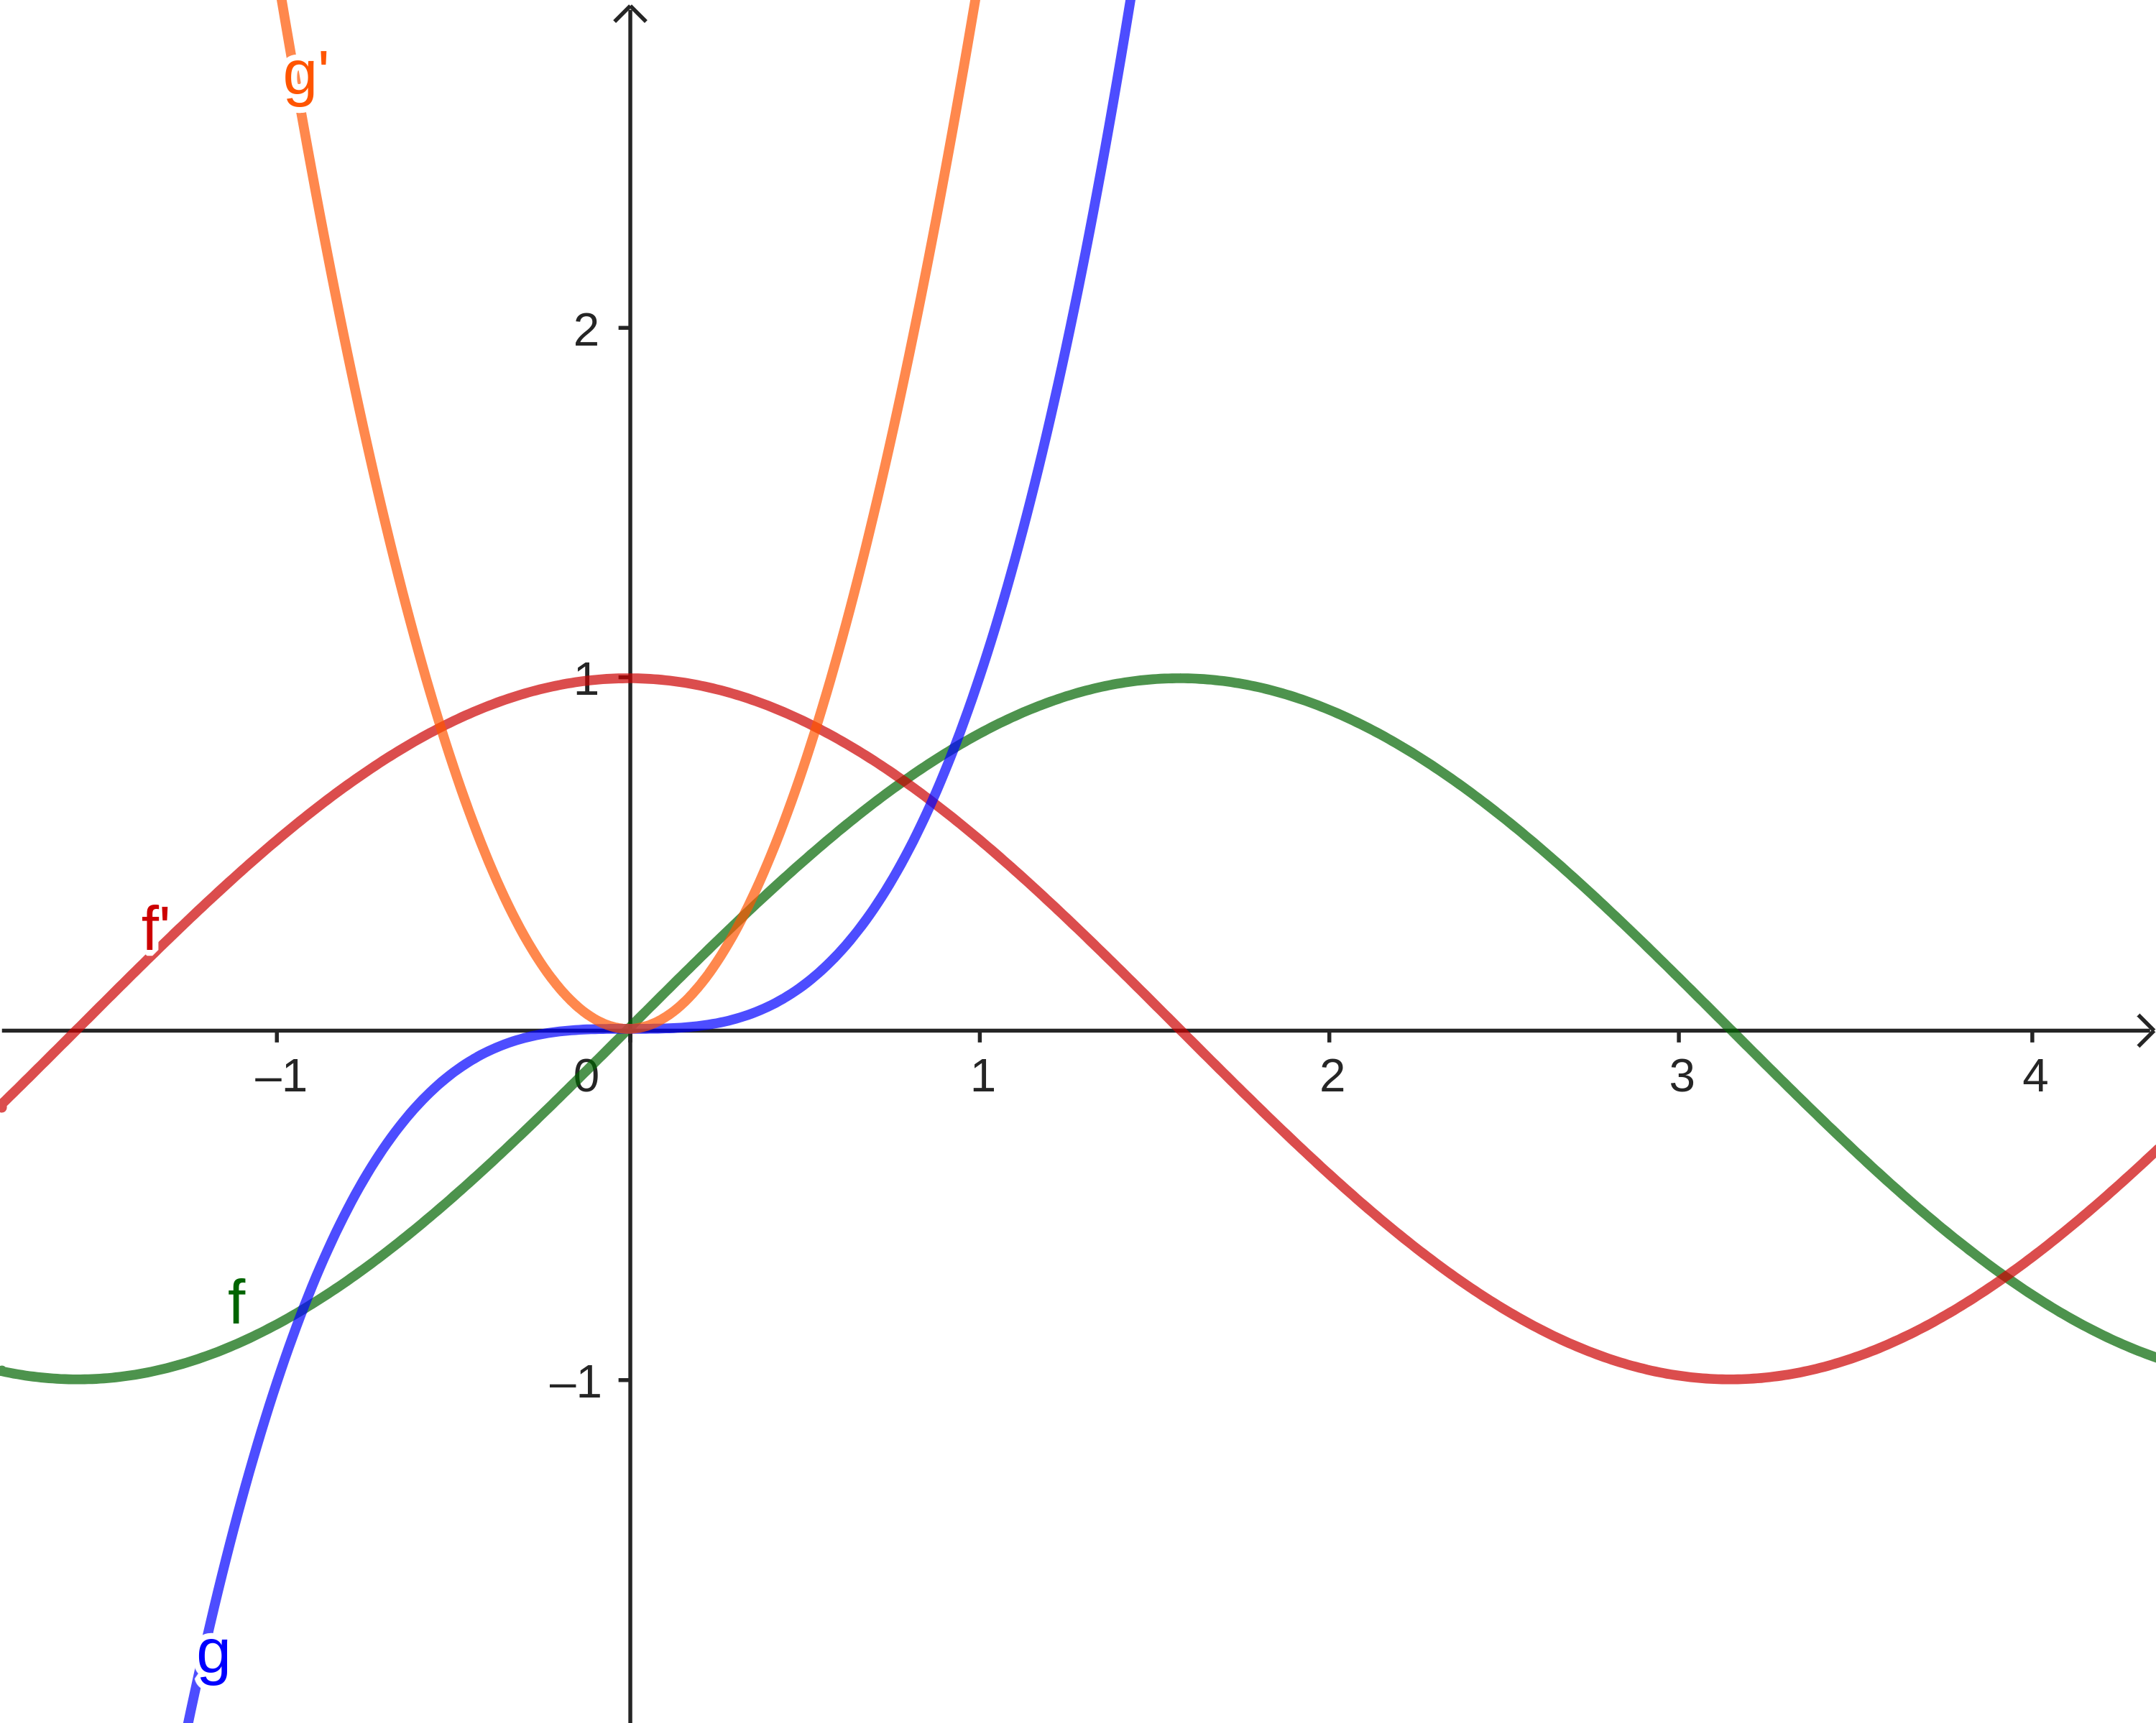
\includegraphics[width=0.65\textwidth]{math-figures/2-abls.png}
  \end{center}
  \caption{Zwei Funktionen und ihre ersten Ableitungen.}
\end{figure}

Hier Sieht man die Funktionen $f(x)=\sin(x)$ und $g(x)=x^3$, sowie ihre
Ableitungen $f'(x)=\cos(x)$ und $g(x)=x^2$.
Die Ableitungsfunktionen zeigen je die steiung die die Tangente an der Stelle
hätte, das ist bei dem $\sin$ -1 bis 1, und bei $x^3$ ist es $-\infty\text{ bis }\infty$.

\subsubsection{Regeln:}
\subsubsection{in general}
\[\frac{d}{dx}[x^n] = nx^{n-1}\]

\subsubsection{product rule}
\[\frac{d}{dx}\left[f(x)*g(x)\right]=f'(x)*g(x)+f(x)*g'(x)\]

\subsubsection{quotient rule}
\[\frac{d}{dx} \left[\frac{f(x)}{g(x)}\right]=
\frac{g(x)*f'(x)-f(x)*g'(x)}{[g(x)]^2}\]

\subsubsection{trig derivatives to remember}
\begin{align*}
    \frac{d}{dx}[\sin x]&=\cos (x)\\
    \frac{d}{dx}[\cos x]&=-\sin(x)\\
    \frac{d}{dx}[\tan x]&=\sec^2 (x)\\
    \frac{d}{dx}[\sec x]&=\sec(x)\tan(x)\\
    \frac{d}{dx}[-\csc x]&=\csc(x)\cot(x)\\
    \frac{d}{dx}[\cot x]&=\csc^2(x)\\
\end{align*}

\begin{align*}
    \frac{d}{dx}\left[\sin^{-1}\right]&= \frac{1}{\sqrt{1-x^2}} \text{where} |x|<1\\
    \frac{d}{dx}\left[\cos^{-1}\right]&= \frac{-1}{\sqrt{1-x^2}} \text{where} |x|<1 \\
    \frac{d}{dx}\left[\tan^{-1}\right]&=\frac{1}{1+x^2}  \\
    \frac{d}{dx}\left[\cot^{-1}\right]&= \frac{-1}{1+x^2} \\
    \frac{d}{dx}\left[\sec^{-1}\right]&=\frac{1}{|x|\sqrt{x_2-1}} \text{where} |x|>1\\
    \frac{d}{dx}\left[\csc^{-1}\right]&= \frac{-1}{|x|\sqrt{x^2-1}} \text{where} |x|>1 \\
    \frac{d}{dx}\left[e^{ax}\right]&= ae^{ax} \\
    \frac{d}{dx}\left[\ln(ax)\right]&= \frac{1}{x} \\
    \frac{d}{dx}\left[\log_bx\right]&= \frac{1}{x \ln b} \\
    \frac{d}{dx}\left[b^x\right]&= b^x \ln b \\
    \frac{d}{dx}\left[\sin h\right]&= \cos h \\
    \frac{d}{dx}\left[\cos h\right]&= \sin h \\
    \frac{d}{dx}\left[\tan h\right]&= \sec h^2= \frac{1}{\cos h^{2}}
\end{align*}

\subsection{Vokabeln}
\begin{figure}[htpb]
  \begin{center}
    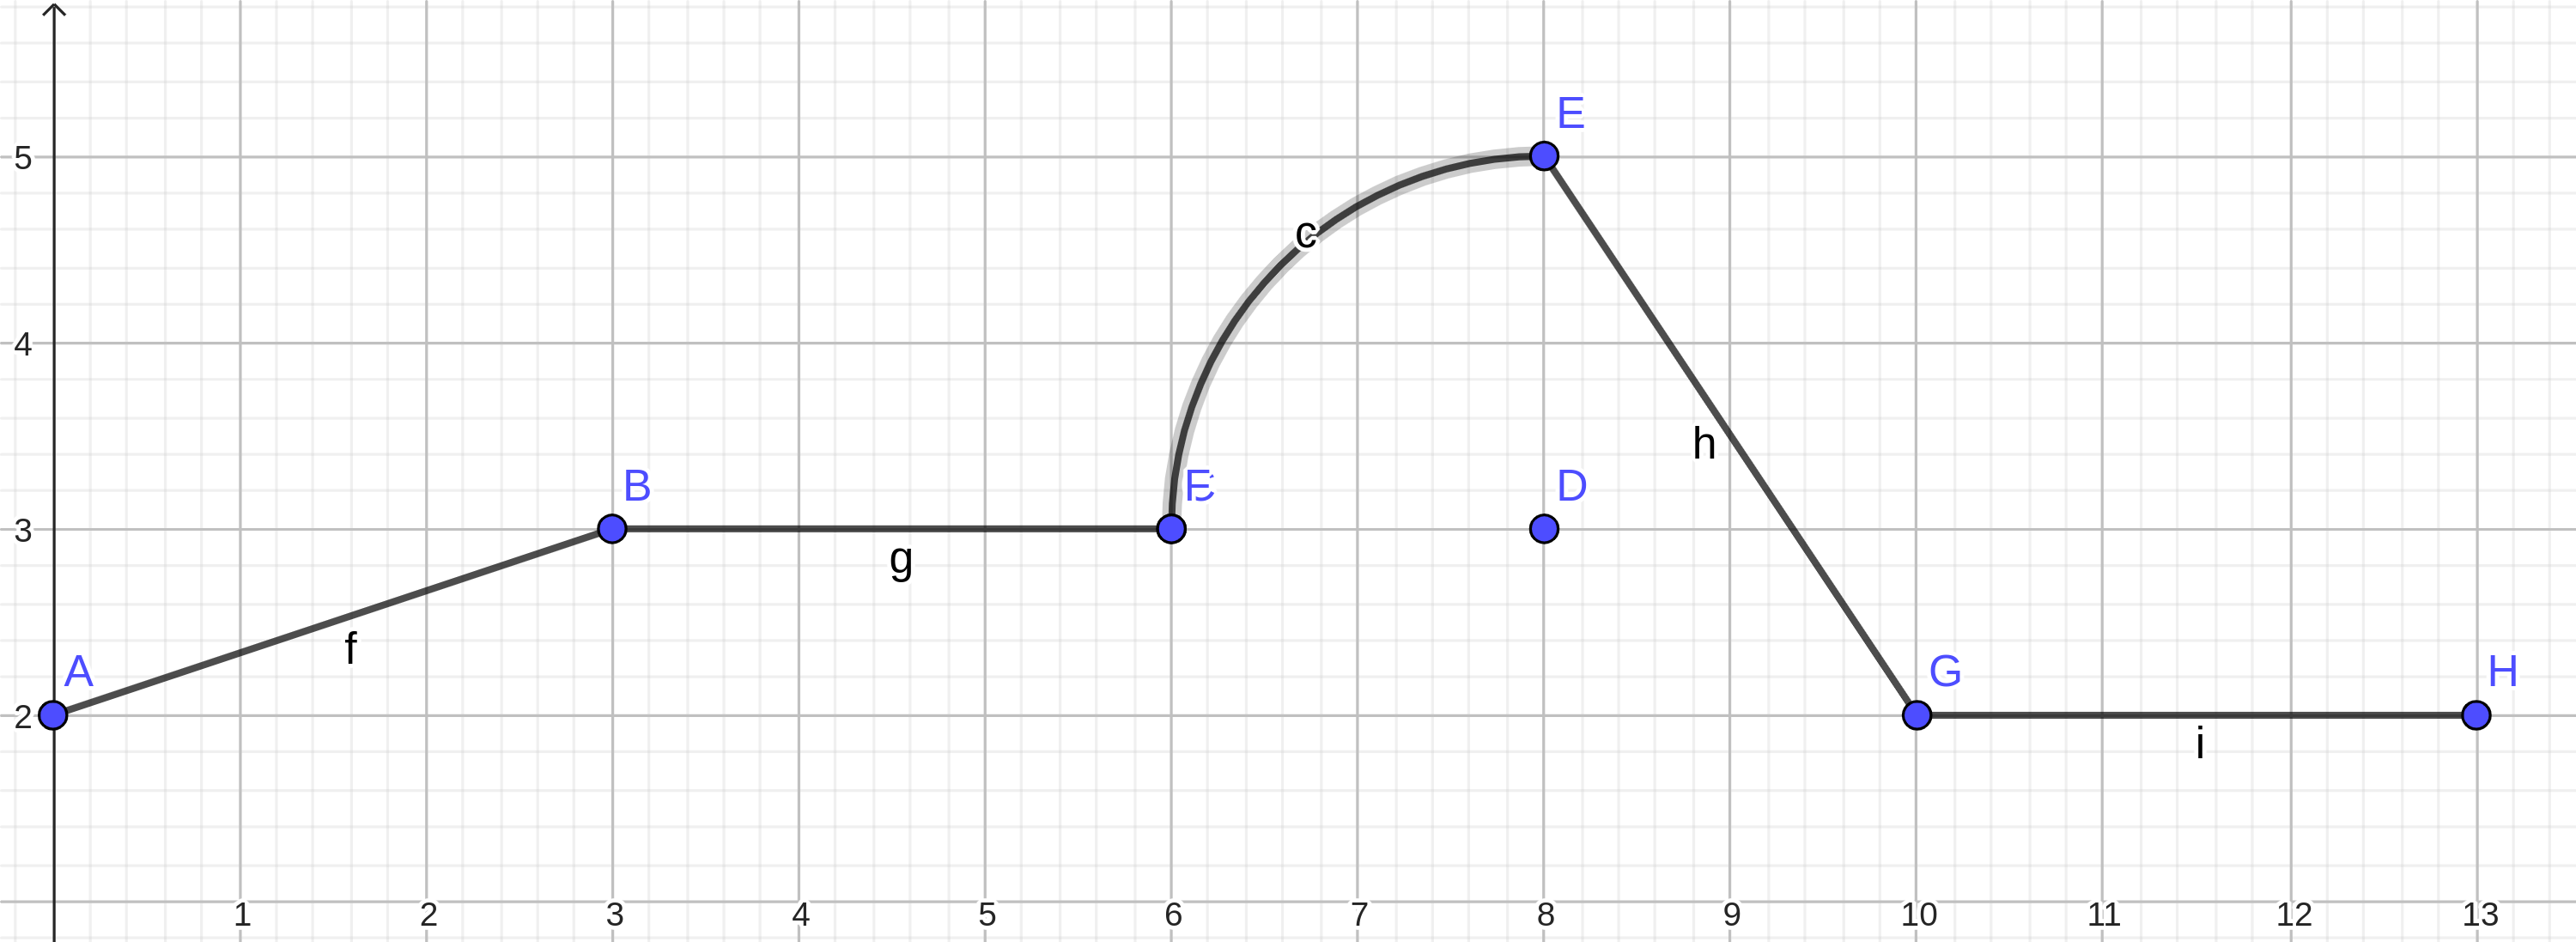
\includegraphics[width=0.75\textwidth]{math-figures/mon.png}
  \end{center}
\end{figure}

f ist \textbf{monomon wachsend} für: [A,B]; [A,F]; [A,E]; [B,F]; [B,E]; [F, E].\\ 
...\textbf{streng monoton wachsend} für: [A,B]; [F,E].\\  
...\textbf{monoton fallend} für: [B,F]; [E,G]; [G,H].\\
...\textbf{streng monoton fallend} für: [E,G].

\begin{itemize}
\item \textbf{Lokales Minimum:} Ein Punkt auf einer Funktion, bei dem der Funktionswert kleiner ist als alle benachbarten Funktionswerte.
\item \textbf{Lokales Maximum:} Ein Punkt auf einer Funktion, bei dem der Funktionswert größer ist als alle benachbarten Funktionswerte.
\item \textbf{Globales Minimum:} Ein Punkt auf einer Funktion, bei dem der Funktionswert kleiner ist als alle anderen Funktionswerte auf der gesamten Funktion.
\item \textbf{Globales Maximum:} Ein Punkt auf einer Funktion, bei dem der Funktionswert größer ist als alle anderen Funktionswerte auf der gesamten Funktion.
\end{itemize}

\subsection{Wie man Extrema findet}
\textbf{Einfach übernommen aus Calculus 1, 3.3 und 3.4}
\section{Calculus 3.3, The First Derivative Test for Increasing and Decreasing} % (fold)
\begin{multicols}{2}
\label{ssub:Calculus 3.3, The First Derivative Test for Increasing and Decreasing}

\begin{tcolorbox}[colback=blue!10!white,colframe=blue!50!black,title=Recall:]
  \[f'(x)> \implies \text{Increasing}\]
  \[f'(x)< \implies \text{Decreasing}\]
  \[f'(x)= \implies \text{Critical Point/Constant}\]
\end{tcolorbox}

\begin{tcolorbox}[colback=red!10!white,colframe=red!50!black,title=How to find relative extrema]
\begin{enumerate}
  \item 1st derivative test
    \subitem take $f'(x)$
  \item set it to =0 for critical numbers
  \item make the f'(x) table
    \begin{center}
      %LaTeX with PSTricks extensions
%%Creator: Inkscape 1.2.2 (b0a8486541, 2022-12-01)
%%Please note this file requires PSTricks extensions
\psset{xunit=.5pt,yunit=.5pt,runit=.5pt}
\begin{pspicture}(302.36220472,113.38582677)
{
\newrgbcolor{curcolor}{0 0 0}
\pscustom[linestyle=none,fillstyle=solid,fillcolor=curcolor]
{
\newpath
\moveto(12.82103939,86.95297269)
\lineto(8.71057011,86.95297269)
\lineto(8.71057011,72.70334586)
\lineto(6.0311531,72.70334586)
\lineto(6.0311531,86.95297269)
\lineto(3.16904857,86.95297269)
\lineto(3.16904857,88.20133744)
\lineto(6.0311531,89.11477506)
\lineto(6.0311531,90.05866059)
\curveto(6.0311531,92.16971642)(6.49802122,93.68196314)(7.43175745,94.59540076)
\curveto(8.36549368,95.52913699)(9.66460496,95.99600511)(11.32909128,95.99600511)
\curveto(11.97864692,95.99600511)(12.56730672,95.93510927)(13.09507068,95.81331758)
\curveto(13.64313325,95.71182452)(14.11000136,95.59003283)(14.49567502,95.44794254)
\lineto(13.79537285,93.34703602)
\curveto(13.47059503,93.44852909)(13.09507068,93.55002215)(12.66879979,93.65151522)
\curveto(12.2425289,93.75300829)(11.80610871,93.80375483)(11.35953921,93.80375483)
\curveto(10.4664002,93.80375483)(9.79654595,93.49927562)(9.34997645,92.89031721)
\curveto(8.92370556,92.30165741)(8.71057011,91.36792118)(8.71057011,90.08910851)
\lineto(8.71057011,89.02343129)
\lineto(12.82103939,89.02343129)
\closepath
}
}
{
\newrgbcolor{curcolor}{0 0 0}
\pscustom[linestyle=none,fillstyle=solid,fillcolor=curcolor]
{
\newpath
\moveto(18.05807755,94.44316116)
\lineto(17.44911914,86.58759765)
\lineto(15.77448351,86.58759765)
\lineto(15.1655251,94.44316116)
\closepath
}
}
{
\newrgbcolor{curcolor}{0 0 0}
\pscustom[linestyle=none,fillstyle=solid,fillcolor=curcolor]
{
\newpath
\moveto(21.25512083,81.0460761)
\curveto(21.25512083,83.52250698)(21.61034657,85.90759409)(22.32079805,88.20133744)
\curveto(23.05154814,90.5153794)(24.18827051,92.59598731)(25.73096515,94.44316116)
\lineto(28.25814256,94.44316116)
\curveto(26.8372396,92.53509147)(25.76141307,90.43418495)(25.03066298,88.1404416)
\curveto(24.3202115,85.84669825)(23.96498576,83.49205906)(23.96498576,81.07652402)
\curveto(23.96498576,78.72188483)(24.3202115,76.40784287)(25.03066298,74.13439813)
\curveto(25.76141307,71.88125201)(26.82709029,69.8006441)(28.22769464,67.89257441)
\lineto(25.73096515,67.89257441)
\curveto(24.18827051,69.67885242)(23.05154814,71.69856448)(22.32079805,73.95171061)
\curveto(21.61034657,76.22515534)(21.25512083,78.58994384)(21.25512083,81.0460761)
\closepath
}
}
{
\newrgbcolor{curcolor}{0 0 0}
\pscustom[linestyle=none,fillstyle=solid,fillcolor=curcolor]
{
\newpath
\moveto(35.62651611,81.0460761)
\lineto(29.9936508,89.02343129)
\lineto(33.03844286,89.02343129)
\lineto(37.2402559,82.87295134)
\lineto(41.41162102,89.02343129)
\lineto(44.42596516,89.02343129)
\lineto(38.79309985,81.0460761)
\lineto(44.73044436,72.70334586)
\lineto(41.68565231,72.70334586)
\lineto(37.2402559,79.21920087)
\lineto(32.73396366,72.70334586)
\lineto(29.71961952,72.70334586)
\closepath
}
}
{
\newrgbcolor{curcolor}{0 0 0}
\pscustom[linestyle=none,fillstyle=solid,fillcolor=curcolor]
{
\newpath
\moveto(53.19494584,81.0460761)
\curveto(53.19494584,78.58994384)(52.8295708,76.22515534)(52.0988207,73.95171061)
\curveto(51.38836922,71.69856448)(50.26179616,69.67885242)(48.71910152,67.89257441)
\lineto(46.22237203,67.89257441)
\curveto(47.62297638,69.8006441)(48.67850429,71.88125201)(49.38895577,74.13439813)
\curveto(50.11970586,76.40784287)(50.48508091,78.72188483)(50.48508091,81.07652402)
\curveto(50.48508091,83.49205906)(50.11970586,85.84669825)(49.38895577,88.1404416)
\curveto(48.67850429,90.43418495)(47.61282707,92.53509147)(46.19192411,94.44316116)
\lineto(48.71910152,94.44316116)
\curveto(50.26179616,92.59598731)(51.38836922,90.5153794)(52.0988207,88.20133744)
\curveto(52.8295708,85.90759409)(53.19494584,83.52250698)(53.19494584,81.0460761)
\closepath
}
}
{
\newrgbcolor{curcolor}{0 0 0}
\pscustom[linestyle=none,fillstyle=solid,fillcolor=curcolor]
{
\newpath
\moveto(63.85170178,78.61024246)
\lineto(75.33056784,83.39056599)
\lineto(63.85170178,88.84074377)
\lineto(63.85170178,91.21568158)
\lineto(78.19267238,84.06042024)
\lineto(78.19267238,82.53802421)
\lineto(63.85170178,76.23530465)
\closepath
}
}
{
\newrgbcolor{curcolor}{0 0 0}
\pscustom[linestyle=none,fillstyle=solid,fillcolor=curcolor]
{
\newpath
\moveto(1.12846303,55.12736523)
\lineto(300.7614447,55.12736523)
\lineto(300.7614447,58.47730209)
\lineto(1.12846303,58.47730209)
\closepath
}
}
{
\newrgbcolor{curcolor}{0 0 0}
\pscustom[linestyle=none,fillstyle=solid,fillcolor=curcolor]
{
\newpath
\moveto(90.83225761,110.35787507)
\lineto(94.18219446,110.35787507)
\lineto(94.18219446,1.90377063)
\lineto(90.83225761,1.90377063)
\closepath
}
}
{
\newrgbcolor{curcolor}{0 0 0}
\pscustom[linestyle=none,fillstyle=solid,fillcolor=curcolor]
{
\newpath
\moveto(162.85584938,83.02399883)
\lineto(164.71692825,83.02399883)
\lineto(164.71692825,57.27139691)
\lineto(162.85584938,57.27139691)
\closepath
}
}
{
\newrgbcolor{curcolor}{0 0 0}
\pscustom[linestyle=none,fillstyle=solid,fillcolor=curcolor]
{
\newpath
\moveto(232.85591666,83.02399883)
\lineto(234.71699553,83.02399883)
\lineto(234.71699553,57.27139691)
\lineto(232.85591666,57.27139691)
\closepath
}
}
{
\newrgbcolor{curcolor}{0 0 0}
\pscustom[linestyle=none,fillstyle=solid,fillcolor=curcolor]
{
\newpath
\moveto(164.30610142,94.7613188)
\lineto(163.82627906,92.22194872)
\lineto(162.07676976,92.22194872)
\lineto(162.07676976,91.42470463)
\lineto(163.68602457,91.42470463)
\lineto(163.30216441,89.50541329)
\lineto(161.63385827,89.50541329)
\lineto(161.63385827,88.7007874)
\lineto(163.14714709,88.7007874)
\lineto(162.68946898,86.19832668)
\lineto(163.53100346,86.19832668)
\lineto(163.99606299,88.7007874)
\lineto(165.70866142,88.7007874)
\lineto(165.22145764,86.19832668)
\lineto(166.07037354,86.19832668)
\lineto(166.56495874,88.7007874)
\lineto(168.36614173,88.7007874)
\lineto(168.36614173,89.50541329)
\lineto(166.71997984,89.50541329)
\lineto(167.08907339,91.42470463)
\lineto(168.77214614,91.42470463)
\lineto(168.77214614,92.22194872)
\lineto(167.25147591,92.22194872)
\lineto(167.73129827,94.7613188)
\lineto(166.8971452,94.7613188)
\lineto(166.41732283,92.22194872)
\lineto(164.68996157,92.22194872)
\lineto(165.16978394,94.7613188)
\closepath
\moveto(164.52017764,91.42470463)
\lineto(166.24015748,91.42470463)
\lineto(165.87106394,89.50541329)
\lineto(164.15108409,89.50541329)
\closepath
}
}
{
\newrgbcolor{curcolor}{0 0 0}
\pscustom[linestyle=none,fillstyle=solid,fillcolor=curcolor]
{
\newpath
\moveto(234.30612283,94.7613188)
\lineto(233.82630047,92.22194872)
\lineto(232.07679118,92.22194872)
\lineto(232.07679118,91.42470463)
\lineto(233.68604598,91.42470463)
\lineto(233.30218583,89.50541329)
\lineto(231.63387969,89.50541329)
\lineto(231.63387969,88.7007874)
\lineto(233.1471685,88.7007874)
\lineto(232.68949039,86.19832668)
\lineto(233.53102488,86.19832668)
\lineto(233.99608441,88.7007874)
\lineto(235.70868283,88.7007874)
\lineto(235.22147906,86.19832668)
\lineto(236.07039496,86.19832668)
\lineto(236.56498016,88.7007874)
\lineto(238.36616315,88.7007874)
\lineto(238.36616315,89.50541329)
\lineto(236.72000126,89.50541329)
\lineto(237.0890948,91.42470463)
\lineto(238.77216756,91.42470463)
\lineto(238.77216756,92.22194872)
\lineto(237.25149732,92.22194872)
\lineto(237.73131969,94.7613188)
\lineto(236.89716661,94.7613188)
\lineto(236.41734425,92.22194872)
\lineto(234.68998299,92.22194872)
\lineto(235.16980535,94.7613188)
\closepath
\moveto(234.52019906,91.42470463)
\lineto(236.2401789,91.42470463)
\lineto(235.87108535,89.50541329)
\lineto(234.15110551,89.50541329)
\closepath
}
}
\end{pspicture}

    \end{center}
  \item Find the sign of \textit{each interval}, by
    plugging into $f'(x)$ (this tells you
    increasing/decreasing)
\end{enumerate}
\end{tcolorbox}

\textbf{example}\\
\begin{align*}
  f(x)&=x^3-3x+1\\
  f'(x)&=3x^2-3\\
  3^2-3&=0\\
  \implies x^2-1&=0\\
  \implies x&=\pm 1
\end{align*}

\begin{center}
%LaTeX with PSTricks extensions
%%Creator: Inkscape 1.2.2 (b0a8486541, 2022-12-01)
%%Please note this file requires PSTricks extensions
\psset{xunit=.5pt,yunit=.5pt,runit=.5pt}
\begin{pspicture}(302.36220472,113.38582677)
{
\newrgbcolor{curcolor}{0 0 0}
\pscustom[linestyle=none,fillstyle=solid,fillcolor=curcolor]
{
\newpath
\moveto(12.82103939,86.95297269)
\lineto(8.71057011,86.95297269)
\lineto(8.71057011,72.70334586)
\lineto(6.0311531,72.70334586)
\lineto(6.0311531,86.95297269)
\lineto(3.16904857,86.95297269)
\lineto(3.16904857,88.20133744)
\lineto(6.0311531,89.11477506)
\lineto(6.0311531,90.05866059)
\curveto(6.0311531,92.16971642)(6.49802122,93.68196314)(7.43175745,94.59540076)
\curveto(8.36549368,95.52913699)(9.66460496,95.99600511)(11.32909128,95.99600511)
\curveto(11.97864692,95.99600511)(12.56730672,95.93510927)(13.09507068,95.81331758)
\curveto(13.64313325,95.71182452)(14.11000136,95.59003283)(14.49567502,95.44794254)
\lineto(13.79537285,93.34703602)
\curveto(13.47059503,93.44852909)(13.09507068,93.55002215)(12.66879979,93.65151522)
\curveto(12.2425289,93.75300829)(11.80610871,93.80375483)(11.35953921,93.80375483)
\curveto(10.4664002,93.80375483)(9.79654595,93.49927562)(9.34997645,92.89031721)
\curveto(8.92370556,92.30165741)(8.71057011,91.36792118)(8.71057011,90.08910851)
\lineto(8.71057011,89.02343129)
\lineto(12.82103939,89.02343129)
\closepath
}
}
{
\newrgbcolor{curcolor}{0 0 0}
\pscustom[linestyle=none,fillstyle=solid,fillcolor=curcolor]
{
\newpath
\moveto(18.05807755,94.44316116)
\lineto(17.44911914,86.58759765)
\lineto(15.77448351,86.58759765)
\lineto(15.1655251,94.44316116)
\closepath
}
}
{
\newrgbcolor{curcolor}{0 0 0}
\pscustom[linestyle=none,fillstyle=solid,fillcolor=curcolor]
{
\newpath
\moveto(21.25512083,81.0460761)
\curveto(21.25512083,83.52250698)(21.61034657,85.90759409)(22.32079805,88.20133744)
\curveto(23.05154814,90.5153794)(24.18827051,92.59598731)(25.73096515,94.44316116)
\lineto(28.25814256,94.44316116)
\curveto(26.8372396,92.53509147)(25.76141307,90.43418495)(25.03066298,88.1404416)
\curveto(24.3202115,85.84669825)(23.96498576,83.49205906)(23.96498576,81.07652402)
\curveto(23.96498576,78.72188483)(24.3202115,76.40784287)(25.03066298,74.13439813)
\curveto(25.76141307,71.88125201)(26.82709029,69.8006441)(28.22769464,67.89257441)
\lineto(25.73096515,67.89257441)
\curveto(24.18827051,69.67885242)(23.05154814,71.69856448)(22.32079805,73.95171061)
\curveto(21.61034657,76.22515534)(21.25512083,78.58994384)(21.25512083,81.0460761)
\closepath
}
}
{
\newrgbcolor{curcolor}{0 0 0}
\pscustom[linestyle=none,fillstyle=solid,fillcolor=curcolor]
{
\newpath
\moveto(35.62651611,81.0460761)
\lineto(29.9936508,89.02343129)
\lineto(33.03844286,89.02343129)
\lineto(37.2402559,82.87295134)
\lineto(41.41162102,89.02343129)
\lineto(44.42596516,89.02343129)
\lineto(38.79309985,81.0460761)
\lineto(44.73044436,72.70334586)
\lineto(41.68565231,72.70334586)
\lineto(37.2402559,79.21920087)
\lineto(32.73396366,72.70334586)
\lineto(29.71961952,72.70334586)
\closepath
}
}
{
\newrgbcolor{curcolor}{0 0 0}
\pscustom[linestyle=none,fillstyle=solid,fillcolor=curcolor]
{
\newpath
\moveto(53.19494584,81.0460761)
\curveto(53.19494584,78.58994384)(52.8295708,76.22515534)(52.0988207,73.95171061)
\curveto(51.38836922,71.69856448)(50.26179616,69.67885242)(48.71910152,67.89257441)
\lineto(46.22237203,67.89257441)
\curveto(47.62297638,69.8006441)(48.67850429,71.88125201)(49.38895577,74.13439813)
\curveto(50.11970586,76.40784287)(50.48508091,78.72188483)(50.48508091,81.07652402)
\curveto(50.48508091,83.49205906)(50.11970586,85.84669825)(49.38895577,88.1404416)
\curveto(48.67850429,90.43418495)(47.61282707,92.53509147)(46.19192411,94.44316116)
\lineto(48.71910152,94.44316116)
\curveto(50.26179616,92.59598731)(51.38836922,90.5153794)(52.0988207,88.20133744)
\curveto(52.8295708,85.90759409)(53.19494584,83.52250698)(53.19494584,81.0460761)
\closepath
}
}
{
\newrgbcolor{curcolor}{0 0 0}
\pscustom[linestyle=none,fillstyle=solid,fillcolor=curcolor]
{
\newpath
\moveto(63.85170178,78.61024246)
\lineto(75.33056784,83.39056599)
\lineto(63.85170178,88.84074377)
\lineto(63.85170178,91.21568158)
\lineto(78.19267238,84.06042024)
\lineto(78.19267238,82.53802421)
\lineto(63.85170178,76.23530465)
\closepath
}
}
{
\newrgbcolor{curcolor}{0 0 0}
\pscustom[linestyle=none,fillstyle=solid,fillcolor=curcolor]
{
\newpath
\moveto(1.12846303,55.12736523)
\lineto(300.7614447,55.12736523)
\lineto(300.7614447,58.47730209)
\lineto(1.12846303,58.47730209)
\closepath
}
}
{
\newrgbcolor{curcolor}{0 0 0}
\pscustom[linestyle=none,fillstyle=solid,fillcolor=curcolor]
{
\newpath
\moveto(90.83225761,110.35787507)
\lineto(94.18219446,110.35787507)
\lineto(94.18219446,1.90377063)
\lineto(90.83225761,1.90377063)
\closepath
}
}
{
\newrgbcolor{curcolor}{0 0 0}
\pscustom[linestyle=none,fillstyle=solid,fillcolor=curcolor]
{
\newpath
\moveto(162.85584938,83.02399883)
\lineto(164.71692825,83.02399883)
\lineto(164.71692825,57.27139691)
\lineto(162.85584938,57.27139691)
\closepath
}
}
{
\newrgbcolor{curcolor}{0 0 0}
\pscustom[linestyle=none,fillstyle=solid,fillcolor=curcolor]
{
\newpath
\moveto(232.85591666,83.02399883)
\lineto(234.71699553,83.02399883)
\lineto(234.71699553,57.27139691)
\lineto(232.85591666,57.27139691)
\closepath
}
}
{
\newrgbcolor{curcolor}{0 0 0}
\pscustom[linestyle=none,fillstyle=solid,fillcolor=curcolor]
{
\newpath
\moveto(129.48084283,97.90142513)
\lineto(129.48084283,79.33734009)
\lineto(129.48084283,74.03314016)
\curveto(129.48287318,72.71172318)(131.46398666,72.71172318)(131.46601701,74.03314016)
\lineto(131.46601701,79.33734009)
\lineto(131.46601701,97.90142513)
\curveto(131.46398666,99.22284211)(129.48287318,99.22284211)(129.48084283,97.90142513)
\closepath
}
}
{
\newrgbcolor{curcolor}{0 0 0}
\pscustom[linestyle=none,fillstyle=solid,fillcolor=curcolor]
{
\newpath
\moveto(113.54644157,84.67658835)
\curveto(115.52759055,84.31688693)(119.3345726,83.66914091)(124.54116283,83.1409886)
\curveto(129.65228976,82.62252094)(136.20356031,82.19665398)(145.3900611,82.14963704)
\curveto(145.78738772,82.14835389)(146.10684472,82.14818117)(146.29256315,82.14818117)
\curveto(147.61564826,82.14854629)(147.61564826,84.13372273)(146.29256315,84.13335761)
\curveto(146.10816,84.13335761)(145.79095937,84.1335292)(145.39834583,84.13479534)
\curveto(136.27390866,84.18149631)(129.78620598,84.60430035)(124.74151181,85.11602986)
\curveto(119.60183433,85.63739414)(115.84876724,86.27620535)(113.90107465,86.62983156)
\curveto(112.59969876,86.86512055)(112.24506569,84.91187734)(113.54644157,84.67658835)
\closepath
}
}
{
\newrgbcolor{curcolor}{0 0 0}
\pscustom[linestyle=none,fillstyle=solid,fillcolor=curcolor]
{
\newpath
\moveto(193.92576378,85.81220863)
\curveto(194.43150992,85.80695509)(195.27098835,85.88507792)(196.17380409,85.92804359)
\curveto(196.49423244,85.94331288)(196.82301732,85.94826406)(197.14340787,85.9239995)
\curveto(197.40506457,85.90415698)(197.66140346,85.86508422)(197.91250772,85.79526123)
\curveto(197.96296441,85.76540296)(198.01878803,85.72739225)(198.08273764,85.67846249)
\curveto(198.1054148,85.66122784)(198.12899906,85.64248139)(198.15435969,85.6218565)
\curveto(198.26373921,85.5329091)(198.39889512,85.40946973)(198.57702803,85.25475855)
\curveto(198.72257764,85.12834847)(198.92636976,84.95695824)(199.16496756,84.80689247)
\curveto(199.37590299,84.67423483)(199.63644094,84.54320617)(199.95031559,84.46143231)
\curveto(201.36549921,83.9641251)(202.85766425,83.68519672)(204.44682709,83.54716082)
\curveto(205.93751433,83.41767798)(207.43159181,83.41803704)(208.94688378,83.44196523)
\curveto(212.28780094,83.5220383)(215.66003906,83.84164989)(218.88752126,83.84302791)
\curveto(219.41149228,83.83913499)(219.7715452,83.85595389)(220.16070425,83.81154444)
\curveto(220.34476724,83.79056806)(220.49693102,83.75823798)(220.62601323,83.71463357)
\curveto(220.75909039,83.66967609)(220.86692031,83.61291137)(220.95880063,83.54404838)
\lineto(220.8998778,83.59185184)
\curveto(220.90112126,83.59076107)(220.90112126,83.58950665)(220.89877417,83.59759672)
\curveto(221.26784408,82.32841135)(223.17151746,82.87934471)(222.80569701,84.14947049)
\curveto(222.7369474,84.38701002)(222.57673323,84.761808)(222.20851654,85.08461329)
\curveto(222.1896189,85.10128101)(222.16981417,85.11723061)(222.1495937,85.13241676)
\curveto(221.8720252,85.34048731)(221.5724863,85.4902662)(221.26148787,85.59534274)
\curveto(220.9676674,85.69461203)(220.67191937,85.75127849)(220.38564661,85.78392227)
\curveto(219.85725732,85.8441755)(219.3062778,85.82510022)(218.89446803,85.82814274)
\curveto(215.53356472,85.82673789)(212.1454148,85.5043355)(208.90745197,85.42669871)
\curveto(207.41240693,85.40311446)(206.00280945,85.40462627)(204.61864441,85.52485682)
\curveto(203.1355389,85.65368202)(201.80114646,85.91061506)(200.56871055,86.34835616)
\curveto(200.53431685,86.36052624)(200.49962079,86.37076876)(200.4642822,86.37912151)
\curveto(200.38959874,86.39673411)(200.31245858,86.43036435)(200.22186331,86.48733694)
\curveto(200.1179263,86.55271143)(200.00832,86.64106545)(199.8787578,86.75356309)
\curveto(199.72678299,86.88553285)(199.58051528,87.02082104)(199.40690646,87.16199773)
\curveto(199.3681285,87.19351899)(199.32904819,87.22446954)(199.28943874,87.25479647)
\curveto(199.12846866,87.37800529)(198.9457663,87.50102135)(198.73684535,87.60565757)
\curveto(198.68801386,87.63011112)(198.63721701,87.65051301)(198.58502173,87.66661757)
\curveto(198.13278236,87.80615773)(197.69473134,87.87306671)(197.29348535,87.90347301)
\curveto(196.85736567,87.93650608)(196.43752063,87.92800214)(196.07949732,87.91095647)
\curveto(195.05170016,87.86204183)(194.34374929,87.7931297)(193.94644913,87.79725694)
\curveto(192.62307033,87.81111519)(192.60228293,85.82604608)(193.92566173,85.81218784)
\closepath
}
}
{
\newrgbcolor{curcolor}{0 0 0}
\pscustom[linestyle=none,fillstyle=solid,fillcolor=curcolor]
{
\newpath
\moveto(278.39286425,101.37257726)
\curveto(278.1684737,100.41267213)(278.0740611,99.28338331)(278.22452409,97.67871458)
\curveto(278.32505953,96.60636321)(278.53111937,95.44097272)(278.66448378,94.28477745)
\curveto(278.76418772,93.42927307)(278.86415622,92.55187654)(278.84624126,91.71196044)
\curveto(278.83754835,91.30426129)(278.80122709,90.91368416)(278.7274885,90.54117846)
\curveto(278.6571137,90.18581972)(278.55340346,89.85065839)(278.40951685,89.53430211)
\curveto(278.36253732,89.46255156)(278.30327433,89.38908132)(278.22889323,89.3105125)
\curveto(278.1971452,89.27683691)(278.16207118,89.24192164)(278.12340661,89.20513172)
\curveto(277.97347276,89.06248857)(277.82856567,88.94651754)(277.5990274,88.75405266)
\curveto(277.41212976,88.59735723)(277.16985071,88.38980069)(276.94955717,88.143264)
\curveto(276.7412674,87.91014652)(276.53148472,87.62012258)(276.37831559,87.25614954)
\curveto(275.82207874,86.10264227)(275.49465071,84.88767572)(275.26686614,83.64340989)
\curveto(275.04738898,82.44458079)(274.91990551,81.20861934)(274.76895496,80.07142828)
\curveto(274.5462274,78.03547654)(274.25120126,76.33300271)(273.60866268,74.77104794)
\curveto(273.2652926,73.85617172)(272.90649071,73.0171166)(272.60179276,72.24669014)
\curveto(272.15424756,71.11506557)(271.89041008,70.31681802)(271.69824756,69.56944668)
\curveto(271.37117558,68.28916277)(273.28984874,67.79583514)(273.62088567,69.07509959)
\curveto(273.78673134,69.72015156)(274.02091087,70.43710148)(274.44784252,71.5165988)
\curveto(274.7408315,72.25739376)(275.1015874,73.09918526)(275.45607685,74.04510652)
\curveto(276.19572661,75.84181644)(276.5140989,77.76878513)(276.73963087,79.83300737)
\curveto(276.89837102,81.02689663)(277.01175685,82.15058721)(277.21959307,83.28593083)
\curveto(277.43041512,84.43756611)(277.7187137,85.47221102)(278.17712504,86.4159428)
\curveto(278.18657386,86.43563414)(278.19564472,86.45560517)(278.20395969,86.47587099)
\curveto(278.25059906,86.59060233)(278.32297701,86.70077934)(278.43001323,86.82053367)
\curveto(278.54744315,86.9519365)(278.69382425,87.08123036)(278.87462551,87.2328189)
\curveto(279.06549165,87.39285165)(279.28306394,87.56820661)(279.49187906,87.76686841)
\curveto(279.5523137,87.82435502)(279.61206803,87.88384479)(279.6707263,87.94580258)
\curveto(279.83060031,88.11468321)(279.99357354,88.31397014)(280.13557795,88.55064454)
\curveto(280.15258583,88.57902879)(280.16808189,88.60827477)(280.18233071,88.63823131)
\curveto(280.41552756,89.13309128)(280.57330016,89.64206929)(280.67498079,90.15556157)
\curveto(280.77574299,90.66442583)(280.8204926,91.17299414)(280.83111307,91.66955301)
\curveto(280.85227843,92.66846967)(280.73363906,93.68108712)(280.63661858,94.51343395)
\curveto(280.49280756,95.76013569)(280.29219024,96.89363868)(280.20120567,97.86404183)
\curveto(280.06748598,99.29025524)(280.15793008,100.20116258)(280.32611906,100.92072454)
\curveto(280.62735407,102.20956051)(278.69409927,102.66141324)(278.39286425,101.37257726)
\closepath
}
}
{
\newrgbcolor{curcolor}{0 0 0}
\pscustom[linestyle=none,fillstyle=solid,fillcolor=curcolor]
{
\newpath
\moveto(266.14372535,84.21047169)
\curveto(266.60957102,84.02082633)(267.20775307,83.85817814)(268.08515906,83.79686702)
\curveto(268.68754394,83.75477443)(269.21907024,83.7682938)(269.82461858,83.76001663)
\curveto(270.88884283,83.77891427)(271.92248315,83.82907994)(272.96628661,83.89711521)
\curveto(274.16596913,83.97531364)(275.27046425,84.06852813)(276.71423622,84.18871332)
\curveto(278.66881134,84.35142198)(281.08380094,84.55301443)(283.41174425,84.56629946)
\curveto(283.89094299,84.54898923)(284.33920252,84.55050104)(284.76669354,84.5073086)
\curveto(284.96999433,84.48674797)(285.15764409,84.45695017)(285.33152504,84.41331175)
\curveto(285.48512504,84.37476813)(285.6254589,84.32605002)(285.7546885,84.26491238)
\curveto(286.64357291,83.69151912)(287.60002016,83.28990085)(288.56749984,83.02407345)
\curveto(289.60408063,82.73925959)(290.64315969,82.61325619)(291.61430929,82.59092939)
\curveto(292.16250709,82.56791206)(292.70219339,82.56696718)(292.94514142,82.56692939)
\curveto(294.26825934,82.56711062)(294.26848611,84.55228706)(292.94536819,84.55210583)
\curveto(292.70612409,84.55213342)(292.20127748,84.55319887)(291.67844787,84.57497197)
\curveto(290.82454299,84.59477669)(289.95083339,84.70272)(289.0934589,84.93829795)
\curveto(288.27941291,85.16196661)(287.49850583,85.4956989)(286.78912252,85.96019565)
\curveto(286.75813039,85.98056731)(286.72577764,85.99916258)(286.69259339,86.01591345)
\curveto(286.40013354,86.16351912)(286.10406047,86.26615597)(285.8147452,86.33876447)
\curveto(285.52319244,86.41193613)(285.23631118,86.45512479)(284.96630173,86.48241298)
\curveto(284.4501052,86.53458557)(283.83674835,86.53700069)(283.46414362,86.55087534)
\curveto(283.45015937,86.55139805)(283.43617512,86.55162293)(283.42200189,86.55154923)
\curveto(280.99735937,86.53888781)(278.49650646,86.32911269)(276.54951685,86.1670337)
\curveto(275.1011263,86.04646299)(274.0155326,85.95488504)(272.8371326,85.8780737)
\curveto(271.81438866,85.81140661)(270.81308598,85.76302488)(269.82004913,85.74492094)
\curveto(269.15788346,85.75448315)(268.75213606,85.74027213)(268.22350866,85.77719811)
\curveto(267.54439937,85.82465008)(267.15317669,85.94286992)(266.89220787,86.04910866)
\curveto(265.66709463,86.54656292)(264.91858187,84.70790818)(266.14369512,84.21045392)
\closepath
}
}
{
\newrgbcolor{curcolor}{1 0 0}
\pscustom[linestyle=none,fillstyle=solid,fillcolor=curcolor]
{
\newpath
\moveto(101.31818857,36.00835745)
\lineto(99.69818859,36.00835745)
\lineto(99.69818859,30.39235753)
\lineto(98.64218861,30.39235753)
\lineto(98.64218861,36.00835745)
\lineto(97.51418862,36.00835745)
\lineto(97.51418862,36.50035744)
\lineto(98.64218861,36.86035744)
\lineto(98.64218861,37.23235743)
\curveto(98.64218861,38.06435742)(98.8261886,38.66035741)(99.1941886,39.0203574)
\curveto(99.56218859,39.3883574)(100.07418859,39.5723574)(100.73018858,39.5723574)
\curveto(100.98618857,39.5723574)(101.21818857,39.5483574)(101.42618857,39.5003574)
\curveto(101.64218856,39.4603574)(101.82618856,39.4123574)(101.97818856,39.3563574)
\lineto(101.70218856,38.52835741)
\curveto(101.57418856,38.56835741)(101.42618857,38.60835741)(101.25818857,38.64835741)
\curveto(101.09018857,38.68835741)(100.91818857,38.70835741)(100.74218858,38.70835741)
\curveto(100.39018858,38.70835741)(100.12618858,38.58835741)(99.95018859,38.34835741)
\curveto(99.78218859,38.11635742)(99.69818859,37.74835742)(99.69818859,37.24435743)
\lineto(99.69818859,36.82435744)
\lineto(101.31818857,36.82435744)
\closepath
}
}
{
\newrgbcolor{curcolor}{1 0 0}
\pscustom[linestyle=none,fillstyle=solid,fillcolor=curcolor]
{
\newpath
\moveto(103.38218695,38.9603574)
\lineto(103.14218695,35.86435745)
\lineto(102.48218696,35.86435745)
\lineto(102.24218697,38.9603574)
\closepath
}
}
{
\newrgbcolor{curcolor}{1 0 0}
\pscustom[linestyle=none,fillstyle=solid,fillcolor=curcolor]
{
\newpath
\moveto(104.64219155,33.68035748)
\curveto(104.64219155,34.65635747)(104.78219155,35.59635746)(105.06219154,36.50035744)
\curveto(105.35019154,37.41235743)(105.79819153,38.23235742)(106.40619152,38.9603574)
\lineto(107.40219151,38.9603574)
\curveto(106.84219152,38.20835742)(106.41819152,37.38035743)(106.13019153,36.47635744)
\curveto(105.85019153,35.57235746)(105.71019153,34.64435747)(105.71019153,33.69235748)
\curveto(105.71019153,32.7643575)(105.85019153,31.85235751)(106.13019153,30.95635752)
\curveto(106.41819152,30.06835754)(106.83819152,29.24835755)(107.39019151,28.49635756)
\lineto(106.40619152,28.49635756)
\curveto(105.79819153,29.20035755)(105.35019154,29.99635754)(105.06219154,30.88435753)
\curveto(104.78219155,31.78035751)(104.64219155,32.7123575)(104.64219155,33.68035748)
\closepath
}
}
{
\newrgbcolor{curcolor}{1 0 0}
\pscustom[linestyle=none,fillstyle=solid,fillcolor=curcolor]
{
\newpath
\moveto(108.24218203,33.14035749)
\lineto(108.24218203,34.07635748)
\lineto(111.14618199,34.07635748)
\lineto(111.14618199,33.14035749)
\closepath
}
}
{
\newrgbcolor{curcolor}{1 0 0}
\pscustom[linestyle=none,fillstyle=solid,fillcolor=curcolor]
{
\newpath
\moveto(117.86618853,30.39235753)
\lineto(112.20218861,30.39235753)
\lineto(112.20218861,31.26835752)
\lineto(114.44618858,33.53635749)
\curveto(114.87818857,33.96835748)(115.24218857,34.35235747)(115.53818856,34.68835747)
\curveto(115.83418856,35.02435746)(116.05818856,35.35235746)(116.21018855,35.67235745)
\curveto(116.36218855,36.00035745)(116.43818855,36.35635744)(116.43818855,36.74035744)
\curveto(116.43818855,37.21235743)(116.29818855,37.56835743)(116.01818856,37.80835742)
\curveto(115.73818856,38.05635742)(115.37418857,38.18035742)(114.92618857,38.18035742)
\curveto(114.51018858,38.18035742)(114.14218859,38.10835742)(113.82218859,37.96435742)
\curveto(113.5101886,37.82035742)(113.1901886,37.62035742)(112.86218861,37.36435743)
\lineto(112.29818861,38.07235742)
\curveto(112.63418861,38.35235741)(113.0181886,38.58835741)(113.4501886,38.78035741)
\curveto(113.89018859,38.9803574)(114.38218858,39.0803574)(114.92618857,39.0803574)
\curveto(115.72618856,39.0803574)(116.35818855,38.87635741)(116.82218855,38.46835741)
\curveto(117.28618854,38.06835742)(117.51818854,37.51235743)(117.51818854,36.80035744)
\curveto(117.51818854,36.35235744)(117.42618854,35.93235745)(117.24218854,35.54035746)
\curveto(117.05818854,35.14835746)(116.80218855,34.76035747)(116.47418855,34.37635747)
\curveto(116.14618856,34.00035748)(115.76218856,33.59635749)(115.32218857,33.16435749)
\lineto(113.53418859,31.40035752)
\lineto(113.53418859,31.35235752)
\lineto(117.86618853,31.35235752)
\closepath
}
}
{
\newrgbcolor{curcolor}{1 0 0}
\pscustom[linestyle=none,fillstyle=solid,fillcolor=curcolor]
{
\newpath
\moveto(121.61019444,33.68035748)
\curveto(121.61019444,32.7123575)(121.46619444,31.78035751)(121.17819445,30.88435753)
\curveto(120.89819445,29.99635754)(120.45419446,29.20035755)(119.84619447,28.49635756)
\lineto(118.86219448,28.49635756)
\curveto(119.41419447,29.24835755)(119.83019447,30.06835754)(120.11019446,30.95635752)
\curveto(120.39819446,31.85235751)(120.54219446,32.7643575)(120.54219446,33.69235748)
\curveto(120.54219446,34.64435747)(120.39819446,35.57235746)(120.11019446,36.47635744)
\curveto(119.83019447,37.38035743)(119.41019447,38.20835742)(118.85019448,38.9603574)
\lineto(119.84619447,38.9603574)
\curveto(120.45419446,38.23235742)(120.89819445,37.41235743)(121.17819445,36.50035744)
\curveto(121.46619444,35.59635746)(121.61019444,34.65635747)(121.61019444,33.68035748)
\closepath
}
}
{
\newrgbcolor{curcolor}{1 0 0}
\pscustom[linestyle=none,fillstyle=solid,fillcolor=curcolor]
{
\newpath
\moveto(122.69018496,32.7203575)
\lineto(127.21418489,34.60435747)
\lineto(122.69018496,36.75235744)
\lineto(122.69018496,37.68835742)
\lineto(128.34218488,34.86835747)
\lineto(128.34218488,34.26835748)
\lineto(122.69018496,31.78435751)
\closepath
}
}
{
\newrgbcolor{curcolor}{1 0 0}
\pscustom[linestyle=none,fillstyle=solid,fillcolor=curcolor]
{
\newpath
\moveto(135.23018894,34.68835747)
\curveto(135.23018894,33.76835748)(135.13418894,32.97635749)(134.94218894,32.3123575)
\curveto(134.75018894,31.65635751)(134.44618895,31.15235752)(134.03018895,30.80035753)
\curveto(133.61418896,30.44835753)(133.06218897,30.27235754)(132.37418898,30.27235754)
\curveto(131.40618899,30.27235754)(130.690189,30.66035753)(130.22618901,31.43635752)
\curveto(129.77018902,32.22035751)(129.54218902,33.30435749)(129.54218902,34.68835747)
\curveto(129.54218902,35.61635745)(129.63418902,36.40835744)(129.81818902,37.06435743)
\curveto(130.01018901,37.72035742)(130.31418901,38.22035742)(130.730189,38.56435741)
\curveto(131.146189,38.91635741)(131.69418899,39.0923574)(132.37418898,39.0923574)
\curveto(133.33418896,39.0923574)(134.05018895,38.70435741)(134.52218895,37.92835742)
\curveto(134.99418894,37.16035743)(135.23018894,36.08035745)(135.23018894,34.68835747)
\closepath
\moveto(130.59818901,34.68835747)
\curveto(130.59818901,33.51235749)(130.730189,32.6323575)(130.994189,32.04835751)
\curveto(131.266189,31.46435752)(131.72618899,31.17235752)(132.37418898,31.17235752)
\curveto(133.01418897,31.17235752)(133.47018896,31.46035752)(133.74218896,32.03635751)
\curveto(134.02218895,32.6203575)(134.16218895,33.50435749)(134.16218895,34.68835747)
\curveto(134.16218895,35.85635745)(134.02218895,36.73235744)(133.74218896,37.31635743)
\curveto(133.47018896,37.90035742)(133.01418897,38.19235742)(132.37418898,38.19235742)
\curveto(131.72618899,38.19235742)(131.266189,37.90035742)(130.994189,37.31635743)
\curveto(130.730189,36.73235744)(130.59818901,35.85635745)(130.59818901,34.68835747)
\closepath
}
}
{
\newrgbcolor{curcolor}{1 0 0}
\pscustom[linestyle=none,fillstyle=solid,fillcolor=curcolor]
{
\newpath
\moveto(179.31825633,36.00835745)
\lineto(177.69825635,36.00835745)
\lineto(177.69825635,30.39235753)
\lineto(176.64225637,30.39235753)
\lineto(176.64225637,36.00835745)
\lineto(175.51425639,36.00835745)
\lineto(175.51425639,36.50035744)
\lineto(176.64225637,36.86035744)
\lineto(176.64225637,37.23235743)
\curveto(176.64225637,38.06435742)(176.82625637,38.66035741)(177.19425636,39.0203574)
\curveto(177.56225636,39.3883574)(178.07425635,39.5723574)(178.73025634,39.5723574)
\curveto(178.98625634,39.5723574)(179.21825633,39.5483574)(179.42625633,39.5003574)
\curveto(179.64225633,39.4603574)(179.82625632,39.4123574)(179.97825632,39.3563574)
\lineto(179.70225632,38.52835741)
\curveto(179.57425633,38.56835741)(179.42625633,38.60835741)(179.25825633,38.64835741)
\curveto(179.09025633,38.68835741)(178.91825634,38.70835741)(178.74225634,38.70835741)
\curveto(178.39025634,38.70835741)(178.12625635,38.58835741)(177.95025635,38.34835741)
\curveto(177.78225635,38.11635742)(177.69825635,37.74835742)(177.69825635,37.24435743)
\lineto(177.69825635,36.82435744)
\lineto(179.31825633,36.82435744)
\closepath
}
}
{
\newrgbcolor{curcolor}{1 0 0}
\pscustom[linestyle=none,fillstyle=solid,fillcolor=curcolor]
{
\newpath
\moveto(181.38225471,38.9603574)
\lineto(181.14225472,35.86435745)
\lineto(180.48225473,35.86435745)
\lineto(180.24225473,38.9603574)
\closepath
}
}
{
\newrgbcolor{curcolor}{1 0 0}
\pscustom[linestyle=none,fillstyle=solid,fillcolor=curcolor]
{
\newpath
\moveto(182.64225931,33.68035748)
\curveto(182.64225931,34.65635747)(182.78225931,35.59635746)(183.06225931,36.50035744)
\curveto(183.3502593,37.41235743)(183.7982593,38.23235742)(184.40625929,38.9603574)
\lineto(185.40225927,38.9603574)
\curveto(184.84225928,38.20835742)(184.41825929,37.38035743)(184.13025929,36.47635744)
\curveto(183.85025929,35.57235746)(183.7102593,34.64435747)(183.7102593,33.69235748)
\curveto(183.7102593,32.7643575)(183.85025929,31.85235751)(184.13025929,30.95635752)
\curveto(184.41825929,30.06835754)(184.83825928,29.24835755)(185.39025927,28.49635756)
\lineto(184.40625929,28.49635756)
\curveto(183.7982593,29.20035755)(183.3502593,29.99635754)(183.06225931,30.88435753)
\curveto(182.78225931,31.78035751)(182.64225931,32.7123575)(182.64225931,33.68035748)
\closepath
}
}
{
\newrgbcolor{curcolor}{1 0 0}
\pscustom[linestyle=none,fillstyle=solid,fillcolor=curcolor]
{
\newpath
\moveto(192.03824971,34.68835747)
\curveto(192.03824971,33.76835748)(191.94224971,32.97635749)(191.75024971,32.3123575)
\curveto(191.55824972,31.65635751)(191.25424972,31.15235752)(190.83824973,30.80035753)
\curveto(190.42224973,30.44835753)(189.87024974,30.27235754)(189.18224975,30.27235754)
\curveto(188.21424977,30.27235754)(187.49824978,30.66035753)(187.03424978,31.43635752)
\curveto(186.57824979,32.22035751)(186.3502498,33.30435749)(186.3502498,34.68835747)
\curveto(186.3502498,35.61635745)(186.44224979,36.40835744)(186.62624979,37.06435743)
\curveto(186.81824979,37.72035742)(187.12224978,38.22035742)(187.53824978,38.56435741)
\curveto(187.95424977,38.91635741)(188.50224976,39.0923574)(189.18224975,39.0923574)
\curveto(190.14224974,39.0923574)(190.85824973,38.70435741)(191.33024972,37.92835742)
\curveto(191.80224971,37.16035743)(192.03824971,36.08035745)(192.03824971,34.68835747)
\closepath
\moveto(187.40624978,34.68835747)
\curveto(187.40624978,33.51235749)(187.53824978,32.6323575)(187.80224977,32.04835751)
\curveto(188.07424977,31.46435752)(188.53424976,31.17235752)(189.18224975,31.17235752)
\curveto(189.82224974,31.17235752)(190.27824974,31.46035752)(190.55024973,32.03635751)
\curveto(190.83024973,32.6203575)(190.97024973,33.50435749)(190.97024973,34.68835747)
\curveto(190.97024973,35.85635745)(190.83024973,36.73235744)(190.55024973,37.31635743)
\curveto(190.27824974,37.90035742)(189.82224974,38.19235742)(189.18224975,38.19235742)
\curveto(188.53424976,38.19235742)(188.07424977,37.90035742)(187.80224977,37.31635743)
\curveto(187.53824978,36.73235744)(187.40624978,35.85635745)(187.40624978,34.68835747)
\closepath
}
}
{
\newrgbcolor{curcolor}{1 0 0}
\pscustom[linestyle=none,fillstyle=solid,fillcolor=curcolor]
{
\newpath
\moveto(195.74625562,33.68035748)
\curveto(195.74625562,32.7123575)(195.60225562,31.78035751)(195.31425563,30.88435753)
\curveto(195.03425563,29.99635754)(194.59025564,29.20035755)(193.98225565,28.49635756)
\lineto(192.99825566,28.49635756)
\curveto(193.55025565,29.24835755)(193.96625565,30.06835754)(194.24625564,30.95635752)
\curveto(194.53425564,31.85235751)(194.67825564,32.7643575)(194.67825564,33.69235748)
\curveto(194.67825564,34.64435747)(194.53425564,35.57235746)(194.24625564,36.47635744)
\curveto(193.96625565,37.38035743)(193.54625565,38.20835742)(192.98625566,38.9603574)
\lineto(193.98225565,38.9603574)
\curveto(194.59025564,38.23235742)(195.03425563,37.41235743)(195.31425563,36.50035744)
\curveto(195.60225562,35.59635746)(195.74625562,34.65635747)(195.74625562,33.68035748)
\closepath
}
}
{
\newrgbcolor{curcolor}{1 0 0}
\pscustom[linestyle=none,fillstyle=solid,fillcolor=curcolor]
{
\newpath
\moveto(202.47824606,31.78435751)
\lineto(196.82624614,34.26835748)
\lineto(196.82624614,34.86835747)
\lineto(202.47824606,37.68835742)
\lineto(202.47824606,36.75235744)
\lineto(197.95424612,34.61635747)
\lineto(202.47824606,32.7203575)
\closepath
}
}
{
\newrgbcolor{curcolor}{1 0 0}
\pscustom[linestyle=none,fillstyle=solid,fillcolor=curcolor]
{
\newpath
\moveto(209.36625192,34.68835747)
\curveto(209.36625192,33.76835748)(209.27025192,32.97635749)(209.07825192,32.3123575)
\curveto(208.88625193,31.65635751)(208.58225193,31.15235752)(208.16625194,30.80035753)
\curveto(207.75025194,30.44835753)(207.19825195,30.27235754)(206.51025196,30.27235754)
\curveto(205.54225198,30.27235754)(204.82625199,30.66035753)(204.36225199,31.43635752)
\curveto(203.906252,32.22035751)(203.678252,33.30435749)(203.678252,34.68835747)
\curveto(203.678252,35.61635745)(203.770252,36.40835744)(203.954252,37.06435743)
\curveto(204.146252,37.72035742)(204.45025199,38.22035742)(204.86625199,38.56435741)
\curveto(205.28225198,38.91635741)(205.83025197,39.0923574)(206.51025196,39.0923574)
\curveto(207.47025195,39.0923574)(208.18625194,38.70435741)(208.65825193,37.92835742)
\curveto(209.13025192,37.16035743)(209.36625192,36.08035745)(209.36625192,34.68835747)
\closepath
\moveto(204.73425199,34.68835747)
\curveto(204.73425199,33.51235749)(204.86625199,32.6323575)(205.13025198,32.04835751)
\curveto(205.40225198,31.46435752)(205.86225197,31.17235752)(206.51025196,31.17235752)
\curveto(207.15025195,31.17235752)(207.60625194,31.46035752)(207.87825194,32.03635751)
\curveto(208.15825194,32.6203575)(208.29825193,33.50435749)(208.29825193,34.68835747)
\curveto(208.29825193,35.85635745)(208.15825194,36.73235744)(207.87825194,37.31635743)
\curveto(207.60625194,37.90035742)(207.15025195,38.19235742)(206.51025196,38.19235742)
\curveto(205.86225197,38.19235742)(205.40225198,37.90035742)(205.13025198,37.31635743)
\curveto(204.86625199,36.73235744)(204.73425199,35.85635745)(204.73425199,34.68835747)
\closepath
}
}
{
\newrgbcolor{curcolor}{1 0 0}
\pscustom[linestyle=none,fillstyle=solid,fillcolor=curcolor]
{
\newpath
\moveto(251.31831112,36.00835745)
\lineto(249.69831114,36.00835745)
\lineto(249.69831114,30.39235753)
\lineto(248.64231116,30.39235753)
\lineto(248.64231116,36.00835745)
\lineto(247.51431117,36.00835745)
\lineto(247.51431117,36.50035744)
\lineto(248.64231116,36.86035744)
\lineto(248.64231116,37.23235743)
\curveto(248.64231116,38.06435742)(248.82631116,38.66035741)(249.19431115,39.0203574)
\curveto(249.56231114,39.3883574)(250.07431114,39.5723574)(250.73031113,39.5723574)
\curveto(250.98631112,39.5723574)(251.21831112,39.5483574)(251.42631112,39.5003574)
\curveto(251.64231111,39.4603574)(251.82631111,39.4123574)(251.97831111,39.3563574)
\lineto(251.70231111,38.52835741)
\curveto(251.57431111,38.56835741)(251.42631112,38.60835741)(251.25831112,38.64835741)
\curveto(251.09031112,38.68835741)(250.91831112,38.70835741)(250.74231113,38.70835741)
\curveto(250.39031113,38.70835741)(250.12631114,38.58835741)(249.95031114,38.34835741)
\curveto(249.78231114,38.11635742)(249.69831114,37.74835742)(249.69831114,37.24435743)
\lineto(249.69831114,36.82435744)
\lineto(251.31831112,36.82435744)
\closepath
}
}
{
\newrgbcolor{curcolor}{1 0 0}
\pscustom[linestyle=none,fillstyle=solid,fillcolor=curcolor]
{
\newpath
\moveto(253.3823095,38.9603574)
\lineto(253.1423095,35.86435745)
\lineto(252.48230951,35.86435745)
\lineto(252.24230952,38.9603574)
\closepath
}
}
{
\newrgbcolor{curcolor}{1 0 0}
\pscustom[linestyle=none,fillstyle=solid,fillcolor=curcolor]
{
\newpath
\moveto(254.6423141,33.68035748)
\curveto(254.6423141,34.65635747)(254.7823141,35.59635746)(255.06231409,36.50035744)
\curveto(255.35031409,37.41235743)(255.79831408,38.23235742)(256.40631407,38.9603574)
\lineto(257.40231406,38.9603574)
\curveto(256.84231407,38.20835742)(256.41831407,37.38035743)(256.13031408,36.47635744)
\curveto(255.85031408,35.57235746)(255.71031408,34.64435747)(255.71031408,33.69235748)
\curveto(255.71031408,32.7643575)(255.85031408,31.85235751)(256.13031408,30.95635752)
\curveto(256.41831407,30.06835754)(256.83831407,29.24835755)(257.39031406,28.49635756)
\lineto(256.40631407,28.49635756)
\curveto(255.79831408,29.20035755)(255.35031409,29.99635754)(255.06231409,30.88435753)
\curveto(254.7823141,31.78035751)(254.6423141,32.7123575)(254.6423141,33.68035748)
\closepath
}
}
{
\newrgbcolor{curcolor}{1 0 0}
\pscustom[linestyle=none,fillstyle=solid,fillcolor=curcolor]
{
\newpath
\moveto(264.0023045,30.39235753)
\lineto(258.33830458,30.39235753)
\lineto(258.33830458,31.26835752)
\lineto(260.58230455,33.53635749)
\curveto(261.01430454,33.96835748)(261.37830454,34.35235747)(261.67430453,34.68835747)
\curveto(261.97030453,35.02435746)(262.19430452,35.35235746)(262.34630452,35.67235745)
\curveto(262.49830452,36.00035745)(262.57430452,36.35635744)(262.57430452,36.74035744)
\curveto(262.57430452,37.21235743)(262.43430452,37.56835743)(262.15430453,37.80835742)
\curveto(261.87430453,38.05635742)(261.51030454,38.18035742)(261.06230454,38.18035742)
\curveto(260.64630455,38.18035742)(260.27830455,38.10835742)(259.95830456,37.96435742)
\curveto(259.64630456,37.82035742)(259.32630457,37.62035742)(258.99830457,37.36435743)
\lineto(258.43430458,38.07235742)
\curveto(258.77030458,38.35235741)(259.15430457,38.58835741)(259.58630456,38.78035741)
\curveto(260.02630456,38.9803574)(260.51830455,39.0803574)(261.06230454,39.0803574)
\curveto(261.86230453,39.0803574)(262.49430452,38.87635741)(262.95830451,38.46835741)
\curveto(263.42230451,38.06835742)(263.6543045,37.51235743)(263.6543045,36.80035744)
\curveto(263.6543045,36.35235744)(263.5623045,35.93235745)(263.37830451,35.54035746)
\curveto(263.19430451,35.14835746)(262.93830451,34.76035747)(262.61030452,34.37635747)
\curveto(262.28230452,34.00035748)(261.89830453,33.59635749)(261.45830454,33.16435749)
\lineto(259.67030456,31.40035752)
\lineto(259.67030456,31.35235752)
\lineto(264.0023045,31.35235752)
\closepath
}
}
{
\newrgbcolor{curcolor}{1 0 0}
\pscustom[linestyle=none,fillstyle=solid,fillcolor=curcolor]
{
\newpath
\moveto(267.74631041,33.68035748)
\curveto(267.74631041,32.7123575)(267.60231041,31.78035751)(267.31431041,30.88435753)
\curveto(267.03431042,29.99635754)(266.59031042,29.20035755)(265.98231043,28.49635756)
\lineto(264.99831045,28.49635756)
\curveto(265.55031044,29.24835755)(265.96631043,30.06835754)(266.24631043,30.95635752)
\curveto(266.53431042,31.85235751)(266.67831042,32.7643575)(266.67831042,33.69235748)
\curveto(266.67831042,34.64435747)(266.53431042,35.57235746)(266.24631043,36.47635744)
\curveto(265.96631043,37.38035743)(265.54631044,38.20835742)(264.98631045,38.9603574)
\lineto(265.98231043,38.9603574)
\curveto(266.59031042,38.23235742)(267.03431042,37.41235743)(267.31431041,36.50035744)
\curveto(267.60231041,35.59635746)(267.74631041,34.65635747)(267.74631041,33.68035748)
\closepath
}
}
{
\newrgbcolor{curcolor}{1 0 0}
\pscustom[linestyle=none,fillstyle=solid,fillcolor=curcolor]
{
\newpath
\moveto(268.82630093,32.7203575)
\lineto(273.35030086,34.60435747)
\lineto(268.82630093,36.75235744)
\lineto(268.82630093,37.68835742)
\lineto(274.47830084,34.86835747)
\lineto(274.47830084,34.26835748)
\lineto(268.82630093,31.78435751)
\closepath
}
}
{
\newrgbcolor{curcolor}{1 0 0}
\pscustom[linestyle=none,fillstyle=solid,fillcolor=curcolor]
{
\newpath
\moveto(281.36630671,34.68835747)
\curveto(281.36630671,33.76835748)(281.27030671,32.97635749)(281.07830671,32.3123575)
\curveto(280.88630671,31.65635751)(280.58230672,31.15235752)(280.16630672,30.80035753)
\curveto(279.75030673,30.44835753)(279.19830674,30.27235754)(278.51030675,30.27235754)
\curveto(277.54230676,30.27235754)(276.82630677,30.66035753)(276.36230678,31.43635752)
\curveto(275.90630679,32.22035751)(275.67830679,33.30435749)(275.67830679,34.68835747)
\curveto(275.67830679,35.61635745)(275.77030679,36.40835744)(275.95430679,37.06435743)
\curveto(276.14630678,37.72035742)(276.45030678,38.22035742)(276.86630677,38.56435741)
\curveto(277.28230677,38.91635741)(277.83030676,39.0923574)(278.51030675,39.0923574)
\curveto(279.47030673,39.0923574)(280.18630672,38.70435741)(280.65830672,37.92835742)
\curveto(281.13030671,37.16035743)(281.36630671,36.08035745)(281.36630671,34.68835747)
\closepath
\moveto(276.73430678,34.68835747)
\curveto(276.73430678,33.51235749)(276.86630677,32.6323575)(277.13030677,32.04835751)
\curveto(277.40230677,31.46435752)(277.86230676,31.17235752)(278.51030675,31.17235752)
\curveto(279.15030674,31.17235752)(279.60630673,31.46035752)(279.87830673,32.03635751)
\curveto(280.15830672,32.6203575)(280.29830672,33.50435749)(280.29830672,34.68835747)
\curveto(280.29830672,35.85635745)(280.15830672,36.73235744)(279.87830673,37.31635743)
\curveto(279.60630673,37.90035742)(279.15030674,38.19235742)(278.51030675,38.19235742)
\curveto(277.86230676,38.19235742)(277.40230677,37.90035742)(277.13030677,37.31635743)
\curveto(276.86630677,36.73235744)(276.73430678,35.85635745)(276.73430678,34.68835747)
\closepath
}
}
{
\newrgbcolor{curcolor}{1 0 0}
\pscustom[linestyle=none,fillstyle=solid,fillcolor=curcolor]
{
\newpath
\moveto(115.8261052,50.98487055)
\curveto(115.90838551,51.21787843)(115.97819339,51.49359874)(116.01625323,51.8222022)
\curveto(116.04535559,52.07214236)(116.0532926,52.33018961)(116.04422173,52.60484031)
\curveto(116.02872567,53.07886866)(115.96893354,53.49637417)(115.92380598,53.94590362)
\curveto(115.83510047,54.69899339)(115.70104063,55.44308787)(115.59952252,56.1708548)
\curveto(115.5020485,56.86964031)(115.43836346,57.5353285)(115.46863748,58.18844976)
\curveto(115.47279496,58.27466079)(115.48337764,58.3593222)(115.49962961,58.4353663)
\curveto(115.51625953,58.5129978)(115.53704693,58.57222299)(115.55677606,58.61447811)
\curveto(115.56887055,58.6401789)(115.57945323,58.65714898)(115.58701228,58.66742929)
\curveto(115.59154772,58.67385449)(115.5964611,58.67990173)(115.6028863,58.68481512)
\curveto(115.60893354,58.6897285)(115.6164926,58.69313008)(115.6236737,58.6953978)
\curveto(115.63123276,58.69794898)(115.63879181,58.69993323)(115.64635087,58.70220094)
\curveto(115.65390992,58.70471811)(115.66109102,58.70787024)(115.66789417,58.71127181)
\curveto(115.73029417,58.74188598)(115.81465323,58.77321827)(115.94478236,58.80927496)
\curveto(116.0652737,58.8425348)(116.21751307,58.87700409)(116.39856756,58.92375685)
\curveto(116.56743685,58.9673726)(116.78040945,59.02754268)(116.99752441,59.12059465)
\curveto(117.21428031,59.21349543)(117.44919685,59.34472063)(117.67111181,59.54091213)
\curveto(117.72689764,59.59019717)(117.77693858,59.64564283)(117.82028976,59.70611528)
\curveto(118.12764094,60.13470614)(118.35152882,60.58812472)(118.53666898,61.01670425)
\curveto(118.72224378,61.44629291)(118.87278236,61.85587654)(119.02461732,62.21679118)
\curveto(119.92598929,64.51091528)(120.62629417,66.70812094)(121.3943811,68.57279244)
\curveto(121.45708346,68.71210583)(121.488,68.77152)(121.51664882,68.82065386)
\curveto(122.18012572,69.96308336)(120.46924817,70.9607358)(119.8017411,69.82065638)
\curveto(119.72112378,69.68236346)(119.65683402,69.54932409)(119.57032063,69.35561953)
\curveto(118.75145197,67.36878992)(118.04301732,65.14697197)(117.18583559,62.96457449)
\curveto(117.01942299,62.56971969)(116.8705474,62.16569575)(116.71428283,61.80396472)
\curveto(116.57848441,61.48958362)(116.44276157,61.21811528)(116.28730205,60.98025827)
\curveto(116.26727055,60.96891969)(116.24376189,60.95720315)(116.21545323,60.94510866)
\curveto(116.13778394,60.91184882)(116.03989417,60.88131024)(115.90220598,60.84574488)
\curveto(115.76406425,60.81021732)(115.59825638,60.77310236)(115.41466583,60.72222992)
\curveto(115.23226583,60.67169764)(115.02874583,60.60578268)(114.82251213,60.50740157)
\curveto(114.55749165,60.39511181)(114.34315087,60.23712756)(114.17391118,60.06312189)
\curveto(114.10119307,59.98836283)(114.03747024,59.91137386)(113.98168441,59.83468724)
\curveto(113.89328126,59.71317543)(113.82048756,59.58656126)(113.76061984,59.45945575)
\curveto(113.6649978,59.25638173)(113.60085921,59.04867024)(113.55837732,58.85053606)
\curveto(113.51650016,58.65498331)(113.49435213,58.46225386)(113.48554583,58.28220472)
\curveto(113.44673008,57.44450268)(113.52984189,56.63730142)(113.63324976,55.89594709)
\curveto(113.74247811,55.11279118)(113.87272063,54.38759055)(113.95031433,53.72980913)
\curveto(114.00326551,53.20087181)(114.04752378,52.92448252)(114.05999622,52.53981354)
\curveto(114.06642142,52.34475213)(114.05975811,52.18620094)(114.0441222,52.04992252)
\curveto(114.02371276,51.87443906)(113.98882772,51.74362961)(113.95401827,51.64506331)
\curveto(113.51564122,50.39814943)(115.38434469,49.73843658)(115.82596535,50.98420535)
\closepath
}
}
{
\newrgbcolor{curcolor}{1 0 0}
\pscustom[linestyle=none,fillstyle=solid,fillcolor=curcolor]
{
\newpath
\moveto(113.74714205,67.13458394)
\curveto(113.88792945,67.18693039)(114.05532472,67.27374614)(114.2113285,67.41963591)
\curveto(114.33926551,67.53929575)(114.44218205,67.68257764)(114.51626079,67.84382362)
\curveto(114.57953008,67.98151181)(114.61592693,68.1192378)(114.63554268,68.24810457)
\curveto(114.65330646,68.36379591)(114.65746394,68.47396913)(114.65557417,68.57367307)
\curveto(114.65215748,68.74908094)(114.62798362,68.91435969)(114.60984189,69.03494929)
\curveto(114.60077102,69.0956863)(114.59396787,69.13741228)(114.58867654,69.17770205)
\curveto(114.5841411,69.2124737)(114.58225134,69.23552882)(114.58225134,69.23356346)
\lineto(114.57431433,69.31973669)
\curveto(114.52030488,69.71965228)(114.42600567,70.10327055)(114.35820094,70.4428422)
\curveto(114.33552378,70.55630362)(114.31590803,70.66405795)(114.30063874,70.76810835)
\curveto(114.27607181,70.93690205)(114.26114268,71.10694299)(114.26926866,71.26985197)
\lineto(114.18649701,70.91945197)
\curveto(114.16570961,70.87258583)(114.13883717,70.83101102)(114.10935685,70.7968063)
\curveto(114.08214425,70.76543622)(114.05818205,70.74612283)(114.04548283,70.73701417)
\curveto(114.02204976,70.7200063)(114.04348346,70.73720315)(114.11434583,70.76573858)
\curveto(114.18063874,70.79219528)(114.28680567,70.82828976)(114.42865134,70.8864189)
\curveto(114.53107654,70.92840945)(114.6793474,70.99383307)(114.83187024,71.09414173)
\curveto(116.85459024,72.07968)(119.23461543,73.2959811)(121.60536567,74.14617449)
\curveto(121.94412472,74.25116976)(122.18496,74.33843906)(122.45814047,74.40662173)
\curveto(122.71238929,74.47008)(122.90879622,74.49185008)(123.07723087,74.47533354)
\lineto(122.90076472,74.50897134)
\curveto(122.85673323,74.52144378)(122.81194583,74.54185323)(122.77056,74.56933039)
\curveto(122.73019465,74.59616504)(122.70218835,74.62337764)(122.68525606,74.64269102)
\curveto(122.65766551,74.67443906)(122.66068913,74.6836989)(122.69016945,74.61850205)
\curveto(122.71549228,74.56248945)(122.75313638,74.46244535)(122.80952693,74.33076661)
\curveto(122.85348283,74.22807685)(122.92030488,74.08154457)(123.02027339,73.93169764)
\curveto(123.4535811,73.07548346)(123.94272378,72.25238173)(124.39622551,71.48989606)
\curveto(124.89487748,70.65149858)(125.34447496,69.89594835)(125.74625386,69.10586457)
\curveto(126.20022803,68.22020031)(126.47936504,67.2811389)(126.65223307,66.34347213)
\curveto(126.84094488,65.31977953)(126.9056126,64.28031874)(126.91952126,63.31946079)
\curveto(126.92405669,63.06921827)(126.9248126,62.86007055)(126.9248126,62.72616567)
\curveto(126.92684295,61.4047487)(128.90795642,61.4047487)(128.90998677,62.72616567)
\curveto(128.90998677,62.86729323)(128.90921953,63.08922709)(128.90431748,63.35181732)
\curveto(128.88957732,64.3706948)(128.82060094,65.53065071)(128.60437417,66.70338898)
\curveto(128.40591118,67.77989669)(128.07573165,68.91304441)(127.51418457,70.00855937)
\curveto(127.07897197,70.86439937)(126.59475024,71.67669921)(126.10228913,72.50468787)
\curveto(125.63193071,73.29552378)(125.16576,74.0816126)(124.76124472,74.88795213)
\curveto(124.73403213,74.94249071)(124.70156598,74.99438362)(124.6646778,75.04298835)
\curveto(124.68395339,75.01728756)(124.66443969,75.04182047)(124.63406362,75.11234268)
\curveto(124.60420535,75.18233953)(124.56319748,75.29398677)(124.49818961,75.43753323)
\curveto(124.43764157,75.57117732)(124.3390337,75.76720252)(124.17761008,75.95131162)
\curveto(124.09389354,76.04679383)(123.99124157,76.14169398)(123.86579906,76.2247302)
\curveto(123.73929827,76.3084543)(123.59904,76.37384391)(123.44667213,76.41745965)
\curveto(123.38899654,76.43397619)(123.32992252,76.44523918)(123.27020598,76.45105965)
\curveto(122.7879685,76.49825839)(122.34547276,76.42464076)(121.97709732,76.33271887)
\curveto(121.63108157,76.24637178)(121.23690331,76.11005556)(120.99843402,76.03653241)
\curveto(120.98444976,76.03218595)(120.97046551,76.02753713)(120.95651906,76.02258595)
\curveto(118.44829228,75.12528)(115.93240441,73.83882709)(113.89318299,72.84523087)
\curveto(113.83558299,72.81726236)(113.78085543,72.78358677)(113.72971843,72.74496)
\curveto(113.75050583,72.76045606)(113.74710425,72.75251906)(113.67540661,72.72341669)
\curveto(113.61043654,72.69696)(113.50498772,72.66044976)(113.37565228,72.60863244)
\curveto(113.24359559,72.55571906)(113.06365228,72.47627339)(112.88841071,72.35067969)
\curveto(112.79252409,72.28193008)(112.69531465,72.19760882)(112.60558866,72.09355843)
\curveto(112.51038236,71.98319622)(112.4300674,71.85805606)(112.36887685,71.71893165)
\curveto(112.34468787,71.66356157)(112.32133039,71.60736)(112.30742173,71.54847496)
\curveto(112.29343748,71.48958992)(112.28890205,71.4289663)(112.28625638,71.36853165)
\curveto(112.2692485,71.02750488)(112.30137449,70.71793512)(112.33622173,70.48046362)
\curveto(112.35814299,70.33071874)(112.38475087,70.18683213)(112.41124535,70.05425008)
\curveto(112.49900598,69.61491024)(112.55925165,69.38975622)(112.6020737,69.08811969)
\curveto(112.60698709,69.02125984)(112.61454614,68.95991811)(112.62097134,68.91172913)
\curveto(112.6292863,68.85057638)(112.64024693,68.78125984)(112.64667213,68.7376063)
\curveto(112.66443591,68.62010079)(112.66972724,68.56824567)(112.67048315,68.53525039)
\curveto(112.6707515,68.52126614)(112.6696063,68.52731339)(112.67266394,68.54734488)
\curveto(112.6761978,68.5704)(112.68589228,68.61586772)(112.71208441,68.67293858)
\curveto(112.74383244,68.74165039)(112.79149228,68.81032441)(112.85506394,68.86977638)
\curveto(112.93141039,68.94117165)(113.00711433,68.97768189)(113.05503874,68.99548346)
\curveto(111.81453285,68.53432586)(112.50626954,66.67356617)(113.74677543,67.13472378)
\closepath
}
}
{
\newrgbcolor{curcolor}{1 0 0}
\pscustom[linestyle=none,fillstyle=solid,fillcolor=curcolor]
{
\newpath
\moveto(199.61742614,43.73259213)
\curveto(199.54198677,44.18292661)(199.37897575,45.22876724)(199.33989543,46.64832378)
\curveto(199.31495055,47.55028157)(199.33006866,48.87693732)(199.53994583,50.60963906)
\curveto(199.79495055,52.71500976)(200.27516598,54.93944315)(200.99362394,57.49093417)
\curveto(201.79417323,60.38819906)(202.77902362,63.38868661)(203.4980485,66.16343433)
\curveto(204.58855181,70.37171906)(204.83907402,73.13587276)(204.84206362,75.28686614)
\curveto(204.84303534,76.60944892)(202.85786117,76.61220798)(202.85688945,75.2896252)
\curveto(202.85414551,73.31811402)(202.62815244,70.72038047)(201.57634772,66.66140976)
\curveto(200.87821984,63.96732094)(199.89898583,60.98309669)(199.08145134,58.02432378)
\curveto(198.34568315,55.41139276)(197.83986142,53.08324535)(197.56917165,50.84833512)
\curveto(197.34568819,49.00321512)(197.32837795,47.57713512)(197.35543937,46.59371339)
\curveto(197.39795906,45.04821543)(197.57586142,43.90360441)(197.65950236,43.40452157)
\curveto(197.88014587,42.10198632)(199.83337461,42.42927021)(199.61738079,43.73258457)
\closepath
}
}
{
\newrgbcolor{curcolor}{1 0 0}
\pscustom[linestyle=none,fillstyle=solid,fillcolor=curcolor]
{
\newpath
\moveto(190.96404661,65.81713134)
\curveto(191.12312693,65.80995024)(191.35692094,65.81628472)(191.60607874,65.89721953)
\curveto(191.80378583,65.9614337)(192.02186457,66.07652031)(192.20896252,66.27418961)
\curveto(192.36766488,66.44184945)(192.4763263,66.64012346)(192.53921764,66.85042394)
\curveto(192.59356724,67.0323326)(192.61091528,67.21340976)(192.60645543,67.38213165)
\curveto(192.59889638,67.67251276)(192.52564913,67.95981732)(192.42360189,68.21611843)
\curveto(192.37677354,68.33369953)(192.32147906,68.45067591)(192.25907906,68.56300346)
\curveto(192.2178822,68.63712)(192.17241449,68.71138772)(192.12294047,68.7835011)
\curveto(192.10177512,68.81411528)(192.07928693,68.84563654)(192.05528693,68.87723339)
\curveto(192.00297827,68.94382866)(191.95622551,69.02002394)(191.92455307,69.1059326)
\curveto(191.89998614,69.17301921)(191.89696252,69.23598614)(191.89582866,69.22253102)
\curveto(191.89543937,69.21648378)(191.89353449,69.19267276)(191.87844283,69.1546885)
\curveto(191.86332472,69.11655307)(191.83698142,69.07165228)(191.79691843,69.03045543)
\curveto(191.75821606,68.99065701)(191.72068535,68.96888693)(191.69827276,68.95909795)
\curveto(191.67861921,68.95040504)(191.68202079,68.95604031)(191.72094992,68.96014488)
\curveto(191.76501921,68.96468031)(191.80874835,68.97223937)(191.85183496,68.98282205)
\curveto(192.02236724,69.02432126)(192.23985638,69.07697008)(192.45534614,69.14069291)
\curveto(192.66337134,69.20222362)(192.89914583,69.28234961)(193.13557417,69.39290079)
\curveto(193.36366866,69.49955906)(193.60683591,69.64114016)(193.83557669,69.83539654)
\curveto(194.04949795,70.01707843)(194.24706898,70.24179024)(194.40658394,70.5191811)
\curveto(195.03754961,71.47129323)(195.58767874,72.4603011)(196.12774677,73.47270803)
\curveto(196.65355843,74.45838992)(197.16233197,75.45192189)(197.70802016,76.40637354)
\curveto(198.19308472,77.24938205)(198.65358992,78.0699292)(199.16581039,78.84942236)
\curveto(199.67634898,79.62636019)(200.21746016,80.32938444)(200.8450885,80.93310123)
\curveto(200.93640189,81.01957682)(201.04324913,81.10650595)(201.15262866,81.17929965)
\curveto(201.2643515,81.25366186)(201.36654992,81.30515036)(201.45347906,81.33586658)
\curveto(201.54150425,81.36697209)(201.5979326,81.37128076)(201.62733732,81.36980674)
\curveto(201.64283339,81.3690395)(201.65568378,81.36676346)(201.67023496,81.36058469)
\curveto(206.18315339,77.89711975)(209.84331591,73.72574816)(212.73849827,69.94644359)
\curveto(213.45774614,69.00335698)(214.03268409,68.20604296)(214.39323213,67.69903068)
\curveto(215.1608319,66.62418709)(216.77432656,67.77157732)(216.01105134,68.84949619)
\curveto(215.64232063,69.36800202)(215.05376126,70.18424391)(214.31570646,71.15199194)
\curveto(211.35253039,75.02005493)(207.55413165,79.35812296)(202.82528504,82.97649033)
\curveto(202.80147402,82.99478324)(202.77660472,83.01201789)(202.75113071,83.02805443)
\curveto(202.42820787,83.23146104)(202.07819717,83.33510702)(201.72533669,83.35254576)
\curveto(201.38714457,83.36925128)(201.0705978,83.30599332)(200.79224315,83.20766513)
\curveto(200.51924787,83.11122293)(200.27031307,82.97670576)(200.05281638,82.83196876)
\curveto(199.83726992,82.68852435)(199.64236724,82.5282497)(199.4742463,82.36894639)
\curveto(198.69913701,81.62340435)(198.06622866,80.79100044)(197.50675276,79.93959043)
\curveto(196.95361134,79.09782123)(196.45597984,78.21089197)(195.98597291,77.39404195)
\curveto(195.41972409,76.40363679)(194.88071055,75.35281928)(194.37618898,74.40704542)
\curveto(193.83849071,73.39908321)(193.31845039,72.4677925)(192.73338709,71.58808857)
\curveto(192.71826898,71.5654114)(192.70390677,71.54201613)(192.6909052,71.51812951)
\curveto(192.65462173,71.45221455)(192.60881386,71.39805392)(192.55045795,71.34850431)
\curveto(192.48760441,71.29513739)(192.4044926,71.24256416)(192.29462173,71.19116258)
\curveto(192.17953512,71.13734211)(192.04558866,71.08968227)(191.89237417,71.04436573)
\curveto(191.74807181,71.00169487)(191.59677732,70.96397518)(191.43814677,70.92527282)
\curveto(191.25419717,70.89994998)(191.07516094,70.85293266)(190.90565669,70.77908069)
\curveto(190.70390551,70.69120668)(190.52408315,70.56890117)(190.37383559,70.41443187)
\curveto(190.21736315,70.25353739)(190.10760567,70.07283817)(190.03496315,69.89104668)
\curveto(189.95956157,69.70229707)(189.92562142,69.5164577)(189.91492535,69.34941014)
\curveto(189.89187024,68.99164006)(189.97146709,68.66465424)(190.06191118,68.41927975)
\curveto(190.1737474,68.11585928)(190.33025764,67.85896479)(190.48539213,67.66228951)
\curveto(190.47745512,67.67249424)(190.4816126,67.66682494)(190.48615559,67.66010872)
\curveto(190.49711622,67.64385676)(190.51034457,67.62306935)(190.52357291,67.59888038)
\curveto(190.54436031,67.56184101)(190.56329575,67.52147565)(190.57916976,67.48160164)
\curveto(190.61394142,67.3946725)(190.62202961,67.32248353)(190.62184063,67.32970243)
\curveto(190.62173102,67.33385991)(190.62089953,67.36485203)(190.63695874,67.41882369)
\curveto(190.65623433,67.48394494)(190.69652409,67.5643355)(190.76697449,67.63875439)
\curveto(190.84955717,67.72598589)(190.93780913,67.76744731)(190.99272567,67.78528668)
\curveto(191.06347843,67.8083418)(191.07118866,67.79964888)(191.05195087,67.80040479)
\curveto(189.72980215,67.85911342)(189.64173916,65.87588949)(190.96388787,65.81718085)
\closepath
}
}
{
\newrgbcolor{curcolor}{1 0 0}
\pscustom[linestyle=none,fillstyle=solid,fillcolor=curcolor]
{
\newpath
\moveto(276.88103433,43.32970961)
\curveto(277.53703559,43.87681134)(278.45423244,44.55407622)(279.90624756,45.38691024)
\curveto(280.93192063,45.97520504)(281.86268976,46.44437669)(283.26295937,47.15998866)
\curveto(284.14168441,47.60906457)(285.21369071,48.16112504)(286.23586772,48.76281827)
\curveto(286.38519685,48.85073008)(286.5391748,48.94298835)(286.69645228,49.03944189)
\curveto(287.6332989,49.61383559)(288.80681953,50.40623622)(289.92593008,51.45483591)
\curveto(290.65489134,52.10074583)(291.34260661,52.94562898)(291.94652976,54.02546646)
\curveto(292.44188976,54.91119118)(292.84266709,55.88525102)(293.18584819,56.94596787)
\curveto(293.44111748,57.71439874)(293.70687874,58.56939969)(294.00210142,59.34985323)
\curveto(294.28526362,60.09839622)(294.61093417,60.82411843)(295.03571528,61.49162835)
\curveto(295.04516409,61.5063685)(295.05385701,61.52110866)(295.06254992,61.53607559)
\curveto(295.41495307,62.15948598)(295.89476787,62.94306142)(296.24548157,63.73115717)
\curveto(296.42516031,64.13493165)(296.58469417,64.56683717)(296.69485984,65.02547906)
\curveto(296.80265197,65.47435465)(296.86297323,65.9481789)(296.8495937,66.44612409)
\curveto(296.92333228,68.65822866)(296.98444724,70.7657726)(296.96539843,72.88940976)
\curveto(296.96433638,73.00752)(296.9618948,73.12653732)(296.93554016,73.24169953)
\curveto(296.90946142,73.35686173)(296.85889134,73.46722394)(296.78314961,73.55781921)
\curveto(296.70740787,73.64845228)(296.60777953,73.71769323)(296.49911811,73.76391685)
\curveto(296.39045669,73.81014047)(296.27370709,73.83368693)(296.15771339,73.85568378)
\curveto(295.07607685,74.06087433)(294.04751622,74.15804598)(293.11633512,74.30081764)
\curveto(292.0980926,74.45694992)(291.25160693,74.65170898)(290.48110488,74.98457197)
\curveto(290.44323402,75.00573732)(290.41435843,75.02316094)(290.39062299,75.03888378)
\curveto(290.35887496,75.06004913)(290.3449285,75.07289953)(290.3473474,75.07063181)
\curveto(290.35028031,75.06778961)(290.37418205,75.04379717)(290.39886236,74.99591055)
\curveto(290.43287811,74.93003339)(290.44969701,74.85618142)(290.45128441,74.78788535)
\curveto(290.41844004,76.10879666)(288.43805969,76.06274762)(288.46664693,74.74173732)
\curveto(288.47156031,74.5331452)(288.52001386,74.30753386)(288.63525165,74.08451528)
\curveto(288.72429732,73.91224441)(288.84002646,73.76688378)(288.9660737,73.64475969)
\curveto(289.07435717,73.53984)(289.18838551,73.45385575)(289.29606425,73.38268724)
\curveto(289.3940674,73.31790614)(289.48821543,73.26450142)(289.56811465,73.22103685)
\curveto(289.59268157,73.2078085)(289.61747528,73.19533606)(289.6429115,73.18437543)
\curveto(290.65419591,72.73980472)(291.7075389,72.50845606)(292.8154885,72.33857008)
\curveto(293.54116535,72.22730079)(294.27203906,72.14528504)(294.98362205,72.03953386)
\curveto(294.98264315,70.22864504)(294.92870551,68.40829228)(294.86437795,66.4808126)
\curveto(294.86363717,66.45851339)(294.86364094,66.43636535)(294.86439307,66.41414173)
\curveto(294.87497575,66.10501417)(294.83907024,65.79887244)(294.76446236,65.48904567)
\curveto(294.68955213,65.17708346)(294.57582614,64.86219969)(294.43167496,64.53826394)
\curveto(294.1353978,63.87248126)(293.74590614,63.23999244)(293.34678425,62.53510299)
\curveto(292.82880756,61.71644976)(292.4513915,60.86121827)(292.14536315,60.0521915)
\curveto(291.83098205,59.22105827)(291.53946331,58.28680063)(291.29950866,57.56437417)
\curveto(290.98293543,56.58599433)(290.6300863,55.73851843)(290.21395276,54.99445417)
\curveto(289.71039874,54.09407622)(289.15919622,53.42764346)(288.58874079,52.9217915)
\curveto(287.58571465,51.98247307)(286.53656693,51.26996409)(285.65885102,50.7318274)
\curveto(285.5126589,50.6422148)(285.36892346,50.55604157)(285.22886551,50.47361008)
\curveto(284.26378583,49.90552819)(283.24037291,49.37782299)(282.35960315,48.92770394)
\curveto(280.97351055,48.21933732)(279.99483969,47.72624882)(278.9185852,47.10893858)
\curveto(277.36888819,46.22008063)(276.35643591,45.47712756)(275.60960126,44.85427654)
\curveto(274.59322627,44.00662966)(275.86469713,42.48206651)(276.88107213,43.32971339)
\closepath
}
}
{
\newrgbcolor{curcolor}{1 0 0}
\pscustom[linestyle=none,fillstyle=solid,fillcolor=curcolor]
{
\newpath
\moveto(298.01974299,82.45729852)
\curveto(298.78686236,82.45741002)(293.09191559,82.45748561)(292.32479244,82.45737411)
\curveto(292.93073764,82.45731477)(285.59806488,82.45723918)(284.99212346,82.45729852)
\curveto(284.86471559,82.45726791)(284.73606047,82.45563061)(284.61202772,82.42653317)
\curveto(284.48798362,82.3974308)(284.36964661,82.34017474)(284.27530961,82.25452687)
\curveto(284.1809726,82.16887521)(284.11260094,82.05661191)(284.07166866,81.93594293)
\curveto(284.03073638,81.81527395)(284.01671433,81.68740498)(284.00443087,81.56057915)
\curveto(283.75180724,78.95661997)(283.75830803,76.36375408)(283.8177978,73.90641449)
\curveto(283.89747024,70.61438929)(283.99989543,67.81262929)(283.99978205,66.39009071)
\curveto(284.00170398,65.06867082)(285.98282296,65.06851241)(285.98495622,66.38993197)
\curveto(285.98507339,67.84931339)(285.88105701,70.70399433)(285.80236724,73.95445606)
\curveto(285.75051213,76.09621493)(285.74121449,78.28632491)(285.90365858,80.4722109)
\curveto(288.00473197,80.47230539)(292.81997858,80.47233411)(292.32458835,80.47221468)
\curveto(293.09163213,80.47213946)(298.78706268,80.47206387)(298.0200189,80.47213909)
\curveto(299.34315821,80.47264146)(299.34287097,82.4578179)(298.01973165,82.45731553)
\closepath
}
}
{
\newrgbcolor{curcolor}{1 0 0}
\pscustom[linestyle=none,fillstyle=solid,fillcolor=curcolor]
{
\newpath
\moveto(159.43205291,100.75428472)
\lineto(155.29305449,100.75428472)
\lineto(151.15405606,100.75428472)
\curveto(149.64465552,100.75428472)(149.64465552,98.49018293)(151.15405606,98.49018293)
\lineto(155.29305449,98.49018293)
\lineto(159.43205291,98.49018293)
\curveto(160.94145345,98.49018293)(160.94145345,100.75428472)(159.43205291,100.75428472)
\closepath
}
}
{
\newrgbcolor{curcolor}{1 0 0}
\pscustom[linestyle=none,fillstyle=solid,fillcolor=curcolor]
{
\newpath
\moveto(159.11846929,104.14108573)
\curveto(159.21227717,103.99612195)(159.35979213,103.81341959)(159.58395213,103.66169915)
\curveto(159.75966236,103.54278387)(159.96270992,103.45650104)(160.18770898,103.41422702)
\curveto(160.37403969,103.3792286)(160.55545701,103.37805694)(160.72536189,103.39771049)
\curveto(160.87416189,103.41490734)(161.01400441,103.44796309)(161.14218331,103.48779175)
\curveto(161.36392819,103.55669254)(161.5664315,103.65096529)(161.73372094,103.73375584)
\curveto(161.80908472,103.77105978)(161.87798551,103.80634167)(161.93479181,103.83467301)
\curveto(161.98301858,103.8587108)(162.01673197,103.87487206)(162.04148787,103.88582891)
\curveto(162.08536819,103.90525569)(162.12890835,103.92560088)(162.17052094,103.94949506)
\curveto(163.10482772,104.48575937)(164.06403024,105.12561071)(165.26954079,106.01870929)
\curveto(166.23970772,106.73745184)(167.16950929,107.46915477)(168.13967244,108.18789732)
\curveto(168.67972913,108.57999647)(169.23133228,109.00997329)(169.79931213,109.41205153)
\curveto(170.31815433,109.77934072)(170.85007748,110.1216034)(171.41238047,110.38812714)
\curveto(171.44375055,110.40308273)(171.47478047,110.41949344)(171.50482772,110.43730182)
\curveto(171.51503244,110.44333017)(171.48479622,110.41956072)(171.38751118,110.39933684)
\curveto(171.33947339,110.38935511)(171.27473008,110.38142188)(171.19713638,110.38501621)
\curveto(171.11886236,110.3886401)(171.03359622,110.40376267)(170.9465915,110.43491316)
\curveto(170.86007811,110.46589017)(170.78316472,110.50865439)(170.71743874,110.55768355)
\curveto(170.65341354,110.60546963)(170.60450646,110.65593653)(170.56913008,110.69970346)
\curveto(170.50227024,110.78240897)(170.47588913,110.85013054)(170.4697285,110.86677143)
\curveto(170.45272063,110.91214352)(170.4753978,110.84305489)(170.48635843,110.7407238)
\curveto(170.49202772,110.68782176)(170.49656315,110.63263045)(170.50185449,110.56449237)
\curveto(170.50676787,110.50438579)(170.51281512,110.42182881)(170.52150803,110.34500387)
\curveto(170.70205606,108.68707226)(170.6761663,107.00462049)(170.59827024,105.23490886)
\curveto(170.52286866,103.52125255)(170.39568756,101.68978987)(170.40275528,99.89162256)
\curveto(170.40295937,99.83894351)(170.40691276,99.78634004)(170.41447181,99.73420146)
\curveto(170.42921197,99.63244902)(170.44962142,99.53661154)(170.46670488,99.4626991)
\curveto(170.48446866,99.38476524)(170.50147654,99.31685469)(170.51523402,99.258238)
\curveto(170.54282457,99.14067201)(170.55423874,99.05686477)(170.55431433,99.05490319)
\curveto(170.55436346,99.05391787)(170.55207685,99.07553941)(170.56111748,99.12563705)
\curveto(170.57018835,99.17592745)(170.59362142,99.25739138)(170.64593008,99.34436965)
\curveto(170.70198047,99.4373876)(170.77689071,99.51428965)(170.85871748,99.56939516)
\curveto(170.93691591,99.62205154)(171.00029858,99.64078288)(171.02376945,99.64638036)
\lineto(170.84715213,99.58859138)
\curveto(170.79677102,99.56738823)(170.71955528,99.54480178)(170.58901039,99.52153123)
\curveto(170.46126236,99.49874067)(170.29481197,99.47884524)(170.09836346,99.44918351)
\curveto(169.90311307,99.41970319)(169.65989669,99.37678288)(169.40870929,99.294238)
\curveto(169.14376441,99.2071728)(168.86246929,99.07395579)(168.59737701,98.85991888)
\curveto(168.50897386,98.7885425)(168.4222715,98.71275163)(168.35881323,98.61849778)
\curveto(168.29535496,98.52424392)(168.25774866,98.41537841)(168.22490457,98.30661494)
\curveto(168.13279748,98.00187919)(168.12886677,97.72250634)(168.14765102,97.50325671)
\curveto(168.16617071,97.28836411)(168.21167622,97.08738471)(168.2374526,96.97161664)
\curveto(168.27071244,96.82266924)(168.28401638,96.75987617)(168.29055496,96.70293759)
\curveto(168.2958463,96.65664971)(168.29026016,96.66699428)(168.29698016,96.69590767)
\lineto(168.2686337,96.47643428)
\curveto(168.22660535,95.11654174)(167.9062148,93.69770521)(167.64308409,92.48167963)
\curveto(167.25257575,90.67697639)(167.02223622,89.43398691)(167.00279433,88.05700789)
\curveto(166.9814778,86.54775752)(169.24535434,86.51578272)(169.26667087,88.02503308)
\curveto(169.28254488,89.16064392)(169.46925354,90.21566426)(169.85597102,92.00283693)
\curveto(170.10077102,93.13423774)(170.46763465,94.73442244)(170.52846614,96.31463837)
\curveto(170.56777323,96.55244247)(170.56172598,96.77170458)(170.54018268,96.96053167)
\curveto(170.51750551,97.15930836)(170.47377638,97.3464751)(170.44769764,97.46369337)
\curveto(170.41821732,97.59617715)(170.40733228,97.65480896)(170.40374173,97.69653116)
\curveto(170.40128126,97.72521778)(170.4060737,97.69673072)(170.39240315,97.65163037)
\curveto(170.35952126,97.54286691)(170.32195276,97.4340014)(170.25849449,97.33974754)
\curveto(170.19503622,97.24549368)(170.10833386,97.16970282)(170.01993071,97.09832644)
\curveto(170.03240315,97.1082666)(170.05016693,97.12168392)(170.11577953,97.1432877)
\curveto(170.1856252,97.16622943)(170.2808315,97.18692612)(170.43662362,97.21044612)
\curveto(170.58277795,97.23251856)(170.76748346,97.2535025)(170.98652976,97.2925488)
\curveto(171.1758463,97.32629998)(171.40618205,97.3773614)(171.6463937,97.46985022)
\curveto(171.80573858,97.51664455)(171.96871181,97.58711384)(172.12355528,97.691391)
\curveto(172.31313638,97.81905211)(172.46938205,97.98338974)(172.58523591,98.17558968)
\curveto(172.69714772,98.36125897)(172.75848945,98.55298685)(172.78910362,98.72178471)
\curveto(172.81896189,98.88748297)(172.82198551,99.04070124)(172.81593827,99.16778521)
\curveto(172.80384378,99.40991686)(172.75236661,99.63688732)(172.71956031,99.77646565)
\curveto(172.70141858,99.85309557)(172.68554457,99.91826974)(172.6740926,99.96778156)
\curveto(172.67138268,99.97964927)(172.66917921,99.99011856)(172.6669115,99.9994162)
\curveto(172.66499906,101.69205078)(172.78313197,103.37671774)(172.8604989,105.13536971)
\curveto(172.9396422,106.93356386)(172.97241071,108.75557431)(172.77228472,110.5932316)
\curveto(172.76812724,110.62918246)(172.76472567,110.67155853)(172.75905638,110.74318889)
\curveto(172.75376504,110.8081824)(172.74733984,110.8927773)(172.73789102,110.98069894)
\curveto(172.7205052,111.14379538)(172.68656504,111.40155315)(172.59264378,111.65455412)
\curveto(172.54313197,111.7879601)(172.46342173,111.95819569)(172.33030677,112.12288078)
\curveto(172.26155717,112.20795341)(172.17602646,112.29447889)(172.07174929,112.37228425)
\curveto(171.96558236,112.45151108)(171.84456189,112.51835467)(171.71001071,112.56653155)
\curveto(171.57466583,112.61499001)(171.43705323,112.64044891)(171.30213921,112.64669495)
\curveto(171.16751244,112.6529274)(171.0414274,112.63981621)(170.92736126,112.61611858)
\curveto(170.72610142,112.57431625)(170.54936315,112.49695158)(170.40176882,112.41439121)
\curveto(169.68593008,112.07095597)(169.04569701,111.65253479)(168.49116472,111.25997881)
\curveto(167.86325669,110.81547772)(167.30997543,110.38339215)(166.80091843,110.01374419)
\curveto(165.84215433,109.30397291)(164.87210079,108.54152655)(163.92178016,107.83794482)
\curveto(162.76346079,106.97980951)(161.87971276,106.39310513)(161.04346583,105.9131229)
\lineto(161.16312567,105.97271093)
\curveto(161.14989732,105.96711723)(161.13742488,105.96159912)(161.12510362,105.95619439)
\curveto(161.05189417,105.92380384)(160.98110362,105.88910778)(160.92452409,105.86088605)
\curveto(160.85127685,105.82437581)(160.78683591,105.7913503)(160.72950047,105.76296605)
\curveto(160.5924548,105.69514243)(160.51803591,105.66473613)(160.47037606,105.64993172)
\curveto(160.44732094,105.64278841)(160.44732094,105.64475376)(160.46546268,105.64685443)
\curveto(160.48776189,105.64942337)(160.53750047,105.65222135)(160.60575874,105.63940876)
\curveto(160.69094929,105.62338356)(160.77670677,105.58833978)(160.85293984,105.53672277)
\curveto(160.94663433,105.47331364)(160.99603276,105.40698293)(161.01908787,105.37134576)
\curveto(160.19892823,106.63847968)(158.29822649,105.40823968)(159.11838614,104.14110576)
\closepath
}
}
{
\newrgbcolor{curcolor}{1 0 0}
\pscustom[linestyle=none,fillstyle=solid,fillcolor=curcolor]
{
\newpath
\moveto(228.38327055,100.33673688)
\curveto(229.20687496,100.8571423)(230.64712441,101.58348661)(232.62453921,102.59376227)
\curveto(233.8537852,103.22179238)(235.53109039,104.11360932)(236.97892913,105.38139553)
\curveto(237.16945512,105.54388498)(237.3551811,105.7257823)(237.53155276,105.91321096)
\curveto(237.76701732,106.16341191)(237.96724157,106.40221569)(238.21082079,106.68997531)
\curveto(238.52043969,107.05573909)(238.8343937,107.42148057)(239.18155843,107.69395162)
\lineto(239.1281915,107.65453493)
\curveto(239.12063244,107.64943257)(239.10060094,107.63593965)(239.06858835,107.61961209)
\curveto(239.03759622,107.60385146)(238.98634583,107.58079257)(238.91706709,107.56177776)
\curveto(238.84850646,107.54295572)(238.75341354,107.52568328)(238.63862929,107.52878249)
\curveto(238.52267339,107.53188435)(238.39507654,107.55565493)(238.26702614,107.61025776)
\curveto(238.1409789,107.6640102)(238.03643717,107.73828548)(237.95393008,107.81884233)
\curveto(237.8745222,107.89637178)(237.82081512,107.97437367)(237.78528756,108.03723099)
\curveto(237.71971276,108.1532965)(237.69930331,108.24776202)(237.69359622,108.2765469)
\curveto(237.68603717,108.31513209)(237.68717102,108.3230691)(237.68754898,108.31575572)
\curveto(237.68801764,108.30653367)(237.68843717,108.28831635)(237.68797606,108.25590312)
\curveto(237.68747339,108.22060233)(237.68646803,108.19270942)(237.6851263,108.14158375)
\curveto(237.68410583,108.10278312)(237.68245039,108.03663383)(237.68448378,107.96986469)
\curveto(237.68720882,104.0387898)(237.67692472,99.84535748)(237.68901921,95.57179087)
\curveto(237.68914772,95.52744567)(237.69188031,95.48314583)(237.69733417,95.43912189)
\curveto(237.72416882,95.21770205)(237.78679559,94.97410696)(237.81782551,94.84355263)
\curveto(237.85837984,94.67294854)(237.8755389,94.5817372)(237.87980976,94.52126476)
\curveto(237.88153701,94.49684901)(237.8789178,94.50229153)(237.8827389,94.52852145)
\curveto(237.88689638,94.55671672)(237.89936882,94.61563578)(237.93754205,94.68743924)
\curveto(237.97783181,94.76331326)(238.03456252,94.83044901)(238.09957039,94.88083389)
\curveto(238.15992945,94.92760554)(238.20981921,94.94532397)(238.21907906,94.94817373)
\lineto(238.08362079,94.89697247)
\curveto(238.00481764,94.86129373)(237.90363969,94.82883515)(237.76209638,94.79660334)
\curveto(237.60925228,94.76179389)(237.46173732,94.73786192)(237.2511874,94.69935231)
\curveto(237.05427402,94.66333342)(236.81730142,94.61683389)(236.57412661,94.54275893)
\curveto(236.32086047,94.46560365)(236.04899528,94.35533594)(235.78132913,94.18471672)
\curveto(235.6816252,94.12117153)(235.59246614,94.04235704)(235.51717795,93.95122507)
\curveto(235.31807244,93.71027641)(235.17138898,93.45808403)(235.06027843,93.21530532)
\curveto(234.9460989,92.96582249)(234.86635087,92.71940901)(234.80674772,92.49752655)
\curveto(234.67710992,92.01517342)(234.62087055,91.61044838)(234.55692094,91.30808995)
\curveto(234.55314142,91.29002381)(234.54973984,91.27184428)(234.54671622,91.25360806)
\curveto(234.17927055,88.96802457)(234.10264441,86.82616517)(234.07595339,85.67945499)
\curveto(234.04083405,84.17046165)(236.30432508,84.1177826)(236.33944441,85.62677594)
\curveto(236.36552315,86.73931805)(236.43892157,88.74649625)(236.77789228,90.86787628)
\curveto(236.85752693,91.2494211)(236.91410646,91.61567131)(236.99317417,91.90987465)
\curveto(237.03130961,92.05175811)(237.07239307,92.17139528)(237.11891906,92.27299654)
\curveto(237.13176945,92.30081386)(237.14461984,92.32698331)(237.15796157,92.35163717)
\curveto(237.18101669,92.36010331)(237.20630173,92.36853165)(237.23385449,92.3769222)
\curveto(237.34667339,92.41127811)(237.47763402,92.43912189)(237.65849197,92.47220031)
\curveto(237.81594709,92.50100031)(238.04884157,92.53985386)(238.26474709,92.58901417)
\curveto(238.47254551,92.63633008)(238.71125669,92.70256252)(238.95723969,92.80791685)
\curveto(239.13979087,92.8714885)(239.32169953,92.96358803)(239.48650205,93.09130205)
\curveto(239.6780863,93.23979969)(239.82896504,93.42184441)(239.93718425,93.62564939)
\curveto(240.04312441,93.82515931)(240.09732283,94.02466847)(240.1232126,94.2024412)
\curveto(240.14891339,94.37816277)(240.14815748,94.54198639)(240.13833071,94.68095962)
\curveto(240.11943307,94.94746545)(240.05956535,95.20324195)(240.02063622,95.36711811)
\curveto(239.98926614,95.49873638)(239.96507717,95.60803276)(239.95309606,95.66739024)
\curveto(239.94137953,99.90195099)(239.9514822,104.06355477)(239.94818268,108.00525846)
\curveto(239.94805039,108.02589468)(239.94767244,108.04804271)(239.94856819,108.08218318)
\curveto(239.94937323,108.11279735)(239.95121008,108.1703142)(239.95196976,108.22378696)
\curveto(239.95278614,108.28117909)(239.95278236,108.35304302)(239.94887433,108.43025877)
\curveto(239.9450948,108.50710791)(239.93640189,108.60704995)(239.91485858,108.71576806)
\curveto(239.89407118,108.82095609)(239.85215622,108.98198665)(239.75668535,109.15094665)
\curveto(239.70596409,109.24074444)(239.63490898,109.34206602)(239.53577197,109.43884838)
\curveto(239.43327118,109.53892649)(239.30631685,109.62850696)(239.15526047,109.69292409)
\curveto(239.00181165,109.75835187)(238.84617071,109.78814702)(238.69934362,109.79207546)
\curveto(238.5531515,109.79598728)(238.42381606,109.77420586)(238.31786079,109.74511975)
\curveto(238.2105978,109.71566967)(238.11818835,109.67626016)(238.04274898,109.63791647)
\curveto(237.96545764,109.59861657)(237.89670803,109.5556989)(237.83721827,109.51441701)
\curveto(237.81907654,109.50179339)(237.80131276,109.48864063)(237.78385134,109.47500031)
\curveto(237.22512,109.03647761)(236.76700724,108.48845254)(236.48285858,108.15276586)
\curveto(236.22853417,107.85230476)(236.06929134,107.66291414)(235.88288126,107.4648257)
\curveto(235.74870803,107.32223546)(235.62292535,107.20043641)(235.49840882,107.09415231)
\curveto(234.27010772,106.01872554)(232.81682268,105.23440139)(231.59460661,104.60996372)
\curveto(229.68681449,103.63525909)(228.10343433,102.83802331)(227.17402583,102.25076296)
\curveto(225.89969027,101.44411612)(227.10909373,99.53009004)(228.38342929,100.33673688)
\closepath
}
}
\end{pspicture}

\end{center}

From that we can see that there is a local maxima at $x=-1$ and a local minima at $x=1$.
Then we can just insert that into the main function:
\begin{align*}
  \text{Max:}&=f(-1)=3 \implies (-1, 3)\\
  \text{Min:}&=f(1)=-1 \implies (1, -1)\\
\end{align*}

\textbf{another example}\\
\begin{align*}
  f(x)&=3x^{5/3}-15x^{2/3}\\ 
  f'(x)&=5x^{2/3}-10x^{-1/3}\\
  5x^{2/3}-10x^{-1/3}&=0\\\\
  5x^{-1/3}(x-2)&=0\\
  0&=\frac{f(x-2)}{\sqrt[3]{x}}\\
  \implies x-2=0 \implies x=2\\
  \implies \sqrt[3]{x}=0
\end{align*}
\begin{center}
  %LaTeX with PSTricks extensions
%%Creator: Inkscape 1.2.2 (b0a8486541, 2022-12-01)
%%Please note this file requires PSTricks extensions
\psset{xunit=.5pt,yunit=.5pt,runit=.5pt}
\begin{pspicture}(302.36220472,113.38582677)
{
\newrgbcolor{curcolor}{0 0 0}
\pscustom[linestyle=none,fillstyle=solid,fillcolor=curcolor]
{
\newpath
\moveto(12.82103939,86.95297269)
\lineto(8.71057011,86.95297269)
\lineto(8.71057011,72.70334586)
\lineto(6.0311531,72.70334586)
\lineto(6.0311531,86.95297269)
\lineto(3.16904857,86.95297269)
\lineto(3.16904857,88.20133744)
\lineto(6.0311531,89.11477506)
\lineto(6.0311531,90.05866059)
\curveto(6.0311531,92.16971642)(6.49802122,93.68196314)(7.43175745,94.59540076)
\curveto(8.36549368,95.52913699)(9.66460496,95.99600511)(11.32909128,95.99600511)
\curveto(11.97864692,95.99600511)(12.56730672,95.93510927)(13.09507068,95.81331758)
\curveto(13.64313325,95.71182452)(14.11000136,95.59003283)(14.49567502,95.44794254)
\lineto(13.79537285,93.34703602)
\curveto(13.47059503,93.44852909)(13.09507068,93.55002215)(12.66879979,93.65151522)
\curveto(12.2425289,93.75300829)(11.80610871,93.80375483)(11.35953921,93.80375483)
\curveto(10.4664002,93.80375483)(9.79654595,93.49927562)(9.34997645,92.89031721)
\curveto(8.92370556,92.30165741)(8.71057011,91.36792118)(8.71057011,90.08910851)
\lineto(8.71057011,89.02343129)
\lineto(12.82103939,89.02343129)
\closepath
}
}
{
\newrgbcolor{curcolor}{0 0 0}
\pscustom[linestyle=none,fillstyle=solid,fillcolor=curcolor]
{
\newpath
\moveto(18.05807755,94.44316116)
\lineto(17.44911914,86.58759765)
\lineto(15.77448351,86.58759765)
\lineto(15.1655251,94.44316116)
\closepath
}
}
{
\newrgbcolor{curcolor}{0 0 0}
\pscustom[linestyle=none,fillstyle=solid,fillcolor=curcolor]
{
\newpath
\moveto(21.25512083,81.0460761)
\curveto(21.25512083,83.52250698)(21.61034657,85.90759409)(22.32079805,88.20133744)
\curveto(23.05154814,90.5153794)(24.18827051,92.59598731)(25.73096515,94.44316116)
\lineto(28.25814256,94.44316116)
\curveto(26.8372396,92.53509147)(25.76141307,90.43418495)(25.03066298,88.1404416)
\curveto(24.3202115,85.84669825)(23.96498576,83.49205906)(23.96498576,81.07652402)
\curveto(23.96498576,78.72188483)(24.3202115,76.40784287)(25.03066298,74.13439813)
\curveto(25.76141307,71.88125201)(26.82709029,69.8006441)(28.22769464,67.89257441)
\lineto(25.73096515,67.89257441)
\curveto(24.18827051,69.67885242)(23.05154814,71.69856448)(22.32079805,73.95171061)
\curveto(21.61034657,76.22515534)(21.25512083,78.58994384)(21.25512083,81.0460761)
\closepath
}
}
{
\newrgbcolor{curcolor}{0 0 0}
\pscustom[linestyle=none,fillstyle=solid,fillcolor=curcolor]
{
\newpath
\moveto(35.62651611,81.0460761)
\lineto(29.9936508,89.02343129)
\lineto(33.03844286,89.02343129)
\lineto(37.2402559,82.87295134)
\lineto(41.41162102,89.02343129)
\lineto(44.42596516,89.02343129)
\lineto(38.79309985,81.0460761)
\lineto(44.73044436,72.70334586)
\lineto(41.68565231,72.70334586)
\lineto(37.2402559,79.21920087)
\lineto(32.73396366,72.70334586)
\lineto(29.71961952,72.70334586)
\closepath
}
}
{
\newrgbcolor{curcolor}{0 0 0}
\pscustom[linestyle=none,fillstyle=solid,fillcolor=curcolor]
{
\newpath
\moveto(53.19494584,81.0460761)
\curveto(53.19494584,78.58994384)(52.8295708,76.22515534)(52.0988207,73.95171061)
\curveto(51.38836922,71.69856448)(50.26179616,69.67885242)(48.71910152,67.89257441)
\lineto(46.22237203,67.89257441)
\curveto(47.62297638,69.8006441)(48.67850429,71.88125201)(49.38895577,74.13439813)
\curveto(50.11970586,76.40784287)(50.48508091,78.72188483)(50.48508091,81.07652402)
\curveto(50.48508091,83.49205906)(50.11970586,85.84669825)(49.38895577,88.1404416)
\curveto(48.67850429,90.43418495)(47.61282707,92.53509147)(46.19192411,94.44316116)
\lineto(48.71910152,94.44316116)
\curveto(50.26179616,92.59598731)(51.38836922,90.5153794)(52.0988207,88.20133744)
\curveto(52.8295708,85.90759409)(53.19494584,83.52250698)(53.19494584,81.0460761)
\closepath
}
}
{
\newrgbcolor{curcolor}{0 0 0}
\pscustom[linestyle=none,fillstyle=solid,fillcolor=curcolor]
{
\newpath
\moveto(63.85170178,78.61024246)
\lineto(75.33056784,83.39056599)
\lineto(63.85170178,88.84074377)
\lineto(63.85170178,91.21568158)
\lineto(78.19267238,84.06042024)
\lineto(78.19267238,82.53802421)
\lineto(63.85170178,76.23530465)
\closepath
}
}
{
\newrgbcolor{curcolor}{0 0 0}
\pscustom[linestyle=none,fillstyle=solid,fillcolor=curcolor]
{
\newpath
\moveto(1.12846303,55.12736523)
\lineto(300.7614447,55.12736523)
\lineto(300.7614447,58.47730209)
\lineto(1.12846303,58.47730209)
\closepath
}
}
{
\newrgbcolor{curcolor}{0 0 0}
\pscustom[linestyle=none,fillstyle=solid,fillcolor=curcolor]
{
\newpath
\moveto(90.83225761,110.35787507)
\lineto(94.18219446,110.35787507)
\lineto(94.18219446,1.90377063)
\lineto(90.83225761,1.90377063)
\closepath
}
}
{
\newrgbcolor{curcolor}{0 0 0}
\pscustom[linestyle=none,fillstyle=solid,fillcolor=curcolor]
{
\newpath
\moveto(162.85584938,83.02399883)
\lineto(164.71692825,83.02399883)
\lineto(164.71692825,57.27139691)
\lineto(162.85584938,57.27139691)
\closepath
}
}
{
\newrgbcolor{curcolor}{0 0 0}
\pscustom[linestyle=none,fillstyle=solid,fillcolor=curcolor]
{
\newpath
\moveto(232.85591666,83.02399883)
\lineto(234.71699553,83.02399883)
\lineto(234.71699553,57.27139691)
\lineto(232.85591666,57.27139691)
\closepath
}
}
{
\newrgbcolor{curcolor}{0 0 0}
\pscustom[linestyle=none,fillstyle=solid,fillcolor=curcolor]
{
\newpath
\moveto(129.48084283,97.90142513)
\lineto(129.48084283,79.33734009)
\lineto(129.48084283,74.03314016)
\curveto(129.48287318,72.71172318)(131.46398666,72.71172318)(131.46601701,74.03314016)
\lineto(131.46601701,79.33734009)
\lineto(131.46601701,97.90142513)
\curveto(131.46398666,99.22284211)(129.48287318,99.22284211)(129.48084283,97.90142513)
\closepath
}
}
{
\newrgbcolor{curcolor}{0 0 0}
\pscustom[linestyle=none,fillstyle=solid,fillcolor=curcolor]
{
\newpath
\moveto(113.54644157,84.67658835)
\curveto(115.52759055,84.31688693)(119.3345726,83.66914091)(124.54116283,83.1409886)
\curveto(129.65228976,82.62252094)(136.20356031,82.19665398)(145.3900611,82.14963704)
\curveto(145.78738772,82.14835389)(146.10684472,82.14818117)(146.29256315,82.14818117)
\curveto(147.61564826,82.14854629)(147.61564826,84.13372273)(146.29256315,84.13335761)
\curveto(146.10816,84.13335761)(145.79095937,84.1335292)(145.39834583,84.13479534)
\curveto(136.27390866,84.18149631)(129.78620598,84.60430035)(124.74151181,85.11602986)
\curveto(119.60183433,85.63739414)(115.84876724,86.27620535)(113.90107465,86.62983156)
\curveto(112.59969876,86.86512055)(112.24506569,84.91187734)(113.54644157,84.67658835)
\closepath
}
}
{
\newrgbcolor{curcolor}{0 0 0}
\pscustom[linestyle=none,fillstyle=solid,fillcolor=curcolor]
{
\newpath
\moveto(193.92576378,85.81220863)
\curveto(194.43150992,85.80695509)(195.27098835,85.88507792)(196.17380409,85.92804359)
\curveto(196.49423244,85.94331288)(196.82301732,85.94826406)(197.14340787,85.9239995)
\curveto(197.40506457,85.90415698)(197.66140346,85.86508422)(197.91250772,85.79526123)
\curveto(197.96296441,85.76540296)(198.01878803,85.72739225)(198.08273764,85.67846249)
\curveto(198.1054148,85.66122784)(198.12899906,85.64248139)(198.15435969,85.6218565)
\curveto(198.26373921,85.5329091)(198.39889512,85.40946973)(198.57702803,85.25475855)
\curveto(198.72257764,85.12834847)(198.92636976,84.95695824)(199.16496756,84.80689247)
\curveto(199.37590299,84.67423483)(199.63644094,84.54320617)(199.95031559,84.46143231)
\curveto(201.36549921,83.9641251)(202.85766425,83.68519672)(204.44682709,83.54716082)
\curveto(205.93751433,83.41767798)(207.43159181,83.41803704)(208.94688378,83.44196523)
\curveto(212.28780094,83.5220383)(215.66003906,83.84164989)(218.88752126,83.84302791)
\curveto(219.41149228,83.83913499)(219.7715452,83.85595389)(220.16070425,83.81154444)
\curveto(220.34476724,83.79056806)(220.49693102,83.75823798)(220.62601323,83.71463357)
\curveto(220.75909039,83.66967609)(220.86692031,83.61291137)(220.95880063,83.54404838)
\lineto(220.8998778,83.59185184)
\curveto(220.90112126,83.59076107)(220.90112126,83.58950665)(220.89877417,83.59759672)
\curveto(221.26784408,82.32841135)(223.17151746,82.87934471)(222.80569701,84.14947049)
\curveto(222.7369474,84.38701002)(222.57673323,84.761808)(222.20851654,85.08461329)
\curveto(222.1896189,85.10128101)(222.16981417,85.11723061)(222.1495937,85.13241676)
\curveto(221.8720252,85.34048731)(221.5724863,85.4902662)(221.26148787,85.59534274)
\curveto(220.9676674,85.69461203)(220.67191937,85.75127849)(220.38564661,85.78392227)
\curveto(219.85725732,85.8441755)(219.3062778,85.82510022)(218.89446803,85.82814274)
\curveto(215.53356472,85.82673789)(212.1454148,85.5043355)(208.90745197,85.42669871)
\curveto(207.41240693,85.40311446)(206.00280945,85.40462627)(204.61864441,85.52485682)
\curveto(203.1355389,85.65368202)(201.80114646,85.91061506)(200.56871055,86.34835616)
\curveto(200.53431685,86.36052624)(200.49962079,86.37076876)(200.4642822,86.37912151)
\curveto(200.38959874,86.39673411)(200.31245858,86.43036435)(200.22186331,86.48733694)
\curveto(200.1179263,86.55271143)(200.00832,86.64106545)(199.8787578,86.75356309)
\curveto(199.72678299,86.88553285)(199.58051528,87.02082104)(199.40690646,87.16199773)
\curveto(199.3681285,87.19351899)(199.32904819,87.22446954)(199.28943874,87.25479647)
\curveto(199.12846866,87.37800529)(198.9457663,87.50102135)(198.73684535,87.60565757)
\curveto(198.68801386,87.63011112)(198.63721701,87.65051301)(198.58502173,87.66661757)
\curveto(198.13278236,87.80615773)(197.69473134,87.87306671)(197.29348535,87.90347301)
\curveto(196.85736567,87.93650608)(196.43752063,87.92800214)(196.07949732,87.91095647)
\curveto(195.05170016,87.86204183)(194.34374929,87.7931297)(193.94644913,87.79725694)
\curveto(192.62307033,87.81111519)(192.60228293,85.82604608)(193.92566173,85.81218784)
\closepath
}
}
{
\newrgbcolor{curcolor}{0 0 0}
\pscustom[linestyle=none,fillstyle=solid,fillcolor=curcolor]
{
\newpath
\moveto(278.39286425,101.37257726)
\curveto(278.1684737,100.41267213)(278.0740611,99.28338331)(278.22452409,97.67871458)
\curveto(278.32505953,96.60636321)(278.53111937,95.44097272)(278.66448378,94.28477745)
\curveto(278.76418772,93.42927307)(278.86415622,92.55187654)(278.84624126,91.71196044)
\curveto(278.83754835,91.30426129)(278.80122709,90.91368416)(278.7274885,90.54117846)
\curveto(278.6571137,90.18581972)(278.55340346,89.85065839)(278.40951685,89.53430211)
\curveto(278.36253732,89.46255156)(278.30327433,89.38908132)(278.22889323,89.3105125)
\curveto(278.1971452,89.27683691)(278.16207118,89.24192164)(278.12340661,89.20513172)
\curveto(277.97347276,89.06248857)(277.82856567,88.94651754)(277.5990274,88.75405266)
\curveto(277.41212976,88.59735723)(277.16985071,88.38980069)(276.94955717,88.143264)
\curveto(276.7412674,87.91014652)(276.53148472,87.62012258)(276.37831559,87.25614954)
\curveto(275.82207874,86.10264227)(275.49465071,84.88767572)(275.26686614,83.64340989)
\curveto(275.04738898,82.44458079)(274.91990551,81.20861934)(274.76895496,80.07142828)
\curveto(274.5462274,78.03547654)(274.25120126,76.33300271)(273.60866268,74.77104794)
\curveto(273.2652926,73.85617172)(272.90649071,73.0171166)(272.60179276,72.24669014)
\curveto(272.15424756,71.11506557)(271.89041008,70.31681802)(271.69824756,69.56944668)
\curveto(271.37117558,68.28916277)(273.28984874,67.79583514)(273.62088567,69.07509959)
\curveto(273.78673134,69.72015156)(274.02091087,70.43710148)(274.44784252,71.5165988)
\curveto(274.7408315,72.25739376)(275.1015874,73.09918526)(275.45607685,74.04510652)
\curveto(276.19572661,75.84181644)(276.5140989,77.76878513)(276.73963087,79.83300737)
\curveto(276.89837102,81.02689663)(277.01175685,82.15058721)(277.21959307,83.28593083)
\curveto(277.43041512,84.43756611)(277.7187137,85.47221102)(278.17712504,86.4159428)
\curveto(278.18657386,86.43563414)(278.19564472,86.45560517)(278.20395969,86.47587099)
\curveto(278.25059906,86.59060233)(278.32297701,86.70077934)(278.43001323,86.82053367)
\curveto(278.54744315,86.9519365)(278.69382425,87.08123036)(278.87462551,87.2328189)
\curveto(279.06549165,87.39285165)(279.28306394,87.56820661)(279.49187906,87.76686841)
\curveto(279.5523137,87.82435502)(279.61206803,87.88384479)(279.6707263,87.94580258)
\curveto(279.83060031,88.11468321)(279.99357354,88.31397014)(280.13557795,88.55064454)
\curveto(280.15258583,88.57902879)(280.16808189,88.60827477)(280.18233071,88.63823131)
\curveto(280.41552756,89.13309128)(280.57330016,89.64206929)(280.67498079,90.15556157)
\curveto(280.77574299,90.66442583)(280.8204926,91.17299414)(280.83111307,91.66955301)
\curveto(280.85227843,92.66846967)(280.73363906,93.68108712)(280.63661858,94.51343395)
\curveto(280.49280756,95.76013569)(280.29219024,96.89363868)(280.20120567,97.86404183)
\curveto(280.06748598,99.29025524)(280.15793008,100.20116258)(280.32611906,100.92072454)
\curveto(280.62735407,102.20956051)(278.69409927,102.66141324)(278.39286425,101.37257726)
\closepath
}
}
{
\newrgbcolor{curcolor}{0 0 0}
\pscustom[linestyle=none,fillstyle=solid,fillcolor=curcolor]
{
\newpath
\moveto(266.14372535,84.21047169)
\curveto(266.60957102,84.02082633)(267.20775307,83.85817814)(268.08515906,83.79686702)
\curveto(268.68754394,83.75477443)(269.21907024,83.7682938)(269.82461858,83.76001663)
\curveto(270.88884283,83.77891427)(271.92248315,83.82907994)(272.96628661,83.89711521)
\curveto(274.16596913,83.97531364)(275.27046425,84.06852813)(276.71423622,84.18871332)
\curveto(278.66881134,84.35142198)(281.08380094,84.55301443)(283.41174425,84.56629946)
\curveto(283.89094299,84.54898923)(284.33920252,84.55050104)(284.76669354,84.5073086)
\curveto(284.96999433,84.48674797)(285.15764409,84.45695017)(285.33152504,84.41331175)
\curveto(285.48512504,84.37476813)(285.6254589,84.32605002)(285.7546885,84.26491238)
\curveto(286.64357291,83.69151912)(287.60002016,83.28990085)(288.56749984,83.02407345)
\curveto(289.60408063,82.73925959)(290.64315969,82.61325619)(291.61430929,82.59092939)
\curveto(292.16250709,82.56791206)(292.70219339,82.56696718)(292.94514142,82.56692939)
\curveto(294.26825934,82.56711062)(294.26848611,84.55228706)(292.94536819,84.55210583)
\curveto(292.70612409,84.55213342)(292.20127748,84.55319887)(291.67844787,84.57497197)
\curveto(290.82454299,84.59477669)(289.95083339,84.70272)(289.0934589,84.93829795)
\curveto(288.27941291,85.16196661)(287.49850583,85.4956989)(286.78912252,85.96019565)
\curveto(286.75813039,85.98056731)(286.72577764,85.99916258)(286.69259339,86.01591345)
\curveto(286.40013354,86.16351912)(286.10406047,86.26615597)(285.8147452,86.33876447)
\curveto(285.52319244,86.41193613)(285.23631118,86.45512479)(284.96630173,86.48241298)
\curveto(284.4501052,86.53458557)(283.83674835,86.53700069)(283.46414362,86.55087534)
\curveto(283.45015937,86.55139805)(283.43617512,86.55162293)(283.42200189,86.55154923)
\curveto(280.99735937,86.53888781)(278.49650646,86.32911269)(276.54951685,86.1670337)
\curveto(275.1011263,86.04646299)(274.0155326,85.95488504)(272.8371326,85.8780737)
\curveto(271.81438866,85.81140661)(270.81308598,85.76302488)(269.82004913,85.74492094)
\curveto(269.15788346,85.75448315)(268.75213606,85.74027213)(268.22350866,85.77719811)
\curveto(267.54439937,85.82465008)(267.15317669,85.94286992)(266.89220787,86.04910866)
\curveto(265.66709463,86.54656292)(264.91858187,84.70790818)(266.14369512,84.21045392)
\closepath
}
}
{
\newrgbcolor{curcolor}{1 0 0}
\pscustom[linestyle=none,fillstyle=solid,fillcolor=curcolor]
{
\newpath
\moveto(101.31818857,36.00835745)
\lineto(99.69818859,36.00835745)
\lineto(99.69818859,30.39235753)
\lineto(98.64218861,30.39235753)
\lineto(98.64218861,36.00835745)
\lineto(97.51418862,36.00835745)
\lineto(97.51418862,36.50035744)
\lineto(98.64218861,36.86035744)
\lineto(98.64218861,37.23235743)
\curveto(98.64218861,38.06435742)(98.8261886,38.66035741)(99.1941886,39.0203574)
\curveto(99.56218859,39.3883574)(100.07418859,39.5723574)(100.73018858,39.5723574)
\curveto(100.98618857,39.5723574)(101.21818857,39.5483574)(101.42618857,39.5003574)
\curveto(101.64218856,39.4603574)(101.82618856,39.4123574)(101.97818856,39.3563574)
\lineto(101.70218856,38.52835741)
\curveto(101.57418856,38.56835741)(101.42618857,38.60835741)(101.25818857,38.64835741)
\curveto(101.09018857,38.68835741)(100.91818857,38.70835741)(100.74218858,38.70835741)
\curveto(100.39018858,38.70835741)(100.12618858,38.58835741)(99.95018859,38.34835741)
\curveto(99.78218859,38.11635742)(99.69818859,37.74835742)(99.69818859,37.24435743)
\lineto(99.69818859,36.82435744)
\lineto(101.31818857,36.82435744)
\closepath
}
}
{
\newrgbcolor{curcolor}{1 0 0}
\pscustom[linestyle=none,fillstyle=solid,fillcolor=curcolor]
{
\newpath
\moveto(103.38218695,38.9603574)
\lineto(103.14218695,35.86435745)
\lineto(102.48218696,35.86435745)
\lineto(102.24218697,38.9603574)
\closepath
}
}
{
\newrgbcolor{curcolor}{1 0 0}
\pscustom[linestyle=none,fillstyle=solid,fillcolor=curcolor]
{
\newpath
\moveto(104.64219155,33.68035748)
\curveto(104.64219155,34.65635747)(104.78219155,35.59635746)(105.06219154,36.50035744)
\curveto(105.35019154,37.41235743)(105.79819153,38.23235742)(106.40619152,38.9603574)
\lineto(107.40219151,38.9603574)
\curveto(106.84219152,38.20835742)(106.41819152,37.38035743)(106.13019153,36.47635744)
\curveto(105.85019153,35.57235746)(105.71019153,34.64435747)(105.71019153,33.69235748)
\curveto(105.71019153,32.7643575)(105.85019153,31.85235751)(106.13019153,30.95635752)
\curveto(106.41819152,30.06835754)(106.83819152,29.24835755)(107.39019151,28.49635756)
\lineto(106.40619152,28.49635756)
\curveto(105.79819153,29.20035755)(105.35019154,29.99635754)(105.06219154,30.88435753)
\curveto(104.78219155,31.78035751)(104.64219155,32.7123575)(104.64219155,33.68035748)
\closepath
}
}
{
\newrgbcolor{curcolor}{1 0 0}
\pscustom[linestyle=none,fillstyle=solid,fillcolor=curcolor]
{
\newpath
\moveto(108.24218203,33.14035749)
\lineto(108.24218203,34.07635748)
\lineto(111.14618199,34.07635748)
\lineto(111.14618199,33.14035749)
\closepath
}
}
{
\newrgbcolor{curcolor}{1 0 0}
\pscustom[linestyle=none,fillstyle=solid,fillcolor=curcolor]
{
\newpath
\moveto(115.88618856,30.39235753)
\lineto(114.85418858,30.39235753)
\lineto(114.85418858,36.38035744)
\curveto(114.85418858,36.72435744)(114.85818858,37.00035743)(114.86618857,37.20835743)
\curveto(114.87418857,37.41635743)(114.88618857,37.63235742)(114.90218857,37.85635742)
\curveto(114.77418858,37.72835742)(114.65818858,37.62035742)(114.55418858,37.53235743)
\curveto(114.45018858,37.44435743)(114.31818858,37.33235743)(114.15818859,37.19635743)
\lineto(113.2461886,36.45235744)
\lineto(112.69418861,37.16035743)
\lineto(115.01018857,38.9603574)
\lineto(115.88618856,38.9603574)
\closepath
}
}
{
\newrgbcolor{curcolor}{1 0 0}
\pscustom[linestyle=none,fillstyle=solid,fillcolor=curcolor]
{
\newpath
\moveto(121.61019444,33.68035748)
\curveto(121.61019444,32.7123575)(121.46619444,31.78035751)(121.17819445,30.88435753)
\curveto(120.89819445,29.99635754)(120.45419446,29.20035755)(119.84619447,28.49635756)
\lineto(118.86219448,28.49635756)
\curveto(119.41419447,29.24835755)(119.83019447,30.06835754)(120.11019446,30.95635752)
\curveto(120.39819446,31.85235751)(120.54219446,32.7643575)(120.54219446,33.69235748)
\curveto(120.54219446,34.64435747)(120.39819446,35.57235746)(120.11019446,36.47635744)
\curveto(119.83019447,37.38035743)(119.41019447,38.20835742)(118.85019448,38.9603574)
\lineto(119.84619447,38.9603574)
\curveto(120.45419446,38.23235742)(120.89819445,37.41235743)(121.17819445,36.50035744)
\curveto(121.46619444,35.59635746)(121.61019444,34.65635747)(121.61019444,33.68035748)
\closepath
}
}
{
\newrgbcolor{curcolor}{1 0 0}
\pscustom[linestyle=none,fillstyle=solid,fillcolor=curcolor]
{
\newpath
\moveto(122.69018496,32.7203575)
\lineto(127.21418489,34.60435747)
\lineto(122.69018496,36.75235744)
\lineto(122.69018496,37.68835742)
\lineto(128.34218488,34.86835747)
\lineto(128.34218488,34.26835748)
\lineto(122.69018496,31.78435751)
\closepath
}
}
{
\newrgbcolor{curcolor}{1 0 0}
\pscustom[linestyle=none,fillstyle=solid,fillcolor=curcolor]
{
\newpath
\moveto(135.23018894,34.68835747)
\curveto(135.23018894,33.76835748)(135.13418894,32.97635749)(134.94218894,32.3123575)
\curveto(134.75018894,31.65635751)(134.44618895,31.15235752)(134.03018895,30.80035753)
\curveto(133.61418896,30.44835753)(133.06218897,30.27235754)(132.37418898,30.27235754)
\curveto(131.40618899,30.27235754)(130.690189,30.66035753)(130.22618901,31.43635752)
\curveto(129.77018902,32.22035751)(129.54218902,33.30435749)(129.54218902,34.68835747)
\curveto(129.54218902,35.61635745)(129.63418902,36.40835744)(129.81818902,37.06435743)
\curveto(130.01018901,37.72035742)(130.31418901,38.22035742)(130.730189,38.56435741)
\curveto(131.146189,38.91635741)(131.69418899,39.0923574)(132.37418898,39.0923574)
\curveto(133.33418896,39.0923574)(134.05018895,38.70435741)(134.52218895,37.92835742)
\curveto(134.99418894,37.16035743)(135.23018894,36.08035745)(135.23018894,34.68835747)
\closepath
\moveto(130.59818901,34.68835747)
\curveto(130.59818901,33.51235749)(130.730189,32.6323575)(130.994189,32.04835751)
\curveto(131.266189,31.46435752)(131.72618899,31.17235752)(132.37418898,31.17235752)
\curveto(133.01418897,31.17235752)(133.47018896,31.46035752)(133.74218896,32.03635751)
\curveto(134.02218895,32.6203575)(134.16218895,33.50435749)(134.16218895,34.68835747)
\curveto(134.16218895,35.85635745)(134.02218895,36.73235744)(133.74218896,37.31635743)
\curveto(133.47018896,37.90035742)(133.01418897,38.19235742)(132.37418898,38.19235742)
\curveto(131.72618899,38.19235742)(131.266189,37.90035742)(130.994189,37.31635743)
\curveto(130.730189,36.73235744)(130.59818901,35.85635745)(130.59818901,34.68835747)
\closepath
}
}
{
\newrgbcolor{curcolor}{1 0 0}
\pscustom[linestyle=none,fillstyle=solid,fillcolor=curcolor]
{
\newpath
\moveto(179.31825633,36.00835745)
\lineto(177.69825635,36.00835745)
\lineto(177.69825635,30.39235753)
\lineto(176.64225637,30.39235753)
\lineto(176.64225637,36.00835745)
\lineto(175.51425639,36.00835745)
\lineto(175.51425639,36.50035744)
\lineto(176.64225637,36.86035744)
\lineto(176.64225637,37.23235743)
\curveto(176.64225637,38.06435742)(176.82625637,38.66035741)(177.19425636,39.0203574)
\curveto(177.56225636,39.3883574)(178.07425635,39.5723574)(178.73025634,39.5723574)
\curveto(178.98625634,39.5723574)(179.21825633,39.5483574)(179.42625633,39.5003574)
\curveto(179.64225633,39.4603574)(179.82625632,39.4123574)(179.97825632,39.3563574)
\lineto(179.70225632,38.52835741)
\curveto(179.57425633,38.56835741)(179.42625633,38.60835741)(179.25825633,38.64835741)
\curveto(179.09025633,38.68835741)(178.91825634,38.70835741)(178.74225634,38.70835741)
\curveto(178.39025634,38.70835741)(178.12625635,38.58835741)(177.95025635,38.34835741)
\curveto(177.78225635,38.11635742)(177.69825635,37.74835742)(177.69825635,37.24435743)
\lineto(177.69825635,36.82435744)
\lineto(179.31825633,36.82435744)
\closepath
}
}
{
\newrgbcolor{curcolor}{1 0 0}
\pscustom[linestyle=none,fillstyle=solid,fillcolor=curcolor]
{
\newpath
\moveto(181.38225471,38.9603574)
\lineto(181.14225472,35.86435745)
\lineto(180.48225473,35.86435745)
\lineto(180.24225473,38.9603574)
\closepath
}
}
{
\newrgbcolor{curcolor}{1 0 0}
\pscustom[linestyle=none,fillstyle=solid,fillcolor=curcolor]
{
\newpath
\moveto(182.64225931,33.68035748)
\curveto(182.64225931,34.65635747)(182.78225931,35.59635746)(183.06225931,36.50035744)
\curveto(183.3502593,37.41235743)(183.7982593,38.23235742)(184.40625929,38.9603574)
\lineto(185.40225927,38.9603574)
\curveto(184.84225928,38.20835742)(184.41825929,37.38035743)(184.13025929,36.47635744)
\curveto(183.85025929,35.57235746)(183.7102593,34.64435747)(183.7102593,33.69235748)
\curveto(183.7102593,32.7643575)(183.85025929,31.85235751)(184.13025929,30.95635752)
\curveto(184.41825929,30.06835754)(184.83825928,29.24835755)(185.39025927,28.49635756)
\lineto(184.40625929,28.49635756)
\curveto(183.7982593,29.20035755)(183.3502593,29.99635754)(183.06225931,30.88435753)
\curveto(182.78225931,31.78035751)(182.64225931,32.7123575)(182.64225931,33.68035748)
\closepath
}
}
{
\newrgbcolor{curcolor}{1 0 0}
\pscustom[linestyle=none,fillstyle=solid,fillcolor=curcolor]
{
\newpath
\moveto(190.02224974,30.39235753)
\lineto(188.99024976,30.39235753)
\lineto(188.99024976,36.38035744)
\curveto(188.99024976,36.72435744)(188.99424976,37.00035743)(189.00224976,37.20835743)
\curveto(189.01024976,37.41635743)(189.02224975,37.63235742)(189.03824975,37.85635742)
\curveto(188.91024976,37.72835742)(188.79424976,37.62035742)(188.69024976,37.53235743)
\curveto(188.58624976,37.44435743)(188.45424976,37.33235743)(188.29424977,37.19635743)
\lineto(187.38224978,36.45235744)
\lineto(186.83024979,37.16035743)
\lineto(189.14624975,38.9603574)
\lineto(190.02224974,38.9603574)
\closepath
}
}
{
\newrgbcolor{curcolor}{1 0 0}
\pscustom[linestyle=none,fillstyle=solid,fillcolor=curcolor]
{
\newpath
\moveto(195.74625562,33.68035748)
\curveto(195.74625562,32.7123575)(195.60225562,31.78035751)(195.31425563,30.88435753)
\curveto(195.03425563,29.99635754)(194.59025564,29.20035755)(193.98225565,28.49635756)
\lineto(192.99825566,28.49635756)
\curveto(193.55025565,29.24835755)(193.96625565,30.06835754)(194.24625564,30.95635752)
\curveto(194.53425564,31.85235751)(194.67825564,32.7643575)(194.67825564,33.69235748)
\curveto(194.67825564,34.64435747)(194.53425564,35.57235746)(194.24625564,36.47635744)
\curveto(193.96625565,37.38035743)(193.54625565,38.20835742)(192.98625566,38.9603574)
\lineto(193.98225565,38.9603574)
\curveto(194.59025564,38.23235742)(195.03425563,37.41235743)(195.31425563,36.50035744)
\curveto(195.60225562,35.59635746)(195.74625562,34.65635747)(195.74625562,33.68035748)
\closepath
}
}
{
\newrgbcolor{curcolor}{1 0 0}
\pscustom[linestyle=none,fillstyle=solid,fillcolor=curcolor]
{
\newpath
\moveto(202.47824606,31.78435751)
\lineto(196.82624614,34.26835748)
\lineto(196.82624614,34.86835747)
\lineto(202.47824606,37.68835742)
\lineto(202.47824606,36.75235744)
\lineto(197.95424612,34.61635747)
\lineto(202.47824606,32.7203575)
\closepath
}
}
{
\newrgbcolor{curcolor}{1 0 0}
\pscustom[linestyle=none,fillstyle=solid,fillcolor=curcolor]
{
\newpath
\moveto(209.36625192,34.68835747)
\curveto(209.36625192,33.76835748)(209.27025192,32.97635749)(209.07825192,32.3123575)
\curveto(208.88625193,31.65635751)(208.58225193,31.15235752)(208.16625194,30.80035753)
\curveto(207.75025194,30.44835753)(207.19825195,30.27235754)(206.51025196,30.27235754)
\curveto(205.54225198,30.27235754)(204.82625199,30.66035753)(204.36225199,31.43635752)
\curveto(203.906252,32.22035751)(203.678252,33.30435749)(203.678252,34.68835747)
\curveto(203.678252,35.61635745)(203.770252,36.40835744)(203.954252,37.06435743)
\curveto(204.146252,37.72035742)(204.45025199,38.22035742)(204.86625199,38.56435741)
\curveto(205.28225198,38.91635741)(205.83025197,39.0923574)(206.51025196,39.0923574)
\curveto(207.47025195,39.0923574)(208.18625194,38.70435741)(208.65825193,37.92835742)
\curveto(209.13025192,37.16035743)(209.36625192,36.08035745)(209.36625192,34.68835747)
\closepath
\moveto(204.73425199,34.68835747)
\curveto(204.73425199,33.51235749)(204.86625199,32.6323575)(205.13025198,32.04835751)
\curveto(205.40225198,31.46435752)(205.86225197,31.17235752)(206.51025196,31.17235752)
\curveto(207.15025195,31.17235752)(207.60625194,31.46035752)(207.87825194,32.03635751)
\curveto(208.15825194,32.6203575)(208.29825193,33.50435749)(208.29825193,34.68835747)
\curveto(208.29825193,35.85635745)(208.15825194,36.73235744)(207.87825194,37.31635743)
\curveto(207.60625194,37.90035742)(207.15025195,38.19235742)(206.51025196,38.19235742)
\curveto(205.86225197,38.19235742)(205.40225198,37.90035742)(205.13025198,37.31635743)
\curveto(204.86625199,36.73235744)(204.73425199,35.85635745)(204.73425199,34.68835747)
\closepath
}
}
{
\newrgbcolor{curcolor}{1 0 0}
\pscustom[linestyle=none,fillstyle=solid,fillcolor=curcolor]
{
\newpath
\moveto(251.31831112,36.00835745)
\lineto(249.69831114,36.00835745)
\lineto(249.69831114,30.39235753)
\lineto(248.64231116,30.39235753)
\lineto(248.64231116,36.00835745)
\lineto(247.51431117,36.00835745)
\lineto(247.51431117,36.50035744)
\lineto(248.64231116,36.86035744)
\lineto(248.64231116,37.23235743)
\curveto(248.64231116,38.06435742)(248.82631116,38.66035741)(249.19431115,39.0203574)
\curveto(249.56231114,39.3883574)(250.07431114,39.5723574)(250.73031113,39.5723574)
\curveto(250.98631112,39.5723574)(251.21831112,39.5483574)(251.42631112,39.5003574)
\curveto(251.64231111,39.4603574)(251.82631111,39.4123574)(251.97831111,39.3563574)
\lineto(251.70231111,38.52835741)
\curveto(251.57431111,38.56835741)(251.42631112,38.60835741)(251.25831112,38.64835741)
\curveto(251.09031112,38.68835741)(250.91831112,38.70835741)(250.74231113,38.70835741)
\curveto(250.39031113,38.70835741)(250.12631114,38.58835741)(249.95031114,38.34835741)
\curveto(249.78231114,38.11635742)(249.69831114,37.74835742)(249.69831114,37.24435743)
\lineto(249.69831114,36.82435744)
\lineto(251.31831112,36.82435744)
\closepath
}
}
{
\newrgbcolor{curcolor}{1 0 0}
\pscustom[linestyle=none,fillstyle=solid,fillcolor=curcolor]
{
\newpath
\moveto(253.3823095,38.9603574)
\lineto(253.1423095,35.86435745)
\lineto(252.48230951,35.86435745)
\lineto(252.24230952,38.9603574)
\closepath
}
}
{
\newrgbcolor{curcolor}{1 0 0}
\pscustom[linestyle=none,fillstyle=solid,fillcolor=curcolor]
{
\newpath
\moveto(254.6423141,33.68035748)
\curveto(254.6423141,34.65635747)(254.7823141,35.59635746)(255.06231409,36.50035744)
\curveto(255.35031409,37.41235743)(255.79831408,38.23235742)(256.40631407,38.9603574)
\lineto(257.40231406,38.9603574)
\curveto(256.84231407,38.20835742)(256.41831407,37.38035743)(256.13031408,36.47635744)
\curveto(255.85031408,35.57235746)(255.71031408,34.64435747)(255.71031408,33.69235748)
\curveto(255.71031408,32.7643575)(255.85031408,31.85235751)(256.13031408,30.95635752)
\curveto(256.41831407,30.06835754)(256.83831407,29.24835755)(257.39031406,28.49635756)
\lineto(256.40631407,28.49635756)
\curveto(255.79831408,29.20035755)(255.35031409,29.99635754)(255.06231409,30.88435753)
\curveto(254.7823141,31.78035751)(254.6423141,32.7123575)(254.6423141,33.68035748)
\closepath
}
}
{
\newrgbcolor{curcolor}{1 0 0}
\pscustom[linestyle=none,fillstyle=solid,fillcolor=curcolor]
{
\newpath
\moveto(263.6783045,36.95635743)
\curveto(263.6783045,36.38035744)(263.5183045,35.92035745)(263.19830451,35.57635746)
\curveto(262.87830451,35.24035746)(262.44630452,35.01635746)(261.90230453,34.90435747)
\lineto(261.90230453,34.85635747)
\curveto(262.59030452,34.77635747)(263.10230451,34.56035747)(263.43830451,34.20835748)
\curveto(263.7743045,33.85635748)(263.9423045,33.39635749)(263.9423045,32.8283575)
\curveto(263.9423045,32.3323575)(263.8263045,31.88835751)(263.5943045,31.49635752)
\curveto(263.36230451,31.11235752)(263.00230451,30.81235753)(262.51430452,30.59635753)
\curveto(262.03430453,30.38035753)(261.41430454,30.27235754)(260.65430455,30.27235754)
\curveto(260.20630455,30.27235754)(259.79030456,30.30835753)(259.40630457,30.38035753)
\curveto(259.02230457,30.44435753)(258.65430458,30.56435753)(258.30230458,30.74035753)
\lineto(258.30230458,31.72435751)
\curveto(258.66230458,31.54835752)(259.05030457,31.40835752)(259.46630457,31.30435752)
\curveto(259.88230456,31.20835752)(260.28230455,31.16035752)(260.66630455,31.16035752)
\curveto(261.43430454,31.16035752)(261.98630453,31.30835752)(262.32230452,31.60435752)
\curveto(262.66630452,31.90835751)(262.83830452,32.3243575)(262.83830452,32.8523575)
\curveto(262.83830452,33.38835749)(262.62630452,33.77235748)(262.20230452,34.00435748)
\curveto(261.78630453,34.24435748)(261.19830454,34.36435747)(260.43830455,34.36435747)
\lineto(259.61030456,34.36435747)
\lineto(259.61030456,35.26435746)
\lineto(260.45030455,35.26435746)
\curveto(261.15430454,35.26435746)(261.68630453,35.41235746)(262.04630453,35.70835745)
\curveto(262.41430452,36.00435745)(262.59830452,36.39635744)(262.59830452,36.88435744)
\curveto(262.59830452,37.30035743)(262.45830452,37.62035742)(262.17830453,37.84435742)
\curveto(261.89830453,38.07635742)(261.51830453,38.19235742)(261.03830454,38.19235742)
\curveto(260.57430455,38.19235742)(260.17830456,38.12435742)(259.85030456,37.98835742)
\curveto(259.52230456,37.85235742)(259.19830457,37.68035742)(258.87830457,37.47235743)
\lineto(258.35030458,38.19235742)
\curveto(258.65430458,38.43235741)(259.03030457,38.64035741)(259.47830457,38.81635741)
\curveto(259.93430456,38.9923574)(260.45030455,39.0803574)(261.02630454,39.0803574)
\curveto(261.92230453,39.0803574)(262.58630452,38.88035741)(263.01830451,38.48035741)
\curveto(263.45830451,38.08035742)(263.6783045,37.57235743)(263.6783045,36.95635743)
\closepath
}
}
{
\newrgbcolor{curcolor}{1 0 0}
\pscustom[linestyle=none,fillstyle=solid,fillcolor=curcolor]
{
\newpath
\moveto(267.74631041,33.68035748)
\curveto(267.74631041,32.7123575)(267.60231041,31.78035751)(267.31431041,30.88435753)
\curveto(267.03431042,29.99635754)(266.59031042,29.20035755)(265.98231043,28.49635756)
\lineto(264.99831045,28.49635756)
\curveto(265.55031044,29.24835755)(265.96631043,30.06835754)(266.24631043,30.95635752)
\curveto(266.53431042,31.85235751)(266.67831042,32.7643575)(266.67831042,33.69235748)
\curveto(266.67831042,34.64435747)(266.53431042,35.57235746)(266.24631043,36.47635744)
\curveto(265.96631043,37.38035743)(265.54631044,38.20835742)(264.98631045,38.9603574)
\lineto(265.98231043,38.9603574)
\curveto(266.59031042,38.23235742)(267.03431042,37.41235743)(267.31431041,36.50035744)
\curveto(267.60231041,35.59635746)(267.74631041,34.65635747)(267.74631041,33.68035748)
\closepath
}
}
{
\newrgbcolor{curcolor}{1 0 0}
\pscustom[linestyle=none,fillstyle=solid,fillcolor=curcolor]
{
\newpath
\moveto(268.82630093,32.7203575)
\lineto(273.35030086,34.60435747)
\lineto(268.82630093,36.75235744)
\lineto(268.82630093,37.68835742)
\lineto(274.47830084,34.86835747)
\lineto(274.47830084,34.26835748)
\lineto(268.82630093,31.78435751)
\closepath
}
}
{
\newrgbcolor{curcolor}{1 0 0}
\pscustom[linestyle=none,fillstyle=solid,fillcolor=curcolor]
{
\newpath
\moveto(281.36630671,34.68835747)
\curveto(281.36630671,33.76835748)(281.27030671,32.97635749)(281.07830671,32.3123575)
\curveto(280.88630671,31.65635751)(280.58230672,31.15235752)(280.16630672,30.80035753)
\curveto(279.75030673,30.44835753)(279.19830674,30.27235754)(278.51030675,30.27235754)
\curveto(277.54230676,30.27235754)(276.82630677,30.66035753)(276.36230678,31.43635752)
\curveto(275.90630679,32.22035751)(275.67830679,33.30435749)(275.67830679,34.68835747)
\curveto(275.67830679,35.61635745)(275.77030679,36.40835744)(275.95430679,37.06435743)
\curveto(276.14630678,37.72035742)(276.45030678,38.22035742)(276.86630677,38.56435741)
\curveto(277.28230677,38.91635741)(277.83030676,39.0923574)(278.51030675,39.0923574)
\curveto(279.47030673,39.0923574)(280.18630672,38.70435741)(280.65830672,37.92835742)
\curveto(281.13030671,37.16035743)(281.36630671,36.08035745)(281.36630671,34.68835747)
\closepath
\moveto(276.73430678,34.68835747)
\curveto(276.73430678,33.51235749)(276.86630677,32.6323575)(277.13030677,32.04835751)
\curveto(277.40230677,31.46435752)(277.86230676,31.17235752)(278.51030675,31.17235752)
\curveto(279.15030674,31.17235752)(279.60630673,31.46035752)(279.87830673,32.03635751)
\curveto(280.15830672,32.6203575)(280.29830672,33.50435749)(280.29830672,34.68835747)
\curveto(280.29830672,35.85635745)(280.15830672,36.73235744)(279.87830673,37.31635743)
\curveto(279.60630673,37.90035742)(279.15030674,38.19235742)(278.51030675,38.19235742)
\curveto(277.86230676,38.19235742)(277.40230677,37.90035742)(277.13030677,37.31635743)
\curveto(276.86630677,36.73235744)(276.73430678,35.85635745)(276.73430678,34.68835747)
\closepath
}
}
{
\newrgbcolor{curcolor}{1 0 0}
\pscustom[linestyle=none,fillstyle=solid,fillcolor=curcolor]
{
\newpath
\moveto(115.8261052,50.98487055)
\curveto(115.90838551,51.21787843)(115.97819339,51.49359874)(116.01625323,51.8222022)
\curveto(116.04535559,52.07214236)(116.0532926,52.33018961)(116.04422173,52.60484031)
\curveto(116.02872567,53.07886866)(115.96893354,53.49637417)(115.92380598,53.94590362)
\curveto(115.83510047,54.69899339)(115.70104063,55.44308787)(115.59952252,56.1708548)
\curveto(115.5020485,56.86964031)(115.43836346,57.5353285)(115.46863748,58.18844976)
\curveto(115.47279496,58.27466079)(115.48337764,58.3593222)(115.49962961,58.4353663)
\curveto(115.51625953,58.5129978)(115.53704693,58.57222299)(115.55677606,58.61447811)
\curveto(115.56887055,58.6401789)(115.57945323,58.65714898)(115.58701228,58.66742929)
\curveto(115.59154772,58.67385449)(115.5964611,58.67990173)(115.6028863,58.68481512)
\curveto(115.60893354,58.6897285)(115.6164926,58.69313008)(115.6236737,58.6953978)
\curveto(115.63123276,58.69794898)(115.63879181,58.69993323)(115.64635087,58.70220094)
\curveto(115.65390992,58.70471811)(115.66109102,58.70787024)(115.66789417,58.71127181)
\curveto(115.73029417,58.74188598)(115.81465323,58.77321827)(115.94478236,58.80927496)
\curveto(116.0652737,58.8425348)(116.21751307,58.87700409)(116.39856756,58.92375685)
\curveto(116.56743685,58.9673726)(116.78040945,59.02754268)(116.99752441,59.12059465)
\curveto(117.21428031,59.21349543)(117.44919685,59.34472063)(117.67111181,59.54091213)
\curveto(117.72689764,59.59019717)(117.77693858,59.64564283)(117.82028976,59.70611528)
\curveto(118.12764094,60.13470614)(118.35152882,60.58812472)(118.53666898,61.01670425)
\curveto(118.72224378,61.44629291)(118.87278236,61.85587654)(119.02461732,62.21679118)
\curveto(119.92598929,64.51091528)(120.62629417,66.70812094)(121.3943811,68.57279244)
\curveto(121.45708346,68.71210583)(121.488,68.77152)(121.51664882,68.82065386)
\curveto(122.18012572,69.96308336)(120.46924817,70.9607358)(119.8017411,69.82065638)
\curveto(119.72112378,69.68236346)(119.65683402,69.54932409)(119.57032063,69.35561953)
\curveto(118.75145197,67.36878992)(118.04301732,65.14697197)(117.18583559,62.96457449)
\curveto(117.01942299,62.56971969)(116.8705474,62.16569575)(116.71428283,61.80396472)
\curveto(116.57848441,61.48958362)(116.44276157,61.21811528)(116.28730205,60.98025827)
\curveto(116.26727055,60.96891969)(116.24376189,60.95720315)(116.21545323,60.94510866)
\curveto(116.13778394,60.91184882)(116.03989417,60.88131024)(115.90220598,60.84574488)
\curveto(115.76406425,60.81021732)(115.59825638,60.77310236)(115.41466583,60.72222992)
\curveto(115.23226583,60.67169764)(115.02874583,60.60578268)(114.82251213,60.50740157)
\curveto(114.55749165,60.39511181)(114.34315087,60.23712756)(114.17391118,60.06312189)
\curveto(114.10119307,59.98836283)(114.03747024,59.91137386)(113.98168441,59.83468724)
\curveto(113.89328126,59.71317543)(113.82048756,59.58656126)(113.76061984,59.45945575)
\curveto(113.6649978,59.25638173)(113.60085921,59.04867024)(113.55837732,58.85053606)
\curveto(113.51650016,58.65498331)(113.49435213,58.46225386)(113.48554583,58.28220472)
\curveto(113.44673008,57.44450268)(113.52984189,56.63730142)(113.63324976,55.89594709)
\curveto(113.74247811,55.11279118)(113.87272063,54.38759055)(113.95031433,53.72980913)
\curveto(114.00326551,53.20087181)(114.04752378,52.92448252)(114.05999622,52.53981354)
\curveto(114.06642142,52.34475213)(114.05975811,52.18620094)(114.0441222,52.04992252)
\curveto(114.02371276,51.87443906)(113.98882772,51.74362961)(113.95401827,51.64506331)
\curveto(113.51564122,50.39814943)(115.38434469,49.73843658)(115.82596535,50.98420535)
\closepath
}
}
{
\newrgbcolor{curcolor}{1 0 0}
\pscustom[linestyle=none,fillstyle=solid,fillcolor=curcolor]
{
\newpath
\moveto(113.74714205,67.13458394)
\curveto(113.88792945,67.18693039)(114.05532472,67.27374614)(114.2113285,67.41963591)
\curveto(114.33926551,67.53929575)(114.44218205,67.68257764)(114.51626079,67.84382362)
\curveto(114.57953008,67.98151181)(114.61592693,68.1192378)(114.63554268,68.24810457)
\curveto(114.65330646,68.36379591)(114.65746394,68.47396913)(114.65557417,68.57367307)
\curveto(114.65215748,68.74908094)(114.62798362,68.91435969)(114.60984189,69.03494929)
\curveto(114.60077102,69.0956863)(114.59396787,69.13741228)(114.58867654,69.17770205)
\curveto(114.5841411,69.2124737)(114.58225134,69.23552882)(114.58225134,69.23356346)
\lineto(114.57431433,69.31973669)
\curveto(114.52030488,69.71965228)(114.42600567,70.10327055)(114.35820094,70.4428422)
\curveto(114.33552378,70.55630362)(114.31590803,70.66405795)(114.30063874,70.76810835)
\curveto(114.27607181,70.93690205)(114.26114268,71.10694299)(114.26926866,71.26985197)
\lineto(114.18649701,70.91945197)
\curveto(114.16570961,70.87258583)(114.13883717,70.83101102)(114.10935685,70.7968063)
\curveto(114.08214425,70.76543622)(114.05818205,70.74612283)(114.04548283,70.73701417)
\curveto(114.02204976,70.7200063)(114.04348346,70.73720315)(114.11434583,70.76573858)
\curveto(114.18063874,70.79219528)(114.28680567,70.82828976)(114.42865134,70.8864189)
\curveto(114.53107654,70.92840945)(114.6793474,70.99383307)(114.83187024,71.09414173)
\curveto(116.85459024,72.07968)(119.23461543,73.2959811)(121.60536567,74.14617449)
\curveto(121.94412472,74.25116976)(122.18496,74.33843906)(122.45814047,74.40662173)
\curveto(122.71238929,74.47008)(122.90879622,74.49185008)(123.07723087,74.47533354)
\lineto(122.90076472,74.50897134)
\curveto(122.85673323,74.52144378)(122.81194583,74.54185323)(122.77056,74.56933039)
\curveto(122.73019465,74.59616504)(122.70218835,74.62337764)(122.68525606,74.64269102)
\curveto(122.65766551,74.67443906)(122.66068913,74.6836989)(122.69016945,74.61850205)
\curveto(122.71549228,74.56248945)(122.75313638,74.46244535)(122.80952693,74.33076661)
\curveto(122.85348283,74.22807685)(122.92030488,74.08154457)(123.02027339,73.93169764)
\curveto(123.4535811,73.07548346)(123.94272378,72.25238173)(124.39622551,71.48989606)
\curveto(124.89487748,70.65149858)(125.34447496,69.89594835)(125.74625386,69.10586457)
\curveto(126.20022803,68.22020031)(126.47936504,67.2811389)(126.65223307,66.34347213)
\curveto(126.84094488,65.31977953)(126.9056126,64.28031874)(126.91952126,63.31946079)
\curveto(126.92405669,63.06921827)(126.9248126,62.86007055)(126.9248126,62.72616567)
\curveto(126.92684295,61.4047487)(128.90795642,61.4047487)(128.90998677,62.72616567)
\curveto(128.90998677,62.86729323)(128.90921953,63.08922709)(128.90431748,63.35181732)
\curveto(128.88957732,64.3706948)(128.82060094,65.53065071)(128.60437417,66.70338898)
\curveto(128.40591118,67.77989669)(128.07573165,68.91304441)(127.51418457,70.00855937)
\curveto(127.07897197,70.86439937)(126.59475024,71.67669921)(126.10228913,72.50468787)
\curveto(125.63193071,73.29552378)(125.16576,74.0816126)(124.76124472,74.88795213)
\curveto(124.73403213,74.94249071)(124.70156598,74.99438362)(124.6646778,75.04298835)
\curveto(124.68395339,75.01728756)(124.66443969,75.04182047)(124.63406362,75.11234268)
\curveto(124.60420535,75.18233953)(124.56319748,75.29398677)(124.49818961,75.43753323)
\curveto(124.43764157,75.57117732)(124.3390337,75.76720252)(124.17761008,75.95131162)
\curveto(124.09389354,76.04679383)(123.99124157,76.14169398)(123.86579906,76.2247302)
\curveto(123.73929827,76.3084543)(123.59904,76.37384391)(123.44667213,76.41745965)
\curveto(123.38899654,76.43397619)(123.32992252,76.44523918)(123.27020598,76.45105965)
\curveto(122.7879685,76.49825839)(122.34547276,76.42464076)(121.97709732,76.33271887)
\curveto(121.63108157,76.24637178)(121.23690331,76.11005556)(120.99843402,76.03653241)
\curveto(120.98444976,76.03218595)(120.97046551,76.02753713)(120.95651906,76.02258595)
\curveto(118.44829228,75.12528)(115.93240441,73.83882709)(113.89318299,72.84523087)
\curveto(113.83558299,72.81726236)(113.78085543,72.78358677)(113.72971843,72.74496)
\curveto(113.75050583,72.76045606)(113.74710425,72.75251906)(113.67540661,72.72341669)
\curveto(113.61043654,72.69696)(113.50498772,72.66044976)(113.37565228,72.60863244)
\curveto(113.24359559,72.55571906)(113.06365228,72.47627339)(112.88841071,72.35067969)
\curveto(112.79252409,72.28193008)(112.69531465,72.19760882)(112.60558866,72.09355843)
\curveto(112.51038236,71.98319622)(112.4300674,71.85805606)(112.36887685,71.71893165)
\curveto(112.34468787,71.66356157)(112.32133039,71.60736)(112.30742173,71.54847496)
\curveto(112.29343748,71.48958992)(112.28890205,71.4289663)(112.28625638,71.36853165)
\curveto(112.2692485,71.02750488)(112.30137449,70.71793512)(112.33622173,70.48046362)
\curveto(112.35814299,70.33071874)(112.38475087,70.18683213)(112.41124535,70.05425008)
\curveto(112.49900598,69.61491024)(112.55925165,69.38975622)(112.6020737,69.08811969)
\curveto(112.60698709,69.02125984)(112.61454614,68.95991811)(112.62097134,68.91172913)
\curveto(112.6292863,68.85057638)(112.64024693,68.78125984)(112.64667213,68.7376063)
\curveto(112.66443591,68.62010079)(112.66972724,68.56824567)(112.67048315,68.53525039)
\curveto(112.6707515,68.52126614)(112.6696063,68.52731339)(112.67266394,68.54734488)
\curveto(112.6761978,68.5704)(112.68589228,68.61586772)(112.71208441,68.67293858)
\curveto(112.74383244,68.74165039)(112.79149228,68.81032441)(112.85506394,68.86977638)
\curveto(112.93141039,68.94117165)(113.00711433,68.97768189)(113.05503874,68.99548346)
\curveto(111.81453285,68.53432586)(112.50626954,66.67356617)(113.74677543,67.13472378)
\closepath
}
}
{
\newrgbcolor{curcolor}{1 0 0}
\pscustom[linestyle=none,fillstyle=solid,fillcolor=curcolor]
{
\newpath
\moveto(199.61742614,43.73259213)
\curveto(199.54198677,44.18292661)(199.37897575,45.22876724)(199.33989543,46.64832378)
\curveto(199.31495055,47.55028157)(199.33006866,48.87693732)(199.53994583,50.60963906)
\curveto(199.79495055,52.71500976)(200.27516598,54.93944315)(200.99362394,57.49093417)
\curveto(201.79417323,60.38819906)(202.77902362,63.38868661)(203.4980485,66.16343433)
\curveto(204.58855181,70.37171906)(204.83907402,73.13587276)(204.84206362,75.28686614)
\curveto(204.84303534,76.60944892)(202.85786117,76.61220798)(202.85688945,75.2896252)
\curveto(202.85414551,73.31811402)(202.62815244,70.72038047)(201.57634772,66.66140976)
\curveto(200.87821984,63.96732094)(199.89898583,60.98309669)(199.08145134,58.02432378)
\curveto(198.34568315,55.41139276)(197.83986142,53.08324535)(197.56917165,50.84833512)
\curveto(197.34568819,49.00321512)(197.32837795,47.57713512)(197.35543937,46.59371339)
\curveto(197.39795906,45.04821543)(197.57586142,43.90360441)(197.65950236,43.40452157)
\curveto(197.88014587,42.10198632)(199.83337461,42.42927021)(199.61738079,43.73258457)
\closepath
}
}
{
\newrgbcolor{curcolor}{1 0 0}
\pscustom[linestyle=none,fillstyle=solid,fillcolor=curcolor]
{
\newpath
\moveto(190.96404661,65.81713134)
\curveto(191.12312693,65.80995024)(191.35692094,65.81628472)(191.60607874,65.89721953)
\curveto(191.80378583,65.9614337)(192.02186457,66.07652031)(192.20896252,66.27418961)
\curveto(192.36766488,66.44184945)(192.4763263,66.64012346)(192.53921764,66.85042394)
\curveto(192.59356724,67.0323326)(192.61091528,67.21340976)(192.60645543,67.38213165)
\curveto(192.59889638,67.67251276)(192.52564913,67.95981732)(192.42360189,68.21611843)
\curveto(192.37677354,68.33369953)(192.32147906,68.45067591)(192.25907906,68.56300346)
\curveto(192.2178822,68.63712)(192.17241449,68.71138772)(192.12294047,68.7835011)
\curveto(192.10177512,68.81411528)(192.07928693,68.84563654)(192.05528693,68.87723339)
\curveto(192.00297827,68.94382866)(191.95622551,69.02002394)(191.92455307,69.1059326)
\curveto(191.89998614,69.17301921)(191.89696252,69.23598614)(191.89582866,69.22253102)
\curveto(191.89543937,69.21648378)(191.89353449,69.19267276)(191.87844283,69.1546885)
\curveto(191.86332472,69.11655307)(191.83698142,69.07165228)(191.79691843,69.03045543)
\curveto(191.75821606,68.99065701)(191.72068535,68.96888693)(191.69827276,68.95909795)
\curveto(191.67861921,68.95040504)(191.68202079,68.95604031)(191.72094992,68.96014488)
\curveto(191.76501921,68.96468031)(191.80874835,68.97223937)(191.85183496,68.98282205)
\curveto(192.02236724,69.02432126)(192.23985638,69.07697008)(192.45534614,69.14069291)
\curveto(192.66337134,69.20222362)(192.89914583,69.28234961)(193.13557417,69.39290079)
\curveto(193.36366866,69.49955906)(193.60683591,69.64114016)(193.83557669,69.83539654)
\curveto(194.04949795,70.01707843)(194.24706898,70.24179024)(194.40658394,70.5191811)
\curveto(195.03754961,71.47129323)(195.58767874,72.4603011)(196.12774677,73.47270803)
\curveto(196.65355843,74.45838992)(197.16233197,75.45192189)(197.70802016,76.40637354)
\curveto(198.19308472,77.24938205)(198.65358992,78.0699292)(199.16581039,78.84942236)
\curveto(199.67634898,79.62636019)(200.21746016,80.32938444)(200.8450885,80.93310123)
\curveto(200.93640189,81.01957682)(201.04324913,81.10650595)(201.15262866,81.17929965)
\curveto(201.2643515,81.25366186)(201.36654992,81.30515036)(201.45347906,81.33586658)
\curveto(201.54150425,81.36697209)(201.5979326,81.37128076)(201.62733732,81.36980674)
\curveto(201.64283339,81.3690395)(201.65568378,81.36676346)(201.67023496,81.36058469)
\curveto(206.18315339,77.89711975)(209.84331591,73.72574816)(212.73849827,69.94644359)
\curveto(213.45774614,69.00335698)(214.03268409,68.20604296)(214.39323213,67.69903068)
\curveto(215.1608319,66.62418709)(216.77432656,67.77157732)(216.01105134,68.84949619)
\curveto(215.64232063,69.36800202)(215.05376126,70.18424391)(214.31570646,71.15199194)
\curveto(211.35253039,75.02005493)(207.55413165,79.35812296)(202.82528504,82.97649033)
\curveto(202.80147402,82.99478324)(202.77660472,83.01201789)(202.75113071,83.02805443)
\curveto(202.42820787,83.23146104)(202.07819717,83.33510702)(201.72533669,83.35254576)
\curveto(201.38714457,83.36925128)(201.0705978,83.30599332)(200.79224315,83.20766513)
\curveto(200.51924787,83.11122293)(200.27031307,82.97670576)(200.05281638,82.83196876)
\curveto(199.83726992,82.68852435)(199.64236724,82.5282497)(199.4742463,82.36894639)
\curveto(198.69913701,81.62340435)(198.06622866,80.79100044)(197.50675276,79.93959043)
\curveto(196.95361134,79.09782123)(196.45597984,78.21089197)(195.98597291,77.39404195)
\curveto(195.41972409,76.40363679)(194.88071055,75.35281928)(194.37618898,74.40704542)
\curveto(193.83849071,73.39908321)(193.31845039,72.4677925)(192.73338709,71.58808857)
\curveto(192.71826898,71.5654114)(192.70390677,71.54201613)(192.6909052,71.51812951)
\curveto(192.65462173,71.45221455)(192.60881386,71.39805392)(192.55045795,71.34850431)
\curveto(192.48760441,71.29513739)(192.4044926,71.24256416)(192.29462173,71.19116258)
\curveto(192.17953512,71.13734211)(192.04558866,71.08968227)(191.89237417,71.04436573)
\curveto(191.74807181,71.00169487)(191.59677732,70.96397518)(191.43814677,70.92527282)
\curveto(191.25419717,70.89994998)(191.07516094,70.85293266)(190.90565669,70.77908069)
\curveto(190.70390551,70.69120668)(190.52408315,70.56890117)(190.37383559,70.41443187)
\curveto(190.21736315,70.25353739)(190.10760567,70.07283817)(190.03496315,69.89104668)
\curveto(189.95956157,69.70229707)(189.92562142,69.5164577)(189.91492535,69.34941014)
\curveto(189.89187024,68.99164006)(189.97146709,68.66465424)(190.06191118,68.41927975)
\curveto(190.1737474,68.11585928)(190.33025764,67.85896479)(190.48539213,67.66228951)
\curveto(190.47745512,67.67249424)(190.4816126,67.66682494)(190.48615559,67.66010872)
\curveto(190.49711622,67.64385676)(190.51034457,67.62306935)(190.52357291,67.59888038)
\curveto(190.54436031,67.56184101)(190.56329575,67.52147565)(190.57916976,67.48160164)
\curveto(190.61394142,67.3946725)(190.62202961,67.32248353)(190.62184063,67.32970243)
\curveto(190.62173102,67.33385991)(190.62089953,67.36485203)(190.63695874,67.41882369)
\curveto(190.65623433,67.48394494)(190.69652409,67.5643355)(190.76697449,67.63875439)
\curveto(190.84955717,67.72598589)(190.93780913,67.76744731)(190.99272567,67.78528668)
\curveto(191.06347843,67.8083418)(191.07118866,67.79964888)(191.05195087,67.80040479)
\curveto(189.72980215,67.85911342)(189.64173916,65.87588949)(190.96388787,65.81718085)
\closepath
}
}
{
\newrgbcolor{curcolor}{1 0 0}
\pscustom[linestyle=none,fillstyle=solid,fillcolor=curcolor]
{
\newpath
\moveto(276.88103433,43.32970961)
\curveto(277.53703559,43.87681134)(278.45423244,44.55407622)(279.90624756,45.38691024)
\curveto(280.93192063,45.97520504)(281.86268976,46.44437669)(283.26295937,47.15998866)
\curveto(284.14168441,47.60906457)(285.21369071,48.16112504)(286.23586772,48.76281827)
\curveto(286.38519685,48.85073008)(286.5391748,48.94298835)(286.69645228,49.03944189)
\curveto(287.6332989,49.61383559)(288.80681953,50.40623622)(289.92593008,51.45483591)
\curveto(290.65489134,52.10074583)(291.34260661,52.94562898)(291.94652976,54.02546646)
\curveto(292.44188976,54.91119118)(292.84266709,55.88525102)(293.18584819,56.94596787)
\curveto(293.44111748,57.71439874)(293.70687874,58.56939969)(294.00210142,59.34985323)
\curveto(294.28526362,60.09839622)(294.61093417,60.82411843)(295.03571528,61.49162835)
\curveto(295.04516409,61.5063685)(295.05385701,61.52110866)(295.06254992,61.53607559)
\curveto(295.41495307,62.15948598)(295.89476787,62.94306142)(296.24548157,63.73115717)
\curveto(296.42516031,64.13493165)(296.58469417,64.56683717)(296.69485984,65.02547906)
\curveto(296.80265197,65.47435465)(296.86297323,65.9481789)(296.8495937,66.44612409)
\curveto(296.92333228,68.65822866)(296.98444724,70.7657726)(296.96539843,72.88940976)
\curveto(296.96433638,73.00752)(296.9618948,73.12653732)(296.93554016,73.24169953)
\curveto(296.90946142,73.35686173)(296.85889134,73.46722394)(296.78314961,73.55781921)
\curveto(296.70740787,73.64845228)(296.60777953,73.71769323)(296.49911811,73.76391685)
\curveto(296.39045669,73.81014047)(296.27370709,73.83368693)(296.15771339,73.85568378)
\curveto(295.07607685,74.06087433)(294.04751622,74.15804598)(293.11633512,74.30081764)
\curveto(292.0980926,74.45694992)(291.25160693,74.65170898)(290.48110488,74.98457197)
\curveto(290.44323402,75.00573732)(290.41435843,75.02316094)(290.39062299,75.03888378)
\curveto(290.35887496,75.06004913)(290.3449285,75.07289953)(290.3473474,75.07063181)
\curveto(290.35028031,75.06778961)(290.37418205,75.04379717)(290.39886236,74.99591055)
\curveto(290.43287811,74.93003339)(290.44969701,74.85618142)(290.45128441,74.78788535)
\curveto(290.41844004,76.10879666)(288.43805969,76.06274762)(288.46664693,74.74173732)
\curveto(288.47156031,74.5331452)(288.52001386,74.30753386)(288.63525165,74.08451528)
\curveto(288.72429732,73.91224441)(288.84002646,73.76688378)(288.9660737,73.64475969)
\curveto(289.07435717,73.53984)(289.18838551,73.45385575)(289.29606425,73.38268724)
\curveto(289.3940674,73.31790614)(289.48821543,73.26450142)(289.56811465,73.22103685)
\curveto(289.59268157,73.2078085)(289.61747528,73.19533606)(289.6429115,73.18437543)
\curveto(290.65419591,72.73980472)(291.7075389,72.50845606)(292.8154885,72.33857008)
\curveto(293.54116535,72.22730079)(294.27203906,72.14528504)(294.98362205,72.03953386)
\curveto(294.98264315,70.22864504)(294.92870551,68.40829228)(294.86437795,66.4808126)
\curveto(294.86363717,66.45851339)(294.86364094,66.43636535)(294.86439307,66.41414173)
\curveto(294.87497575,66.10501417)(294.83907024,65.79887244)(294.76446236,65.48904567)
\curveto(294.68955213,65.17708346)(294.57582614,64.86219969)(294.43167496,64.53826394)
\curveto(294.1353978,63.87248126)(293.74590614,63.23999244)(293.34678425,62.53510299)
\curveto(292.82880756,61.71644976)(292.4513915,60.86121827)(292.14536315,60.0521915)
\curveto(291.83098205,59.22105827)(291.53946331,58.28680063)(291.29950866,57.56437417)
\curveto(290.98293543,56.58599433)(290.6300863,55.73851843)(290.21395276,54.99445417)
\curveto(289.71039874,54.09407622)(289.15919622,53.42764346)(288.58874079,52.9217915)
\curveto(287.58571465,51.98247307)(286.53656693,51.26996409)(285.65885102,50.7318274)
\curveto(285.5126589,50.6422148)(285.36892346,50.55604157)(285.22886551,50.47361008)
\curveto(284.26378583,49.90552819)(283.24037291,49.37782299)(282.35960315,48.92770394)
\curveto(280.97351055,48.21933732)(279.99483969,47.72624882)(278.9185852,47.10893858)
\curveto(277.36888819,46.22008063)(276.35643591,45.47712756)(275.60960126,44.85427654)
\curveto(274.59322627,44.00662966)(275.86469713,42.48206651)(276.88107213,43.32971339)
\closepath
}
}
{
\newrgbcolor{curcolor}{1 0 0}
\pscustom[linestyle=none,fillstyle=solid,fillcolor=curcolor]
{
\newpath
\moveto(298.01974299,82.45729852)
\curveto(298.78686236,82.45741002)(293.09191559,82.45748561)(292.32479244,82.45737411)
\curveto(292.93073764,82.45731477)(285.59806488,82.45723918)(284.99212346,82.45729852)
\curveto(284.86471559,82.45726791)(284.73606047,82.45563061)(284.61202772,82.42653317)
\curveto(284.48798362,82.3974308)(284.36964661,82.34017474)(284.27530961,82.25452687)
\curveto(284.1809726,82.16887521)(284.11260094,82.05661191)(284.07166866,81.93594293)
\curveto(284.03073638,81.81527395)(284.01671433,81.68740498)(284.00443087,81.56057915)
\curveto(283.75180724,78.95661997)(283.75830803,76.36375408)(283.8177978,73.90641449)
\curveto(283.89747024,70.61438929)(283.99989543,67.81262929)(283.99978205,66.39009071)
\curveto(284.00170398,65.06867082)(285.98282296,65.06851241)(285.98495622,66.38993197)
\curveto(285.98507339,67.84931339)(285.88105701,70.70399433)(285.80236724,73.95445606)
\curveto(285.75051213,76.09621493)(285.74121449,78.28632491)(285.90365858,80.4722109)
\curveto(288.00473197,80.47230539)(292.81997858,80.47233411)(292.32458835,80.47221468)
\curveto(293.09163213,80.47213946)(298.78706268,80.47206387)(298.0200189,80.47213909)
\curveto(299.34315821,80.47264146)(299.34287097,82.4578179)(298.01973165,82.45731553)
\closepath
}
}
{
\newrgbcolor{curcolor}{1 0 0}
\pscustom[linestyle=none,fillstyle=solid,fillcolor=curcolor]
{
\newpath
\moveto(229.13468598,101.35618167)
\curveto(229.37200252,101.47507049)(231.08112378,102.30758891)(232.33464189,103.04023635)
\curveto(232.5289852,103.05558123)(232.71478299,103.08520894)(232.8920315,103.12017335)
\curveto(232.95647244,103.13287257)(233.02053543,103.14644107)(233.08546772,103.16073902)
\curveto(233.35377638,103.2198017)(233.60484661,103.28451477)(233.81938772,103.31218091)
\curveto(233.83450583,103.31414476)(233.84962394,103.31641398)(233.86496882,103.31898406)
\curveto(235.01075906,103.51441209)(236.50167307,103.80812636)(237.83867339,103.80188598)
\curveto(237.90281197,103.80158665)(237.96683717,103.80672378)(238.03010646,103.81726866)
\curveto(238.00969701,103.813872)(237.95591433,103.80766866)(237.87922772,103.81958967)
\curveto(237.80068913,103.83179754)(237.71629228,103.86037077)(237.63624189,103.90803817)
\curveto(237.55955528,103.95371754)(237.50622614,104.00534967)(237.47273953,104.04514809)
\curveto(237.44061354,104.08349518)(237.42848126,104.10739691)(237.42617575,104.11189833)
\curveto(237.42164031,104.12070463)(237.44847496,104.05873172)(237.48082772,103.95116636)
\curveto(237.50312693,103.8771103)(237.55301669,103.69965014)(237.61322457,103.54159748)
\curveto(238.25169638,101.64578343)(238.92971339,99.66988913)(239.17923402,97.66920567)
\curveto(239.20002142,97.35511559)(239.21823874,97.15771162)(239.2049348,96.96447647)
\curveto(239.19888756,96.87832592)(239.18754898,96.82136844)(239.17658835,96.78449537)
\curveto(239.16638362,96.75078198)(239.1569348,96.73564498)(239.15126551,96.72814261)
\lineto(239.35604031,96.94245317)
\curveto(239.34507969,96.93353348)(239.32240252,96.91830198)(239.27621669,96.89996372)
\curveto(239.22723402,96.88057474)(239.15821984,96.86033537)(239.05658835,96.8400582)
\curveto(238.86451276,96.80173757)(238.58279433,96.77793033)(238.23484724,96.71183017)
\curveto(237.78503055,96.64850041)(237.36710173,96.52186356)(236.98087937,96.35413191)
\curveto(236.58442205,96.18195553)(236.22233953,95.9669246)(235.89266646,95.7335195)
\curveto(235.23520252,95.26804233)(234.6700989,94.70214161)(234.20169449,94.20409323)
\curveto(233.72774551,93.70025348)(233.30192882,93.16823093)(232.91575559,92.6773183)
\curveto(232.50365102,92.15343987)(232.14848882,91.69221203)(231.75901228,91.24247093)
\lineto(231.8301052,91.31737361)
\curveto(231.84749102,91.33396573)(231.85051465,91.33604447)(231.84711307,91.33320983)
\curveto(231.84295559,91.3296446)(231.83388472,91.32255156)(231.81876661,91.31057046)
\curveto(231.78399496,91.28343345)(231.74869417,91.25715061)(231.69079181,91.2130662)
\curveto(231.63859654,91.17334715)(231.57506268,91.12448164)(231.51115087,91.07213518)
\curveto(231.44795717,91.02037077)(231.37142173,90.9546788)(231.29688945,90.88012006)
\curveto(231.22984063,90.81309014)(231.11876031,90.69436762)(231.02706898,90.5343651)
\curveto(230.9789178,90.45030841)(230.91761386,90.32322557)(230.8828422,90.16076636)
\curveto(230.86470047,90.07666809)(230.85298394,89.97840416)(230.85600756,89.8694366)
\curveto(230.85920504,89.75891187)(230.87792882,89.64149707)(230.91757606,89.52264227)
\curveto(231.00106583,89.2732955)(231.15353197,89.08709896)(231.31272567,88.96073499)
\curveto(231.46349102,88.84106003)(231.61523906,88.77790791)(231.72380976,88.74308712)
\curveto(231.90333732,88.6855098)(232.07742236,88.67028586)(232.20858709,88.66701657)
\curveto(233.56969323,88.53649058)(235.09189417,88.51526476)(236.25811276,88.46562822)
\curveto(237.68242772,88.40500838)(238.89149102,88.29922696)(240.05380913,88.02780775)
\curveto(240.44115024,87.92316397)(240.73804346,87.82691074)(240.98538709,87.70396271)
\curveto(241.12092094,87.63659263)(241.21899969,87.57145625)(241.29152882,87.51164523)
\curveto(241.37554772,87.44234381)(241.42906583,87.37703735)(241.46621858,87.31807672)
\curveto(242.27154019,86.04403105)(244.18342917,87.24868113)(243.38178142,88.52504164)
\curveto(243.21483969,88.79002054)(243.00041197,89.03703912)(242.73211843,89.25831836)
\curveto(242.50772787,89.44337915)(242.2598022,89.59888403)(241.99317543,89.73141468)
\curveto(241.53543307,89.95894224)(241.05848315,90.10171011)(240.60483024,90.22352239)
\curveto(239.19979843,90.55225058)(237.8244926,90.66511294)(236.35440756,90.72768227)
\curveto(235.0712315,90.78229644)(233.67266268,90.79835565)(232.38189354,90.92493581)
\curveto(232.34561008,90.92848932)(232.30925102,90.93030274)(232.27285417,90.93034054)
\curveto(232.24904315,90.93037115)(232.27257449,90.94477833)(232.41530457,90.89900825)
\curveto(232.47880063,90.8786366)(232.59555024,90.83316132)(232.72038803,90.73404699)
\curveto(232.85388094,90.62808794)(232.98964157,90.46512227)(233.06451402,90.24150123)
\curveto(233.10004157,90.13543635)(233.11633134,90.03142375)(233.11912819,89.9348795)
\curveto(233.12187591,89.83982816)(233.11156913,89.75604737)(233.09682898,89.68695761)
\curveto(233.06848252,89.55435288)(233.02044472,89.45916548)(232.99153134,89.40870123)
\curveto(232.92777071,89.29743194)(232.90002898,89.28133115)(232.89779906,89.27907855)
\curveto(232.89557291,89.27685317)(232.91556283,89.29578406)(232.94606362,89.32075162)
\curveto(232.97781165,89.34671698)(233.01534236,89.37588737)(233.06201953,89.41140359)
\curveto(233.10109984,89.44114847)(233.16183685,89.48683162)(233.20926992,89.52372737)
\curveto(233.23497071,89.54375887)(233.26437543,89.56701052)(233.29412031,89.59171351)
\curveto(233.32246677,89.61525997)(233.36011087,89.64752202)(233.39945575,89.68535887)
\curveto(233.42440063,89.70924548)(233.44798488,89.73422438)(233.47054866,89.76026154)
\curveto(233.90468409,90.26157052)(234.30354898,90.77948447)(234.69527433,91.27745461)
\curveto(235.07856,91.76469657)(235.45119496,92.2279166)(235.85092157,92.65285002)
\curveto(236.29468346,93.12469833)(236.73434079,93.55527269)(237.20094992,93.88562608)
\curveto(237.42893102,94.04703458)(237.65539276,94.17863017)(237.88278803,94.2773862)
\curveto(238.10804787,94.37521928)(238.33506142,94.44121739)(238.56823559,94.47223597)
\curveto(238.59091276,94.47526072)(238.61362772,94.47896353)(238.63611591,94.48338557)
\curveto(238.82622614,94.52053833)(239.12754142,94.54546809)(239.49959811,94.6197018)
\curveto(239.68339654,94.65636321)(239.89333795,94.70924258)(240.10915276,94.79462967)
\curveto(240.32836535,94.88135471)(240.55677732,95.00281361)(240.77415685,95.17747843)
\curveto(240.85152378,95.2396252)(240.92038677,95.31169701)(240.97893165,95.39178898)
\curveto(241.15343244,95.63043213)(241.26829228,95.88129713)(241.3425222,96.12517455)
\curveto(241.41629858,96.36761991)(241.44967181,96.6020572)(241.46388283,96.81080126)
\curveto(241.49071748,97.20462652)(241.45103244,97.6216868)(241.43629228,97.84917279)
\curveto(241.43489764,97.8706405)(241.43289449,97.89204397)(241.43024504,97.91339074)
\curveto(241.15048441,100.19760907)(240.38191748,102.41390022)(239.75061543,104.28844044)
\curveto(239.74419024,104.30779162)(239.73700913,104.3269954)(239.72945008,104.34597997)
\curveto(239.72037921,104.36839257)(239.68938709,104.4690754)(239.64792567,104.60629115)
\curveto(239.60910992,104.7346628)(239.54474457,104.94255572)(239.4396737,105.14690948)
\curveto(239.38339654,105.25640995)(239.30799496,105.38031043)(239.20560756,105.50206791)
\curveto(239.09993197,105.62776743)(238.96492724,105.75178885)(238.79461417,105.85323515)
\curveto(238.61924409,105.95768239)(238.42743307,106.02558539)(238.22708787,106.05675515)
\curveto(238.06827213,106.08147326)(237.91463433,106.08154885)(237.77030551,106.06601499)
\curveto(236.27177953,106.07330948)(234.53754331,105.73113373)(233.50448504,105.55431156)
\curveto(233.1616063,105.50767219)(232.73627717,105.40217802)(232.5985285,105.37185487)
\curveto(232.54516157,105.36010054)(232.49784189,105.35012258)(232.45362142,105.34142967)
\curveto(232.25810646,105.30285581)(232.13156787,105.29102211)(232.03226457,105.29336542)
\curveto(231.92443465,105.29591093)(231.81524409,105.29445883)(231.71100472,105.26668195)
\curveto(231.60676535,105.23890243)(231.51133228,105.1858114)(231.41907402,105.12992731)
\curveto(230.25754583,104.42641625)(228.4404926,103.54081625)(228.12033638,103.38041764)
\curveto(226.77248786,102.70376501)(227.78664093,100.67950069)(229.13448945,101.35615332)
\closepath
}
}
{
\newrgbcolor{curcolor}{1 0 0}
\pscustom[linestyle=none,fillstyle=solid,fillcolor=curcolor]
{
\newpath
\moveto(171.49206425,110.4455571)
\curveto(169.52866772,109.56533102)(167.82074079,108.50537424)(164.40868157,105.98493317)
\curveto(163.52855811,105.36886261)(162.46201323,104.71551043)(161.33078929,103.91792353)
\curveto(161.00283969,103.68669581)(160.66710047,103.44017461)(160.33391244,103.17739389)
\curveto(159.71513953,102.68937638)(158.99275465,102.05802709)(158.3264126,101.26866444)
\curveto(158.29768819,101.23445972)(158.27074016,101.19858822)(158.24609764,101.16122003)
\curveto(157.05596976,99.35468447)(155.32465134,96.7041668)(154.01825764,93.92553298)
\curveto(154.00843087,93.90466998)(153.99936,93.88352731)(153.99066709,93.86211628)
\curveto(153.89689701,93.626304)(153.74650961,93.31536302)(153.60941102,92.90939603)
\curveto(153.54531024,92.7195995)(153.48328819,92.50013329)(153.44507717,92.26002746)
\curveto(153.40765984,92.02496353)(153.39205039,91.76367496)(153.42202205,91.48376806)
\curveto(153.43222677,91.38698948)(153.44583307,91.28963263)(153.48052913,91.1986405)
\curveto(153.51492283,91.10764838)(153.56946142,91.02575735)(153.62596535,90.94651578)
\curveto(153.83448189,90.65408239)(154.10020535,90.4677052)(154.35687307,90.3507326)
\curveto(154.59479433,90.24229417)(154.82757165,90.19229858)(154.9985537,90.16331717)
\curveto(155.17486866,90.1334211)(155.31898205,90.11900976)(155.42195528,90.10451906)
\curveto(155.52328441,90.09027024)(155.58307654,90.07409386)(155.57956157,90.07530331)
\lineto(155.74472693,90.03175937)
\curveto(157.72998803,89.66591244)(159.82929638,89.42448945)(161.94779339,89.45039622)
\curveto(164.03146583,89.47587024)(166.14792567,89.75963339)(168.20790803,90.44877014)
\curveto(170.20617827,91.12555313)(172.12300724,92.19059981)(173.70768,93.67388031)
\curveto(173.75439496,93.71760189)(173.79733039,93.76521638)(173.83599496,93.81619087)
\curveto(174.35467465,94.49994142)(174.74061732,95.2353702)(175.05792,95.95094173)
\curveto(175.37279244,96.6610337)(175.64402646,97.41013153)(175.89113953,98.05941354)
\curveto(175.89605291,98.07275528)(175.9009663,98.0861726)(175.90550173,98.09970709)
\curveto(176.16307654,98.86201965)(176.43082205,99.64791307)(176.65269543,100.4549794)
\curveto(176.87576315,101.26636611)(177.05222173,102.09808063)(177.12940724,102.95632894)
\curveto(177.16380094,103.14827225)(177.17634898,103.35779225)(177.14452535,103.57514268)
\curveto(177.1065411,103.83523087)(177.00778205,104.08508863)(176.84231433,104.30265487)
\curveto(176.68160882,104.51395313)(176.48220094,104.65954809)(176.30330457,104.75306532)
\curveto(176.12649827,104.84547855)(175.95332031,104.89784013)(175.81367055,104.93011351)
\curveto(175.5469115,104.99175005)(175.26248315,105.00838375)(175.11003213,105.01899666)
\curveto(175.01471244,105.02564863)(174.94868409,105.03044863)(174.89063055,105.03683603)
\curveto(174.8366211,105.04276989)(174.80562898,105.04979981)(174.81254551,105.04802343)
\lineto(174.68006551,105.07373858)
\curveto(173.8538948,105.18330104)(173.08293543,105.40783068)(172.39975937,105.72127597)
\curveto(171.64679055,106.06674255)(171.01558677,106.51248378)(170.50825323,107.02365354)
\curveto(170.45934614,107.07149858)(170.43043276,107.09961827)(170.40983433,107.11964598)
\curveto(169.32817594,108.16521311)(167.75618423,106.54973809)(168.83086866,105.49700409)
\curveto(168.85127811,105.4769726)(168.88034268,105.44885291)(168.91526551,105.41487118)
\curveto(169.60797732,104.71667868)(170.46623244,104.1173571)(171.45559937,103.66342942)
\curveto(172.33475528,103.26006803)(173.30468409,102.97787225)(174.32544378,102.83699565)
\curveto(174.44170205,102.81140825)(174.55172409,102.79635061)(174.64375559,102.78625172)
\curveto(174.75419339,102.77411943)(174.86542488,102.76648479)(174.95295874,102.76036195)
\curveto(175.13210835,102.74788951)(175.27293354,102.73133518)(175.30411465,102.72415408)
\curveto(175.31923276,102.72061984)(175.30502173,102.72022337)(175.25464063,102.74656668)
\curveto(175.20486425,102.77256983)(175.11634772,102.83216542)(175.04034142,102.93212258)
\curveto(174.95862803,103.03957833)(174.91799811,103.15444195)(174.90435402,103.24794746)
\curveto(174.89188157,103.33246526)(174.90382866,103.36916447)(174.90019654,103.35202054)
\curveto(174.88999181,103.3048218)(174.88281071,103.25701833)(174.87903118,103.20890872)
\curveto(174.82018394,102.50933254)(174.67470992,101.80017184)(174.46988598,101.05517518)
\curveto(174.27032693,100.32928328)(174.02771906,99.61430022)(173.7676611,98.84470715)
\curveto(173.50479496,98.15342022)(173.26820409,97.49984617)(172.98836031,96.8687418)
\curveto(172.72549417,96.27590551)(172.43847307,95.73680315)(172.08875339,95.26016504)
\curveto(170.78504315,94.06144365)(169.18825701,93.17118954)(167.48580661,92.5945886)
\curveto(165.6956863,91.99573909)(163.81779402,91.7375588)(161.9203011,91.71435477)
\curveto(160.01112189,91.69099729)(158.08763339,91.90571225)(156.22431118,92.24572913)
\curveto(156.03726236,92.30140157)(155.86147654,92.32910929)(155.73759496,92.34654425)
\curveto(155.57851465,92.36891906)(155.45545323,92.38229858)(155.37710362,92.39558362)
\curveto(155.29728,92.40911433)(155.26810205,92.42366551)(155.29595717,92.4109663)
\curveto(155.33072882,92.39520567)(155.4060926,92.35002142)(155.46958866,92.26099087)
\curveto(155.5260926,92.18174551)(155.58048,92.09985449)(155.61502488,92.00886614)
\curveto(155.64941858,91.91787402)(155.66321386,91.82051717)(155.67353197,91.72373858)
\curveto(155.66824063,91.77164787)(155.66937449,91.82982992)(155.68146898,91.90434331)
\curveto(155.69394142,91.98282142)(155.71775244,92.07449386)(155.7549052,92.1850337)
\curveto(155.82989102,92.40714142)(155.95665638,92.6810725)(156.08164535,92.99229619)
\curveto(157.28275654,95.54704063)(158.90579528,98.04598791)(160.09902614,99.85789417)
\curveto(160.62157606,100.46777386)(161.20075843,100.97732409)(161.73625701,101.39966513)
\curveto(162.02996409,101.63131616)(162.3318085,101.85324359)(162.63572409,102.06752239)
\curveto(163.68183685,102.80510438)(164.75709732,103.46493808)(165.73105512,104.14717455)
\curveto(169.11206173,106.6442332)(170.67000567,107.59568013)(172.41855118,108.37958249)
\curveto(173.79586699,108.99724017)(172.86938006,111.06321479)(171.49206425,110.4455571)
\closepath
}
}
\end{pspicture}

\end{center}
\begin{align*}
  \text{max:} &=f(0)=0 \implies (0,0)\\
  \text{min:} &=f(2)=\approx 14,2866 \implies (2,14,2866)\\
\end{align*}
\end{multicols}

\section{Calculus 3.4, The Second Derivative Test for Concavity of Functions}
\begin{multicols}{2}

\begin{tcolorbox}[colback=blue!10!white,colframe=blue!50!black,title=Recall:]
  \begin{align*}
    f''(x) &> 0 \text{concave up}\\
    f''(x) &< 0 \text{concave down}\\
    f''(x) &= 0 \text{possible inflection point (P.I.P.)}
  \end{align*}
\end{tcolorbox}

\begin{center}
%LaTeX with PSTricks extensions
%%Creator: Inkscape 1.2.2 (b0a8486541, 2022-12-01)
%%Please note this file requires PSTricks extensions
\psset{xunit=.5pt,yunit=.5pt,runit=.5pt}
\begin{pspicture}(302.36220472,113.38582677)
{
\newrgbcolor{curcolor}{0 0 0}
\pscustom[linestyle=none,fillstyle=solid,fillcolor=curcolor]
{
\newpath
\moveto(12.30794207,34.46518737)
\lineto(8.19747279,34.46518737)
\lineto(8.19747279,20.21556054)
\lineto(5.51805578,20.21556054)
\lineto(5.51805578,34.46518737)
\lineto(2.65595125,34.46518737)
\lineto(2.65595125,35.71355212)
\lineto(5.51805578,36.62698973)
\lineto(5.51805578,37.57087527)
\curveto(5.51805578,39.6819311)(5.9849239,41.19417782)(6.91866013,42.10761544)
\curveto(7.85239636,43.04135167)(9.15150764,43.50821978)(10.81599396,43.50821978)
\curveto(11.4655496,43.50821978)(12.0542094,43.44732394)(12.58197336,43.32553226)
\curveto(13.13003593,43.22403919)(13.59690404,43.10224751)(13.9825777,42.96015721)
\lineto(13.28227553,40.85925069)
\curveto(12.95749771,40.96074376)(12.58197336,41.06223683)(12.15570247,41.1637299)
\curveto(11.72943158,41.26522297)(11.29301138,41.3159695)(10.84644188,41.3159695)
\curveto(9.95330288,41.3159695)(9.28344863,41.0114903)(8.83687912,40.40253189)
\curveto(8.41060824,39.81387209)(8.19747279,38.88013586)(8.19747279,37.60132319)
\lineto(8.19747279,36.53564597)
\lineto(12.30794207,36.53564597)
\closepath
}
}
{
\newrgbcolor{curcolor}{0 0 0}
\pscustom[linestyle=none,fillstyle=solid,fillcolor=curcolor]
{
\newpath
\moveto(17.54498023,41.95537583)
\lineto(16.93602182,34.09981233)
\lineto(15.26138618,34.09981233)
\lineto(14.65242777,41.95537583)
\closepath
}
}
{
\newrgbcolor{curcolor}{0 0 0}
\pscustom[linestyle=none,fillstyle=solid,fillcolor=curcolor]
{
\newpath
\moveto(24.39577397,41.95537583)
\lineto(23.78681556,34.09981233)
\lineto(22.11217993,34.09981233)
\lineto(21.50322152,41.95537583)
\closepath
}
}
{
\newrgbcolor{curcolor}{0 0 0}
\pscustom[linestyle=none,fillstyle=solid,fillcolor=curcolor]
{
\newpath
\moveto(27.59281725,28.55829078)
\curveto(27.59281725,31.03472165)(27.94804299,33.41980877)(28.65849447,35.71355212)
\curveto(29.38924456,38.02759408)(30.52596693,40.10820199)(32.06866157,41.95537583)
\lineto(34.59583898,41.95537583)
\curveto(33.17493602,40.04730615)(32.0991095,37.94639963)(31.3683594,35.65265627)
\curveto(30.65790792,33.35891292)(30.30268218,31.00427373)(30.30268218,28.5887387)
\curveto(30.30268218,26.23409951)(30.65790792,23.92005754)(31.3683594,21.64661281)
\curveto(32.0991095,19.39346669)(33.16478672,17.31285878)(34.56539106,15.40478909)
\lineto(32.06866157,15.40478909)
\curveto(30.52596693,17.1910671)(29.38924456,19.21077916)(28.65849447,21.46392528)
\curveto(27.94804299,23.73737002)(27.59281725,26.10215852)(27.59281725,28.55829078)
\closepath
}
}
{
\newrgbcolor{curcolor}{0 0 0}
\pscustom[linestyle=none,fillstyle=solid,fillcolor=curcolor]
{
\newpath
\moveto(41.96421253,28.55829078)
\lineto(36.33134723,36.53564597)
\lineto(39.37613928,36.53564597)
\lineto(43.57795232,30.38516601)
\lineto(47.74931744,36.53564597)
\lineto(50.76366158,36.53564597)
\lineto(45.13079627,28.55829078)
\lineto(51.06814079,20.21556054)
\lineto(48.02334873,20.21556054)
\lineto(43.57795232,26.73141554)
\lineto(39.07166008,20.21556054)
\lineto(36.05731594,20.21556054)
\closepath
}
}
{
\newrgbcolor{curcolor}{0 0 0}
\pscustom[linestyle=none,fillstyle=solid,fillcolor=curcolor]
{
\newpath
\moveto(59.53264227,28.55829078)
\curveto(59.53264227,26.10215852)(59.16726722,23.73737002)(58.43651712,21.46392528)
\curveto(57.72606564,19.21077916)(56.59949258,17.1910671)(55.05679794,15.40478909)
\lineto(52.56006845,15.40478909)
\curveto(53.9606728,17.31285878)(55.01620071,19.39346669)(55.72665219,21.64661281)
\curveto(56.45740229,23.92005754)(56.82277733,26.23409951)(56.82277733,28.5887387)
\curveto(56.82277733,31.00427373)(56.45740229,33.35891292)(55.72665219,35.65265627)
\curveto(55.01620071,37.94639963)(53.95052349,40.04730615)(52.52962053,41.95537583)
\lineto(55.05679794,41.95537583)
\curveto(56.59949258,40.10820199)(57.72606564,38.02759408)(58.43651712,35.71355212)
\curveto(59.16726722,33.41980877)(59.53264227,31.03472165)(59.53264227,28.55829078)
\closepath
}
}
{
\newrgbcolor{curcolor}{0 0 0}
\pscustom[linestyle=none,fillstyle=solid,fillcolor=curcolor]
{
\newpath
\moveto(-0.37807244,56.25728097)
\lineto(307.87568771,56.25728097)
\lineto(307.87568771,57.95943057)
\lineto(-0.37807244,57.95943057)
\closepath
}
}
{
\newrgbcolor{curcolor}{0 0 0}
\pscustom[linestyle=none,fillstyle=solid,fillcolor=curcolor]
{
\newpath
\moveto(90.83225761,110.35787507)
\lineto(92.67564804,110.35787507)
\lineto(92.67564804,1.90377063)
\lineto(90.83225761,1.90377063)
\closepath
}
}
{
\newrgbcolor{curcolor}{0 0 0}
\pscustom[linestyle=none,fillstyle=solid,fillcolor=curcolor]
{
\newpath
\moveto(157.6344888,57.31556209)
\lineto(159.49556767,57.31556209)
\lineto(159.49556767,31.56296017)
\lineto(157.6344888,31.56296017)
\closepath
}
}
{
\newrgbcolor{curcolor}{0 0 0}
\pscustom[linestyle=none,fillstyle=solid,fillcolor=curcolor]
{
\newpath
\moveto(227.63455609,57.31556209)
\lineto(229.49563496,57.31556209)
\lineto(229.49563496,31.56296017)
\lineto(227.63455609,31.56296017)
\closepath
}
}
{
\newrgbcolor{curcolor}{0 0 0}
\pscustom[linestyle=none,fillstyle=solid,fillcolor=curcolor]
{
\newpath
\moveto(58.55265638,28.40504315)
\curveto(58.64517921,28.38916913)(58.74964535,28.38236598)(58.90271622,28.38879118)
\curveto(59.00083276,28.39294866)(59.10979654,28.40277543)(59.22193512,28.40504315)
\curveto(59.31355087,28.40688756)(59.4084548,28.40297575)(59.49799181,28.38009827)
\curveto(59.53427528,28.37064945)(59.57070992,28.35817701)(59.60661543,28.34101795)
\curveto(59.65453984,28.31682898)(59.69343118,28.29207307)(59.73375874,28.25718803)
\curveto(59.74358551,28.24887307)(59.75379024,28.24055811)(59.76588472,28.23526677)
\curveto(59.77760126,28.22997543)(59.79082961,28.22808567)(59.8037178,28.22657386)
\curveto(60.25612724,28.17683528)(60.63390992,28.18035024)(61.22567433,28.17305575)
\curveto(61.64581417,28.16776441)(62.13390236,28.15529197)(62.60683087,28.06091717)
\curveto(64.61501858,27.7838778)(66.96396472,27.48779717)(69.31104756,27.45429921)
\curveto(70.04784,27.39450709)(70.82863748,27.37413543)(71.60532283,27.50014488)
\curveto(72.7553915,27.57214488)(73.84763339,27.62706142)(74.95446047,27.79880315)
\curveto(76.79533606,28.05346772)(78.31173921,28.23658583)(79.87844787,28.18227024)
\curveto(80.54992252,28.17660094)(80.65674331,28.17319937)(81.07301669,28.17319937)
\curveto(81.24395205,28.17319433)(81.24395961,28.42959748)(81.07302425,28.42960252)
\curveto(80.65813795,28.42961008)(80.55354331,28.43300409)(79.88393575,28.43829543)
\curveto(78.29622803,28.49340094)(76.76018646,28.30714583)(74.91723969,28.05218268)
\curveto(73.82264693,27.8824063)(72.74439685,27.82805669)(71.57671559,27.75435591)
\curveto(70.81742362,27.63178583)(70.06035024,27.6504189)(69.32319874,27.70998425)
\curveto(66.98472189,27.74362205)(64.64936315,28.03766929)(62.64941858,28.31335181)
\curveto(62.15832189,28.41154394)(61.64880378,28.42394079)(61.22884913,28.42915654)
\curveto(60.64855559,28.43633764)(60.28989354,28.43331402)(59.86953827,28.47711874)
\curveto(59.82346583,28.5134022)(59.77830047,28.54110614)(59.73547843,28.56291402)
\curveto(59.72943118,28.56600189)(59.72338394,28.56896126)(59.71733669,28.57198488)
\curveto(59.66461228,28.59730772)(59.61222803,28.61526047)(59.56146898,28.62822425)
\curveto(59.43870992,28.65959433)(59.31682016,28.66299591)(59.21681386,28.66110614)
\curveto(59.09110677,28.65857764)(58.98301228,28.6486337)(58.89200126,28.64485417)
\curveto(58.75227213,28.63880693)(58.66666583,28.64540976)(58.59629102,28.65770457)
\curveto(58.42785015,28.68678172)(58.3842344,28.4341203)(58.55267528,28.40504315)
\closepath
}
}
{
\newrgbcolor{curcolor}{0 0 0}
\pscustom[linestyle=none,fillstyle=solid,fillcolor=curcolor]
{
\newpath
\moveto(81.59368819,35.9813178)
\curveto(81.58953071,25.63424504)(81.59470488,30.90942236)(81.59071748,20.56234961)
\curveto(81.58843087,20.56459843)(81.58051276,20.5415622)(81.56955213,20.51805354)
\curveto(81.55896945,20.49537638)(81.5457411,20.4728126)(81.52964031,20.44854803)
\curveto(81.49902614,20.40308031)(81.45790488,20.35387087)(81.41391118,20.29354961)
\curveto(81.39312378,20.26520315)(81.37161827,20.23349291)(81.35196472,20.19849449)
\curveto(81.33268913,20.16447874)(81.31492535,20.12626772)(81.30165921,20.08359685)
\curveto(81.29899843,20.07528189)(81.29636787,20.06658898)(81.29410016,20.05751811)
\curveto(81.28540724,20.02388031)(81.27936,19.98710551)(81.27747024,19.94677795)
\curveto(81.27543307,19.89964724)(81.27931087,19.84851024)(81.29107654,19.79261102)
\curveto(81.28933039,19.7897915)(81.28954961,19.76993386)(81.28925858,19.75474016)
\curveto(81.28897134,19.73962205)(81.28820787,19.73017323)(81.28763339,19.72601575)
\curveto(81.28821921,19.72805669)(81.29010142,19.73584252)(81.29519244,19.74604724)
\curveto(81.29787969,19.75133858)(81.3027515,19.75965354)(81.31031055,19.76834646)
\curveto(81.31786961,19.77703937)(81.33034205,19.78951181)(81.34935307,19.79858268)
\curveto(81.35880189,19.80311811)(81.36976252,19.80727559)(81.38185701,19.80954331)
\curveto(81.3939515,19.81178835)(81.40604598,19.81223433)(81.41776252,19.81099843)
\curveto(81.42947906,19.80977386)(81.44006173,19.80684094)(81.44951055,19.80343937)
\curveto(81.45858142,19.79995087)(81.46651843,19.79588031)(81.47256567,19.79172283)
\curveto(81.48466016,19.78378583)(81.49297512,19.77547087)(81.4978885,19.76980157)
\curveto(81.51338457,19.75128189)(81.51225071,19.75846299)(81.51111685,19.76774173)
\curveto(81.51019465,19.77643465)(81.50954079,19.78663937)(81.50935181,19.79722205)
\curveto(81.50897764,19.8183874)(81.51046299,19.84064882)(81.5142652,19.86041575)
\curveto(81.51804472,19.88006929)(81.52333606,19.89216378)(81.52711559,19.89824882)
\curveto(81.52779213,19.89698268)(81.5350526,19.89632882)(81.54639118,19.89295748)
\curveto(81.55999748,19.8888)(81.57435969,19.88539843)(81.58849512,19.88577638)
\curveto(81.60285732,19.88636976)(81.61646362,19.89106772)(81.62988094,19.89635906)
\curveto(81.74976756,19.94333858)(81.85994079,20.00709921)(81.96349984,20.08371024)
\curveto(82.0622211,20.1567685)(82.1534211,20.24033386)(82.24099276,20.33032441)
\curveto(82.40578016,20.49968504)(82.55571402,20.69100472)(82.7123074,20.86025575)
\curveto(82.95162709,21.1414148)(83.21616378,21.38645669)(83.50734236,21.65239559)
\curveto(83.77534866,21.89719559)(84.06868157,22.1620611)(84.32718236,22.45535622)
\curveto(84.54813354,22.65801449)(84.79976693,22.82839559)(85.07463307,23.03012031)
\curveto(85.33156535,23.21868094)(85.59946205,23.42880378)(85.81870488,23.70006047)
\curveto(85.92184819,23.82406677)(86.04150803,23.93439118)(86.17254425,24.03832819)
\curveto(86.3025978,24.1414715)(86.44077732,24.23592189)(86.58532535,24.33339591)
\curveto(86.8641411,24.52131402)(87.17105764,24.72196913)(87.41988283,24.99393638)
\curveto(87.78441827,25.3705285)(88.17936756,25.73140535)(88.62182929,26.03355969)
\curveto(88.86919937,26.24283213)(89.08089449,26.4678274)(89.30119181,26.66939339)
\curveto(89.41094929,26.76981543)(89.52229417,26.86411465)(89.63979969,26.9476422)
\curveto(89.75688945,27.0309052)(89.8796863,27.10316976)(90.01234772,27.15986268)
\curveto(90.0437178,27.1764926)(90.06628157,27.18820913)(90.09217134,27.20147528)
\curveto(90.11749417,27.21432567)(90.14572724,27.22868787)(90.1732422,27.24323906)
\curveto(90.20083276,27.25797921)(90.22951937,27.27347528)(90.25631622,27.29002961)
\curveto(90.28277291,27.30628157)(90.3100611,27.32480126)(90.33398551,27.34536189)
\curveto(90.34608,27.35594457)(90.35855244,27.36803906)(90.37026898,27.38164535)
\curveto(90.38160756,27.39525165)(90.39370205,27.41263748)(90.40277291,27.43368945)
\curveto(90.41222173,27.45523276)(90.41902488,27.48191622)(90.41713512,27.51211465)
\curveto(90.41543055,27.54310677)(90.40541858,27.57107528)(90.38954457,27.5948485)
\curveto(90.37442646,27.61790362)(90.35590677,27.63483591)(90.3381052,27.6476485)
\curveto(90.32034142,27.6604989)(90.30106583,27.67070362)(90.28160126,27.67901858)
\curveto(90.24871937,27.69338079)(90.20990362,27.70471937)(90.16587213,27.71416819)
\curveto(89.49049323,28.1091515)(88.86709039,28.59052346)(88.32389669,29.13636283)
\curveto(88.17623055,29.3206148)(88.04149039,29.51523024)(87.88491969,29.70944882)
\curveto(87.72583937,29.90621102)(87.55016693,30.09370205)(87.33115465,30.24363969)
\curveto(87.09293102,30.42876094)(86.89321701,30.66527244)(86.69605039,30.91075654)
\curveto(86.49373228,31.16266205)(86.29523906,31.4223685)(86.0543622,31.64970331)
\curveto(85.84826457,31.87878047)(85.66786016,32.15205921)(85.47631748,32.41498583)
\curveto(85.37759622,32.55048189)(85.27588913,32.68340787)(85.16435528,32.80895244)
\curveto(85.05051591,32.93711622)(84.92726551,33.05673827)(84.7881411,33.16267843)
\curveto(84.58317732,33.3636737)(84.39205795,33.61478929)(84.19741984,33.84839433)
\curveto(83.98769386,34.10011087)(83.77195843,34.33427528)(83.49962457,34.51742362)
\curveto(83.40687496,34.58084409)(83.33464819,34.66217953)(83.27228598,34.75402205)
\curveto(83.20701354,34.85021102)(83.15258835,34.95796535)(83.09725606,35.06855433)
\curveto(83.03920252,35.18466142)(82.9809978,35.30205354)(82.90843087,35.41264252)
\curveto(82.83151748,35.52988346)(82.74043087,35.63627717)(82.62160252,35.72271496)
\curveto(82.47064819,35.85582992)(82.22308157,36.03104882)(82.13417575,36.09726614)
\curveto(81.99710494,36.19938893)(81.84392069,35.99378263)(81.9809915,35.89165984)
\curveto(82.08164031,35.81667402)(82.31181354,35.65407874)(82.46164157,35.52270236)
\curveto(82.55813291,35.45183622)(82.62937701,35.37057638)(82.69404472,35.27204409)
\curveto(82.75686047,35.17627087)(82.80841323,35.07293858)(82.86794079,34.95392126)
\curveto(82.92217701,34.84548661)(82.98378331,34.72257638)(83.06012976,34.61005984)
\curveto(83.13469984,34.50018898)(83.22824315,34.39235906)(83.35568882,34.30524094)
\curveto(83.59769197,34.14245669)(83.79461669,33.93129449)(84.00040441,33.68428724)
\curveto(84.18476976,33.46299591)(84.39152504,33.19241197)(84.62097638,32.96888315)
\curveto(84.75590551,32.86490835)(84.8671748,32.75741858)(84.97258583,32.63870362)
\curveto(85.07618268,32.5220674)(85.17237165,32.39666268)(85.26901417,32.26400126)
\curveto(85.45092283,32.01428787)(85.64587087,31.72027465)(85.87111559,31.47058772)
\curveto(86.10298961,31.25118614)(86.28793701,31.00933795)(86.49608315,30.75019087)
\curveto(86.69397921,30.50380346)(86.90965039,30.24637606)(87.18008693,30.03655937)
\curveto(87.37605543,29.90212157)(87.53366173,29.73601134)(87.6854778,29.54822929)
\curveto(87.83605417,29.36197417)(87.98254866,29.15170772)(88.13315906,28.96546016)
\curveto(88.7060674,28.38877228)(89.35348157,27.89009764)(90.05473512,27.48212031)
\curveto(90.06682961,27.47493921)(90.08043591,27.47002583)(90.09419339,27.46738016)
\curveto(90.13803591,27.45868724)(90.16487055,27.44999433)(90.17987528,27.44356913)
\curveto(90.18705638,27.44025071)(90.18149669,27.44437795)(90.17496189,27.45452976)
\curveto(90.16778079,27.46549039)(90.1621115,27.48023055)(90.16097764,27.49791874)
\curveto(90.16004787,27.51492661)(90.16395591,27.52777701)(90.16740283,27.53571402)
\curveto(90.15719811,27.53155654)(90.14283591,27.52135181)(90.12219969,27.50850142)
\curveto(90.10216819,27.49602898)(90.0788485,27.48317858)(90.05345008,27.46987465)
\curveto(90.02774929,27.45626835)(90.00197291,27.44341795)(89.97547843,27.42973606)
\curveto(89.94977764,27.41650772)(89.92313197,27.40290142)(89.89939654,27.38959748)
\curveto(89.75898709,27.33037228)(89.62016504,27.24824315)(89.49119622,27.15655181)
\curveto(89.36212535,27.06478488)(89.24227654,26.96296441)(89.12809701,26.85849827)
\curveto(88.89826394,26.64820535)(88.68852283,26.42571969)(88.46650583,26.23705701)
\curveto(88.01540031,25.92985701)(87.60706016,25.55588409)(87.23316283,25.16957102)
\curveto(87.00658016,24.92197417)(86.72789291,24.73864441)(86.44200567,24.54594142)
\curveto(86.29755213,24.44858079)(86.15188913,24.34914142)(86.01321449,24.23915717)
\curveto(85.87265386,24.1276611)(85.73904756,24.00520441)(85.62040819,23.86256504)
\curveto(85.42217197,23.6173115)(85.17726992,23.42346331)(84.92290016,23.2367622)
\curveto(84.65821984,23.04249449)(84.3881348,22.8592252)(84.14410583,22.63433953)
\curveto(83.88732472,22.34403402)(83.60522079,22.08899906)(83.3344063,21.84165543)
\curveto(83.04406299,21.57648378)(82.7681348,21.32141858)(82.52052661,21.03031937)
\curveto(82.35709984,20.85381543)(82.20935811,20.66544378)(82.05721323,20.50907717)
\curveto(81.97614236,20.42577638)(81.89544945,20.35226457)(81.81097701,20.28978898)
\curveto(81.73361008,20.23252913)(81.65450457,20.1855874)(81.57154394,20.1496063)
\curveto(81.55718173,20.15186268)(81.54281953,20.15316283)(81.5286463,20.15338583)
\curveto(81.49765417,20.15391118)(81.46741795,20.14922835)(81.43873134,20.13940157)
\curveto(81.40962898,20.12919685)(81.38419276,20.11407874)(81.36264945,20.09589921)
\curveto(81.34110614,20.07737953)(81.32398488,20.05674331)(81.31071874,20.03591811)
\curveto(81.28426205,19.99407874)(81.27012661,19.94842205)(81.26252976,19.90945512)
\curveto(81.25459276,19.86825827)(81.25232504,19.82762835)(81.25270299,19.79274331)
\curveto(81.25302425,19.77460157)(81.25413165,19.75721575)(81.25580976,19.74103937)
\curveto(81.25751433,19.7247874)(81.25996724,19.70891339)(81.26299087,19.69462677)
\curveto(81.26449512,19.68744567)(81.26622236,19.67988661)(81.2682822,19.67270551)
\curveto(81.27026268,19.66552441)(81.27281764,19.65796535)(81.27584126,19.65002835)
\curveto(81.27874394,19.64246929)(81.28302236,19.63226457)(81.28982551,19.62168189)
\curveto(81.29318551,19.6160126)(81.29776252,19.60920945)(81.30418772,19.60202835)
\curveto(81.31023496,19.59484724)(81.31968378,19.58539843)(81.33329008,19.57670551)
\curveto(81.34009323,19.57217008)(81.34840819,19.56763465)(81.35823496,19.56423307)
\curveto(81.36806173,19.56048)(81.37940031,19.55742992)(81.3914948,19.55629606)
\curveto(81.40396724,19.55499969)(81.41681764,19.55546835)(81.42929008,19.55782299)
\curveto(81.44176252,19.56017764)(81.45347906,19.56424819)(81.46330583,19.56916157)
\curveto(81.48333732,19.57898835)(81.49694362,19.59221669)(81.50567433,19.60242142)
\curveto(81.51436724,19.61262614)(81.52003654,19.62245291)(81.52381606,19.63001197)
\curveto(81.53099717,19.64437417)(81.53477669,19.65760252)(81.53704441,19.66629543)
\curveto(81.53937638,19.67574425)(81.54082394,19.68519307)(81.5419578,19.69350803)
\curveto(81.54418394,19.71051591)(81.54528378,19.7297915)(81.54566929,19.75050331)
\curveto(81.54607748,19.77204661)(81.54572976,19.79684031)(81.5446337,19.82484661)
\curveto(81.53442898,19.88206866)(81.53253921,19.91158677)(81.53367307,19.93630488)
\curveto(81.5345915,19.95747024)(81.53783055,19.97648126)(81.54236598,19.99371591)
\curveto(81.55332661,20.02962142)(81.56315339,20.05154268)(81.57562583,20.07353953)
\curveto(81.58847622,20.09621669)(81.60359433,20.11919622)(81.62113134,20.14296945)
\curveto(81.65779276,20.19301039)(81.70212661,20.2457348)(81.74275654,20.30635843)
\curveto(81.76429984,20.33848441)(81.78474709,20.37302929)(81.80217071,20.41044661)
\curveto(81.82031244,20.4497537)(81.8350526,20.49144189)(81.84442583,20.53630488)
\curveto(81.85236283,24.47505638)(81.84485669,32.06910992)(81.85009512,35.98169197)
\curveto(81.85016063,36.15262732)(81.59375748,36.15272559)(81.59369197,35.98179024)
\closepath
}
}
{
\newrgbcolor{curcolor}{0 0 0}
\pscustom[linestyle=none,fillstyle=solid,fillcolor=curcolor]
{
\newpath
\moveto(149.53217065,30.03374954)
\curveto(150.65217064,30.03374954)(151.46817063,29.81374954)(151.98017062,29.37374955)
\curveto(152.49217061,28.93374955)(152.74817061,28.31374956)(152.74817061,27.51374957)
\curveto(152.74817061,27.04174958)(152.64017061,26.59774959)(152.42417061,26.18174959)
\curveto(152.21617061,25.7737496)(151.86017062,25.44174961)(151.35617063,25.18574961)
\curveto(150.86017063,24.92974961)(150.18417064,24.80174962)(149.32817066,24.80174962)
\lineto(148.34417067,24.80174962)
\lineto(148.34417067,21.46574967)
\lineto(147.26417069,21.46574967)
\lineto(147.26417069,30.03374954)
\closepath
\moveto(149.43617066,29.10974955)
\lineto(148.34417067,29.10974955)
\lineto(148.34417067,25.7257496)
\lineto(149.20817066,25.7257496)
\curveto(150.02417065,25.7257496)(150.63217064,25.8577496)(151.03217063,26.1217496)
\curveto(151.43217063,26.38574959)(151.63217062,26.83374958)(151.63217062,27.46574958)
\curveto(151.63217062,28.01774957)(151.45617063,28.42974956)(151.10417063,28.70174956)
\curveto(150.75217064,28.97374955)(150.19617064,29.10974955)(149.43617066,29.10974955)
\closepath
}
}
{
\newrgbcolor{curcolor}{0 0 0}
\pscustom[linestyle=none,fillstyle=solid,fillcolor=curcolor]
{
\newpath
\moveto(154.22416511,22.11374966)
\curveto(154.22416511,22.40974965)(154.29616511,22.61774965)(154.44016511,22.73774965)
\curveto(154.5841651,22.85774964)(154.7561651,22.91774964)(154.9561651,22.91774964)
\curveto(155.1641651,22.91774964)(155.34016509,22.85774964)(155.48416509,22.73774965)
\curveto(155.63616509,22.61774965)(155.71216509,22.40974965)(155.71216509,22.11374966)
\curveto(155.71216509,21.82574966)(155.63616509,21.61774966)(155.48416509,21.48974967)
\curveto(155.34016509,21.36174967)(155.1641651,21.29774967)(154.9561651,21.29774967)
\curveto(154.7561651,21.29774967)(154.5841651,21.36174967)(154.44016511,21.48974967)
\curveto(154.29616511,21.61774966)(154.22416511,21.82574966)(154.22416511,22.11374966)
\closepath
}
}
{
\newrgbcolor{curcolor}{0 0 0}
\pscustom[linestyle=none,fillstyle=solid,fillcolor=curcolor]
{
\newpath
\moveto(160.15216077,21.46574967)
\lineto(157.05616081,21.46574967)
\lineto(157.05616081,22.08974966)
\lineto(158.0641608,22.31774965)
\lineto(158.0641608,29.16974955)
\lineto(157.05616081,29.40974955)
\lineto(157.05616081,30.03374954)
\lineto(160.15216077,30.03374954)
\lineto(160.15216077,29.40974955)
\lineto(159.14416078,29.16974955)
\lineto(159.14416078,22.31774965)
\lineto(160.15216077,22.08974966)
\closepath
}
}
{
\newrgbcolor{curcolor}{0 0 0}
\pscustom[linestyle=none,fillstyle=solid,fillcolor=curcolor]
{
\newpath
\moveto(161.50816959,22.11374966)
\curveto(161.50816959,22.40974965)(161.58016959,22.61774965)(161.72416959,22.73774965)
\curveto(161.86816959,22.85774964)(162.04016958,22.91774964)(162.24016958,22.91774964)
\curveto(162.44816958,22.91774964)(162.62416957,22.85774964)(162.76816957,22.73774965)
\curveto(162.92016957,22.61774965)(162.99616957,22.40974965)(162.99616957,22.11374966)
\curveto(162.99616957,21.82574966)(162.92016957,21.61774966)(162.76816957,21.48974967)
\curveto(162.62416957,21.36174967)(162.44816958,21.29774967)(162.24016958,21.29774967)
\curveto(162.04016958,21.29774967)(161.86816959,21.36174967)(161.72416959,21.48974967)
\curveto(161.58016959,21.61774966)(161.50816959,21.82574966)(161.50816959,22.11374966)
\closepath
}
}
{
\newrgbcolor{curcolor}{0 0 0}
\pscustom[linestyle=none,fillstyle=solid,fillcolor=curcolor]
{
\newpath
\moveto(167.2921648,30.03374954)
\curveto(168.41216478,30.03374954)(169.22816477,29.81374954)(169.74016476,29.37374955)
\curveto(170.25216476,28.93374955)(170.50816475,28.31374956)(170.50816475,27.51374957)
\curveto(170.50816475,27.04174958)(170.40016475,26.59774959)(170.18416476,26.18174959)
\curveto(169.97616476,25.7737496)(169.62016477,25.44174961)(169.11616477,25.18574961)
\curveto(168.62016478,24.92974961)(167.94416479,24.80174962)(167.0881648,24.80174962)
\lineto(166.10416482,24.80174962)
\lineto(166.10416482,21.46574967)
\lineto(165.02416484,21.46574967)
\lineto(165.02416484,30.03374954)
\closepath
\moveto(167.1961648,29.10974955)
\lineto(166.10416482,29.10974955)
\lineto(166.10416482,25.7257496)
\lineto(166.96816481,25.7257496)
\curveto(167.78416479,25.7257496)(168.39216478,25.8577496)(168.79216478,26.1217496)
\curveto(169.19216477,26.38574959)(169.39216477,26.83374958)(169.39216477,27.46574958)
\curveto(169.39216477,28.01774957)(169.21616477,28.42974956)(168.86416478,28.70174956)
\curveto(168.51216478,28.97374955)(167.95616479,29.10974955)(167.1961648,29.10974955)
\closepath
}
}
{
\newrgbcolor{curcolor}{0 0 0}
\pscustom[linestyle=none,fillstyle=solid,fillcolor=curcolor]
{
\newpath
\moveto(171.98415971,22.11374966)
\curveto(171.98415971,22.40974965)(172.05615971,22.61774965)(172.2001597,22.73774965)
\curveto(172.3441597,22.85774964)(172.5161597,22.91774964)(172.7161597,22.91774964)
\curveto(172.92415969,22.91774964)(173.10015969,22.85774964)(173.24415969,22.73774965)
\curveto(173.39615969,22.61774965)(173.47215968,22.40974965)(173.47215968,22.11374966)
\curveto(173.47215968,21.82574966)(173.39615969,21.61774966)(173.24415969,21.48974967)
\curveto(173.10015969,21.36174967)(172.92415969,21.29774967)(172.7161597,21.29774967)
\curveto(172.5161597,21.29774967)(172.3441597,21.36174967)(172.2001597,21.48974967)
\curveto(172.05615971,21.61774966)(171.98415971,21.82574966)(171.98415971,22.11374966)
\closepath
}
}
{
\newrgbcolor{curcolor}{0 0 0}
\pscustom[linestyle=none,fillstyle=solid,fillcolor=curcolor]
{
\newpath
\moveto(219.53223794,30.03374954)
\curveto(220.65223792,30.03374954)(221.46823791,29.81374954)(221.9802379,29.37374955)
\curveto(222.49223789,28.93374955)(222.74823789,28.31374956)(222.74823789,27.51374957)
\curveto(222.74823789,27.04174958)(222.64023789,26.59774959)(222.42423789,26.18174959)
\curveto(222.2162379,25.7737496)(221.8602379,25.44174961)(221.35623791,25.18574961)
\curveto(220.86023792,24.92974961)(220.18423793,24.80174962)(219.32823794,24.80174962)
\lineto(218.34423796,24.80174962)
\lineto(218.34423796,21.46574967)
\lineto(217.26423797,21.46574967)
\lineto(217.26423797,30.03374954)
\closepath
\moveto(219.43623794,29.10974955)
\lineto(218.34423796,29.10974955)
\lineto(218.34423796,25.7257496)
\lineto(219.20823794,25.7257496)
\curveto(220.02423793,25.7257496)(220.63223792,25.8577496)(221.03223791,26.1217496)
\curveto(221.43223791,26.38574959)(221.63223791,26.83374958)(221.63223791,27.46574958)
\curveto(221.63223791,28.01774957)(221.45623791,28.42974956)(221.10423791,28.70174956)
\curveto(220.75223792,28.97374955)(220.19623793,29.10974955)(219.43623794,29.10974955)
\closepath
}
}
{
\newrgbcolor{curcolor}{0 0 0}
\pscustom[linestyle=none,fillstyle=solid,fillcolor=curcolor]
{
\newpath
\moveto(224.22423239,22.11374966)
\curveto(224.22423239,22.40974965)(224.29623239,22.61774965)(224.44023239,22.73774965)
\curveto(224.58423239,22.85774964)(224.75623238,22.91774964)(224.95623238,22.91774964)
\curveto(225.16423238,22.91774964)(225.34023238,22.85774964)(225.48423237,22.73774965)
\curveto(225.63623237,22.61774965)(225.71223237,22.40974965)(225.71223237,22.11374966)
\curveto(225.71223237,21.82574966)(225.63623237,21.61774966)(225.48423237,21.48974967)
\curveto(225.34023238,21.36174967)(225.16423238,21.29774967)(224.95623238,21.29774967)
\curveto(224.75623238,21.29774967)(224.58423239,21.36174967)(224.44023239,21.48974967)
\curveto(224.29623239,21.61774966)(224.22423239,21.82574966)(224.22423239,22.11374966)
\closepath
}
}
{
\newrgbcolor{curcolor}{0 0 0}
\pscustom[linestyle=none,fillstyle=solid,fillcolor=curcolor]
{
\newpath
\moveto(230.15222805,21.46574967)
\lineto(227.0562281,21.46574967)
\lineto(227.0562281,22.08974966)
\lineto(228.06422808,22.31774965)
\lineto(228.06422808,29.16974955)
\lineto(227.0562281,29.40974955)
\lineto(227.0562281,30.03374954)
\lineto(230.15222805,30.03374954)
\lineto(230.15222805,29.40974955)
\lineto(229.14422807,29.16974955)
\lineto(229.14422807,22.31774965)
\lineto(230.15222805,22.08974966)
\closepath
}
}
{
\newrgbcolor{curcolor}{0 0 0}
\pscustom[linestyle=none,fillstyle=solid,fillcolor=curcolor]
{
\newpath
\moveto(231.50823687,22.11374966)
\curveto(231.50823687,22.40974965)(231.58023687,22.61774965)(231.72423687,22.73774965)
\curveto(231.86823687,22.85774964)(232.04023687,22.91774964)(232.24023686,22.91774964)
\curveto(232.44823686,22.91774964)(232.62423686,22.85774964)(232.76823686,22.73774965)
\curveto(232.92023685,22.61774965)(232.99623685,22.40974965)(232.99623685,22.11374966)
\curveto(232.99623685,21.82574966)(232.92023685,21.61774966)(232.76823686,21.48974967)
\curveto(232.62423686,21.36174967)(232.44823686,21.29774967)(232.24023686,21.29774967)
\curveto(232.04023687,21.29774967)(231.86823687,21.36174967)(231.72423687,21.48974967)
\curveto(231.58023687,21.61774966)(231.50823687,21.82574966)(231.50823687,22.11374966)
\closepath
}
}
{
\newrgbcolor{curcolor}{0 0 0}
\pscustom[linestyle=none,fillstyle=solid,fillcolor=curcolor]
{
\newpath
\moveto(237.29223208,30.03374954)
\curveto(238.41223207,30.03374954)(239.22823205,29.81374954)(239.74023205,29.37374955)
\curveto(240.25223204,28.93374955)(240.50823204,28.31374956)(240.50823204,27.51374957)
\curveto(240.50823204,27.04174958)(240.40023204,26.59774959)(240.18423204,26.18174959)
\curveto(239.97623204,25.7737496)(239.62023205,25.44174961)(239.11623206,25.18574961)
\curveto(238.62023206,24.92974961)(237.94423207,24.80174962)(237.08823209,24.80174962)
\lineto(236.1042321,24.80174962)
\lineto(236.1042321,21.46574967)
\lineto(235.02423212,21.46574967)
\lineto(235.02423212,30.03374954)
\closepath
\moveto(237.19623209,29.10974955)
\lineto(236.1042321,29.10974955)
\lineto(236.1042321,25.7257496)
\lineto(236.96823209,25.7257496)
\curveto(237.78423208,25.7257496)(238.39223207,25.8577496)(238.79223206,26.1217496)
\curveto(239.19223206,26.38574959)(239.39223205,26.83374958)(239.39223205,27.46574958)
\curveto(239.39223205,28.01774957)(239.21623206,28.42974956)(238.86423206,28.70174956)
\curveto(238.51223207,28.97374955)(237.95623207,29.10974955)(237.19623209,29.10974955)
\closepath
}
}
{
\newrgbcolor{curcolor}{0 0 0}
\pscustom[linestyle=none,fillstyle=solid,fillcolor=curcolor]
{
\newpath
\moveto(241.98422699,22.11374966)
\curveto(241.98422699,22.40974965)(242.05622699,22.61774965)(242.20022699,22.73774965)
\curveto(242.34422698,22.85774964)(242.51622698,22.91774964)(242.71622698,22.91774964)
\curveto(242.92422698,22.91774964)(243.10022697,22.85774964)(243.24422697,22.73774965)
\curveto(243.39622697,22.61774965)(243.47222697,22.40974965)(243.47222697,22.11374966)
\curveto(243.47222697,21.82574966)(243.39622697,21.61774966)(243.24422697,21.48974967)
\curveto(243.10022697,21.36174967)(242.92422698,21.29774967)(242.71622698,21.29774967)
\curveto(242.51622698,21.29774967)(242.34422698,21.36174967)(242.20022699,21.48974967)
\curveto(242.05622699,21.61774966)(241.98422699,21.82574966)(241.98422699,22.11374966)
\closepath
}
}
\end{pspicture}

\end{center}



\begin{tcolorbox}[colback=red!10!white,colframe=red!50!black,title=How to find Inflection Points with the 2nd Derivative Test]
\begin{enumerate}
  \item find $f''(x)$
  \item set =0 for P.I.P.s
  \item make table
\end{enumerate}
\end{tcolorbox}

\textbf{example}
\begin{align*}
 f(x)&=x^3-3x^2-24x+32\\ 
 f'(x)&=3x^2-6x-24\\
3x^2-6x-24&=0\\
3(x^2-6x-8)&=0\\
3(x-4)(x+2)&=0\\
\implies x&=4\\
\implies x&=-2\\
\text{now we have the possible extrema}\\
f''(x)&=3x-6=0\\
\implies x=1
\end{align*}
 
\begin{center}
%LaTeX with PSTricks extensions
%%Creator: Inkscape 1.2.2 (b0a8486541, 2022-12-01)
%%Please note this file requires PSTricks extensions
\psset{xunit=.5pt,yunit=.5pt,runit=.5pt}
\begin{pspicture}(302.36220472,113.38582677)
{
\newrgbcolor{curcolor}{0 0 0}
\pscustom[linestyle=none,fillstyle=solid,fillcolor=curcolor]
{
\newpath
\moveto(12.30794207,34.46518737)
\lineto(8.19747279,34.46518737)
\lineto(8.19747279,20.21556054)
\lineto(5.51805578,20.21556054)
\lineto(5.51805578,34.46518737)
\lineto(2.65595125,34.46518737)
\lineto(2.65595125,35.71355212)
\lineto(5.51805578,36.62698973)
\lineto(5.51805578,37.57087527)
\curveto(5.51805578,39.6819311)(5.9849239,41.19417782)(6.91866013,42.10761544)
\curveto(7.85239636,43.04135167)(9.15150764,43.50821978)(10.81599396,43.50821978)
\curveto(11.4655496,43.50821978)(12.0542094,43.44732394)(12.58197336,43.32553226)
\curveto(13.13003593,43.22403919)(13.59690404,43.10224751)(13.9825777,42.96015721)
\lineto(13.28227553,40.85925069)
\curveto(12.95749771,40.96074376)(12.58197336,41.06223683)(12.15570247,41.1637299)
\curveto(11.72943158,41.26522297)(11.29301138,41.3159695)(10.84644188,41.3159695)
\curveto(9.95330288,41.3159695)(9.28344863,41.0114903)(8.83687912,40.40253189)
\curveto(8.41060824,39.81387209)(8.19747279,38.88013586)(8.19747279,37.60132319)
\lineto(8.19747279,36.53564597)
\lineto(12.30794207,36.53564597)
\closepath
}
}
{
\newrgbcolor{curcolor}{0 0 0}
\pscustom[linestyle=none,fillstyle=solid,fillcolor=curcolor]
{
\newpath
\moveto(17.54498023,41.95537583)
\lineto(16.93602182,34.09981233)
\lineto(15.26138618,34.09981233)
\lineto(14.65242777,41.95537583)
\closepath
}
}
{
\newrgbcolor{curcolor}{0 0 0}
\pscustom[linestyle=none,fillstyle=solid,fillcolor=curcolor]
{
\newpath
\moveto(24.39577397,41.95537583)
\lineto(23.78681556,34.09981233)
\lineto(22.11217993,34.09981233)
\lineto(21.50322152,41.95537583)
\closepath
}
}
{
\newrgbcolor{curcolor}{0 0 0}
\pscustom[linestyle=none,fillstyle=solid,fillcolor=curcolor]
{
\newpath
\moveto(27.59281725,28.55829078)
\curveto(27.59281725,31.03472165)(27.94804299,33.41980877)(28.65849447,35.71355212)
\curveto(29.38924456,38.02759408)(30.52596693,40.10820199)(32.06866157,41.95537583)
\lineto(34.59583898,41.95537583)
\curveto(33.17493602,40.04730615)(32.0991095,37.94639963)(31.3683594,35.65265627)
\curveto(30.65790792,33.35891292)(30.30268218,31.00427373)(30.30268218,28.5887387)
\curveto(30.30268218,26.23409951)(30.65790792,23.92005754)(31.3683594,21.64661281)
\curveto(32.0991095,19.39346669)(33.16478672,17.31285878)(34.56539106,15.40478909)
\lineto(32.06866157,15.40478909)
\curveto(30.52596693,17.1910671)(29.38924456,19.21077916)(28.65849447,21.46392528)
\curveto(27.94804299,23.73737002)(27.59281725,26.10215852)(27.59281725,28.55829078)
\closepath
}
}
{
\newrgbcolor{curcolor}{0 0 0}
\pscustom[linestyle=none,fillstyle=solid,fillcolor=curcolor]
{
\newpath
\moveto(41.96421253,28.55829078)
\lineto(36.33134723,36.53564597)
\lineto(39.37613928,36.53564597)
\lineto(43.57795232,30.38516601)
\lineto(47.74931744,36.53564597)
\lineto(50.76366158,36.53564597)
\lineto(45.13079627,28.55829078)
\lineto(51.06814079,20.21556054)
\lineto(48.02334873,20.21556054)
\lineto(43.57795232,26.73141554)
\lineto(39.07166008,20.21556054)
\lineto(36.05731594,20.21556054)
\closepath
}
}
{
\newrgbcolor{curcolor}{0 0 0}
\pscustom[linestyle=none,fillstyle=solid,fillcolor=curcolor]
{
\newpath
\moveto(59.53264227,28.55829078)
\curveto(59.53264227,26.10215852)(59.16726722,23.73737002)(58.43651712,21.46392528)
\curveto(57.72606564,19.21077916)(56.59949258,17.1910671)(55.05679794,15.40478909)
\lineto(52.56006845,15.40478909)
\curveto(53.9606728,17.31285878)(55.01620071,19.39346669)(55.72665219,21.64661281)
\curveto(56.45740229,23.92005754)(56.82277733,26.23409951)(56.82277733,28.5887387)
\curveto(56.82277733,31.00427373)(56.45740229,33.35891292)(55.72665219,35.65265627)
\curveto(55.01620071,37.94639963)(53.95052349,40.04730615)(52.52962053,41.95537583)
\lineto(55.05679794,41.95537583)
\curveto(56.59949258,40.10820199)(57.72606564,38.02759408)(58.43651712,35.71355212)
\curveto(59.16726722,33.41980877)(59.53264227,31.03472165)(59.53264227,28.55829078)
\closepath
}
}
{
\newrgbcolor{curcolor}{0 0 0}
\pscustom[linestyle=none,fillstyle=solid,fillcolor=curcolor]
{
\newpath
\moveto(-0.37807244,56.25728097)
\lineto(307.87568771,56.25728097)
\lineto(307.87568771,57.95943057)
\lineto(-0.37807244,57.95943057)
\closepath
}
}
{
\newrgbcolor{curcolor}{0 0 0}
\pscustom[linestyle=none,fillstyle=solid,fillcolor=curcolor]
{
\newpath
\moveto(90.83225761,110.35787507)
\lineto(92.67564804,110.35787507)
\lineto(92.67564804,1.90377063)
\lineto(90.83225761,1.90377063)
\closepath
}
}
{
\newrgbcolor{curcolor}{0 0 0}
\pscustom[linestyle=none,fillstyle=solid,fillcolor=curcolor]
{
\newpath
\moveto(195.9193048,56.85615119)
\lineto(197.78038367,56.85615119)
\lineto(197.78038367,31.10354927)
\lineto(195.9193048,31.10354927)
\closepath
}
}
{
\newrgbcolor{curcolor}{0 0 0}
\pscustom[linestyle=none,fillstyle=solid,fillcolor=curcolor]
{
\newpath
\moveto(58.55265638,28.40504315)
\curveto(58.64517921,28.38916913)(58.74964535,28.38236598)(58.90271622,28.38879118)
\curveto(59.00083276,28.39294866)(59.10979654,28.40277543)(59.22193512,28.40504315)
\curveto(59.31355087,28.40688756)(59.4084548,28.40297575)(59.49799181,28.38009827)
\curveto(59.53427528,28.37064945)(59.57070992,28.35817701)(59.60661543,28.34101795)
\curveto(59.65453984,28.31682898)(59.69343118,28.29207307)(59.73375874,28.25718803)
\curveto(59.74358551,28.24887307)(59.75379024,28.24055811)(59.76588472,28.23526677)
\curveto(59.77760126,28.22997543)(59.79082961,28.22808567)(59.8037178,28.22657386)
\curveto(60.25612724,28.17683528)(60.63390992,28.18035024)(61.22567433,28.17305575)
\curveto(61.64581417,28.16776441)(62.13390236,28.15529197)(62.60683087,28.06091717)
\curveto(64.61501858,27.7838778)(66.96396472,27.48779717)(69.31104756,27.45429921)
\curveto(70.04784,27.39450709)(70.82863748,27.37413543)(71.60532283,27.50014488)
\curveto(72.7553915,27.57214488)(73.84763339,27.62706142)(74.95446047,27.79880315)
\curveto(76.79533606,28.05346772)(78.31173921,28.23658583)(79.87844787,28.18227024)
\curveto(80.54992252,28.17660094)(80.65674331,28.17319937)(81.07301669,28.17319937)
\curveto(81.24395205,28.17319433)(81.24395961,28.42959748)(81.07302425,28.42960252)
\curveto(80.65813795,28.42961008)(80.55354331,28.43300409)(79.88393575,28.43829543)
\curveto(78.29622803,28.49340094)(76.76018646,28.30714583)(74.91723969,28.05218268)
\curveto(73.82264693,27.8824063)(72.74439685,27.82805669)(71.57671559,27.75435591)
\curveto(70.81742362,27.63178583)(70.06035024,27.6504189)(69.32319874,27.70998425)
\curveto(66.98472189,27.74362205)(64.64936315,28.03766929)(62.64941858,28.31335181)
\curveto(62.15832189,28.41154394)(61.64880378,28.42394079)(61.22884913,28.42915654)
\curveto(60.64855559,28.43633764)(60.28989354,28.43331402)(59.86953827,28.47711874)
\curveto(59.82346583,28.5134022)(59.77830047,28.54110614)(59.73547843,28.56291402)
\curveto(59.72943118,28.56600189)(59.72338394,28.56896126)(59.71733669,28.57198488)
\curveto(59.66461228,28.59730772)(59.61222803,28.61526047)(59.56146898,28.62822425)
\curveto(59.43870992,28.65959433)(59.31682016,28.66299591)(59.21681386,28.66110614)
\curveto(59.09110677,28.65857764)(58.98301228,28.6486337)(58.89200126,28.64485417)
\curveto(58.75227213,28.63880693)(58.66666583,28.64540976)(58.59629102,28.65770457)
\curveto(58.42785015,28.68678172)(58.3842344,28.4341203)(58.55267528,28.40504315)
\closepath
}
}
{
\newrgbcolor{curcolor}{0 0 0}
\pscustom[linestyle=none,fillstyle=solid,fillcolor=curcolor]
{
\newpath
\moveto(81.59368819,35.9813178)
\curveto(81.58953071,25.63424504)(81.59470488,30.90942236)(81.59071748,20.56234961)
\curveto(81.58843087,20.56459843)(81.58051276,20.5415622)(81.56955213,20.51805354)
\curveto(81.55896945,20.49537638)(81.5457411,20.4728126)(81.52964031,20.44854803)
\curveto(81.49902614,20.40308031)(81.45790488,20.35387087)(81.41391118,20.29354961)
\curveto(81.39312378,20.26520315)(81.37161827,20.23349291)(81.35196472,20.19849449)
\curveto(81.33268913,20.16447874)(81.31492535,20.12626772)(81.30165921,20.08359685)
\curveto(81.29899843,20.07528189)(81.29636787,20.06658898)(81.29410016,20.05751811)
\curveto(81.28540724,20.02388031)(81.27936,19.98710551)(81.27747024,19.94677795)
\curveto(81.27543307,19.89964724)(81.27931087,19.84851024)(81.29107654,19.79261102)
\curveto(81.28933039,19.7897915)(81.28954961,19.76993386)(81.28925858,19.75474016)
\curveto(81.28897134,19.73962205)(81.28820787,19.73017323)(81.28763339,19.72601575)
\curveto(81.28821921,19.72805669)(81.29010142,19.73584252)(81.29519244,19.74604724)
\curveto(81.29787969,19.75133858)(81.3027515,19.75965354)(81.31031055,19.76834646)
\curveto(81.31786961,19.77703937)(81.33034205,19.78951181)(81.34935307,19.79858268)
\curveto(81.35880189,19.80311811)(81.36976252,19.80727559)(81.38185701,19.80954331)
\curveto(81.3939515,19.81178835)(81.40604598,19.81223433)(81.41776252,19.81099843)
\curveto(81.42947906,19.80977386)(81.44006173,19.80684094)(81.44951055,19.80343937)
\curveto(81.45858142,19.79995087)(81.46651843,19.79588031)(81.47256567,19.79172283)
\curveto(81.48466016,19.78378583)(81.49297512,19.77547087)(81.4978885,19.76980157)
\curveto(81.51338457,19.75128189)(81.51225071,19.75846299)(81.51111685,19.76774173)
\curveto(81.51019465,19.77643465)(81.50954079,19.78663937)(81.50935181,19.79722205)
\curveto(81.50897764,19.8183874)(81.51046299,19.84064882)(81.5142652,19.86041575)
\curveto(81.51804472,19.88006929)(81.52333606,19.89216378)(81.52711559,19.89824882)
\curveto(81.52779213,19.89698268)(81.5350526,19.89632882)(81.54639118,19.89295748)
\curveto(81.55999748,19.8888)(81.57435969,19.88539843)(81.58849512,19.88577638)
\curveto(81.60285732,19.88636976)(81.61646362,19.89106772)(81.62988094,19.89635906)
\curveto(81.74976756,19.94333858)(81.85994079,20.00709921)(81.96349984,20.08371024)
\curveto(82.0622211,20.1567685)(82.1534211,20.24033386)(82.24099276,20.33032441)
\curveto(82.40578016,20.49968504)(82.55571402,20.69100472)(82.7123074,20.86025575)
\curveto(82.95162709,21.1414148)(83.21616378,21.38645669)(83.50734236,21.65239559)
\curveto(83.77534866,21.89719559)(84.06868157,22.1620611)(84.32718236,22.45535622)
\curveto(84.54813354,22.65801449)(84.79976693,22.82839559)(85.07463307,23.03012031)
\curveto(85.33156535,23.21868094)(85.59946205,23.42880378)(85.81870488,23.70006047)
\curveto(85.92184819,23.82406677)(86.04150803,23.93439118)(86.17254425,24.03832819)
\curveto(86.3025978,24.1414715)(86.44077732,24.23592189)(86.58532535,24.33339591)
\curveto(86.8641411,24.52131402)(87.17105764,24.72196913)(87.41988283,24.99393638)
\curveto(87.78441827,25.3705285)(88.17936756,25.73140535)(88.62182929,26.03355969)
\curveto(88.86919937,26.24283213)(89.08089449,26.4678274)(89.30119181,26.66939339)
\curveto(89.41094929,26.76981543)(89.52229417,26.86411465)(89.63979969,26.9476422)
\curveto(89.75688945,27.0309052)(89.8796863,27.10316976)(90.01234772,27.15986268)
\curveto(90.0437178,27.1764926)(90.06628157,27.18820913)(90.09217134,27.20147528)
\curveto(90.11749417,27.21432567)(90.14572724,27.22868787)(90.1732422,27.24323906)
\curveto(90.20083276,27.25797921)(90.22951937,27.27347528)(90.25631622,27.29002961)
\curveto(90.28277291,27.30628157)(90.3100611,27.32480126)(90.33398551,27.34536189)
\curveto(90.34608,27.35594457)(90.35855244,27.36803906)(90.37026898,27.38164535)
\curveto(90.38160756,27.39525165)(90.39370205,27.41263748)(90.40277291,27.43368945)
\curveto(90.41222173,27.45523276)(90.41902488,27.48191622)(90.41713512,27.51211465)
\curveto(90.41543055,27.54310677)(90.40541858,27.57107528)(90.38954457,27.5948485)
\curveto(90.37442646,27.61790362)(90.35590677,27.63483591)(90.3381052,27.6476485)
\curveto(90.32034142,27.6604989)(90.30106583,27.67070362)(90.28160126,27.67901858)
\curveto(90.24871937,27.69338079)(90.20990362,27.70471937)(90.16587213,27.71416819)
\curveto(89.49049323,28.1091515)(88.86709039,28.59052346)(88.32389669,29.13636283)
\curveto(88.17623055,29.3206148)(88.04149039,29.51523024)(87.88491969,29.70944882)
\curveto(87.72583937,29.90621102)(87.55016693,30.09370205)(87.33115465,30.24363969)
\curveto(87.09293102,30.42876094)(86.89321701,30.66527244)(86.69605039,30.91075654)
\curveto(86.49373228,31.16266205)(86.29523906,31.4223685)(86.0543622,31.64970331)
\curveto(85.84826457,31.87878047)(85.66786016,32.15205921)(85.47631748,32.41498583)
\curveto(85.37759622,32.55048189)(85.27588913,32.68340787)(85.16435528,32.80895244)
\curveto(85.05051591,32.93711622)(84.92726551,33.05673827)(84.7881411,33.16267843)
\curveto(84.58317732,33.3636737)(84.39205795,33.61478929)(84.19741984,33.84839433)
\curveto(83.98769386,34.10011087)(83.77195843,34.33427528)(83.49962457,34.51742362)
\curveto(83.40687496,34.58084409)(83.33464819,34.66217953)(83.27228598,34.75402205)
\curveto(83.20701354,34.85021102)(83.15258835,34.95796535)(83.09725606,35.06855433)
\curveto(83.03920252,35.18466142)(82.9809978,35.30205354)(82.90843087,35.41264252)
\curveto(82.83151748,35.52988346)(82.74043087,35.63627717)(82.62160252,35.72271496)
\curveto(82.47064819,35.85582992)(82.22308157,36.03104882)(82.13417575,36.09726614)
\curveto(81.99710494,36.19938893)(81.84392069,35.99378263)(81.9809915,35.89165984)
\curveto(82.08164031,35.81667402)(82.31181354,35.65407874)(82.46164157,35.52270236)
\curveto(82.55813291,35.45183622)(82.62937701,35.37057638)(82.69404472,35.27204409)
\curveto(82.75686047,35.17627087)(82.80841323,35.07293858)(82.86794079,34.95392126)
\curveto(82.92217701,34.84548661)(82.98378331,34.72257638)(83.06012976,34.61005984)
\curveto(83.13469984,34.50018898)(83.22824315,34.39235906)(83.35568882,34.30524094)
\curveto(83.59769197,34.14245669)(83.79461669,33.93129449)(84.00040441,33.68428724)
\curveto(84.18476976,33.46299591)(84.39152504,33.19241197)(84.62097638,32.96888315)
\curveto(84.75590551,32.86490835)(84.8671748,32.75741858)(84.97258583,32.63870362)
\curveto(85.07618268,32.5220674)(85.17237165,32.39666268)(85.26901417,32.26400126)
\curveto(85.45092283,32.01428787)(85.64587087,31.72027465)(85.87111559,31.47058772)
\curveto(86.10298961,31.25118614)(86.28793701,31.00933795)(86.49608315,30.75019087)
\curveto(86.69397921,30.50380346)(86.90965039,30.24637606)(87.18008693,30.03655937)
\curveto(87.37605543,29.90212157)(87.53366173,29.73601134)(87.6854778,29.54822929)
\curveto(87.83605417,29.36197417)(87.98254866,29.15170772)(88.13315906,28.96546016)
\curveto(88.7060674,28.38877228)(89.35348157,27.89009764)(90.05473512,27.48212031)
\curveto(90.06682961,27.47493921)(90.08043591,27.47002583)(90.09419339,27.46738016)
\curveto(90.13803591,27.45868724)(90.16487055,27.44999433)(90.17987528,27.44356913)
\curveto(90.18705638,27.44025071)(90.18149669,27.44437795)(90.17496189,27.45452976)
\curveto(90.16778079,27.46549039)(90.1621115,27.48023055)(90.16097764,27.49791874)
\curveto(90.16004787,27.51492661)(90.16395591,27.52777701)(90.16740283,27.53571402)
\curveto(90.15719811,27.53155654)(90.14283591,27.52135181)(90.12219969,27.50850142)
\curveto(90.10216819,27.49602898)(90.0788485,27.48317858)(90.05345008,27.46987465)
\curveto(90.02774929,27.45626835)(90.00197291,27.44341795)(89.97547843,27.42973606)
\curveto(89.94977764,27.41650772)(89.92313197,27.40290142)(89.89939654,27.38959748)
\curveto(89.75898709,27.33037228)(89.62016504,27.24824315)(89.49119622,27.15655181)
\curveto(89.36212535,27.06478488)(89.24227654,26.96296441)(89.12809701,26.85849827)
\curveto(88.89826394,26.64820535)(88.68852283,26.42571969)(88.46650583,26.23705701)
\curveto(88.01540031,25.92985701)(87.60706016,25.55588409)(87.23316283,25.16957102)
\curveto(87.00658016,24.92197417)(86.72789291,24.73864441)(86.44200567,24.54594142)
\curveto(86.29755213,24.44858079)(86.15188913,24.34914142)(86.01321449,24.23915717)
\curveto(85.87265386,24.1276611)(85.73904756,24.00520441)(85.62040819,23.86256504)
\curveto(85.42217197,23.6173115)(85.17726992,23.42346331)(84.92290016,23.2367622)
\curveto(84.65821984,23.04249449)(84.3881348,22.8592252)(84.14410583,22.63433953)
\curveto(83.88732472,22.34403402)(83.60522079,22.08899906)(83.3344063,21.84165543)
\curveto(83.04406299,21.57648378)(82.7681348,21.32141858)(82.52052661,21.03031937)
\curveto(82.35709984,20.85381543)(82.20935811,20.66544378)(82.05721323,20.50907717)
\curveto(81.97614236,20.42577638)(81.89544945,20.35226457)(81.81097701,20.28978898)
\curveto(81.73361008,20.23252913)(81.65450457,20.1855874)(81.57154394,20.1496063)
\curveto(81.55718173,20.15186268)(81.54281953,20.15316283)(81.5286463,20.15338583)
\curveto(81.49765417,20.15391118)(81.46741795,20.14922835)(81.43873134,20.13940157)
\curveto(81.40962898,20.12919685)(81.38419276,20.11407874)(81.36264945,20.09589921)
\curveto(81.34110614,20.07737953)(81.32398488,20.05674331)(81.31071874,20.03591811)
\curveto(81.28426205,19.99407874)(81.27012661,19.94842205)(81.26252976,19.90945512)
\curveto(81.25459276,19.86825827)(81.25232504,19.82762835)(81.25270299,19.79274331)
\curveto(81.25302425,19.77460157)(81.25413165,19.75721575)(81.25580976,19.74103937)
\curveto(81.25751433,19.7247874)(81.25996724,19.70891339)(81.26299087,19.69462677)
\curveto(81.26449512,19.68744567)(81.26622236,19.67988661)(81.2682822,19.67270551)
\curveto(81.27026268,19.66552441)(81.27281764,19.65796535)(81.27584126,19.65002835)
\curveto(81.27874394,19.64246929)(81.28302236,19.63226457)(81.28982551,19.62168189)
\curveto(81.29318551,19.6160126)(81.29776252,19.60920945)(81.30418772,19.60202835)
\curveto(81.31023496,19.59484724)(81.31968378,19.58539843)(81.33329008,19.57670551)
\curveto(81.34009323,19.57217008)(81.34840819,19.56763465)(81.35823496,19.56423307)
\curveto(81.36806173,19.56048)(81.37940031,19.55742992)(81.3914948,19.55629606)
\curveto(81.40396724,19.55499969)(81.41681764,19.55546835)(81.42929008,19.55782299)
\curveto(81.44176252,19.56017764)(81.45347906,19.56424819)(81.46330583,19.56916157)
\curveto(81.48333732,19.57898835)(81.49694362,19.59221669)(81.50567433,19.60242142)
\curveto(81.51436724,19.61262614)(81.52003654,19.62245291)(81.52381606,19.63001197)
\curveto(81.53099717,19.64437417)(81.53477669,19.65760252)(81.53704441,19.66629543)
\curveto(81.53937638,19.67574425)(81.54082394,19.68519307)(81.5419578,19.69350803)
\curveto(81.54418394,19.71051591)(81.54528378,19.7297915)(81.54566929,19.75050331)
\curveto(81.54607748,19.77204661)(81.54572976,19.79684031)(81.5446337,19.82484661)
\curveto(81.53442898,19.88206866)(81.53253921,19.91158677)(81.53367307,19.93630488)
\curveto(81.5345915,19.95747024)(81.53783055,19.97648126)(81.54236598,19.99371591)
\curveto(81.55332661,20.02962142)(81.56315339,20.05154268)(81.57562583,20.07353953)
\curveto(81.58847622,20.09621669)(81.60359433,20.11919622)(81.62113134,20.14296945)
\curveto(81.65779276,20.19301039)(81.70212661,20.2457348)(81.74275654,20.30635843)
\curveto(81.76429984,20.33848441)(81.78474709,20.37302929)(81.80217071,20.41044661)
\curveto(81.82031244,20.4497537)(81.8350526,20.49144189)(81.84442583,20.53630488)
\curveto(81.85236283,24.47505638)(81.84485669,32.06910992)(81.85009512,35.98169197)
\curveto(81.85016063,36.15262732)(81.59375748,36.15272559)(81.59369197,35.98179024)
\closepath
}
}
{
\newrgbcolor{curcolor}{0 0 0}
\pscustom[linestyle=none,fillstyle=solid,fillcolor=curcolor]
{
\newpath
\moveto(190.09385655,23.66263566)
\lineto(187.87385659,26.80663561)
\lineto(189.07385657,26.80663561)
\lineto(190.72985654,24.38263565)
\lineto(192.37385652,26.80663561)
\lineto(193.5618565,26.80663561)
\lineto(191.34185653,23.66263566)
\lineto(193.6818565,20.37463571)
\lineto(192.48185652,20.37463571)
\lineto(190.72985654,22.94263567)
\lineto(188.95385657,20.37463571)
\lineto(187.76585659,20.37463571)
\closepath
}
}
{
\newrgbcolor{curcolor}{0 0 0}
\pscustom[linestyle=none,fillstyle=solid,fillcolor=curcolor]
{
\newpath
\moveto(194.56984834,25.36663564)
\lineto(194.56984834,26.21863562)
\lineto(200.06584826,26.21863562)
\lineto(200.06584826,25.36663564)
\closepath
\moveto(194.56984834,22.97863567)
\lineto(194.56984834,23.83063566)
\lineto(200.06584826,23.83063566)
\lineto(200.06584826,22.97863567)
\closepath
}
}
{
\newrgbcolor{curcolor}{0 0 0}
\pscustom[linestyle=none,fillstyle=solid,fillcolor=curcolor]
{
\newpath
\moveto(205.02185415,20.37463571)
\lineto(203.98985417,20.37463571)
\lineto(203.98985417,26.36263562)
\curveto(203.98985417,26.70663562)(203.99385417,26.98263561)(204.00185417,27.19063561)
\curveto(204.00985417,27.39863561)(204.02185417,27.6146356)(204.03785417,27.8386356)
\curveto(203.90985417,27.7106356)(203.79385417,27.6026356)(203.68985417,27.5146356)
\curveto(203.58585417,27.42663561)(203.45385418,27.31463561)(203.29385418,27.17863561)
\lineto(202.38185419,26.43463562)
\lineto(201.8298542,27.14263561)
\lineto(204.14585417,28.94263558)
\lineto(205.02185415,28.94263558)
\closepath
}
}
{
\newrgbcolor{curcolor}{0 0 0}
\pscustom[linestyle=none,fillstyle=solid,fillcolor=curcolor]
{
\newpath
\moveto(13.53306081,89.13592199)
\lineto(9.42259153,89.13592199)
\lineto(9.42259153,74.88629516)
\lineto(6.74317452,74.88629516)
\lineto(6.74317452,89.13592199)
\lineto(3.88106999,89.13592199)
\lineto(3.88106999,90.38428673)
\lineto(6.74317452,91.29772435)
\lineto(6.74317452,92.24160989)
\curveto(6.74317452,94.35266571)(7.21004264,95.86491243)(8.14377887,96.77835005)
\curveto(9.0775151,97.71208628)(10.37662638,98.1789544)(12.0411127,98.1789544)
\curveto(12.69066834,98.1789544)(13.27932814,98.11805856)(13.8070921,97.99626687)
\curveto(14.35515467,97.89477381)(14.82202278,97.77298212)(15.20769644,97.63089183)
\lineto(14.50739427,95.52998531)
\curveto(14.18261645,95.63147838)(13.8070921,95.73297145)(13.38082121,95.83446451)
\curveto(12.95455032,95.93595758)(12.51813012,95.98670412)(12.07156062,95.98670412)
\curveto(11.17842162,95.98670412)(10.50856737,95.68222491)(10.06199786,95.0732665)
\curveto(9.63572698,94.4846067)(9.42259153,93.55087047)(9.42259153,92.27205781)
\lineto(9.42259153,91.20638059)
\lineto(13.53306081,91.20638059)
\closepath
}
}
{
\newrgbcolor{curcolor}{0 0 0}
\pscustom[linestyle=none,fillstyle=solid,fillcolor=curcolor]
{
\newpath
\moveto(18.77009897,96.62611045)
\lineto(18.16114056,88.77054694)
\lineto(16.48650493,88.77054694)
\lineto(15.87754651,96.62611045)
\closepath
}
}
{
\newrgbcolor{curcolor}{0 0 0}
\pscustom[linestyle=none,fillstyle=solid,fillcolor=curcolor]
{
\newpath
\moveto(21.96714224,83.22902539)
\curveto(21.96714224,85.70545627)(22.32236798,88.09054338)(23.03281946,90.38428673)
\curveto(23.76356956,92.69832869)(24.90029193,94.7789366)(26.44298657,96.62611045)
\lineto(28.97016398,96.62611045)
\curveto(27.54926102,94.71804076)(26.47343449,92.61713424)(25.7426844,90.32339089)
\curveto(25.03223292,88.02964754)(24.67700718,85.67500835)(24.67700718,83.25947331)
\curveto(24.67700718,80.90483412)(25.03223292,78.59079216)(25.7426844,76.31734742)
\curveto(26.47343449,74.0642013)(27.53911171,71.98359339)(28.93971606,70.0755237)
\lineto(26.44298657,70.0755237)
\curveto(24.90029193,71.86180171)(23.76356956,73.88151378)(23.03281946,76.1346599)
\curveto(22.32236798,78.40810464)(21.96714224,80.77289313)(21.96714224,83.22902539)
\closepath
}
}
{
\newrgbcolor{curcolor}{0 0 0}
\pscustom[linestyle=none,fillstyle=solid,fillcolor=curcolor]
{
\newpath
\moveto(36.33853753,83.22902539)
\lineto(30.70567222,91.20638059)
\lineto(33.75046428,91.20638059)
\lineto(37.95227732,85.05590063)
\lineto(42.12364244,91.20638059)
\lineto(45.13798658,91.20638059)
\lineto(39.50512127,83.22902539)
\lineto(45.44246578,74.88629516)
\lineto(42.39767372,74.88629516)
\lineto(37.95227732,81.40215016)
\lineto(33.44598507,74.88629516)
\lineto(30.43164094,74.88629516)
\closepath
}
}
{
\newrgbcolor{curcolor}{0 0 0}
\pscustom[linestyle=none,fillstyle=solid,fillcolor=curcolor]
{
\newpath
\moveto(53.90696726,83.22902539)
\curveto(53.90696726,80.77289313)(53.54159221,78.40810464)(52.81084212,76.1346599)
\curveto(52.10039064,73.88151378)(50.97381758,71.86180171)(49.43112293,70.0755237)
\lineto(46.93439345,70.0755237)
\curveto(48.33499779,71.98359339)(49.39052571,74.0642013)(50.10097719,76.31734742)
\curveto(50.83172728,78.59079216)(51.19710233,80.90483412)(51.19710233,83.25947331)
\curveto(51.19710233,85.67500835)(50.83172728,88.02964754)(50.10097719,90.32339089)
\curveto(49.39052571,92.61713424)(48.32484849,94.71804076)(46.90394553,96.62611045)
\lineto(49.43112293,96.62611045)
\curveto(50.97381758,94.7789366)(52.10039064,92.69832869)(52.81084212,90.38428673)
\curveto(53.54159221,88.09054338)(53.90696726,85.70545627)(53.90696726,83.22902539)
\closepath
}
}
{
\newrgbcolor{curcolor}{0 0 0}
\pscustom[linestyle=none,fillstyle=solid,fillcolor=curcolor]
{
\newpath
\moveto(59.77777512,83.07577625)
\curveto(59.87029795,83.05978885)(59.97476409,83.05313688)(60.12783496,83.05956208)
\curveto(60.2259515,83.06368176)(60.33491528,83.07354633)(60.44705386,83.07581405)
\curveto(60.53866961,83.07765619)(60.63357354,83.07374778)(60.72311055,83.05086917)
\curveto(60.75939402,83.04157153)(60.79582866,83.02894791)(60.83173417,83.01178885)
\curveto(60.87965858,82.98756208)(60.91851213,82.96285153)(60.95887748,82.92797405)
\curveto(60.96870425,82.91947011)(60.97890898,82.91126854)(60.99100346,82.90609058)
\curveto(61.00272,82.90091263)(61.01594835,82.89894728)(61.02883654,82.89751106)
\curveto(61.48124598,82.84776491)(61.85902866,82.85130633)(62.45079307,82.84398539)
\curveto(62.87093291,82.83876964)(63.3590211,82.82618381)(63.83194961,82.73185058)
\curveto(65.84013732,82.45479987)(68.18908346,82.15872643)(70.5361663,82.12523414)
\curveto(71.27295874,82.06543446)(72.05375622,82.04507036)(72.83044157,82.17109115)
\curveto(73.98051024,82.24307981)(75.07275213,82.2980228)(76.17957921,82.4697343)
\curveto(78.0204548,82.72438753)(79.53685795,82.90751849)(81.10356661,82.85320252)
\curveto(81.77526425,82.84768441)(81.88163906,82.84424504)(82.29813543,82.84424504)
\curveto(82.46869496,82.84461041)(82.4687025,83.1002652)(82.29814299,83.10064063)
\curveto(81.8830337,83.10064857)(81.77888504,83.10404447)(81.10905449,83.10952252)
\curveto(79.52134677,83.16461291)(77.9853052,82.97836913)(76.14235843,82.72341052)
\curveto(75.04776567,82.55361524)(73.96951559,82.49929965)(72.80183433,82.42558375)
\curveto(72.04254236,82.30300989)(71.28546898,82.32166186)(70.54831748,82.38120831)
\curveto(68.20984063,82.41484611)(65.87448189,82.70889335)(63.87453732,82.98457625)
\curveto(63.38344063,83.08277594)(62.87392252,83.09517279)(62.45396787,83.10036964)
\curveto(61.87367433,83.10755074)(61.51501228,83.10452712)(61.09465701,83.14833184)
\curveto(61.04862236,83.18446413)(61.00341921,83.2123268)(60.96063496,83.23414224)
\curveto(60.95458772,83.23723162)(60.94854047,83.24018948)(60.94249323,83.24306192)
\curveto(60.88976882,83.26830917)(60.83738457,83.28633751)(60.78662551,83.29930129)
\curveto(60.66386646,83.33063357)(60.54197669,83.33414854)(60.44197039,83.33214539)
\curveto(60.31626331,83.32961802)(60.20816882,83.31955956)(60.1171578,83.31574224)
\curveto(59.97742866,83.30988397)(59.89182236,83.31630047)(59.82144756,83.32844145)
\curveto(59.65349273,83.35683457)(59.61007833,83.1053433)(59.77783181,83.07578381)
\closepath
}
}
{
\newrgbcolor{curcolor}{0 0 0}
\pscustom[linestyle=none,fillstyle=solid,fillcolor=curcolor]
{
\newpath
\moveto(82.81880693,90.65205279)
\curveto(82.81464945,80.30498079)(82.81982362,85.58015584)(82.81583622,75.23308346)
\curveto(82.81354961,75.23533228)(82.8056315,75.21229606)(82.79467087,75.1887874)
\curveto(82.78408819,75.16611024)(82.77085984,75.14354646)(82.75475906,75.11928189)
\curveto(82.72414488,75.07381417)(82.68302362,75.02460472)(82.63899213,74.96428346)
\curveto(82.61820472,74.93593701)(82.59669921,74.90422677)(82.57704567,74.86922835)
\curveto(82.55777008,74.8352126)(82.5400063,74.79700157)(82.52677795,74.75433071)
\curveto(82.52411717,74.74601575)(82.52148661,74.73732283)(82.5192189,74.72825197)
\curveto(82.51052598,74.69461417)(82.50447874,74.65783937)(82.50258898,74.61751181)
\curveto(82.50055181,74.5703811)(82.50442961,74.51924409)(82.51619528,74.46330709)
\curveto(82.51444913,74.46048756)(82.51466835,74.44062992)(82.51437732,74.42543622)
\curveto(82.51409008,74.41031811)(82.51332661,74.40086929)(82.51275213,74.39671181)
\curveto(82.51333795,74.39875276)(82.51522016,74.40653858)(82.52031118,74.41674331)
\curveto(82.52299843,74.42203465)(82.52787024,74.43034961)(82.53542929,74.43942047)
\curveto(82.54298835,74.44811339)(82.55546079,74.46058583)(82.57443402,74.46965669)
\curveto(82.58388283,74.47419213)(82.59484346,74.47834961)(82.60693795,74.48061732)
\curveto(82.61903244,74.48286236)(82.63112693,74.48330835)(82.64284346,74.48207244)
\curveto(82.65456,74.48084787)(82.66514268,74.47791496)(82.6745915,74.47451339)
\curveto(82.68366236,74.47102488)(82.69159937,74.46695433)(82.69764661,74.46279685)
\curveto(82.7097411,74.45485984)(82.71805606,74.44654488)(82.72296945,74.44087559)
\curveto(82.73846551,74.42235591)(82.73733165,74.42953701)(82.7361978,74.43881575)
\curveto(82.73527559,74.44750866)(82.73462173,74.45771339)(82.73443276,74.46829606)
\curveto(82.73405858,74.48946142)(82.73554394,74.51172283)(82.73934614,74.53148976)
\curveto(82.74312567,74.55114331)(82.74841701,74.5632378)(82.75219654,74.56932283)
\curveto(82.75287307,74.56805669)(82.76013354,74.56740283)(82.77147213,74.5640315)
\curveto(82.78507843,74.55987402)(82.79944063,74.55647244)(82.81357606,74.55685039)
\curveto(82.82793827,74.55744378)(82.84154457,74.56214173)(82.85496189,74.56743307)
\curveto(82.9748485,74.6144126)(83.08502173,74.67817323)(83.18858079,74.75478425)
\curveto(83.28730205,74.82784252)(83.37850205,74.91140787)(83.4660737,75.00136063)
\curveto(83.6308611,75.17072126)(83.78079496,75.36204094)(83.93738835,75.53129197)
\curveto(84.17670803,75.81246614)(84.44124472,76.05749367)(84.73242331,76.32343332)
\curveto(85.00042961,76.56822198)(85.29376252,76.83309997)(85.55226331,77.12639471)
\curveto(85.77321449,77.32905676)(86.02484787,77.49941896)(86.29971402,77.70115767)
\curveto(86.5566463,77.88972964)(86.82454299,78.09984038)(87.04378583,78.37109896)
\curveto(87.14692913,78.4951166)(87.26658898,78.60543723)(87.3976252,78.70937424)
\curveto(87.52767874,78.81250998)(87.66585827,78.90697928)(87.8104063,79.00442683)
\curveto(88.08922205,79.19236384)(88.39613858,79.39299893)(88.64496378,79.66496769)
\curveto(89.00949921,80.04154847)(89.4044485,80.40244006)(89.84691024,80.70459326)
\curveto(90.09428031,80.9138657)(90.30597543,81.13885946)(90.52627276,81.34042772)
\curveto(90.63603024,81.44085354)(90.74737512,81.53514898)(90.86488063,81.61867654)
\curveto(90.98197039,81.70193197)(91.10476724,81.77420031)(91.23742866,81.83088567)
\curveto(91.26879874,81.84755339)(91.29136252,81.85926992)(91.31725228,81.87250583)
\curveto(91.34257512,81.88539402)(91.37080819,81.89971843)(91.39832315,81.91427717)
\curveto(91.4259137,81.92890394)(91.45460031,81.94462677)(91.48139717,81.9610715)
\curveto(91.50785386,81.97724787)(91.53514205,81.99576756)(91.55906646,82.0164189)
\curveto(91.57116094,82.02685039)(91.58363339,82.03898268)(91.59534992,82.05277795)
\curveto(91.6066885,82.06642205)(91.61878299,82.08377008)(91.62785386,82.10481827)
\curveto(91.63730268,82.12632378)(91.64410583,82.1530337)(91.64221606,82.18324346)
\curveto(91.6405115,82.2141222)(91.63049953,82.24221165)(91.61462551,82.26598488)
\curveto(91.5995074,82.28885102)(91.58098772,82.30597984)(91.56318614,82.31877732)
\curveto(91.54542236,82.33162772)(91.52614677,82.34179465)(91.5066822,82.35010961)
\curveto(91.47380031,82.36428283)(91.43498457,82.3757726)(91.39095307,82.38541039)
\curveto(90.71634142,82.7801915)(90.09293858,83.26156271)(89.54974488,83.80740246)
\curveto(89.40207874,83.99165443)(89.26733858,84.18626872)(89.11076787,84.38048957)
\curveto(88.95168756,84.57726312)(88.77601512,84.76474318)(88.55700283,84.91468233)
\curveto(88.31877921,85.09980359)(88.1190652,85.33631509)(87.92189858,85.5817988)
\curveto(87.71958047,85.83371187)(87.52108724,86.09340737)(87.28021039,86.3207418)
\curveto(87.07411276,86.5498303)(86.89370835,86.82309959)(86.70216567,87.08602658)
\curveto(86.60344441,87.22152265)(86.50173732,87.35443729)(86.39020346,87.47999395)
\curveto(86.27636409,87.60817285)(86.1531137,87.72776844)(86.01398929,87.83373128)
\curveto(85.80902551,88.03473033)(85.61790614,88.28584139)(85.42326803,88.51944567)
\curveto(85.21354205,88.77115843)(84.99780661,89.00532661)(84.72547276,89.18847496)
\curveto(84.63272315,89.25189165)(84.56049638,89.33324598)(84.49813417,89.42508472)
\curveto(84.43286173,89.52126992)(84.37843654,89.62901291)(84.32310425,89.73963591)
\curveto(84.26505071,89.85572787)(84.20684598,89.97312756)(84.13427906,90.08372409)
\curveto(84.05736567,90.20096504)(83.96627906,90.30737008)(83.84745071,90.39378898)
\curveto(83.69649638,90.5268926)(83.44892976,90.70210772)(83.36002394,90.7683326)
\curveto(83.22294557,90.87045539)(83.06976132,90.66483775)(83.20683969,90.56271496)
\curveto(83.3074885,90.48774425)(83.53766173,90.3251452)(83.68748976,90.19373858)
\curveto(83.7839811,90.12288)(83.8552252,90.04162394)(83.91985512,89.94308409)
\curveto(83.98267087,89.8473222)(84.03422362,89.7439748)(84.09375118,89.62494992)
\curveto(84.1479874,89.51651528)(84.2095937,89.39358992)(84.28594016,89.28109228)
\curveto(84.36051024,89.17121386)(84.45405354,89.06341417)(84.58149921,88.97627717)
\curveto(84.82350236,88.81351559)(85.02042709,88.60231559)(85.2262148,88.35532687)
\curveto(85.41058016,88.13403175)(85.61733543,87.86345121)(85.84678677,87.63992202)
\curveto(85.98171591,87.53596233)(86.0929852,87.42846879)(86.19839622,87.30974249)
\curveto(86.30199307,87.19310627)(86.39818205,87.0677091)(86.49482457,86.93505902)
\curveto(86.67673323,86.68536076)(86.87168126,86.39132976)(87.09692598,86.14164359)
\curveto(87.3288,85.9222269)(87.5137474,85.68039609)(87.72189354,85.42124674)
\curveto(87.91978961,85.17487446)(88.13546079,84.91743345)(88.40589732,84.70761524)
\curveto(88.60186583,84.57316989)(88.75947213,84.40706343)(88.91128819,84.2192863)
\curveto(89.06186457,84.03304252)(89.20839685,83.82275868)(89.35896945,83.63651565)
\curveto(89.9318778,83.0598274)(90.57929197,82.56115578)(91.28054551,82.15317694)
\curveto(91.29264,82.14607143)(91.3062463,82.14100687)(91.32000378,82.13824781)
\curveto(91.3638463,82.1295171)(91.39068094,82.12101317)(91.40568567,82.11455017)
\curveto(91.41286677,82.11123137)(91.40730331,82.11535937)(91.40077228,82.1255486)
\curveto(91.39359118,82.13647143)(91.38792189,82.15143836)(91.38678803,82.16892246)
\curveto(91.38585827,82.18574135)(91.3897663,82.19885631)(91.39321323,82.20656655)
\curveto(91.3830085,82.20240907)(91.3686463,82.19205317)(91.34801008,82.17946734)
\curveto(91.32797858,82.16714608)(91.3046589,82.15425789)(91.27926047,82.14083301)
\curveto(91.25355969,82.12734009)(91.22778331,82.11422513)(91.20128882,82.10067931)
\curveto(91.17558803,82.08748876)(91.14894236,82.07380687)(91.12520693,82.0605445)
\curveto(90.98479748,82.00131931)(90.84601323,81.91920529)(90.71700661,81.82749883)
\curveto(90.58793575,81.73572435)(90.46808693,81.63392277)(90.3539074,81.52944907)
\curveto(90.12407433,81.3191675)(89.91433323,81.09667276)(89.69231622,80.90801008)
\curveto(89.24121071,80.60081008)(88.83287055,80.22683263)(88.45897323,79.8405188)
\curveto(88.23239055,79.59292573)(87.95370331,79.40959483)(87.66781606,79.2168926)
\curveto(87.52336252,79.11952819)(87.37769953,79.02010772)(87.23902488,78.91012724)
\curveto(87.09846425,78.79865008)(86.96485795,78.67618961)(86.84621858,78.53352)
\curveto(86.64798236,78.2882778)(86.40308031,78.09441827)(86.14871055,77.90771943)
\curveto(85.88403024,77.71344416)(85.6139452,77.53017487)(85.36991622,77.30529713)
\curveto(85.11313512,77.01499162)(84.83103118,76.7599578)(84.56021669,76.51261493)
\curveto(84.26987339,76.24744328)(83.9939452,75.99237581)(83.74633701,75.70127546)
\curveto(83.58291024,75.52478665)(83.4351685,75.33639609)(83.28302362,75.18003326)
\curveto(83.20195276,75.09673247)(83.12125984,75.02322066)(83.0367874,74.96074507)
\curveto(82.95942047,74.90348523)(82.88031496,74.8565435)(82.79735433,74.8205246)
\curveto(82.78299213,74.82278098)(82.76862992,74.82408113)(82.75445669,74.82430413)
\curveto(82.72346457,74.82482948)(82.69322835,74.82014665)(82.66454173,74.81031987)
\curveto(82.63543937,74.80011515)(82.61000315,74.78499704)(82.58845984,74.76681751)
\curveto(82.56691654,74.74829783)(82.54979528,74.72766161)(82.53652913,74.70683641)
\curveto(82.51007244,74.66499704)(82.49593701,74.61934035)(82.48834016,74.58037342)
\curveto(82.48040315,74.53917657)(82.47813543,74.49854665)(82.47851339,74.46366161)
\curveto(82.47883465,74.44551987)(82.47994205,74.42813405)(82.48162016,74.41195767)
\curveto(82.48332472,74.3957057)(82.48577764,74.37983169)(82.48880126,74.36554507)
\curveto(82.49030551,74.35836397)(82.49203276,74.35080491)(82.4940926,74.34362381)
\curveto(82.49607307,74.33644271)(82.49862803,74.32888365)(82.50165165,74.32094665)
\curveto(82.50455433,74.31338759)(82.50883276,74.30318287)(82.51563591,74.29260019)
\curveto(82.51899591,74.2869309)(82.52357291,74.28012775)(82.52999811,74.27294665)
\curveto(82.53604535,74.26576554)(82.54549417,74.25631672)(82.55910047,74.24762381)
\curveto(82.56590362,74.24308838)(82.57421858,74.23855294)(82.58404535,74.23515137)
\curveto(82.59387213,74.2313983)(82.60521071,74.22834822)(82.6173052,74.22721436)
\curveto(82.62977764,74.22591798)(82.64262803,74.22638665)(82.65510047,74.22874129)
\curveto(82.66757291,74.23109594)(82.67928945,74.23516649)(82.68911622,74.24007987)
\curveto(82.70914772,74.24990665)(82.72275402,74.26313499)(82.73148472,74.27333972)
\curveto(82.74017764,74.28354444)(82.74584693,74.29337121)(82.74962646,74.30093027)
\curveto(82.75680756,74.31529247)(82.76058709,74.32852082)(82.7628548,74.33721373)
\curveto(82.76518677,74.34666255)(82.76663433,74.35611137)(82.76776819,74.36442633)
\curveto(82.76999433,74.3814342)(82.77109417,74.4007098)(82.77147969,74.42142161)
\curveto(82.77188787,74.44296491)(82.77154016,74.46779641)(82.77044409,74.49580271)
\curveto(82.76023937,74.55302476)(82.75834961,74.58254287)(82.75948346,74.60726098)
\curveto(82.76040189,74.62842633)(82.76364094,74.64743735)(82.76817638,74.664672)
\curveto(82.77913701,74.70057751)(82.78896378,74.72249877)(82.80143622,74.74449562)
\curveto(82.81428661,74.76717279)(82.82940472,74.79015231)(82.84694173,74.81392554)
\curveto(82.88360315,74.86396649)(82.92793701,74.9166909)(82.96856693,74.97731452)
\curveto(82.99011024,75.0094405)(83.01055748,75.04398539)(83.0279811,75.08140271)
\curveto(83.04612283,75.1207098)(83.06086299,75.16239798)(83.07023622,75.20726098)
\curveto(83.07817323,79.1460155)(83.07066709,86.74006639)(83.07590551,90.65264844)
\curveto(83.07597153,90.8235838)(82.81956838,90.82368282)(82.81950236,90.65274746)
\closepath
}
}
{
\newrgbcolor{curcolor}{0 0 0}
\pscustom[linestyle=none,fillstyle=solid,fillcolor=curcolor]
{
\newpath
\moveto(141.70798955,82.55036121)
\lineto(143.56906842,82.55036121)
\lineto(143.56906842,56.79775929)
\lineto(141.70798955,56.79775929)
\closepath
}
}
{
\newrgbcolor{curcolor}{0 0 0}
\pscustom[linestyle=none,fillstyle=solid,fillcolor=curcolor]
{
\newpath
\moveto(136.08671111,88.29812542)
\lineto(133.86671115,91.44212537)
\lineto(135.06671113,91.44212537)
\lineto(136.72271111,89.01812541)
\lineto(138.36671108,91.44212537)
\lineto(139.55471106,91.44212537)
\lineto(137.3347111,88.29812542)
\lineto(139.67471106,85.01012547)
\lineto(138.47471108,85.01012547)
\lineto(136.72271111,87.57812543)
\lineto(134.94671113,85.01012547)
\lineto(133.75871115,85.01012547)
\closepath
}
}
{
\newrgbcolor{curcolor}{0 0 0}
\pscustom[linestyle=none,fillstyle=solid,fillcolor=curcolor]
{
\newpath
\moveto(140.56270291,90.00212539)
\lineto(140.56270291,90.85412538)
\lineto(146.05870282,90.85412538)
\lineto(146.05870282,90.00212539)
\closepath
\moveto(140.56270291,87.61412543)
\lineto(140.56270291,88.46612542)
\lineto(146.05870282,88.46612542)
\lineto(146.05870282,87.61412543)
\closepath
}
}
{
\newrgbcolor{curcolor}{0 0 0}
\pscustom[linestyle=none,fillstyle=solid,fillcolor=curcolor]
{
\newpath
\moveto(147.23470877,87.75812543)
\lineto(147.23470877,88.69412541)
\lineto(150.13870873,88.69412541)
\lineto(150.13870873,87.75812543)
\closepath
}
}
{
\newrgbcolor{curcolor}{0 0 0}
\pscustom[linestyle=none,fillstyle=solid,fillcolor=curcolor]
{
\newpath
\moveto(156.85871437,85.01012547)
\lineto(151.19471445,85.01012547)
\lineto(151.19471445,85.88612545)
\lineto(153.43871442,88.15412542)
\curveto(153.87071441,88.58612541)(154.23471441,88.97012541)(154.5307144,89.3061254)
\curveto(154.8267144,89.6421254)(155.05071439,89.97012539)(155.20271439,90.29012539)
\curveto(155.35471439,90.61812538)(155.43071439,90.97412538)(155.43071439,91.35812537)
\curveto(155.43071439,91.83012537)(155.29071439,92.18612536)(155.01071439,92.42612536)
\curveto(154.7307144,92.67412535)(154.3667144,92.79812535)(153.91871441,92.79812535)
\curveto(153.50271442,92.79812535)(153.13471442,92.72612535)(152.81471443,92.58212535)
\curveto(152.50271443,92.43812536)(152.18271444,92.23812536)(151.85471444,91.98212536)
\lineto(151.29071445,92.69012535)
\curveto(151.62671445,92.97012535)(152.01071444,93.20612535)(152.44271443,93.39812534)
\curveto(152.88271443,93.59812534)(153.37471442,93.69812534)(153.91871441,93.69812534)
\curveto(154.7187144,93.69812534)(155.35071439,93.49412534)(155.81471438,93.08612535)
\curveto(156.27871438,92.68612535)(156.51071437,92.13012536)(156.51071437,91.41812537)
\curveto(156.51071437,90.97012538)(156.41871437,90.55012538)(156.23471438,90.15812539)
\curveto(156.05071438,89.7661254)(155.79471438,89.3781254)(155.46671439,88.99412541)
\curveto(155.13871439,88.61812541)(154.7547144,88.21412542)(154.3147144,87.78212543)
\lineto(152.52671443,86.01812545)
\lineto(152.52671443,85.97012545)
\lineto(156.85871437,85.97012545)
\closepath
}
}
{
\newrgbcolor{curcolor}{0 0 0}
\pscustom[linestyle=none,fillstyle=solid,fillcolor=curcolor]
{
\newpath
\moveto(257.70808663,82.55036121)
\lineto(259.5691655,82.55036121)
\lineto(259.5691655,56.79775929)
\lineto(257.70808663,56.79775929)
\closepath
}
}
{
\newrgbcolor{curcolor}{0 0 0}
\pscustom[linestyle=none,fillstyle=solid,fillcolor=curcolor]
{
\newpath
\moveto(252.08682261,88.29812542)
\lineto(249.86682265,91.44212537)
\lineto(251.06682263,91.44212537)
\lineto(252.7228226,89.01812541)
\lineto(254.36682258,91.44212537)
\lineto(255.55482256,91.44212537)
\lineto(253.33482259,88.29812542)
\lineto(255.67482256,85.01012547)
\lineto(254.47482258,85.01012547)
\lineto(252.7228226,87.57812543)
\lineto(250.94682263,85.01012547)
\lineto(249.75882265,85.01012547)
\closepath
}
}
{
\newrgbcolor{curcolor}{0 0 0}
\pscustom[linestyle=none,fillstyle=solid,fillcolor=curcolor]
{
\newpath
\moveto(256.5628144,90.00212539)
\lineto(256.5628144,90.85412538)
\lineto(262.05881432,90.85412538)
\lineto(262.05881432,90.00212539)
\closepath
\moveto(256.5628144,87.61412543)
\lineto(256.5628144,88.46612542)
\lineto(262.05881432,88.46612542)
\lineto(262.05881432,87.61412543)
\closepath
}
}
{
\newrgbcolor{curcolor}{0 0 0}
\pscustom[linestyle=none,fillstyle=solid,fillcolor=curcolor]
{
\newpath
\moveto(263.23482027,87.75812543)
\lineto(263.23482027,88.69412541)
\lineto(266.13882022,88.69412541)
\lineto(266.13882022,87.75812543)
\closepath
}
}
{
\newrgbcolor{curcolor}{0 0 0}
\pscustom[linestyle=none,fillstyle=solid,fillcolor=curcolor]
{
\newpath
\moveto(273.24282586,86.95412544)
\lineto(271.99482588,86.95412544)
\lineto(271.99482588,85.01012547)
\lineto(270.97482589,85.01012547)
\lineto(270.97482589,86.95412544)
\lineto(266.87082595,86.95412544)
\lineto(266.87082595,87.85412543)
\lineto(270.90282589,93.62612534)
\lineto(271.99482588,93.62612534)
\lineto(271.99482588,87.90212542)
\lineto(273.24282586,87.90212542)
\closepath
\moveto(270.97482589,90.60212538)
\curveto(270.97482589,91.01812538)(270.98282589,91.37012537)(270.99882589,91.65812537)
\curveto(271.01482589,91.95412536)(271.02682589,92.23412536)(271.03482589,92.49812536)
\lineto(270.98682589,92.49812536)
\curveto(270.92282589,92.34612536)(270.84282589,92.18212536)(270.7468259,92.00612536)
\curveto(270.6508259,91.83012537)(270.5588259,91.68212537)(270.4708259,91.56212537)
\lineto(267.90282594,87.90212542)
\lineto(270.97482589,87.90212542)
\closepath
}
}
{
\newrgbcolor{curcolor}{0 0 1}
\pscustom[linestyle=none,fillstyle=solid,fillcolor=curcolor]
{
\newpath
\moveto(132.12650835,32.14527874)
\curveto(132.2189178,32.18269606)(132.35845795,32.2264252)(132.5456126,32.23171654)
\curveto(132.6744189,32.23534866)(132.8232189,32.22113386)(132.99903496,32.17804724)
\curveto(133.13687433,32.14440945)(133.2834822,32.09508661)(133.44352252,32.02920945)
\curveto(133.45826268,32.0231622)(133.47375874,32.01673701)(133.48917921,32.01031181)
\curveto(133.63975559,31.9464378)(133.79588787,31.87137638)(133.99266142,31.77068976)
\curveto(134.25957165,31.65344882)(134.51554016,31.57525039)(134.79342236,31.51867087)
\curveto(135.04128378,31.46825197)(135.29341984,31.4376)(135.5552315,31.41654803)
\curveto(136.02975874,31.3783748)(136.51662236,31.37459528)(136.9686463,31.32462992)
\curveto(139.60896378,31.16770394)(142.22012598,31.16645669)(144.8427137,31.15126299)
\curveto(147.56924976,31.13538898)(150.09310488,31.10314961)(152.62944,30.8984126)
\curveto(156.95917228,30.60648189)(160.71160819,30.37426772)(162.64004787,30.37475906)
\curveto(163.26718712,30.37492032)(163.26694523,31.31562961)(162.63980598,31.31546835)
\curveto(160.74377953,31.31498457)(157.04085921,31.54378961)(152.69892283,31.83653291)
\curveto(150.13012535,32.04391559)(147.57482457,32.07615496)(144.84817134,32.09199118)
\curveto(142.21629732,32.10710929)(139.63385575,32.1086211)(137.0481222,32.26169197)
\curveto(136.55171906,32.31717543)(136.06085291,32.31966992)(135.63064441,32.3542526)
\curveto(135.39257197,32.37352819)(135.18026835,32.39998488)(134.98099276,32.44053921)
\curveto(134.75928567,32.48566677)(134.56736882,32.5454589)(134.39475024,32.6206715)
\curveto(134.21416441,32.71410142)(134.03595969,32.80027465)(133.8564926,32.87639433)
\curveto(133.83797291,32.88433134)(133.81945323,32.89189039)(133.80146268,32.89944945)
\curveto(133.60798866,32.9790463)(133.41575055,33.04488567)(133.22230299,33.09216756)
\curveto(132.97319433,33.15301795)(132.74020913,33.17856756)(132.51905764,33.17233134)
\curveto(132.19273323,33.16326047)(131.94113008,33.0854778)(131.77302425,33.01733291)
\curveto(131.19290403,32.78124193)(131.54575124,31.91097855)(132.12648567,32.14555465)
\closepath
}
}
{
\newrgbcolor{curcolor}{0 0 1}
\pscustom[linestyle=none,fillstyle=solid,fillcolor=curcolor]
{
\newpath
\moveto(228.41337071,31.86306142)
\curveto(232.17644598,31.73168504)(235.89421228,31.78622362)(243.34984819,32.15476535)
\curveto(243.89139024,32.1816)(244.71974929,32.22298583)(245.26129512,32.24974488)
\curveto(248.33975055,32.40224882)(253.41538016,32.66415118)(258.13064693,32.60093858)
\curveto(258.18575244,32.58090709)(258.24104693,32.56352126)(258.29592567,32.55074646)
\curveto(258.37775244,32.53147087)(258.47303433,32.51824252)(258.57383433,32.52655748)
\curveto(258.62550047,32.53109291)(258.68041701,32.54129764)(258.73620283,32.56057323)
\curveto(258.79289575,32.58022677)(258.84762331,32.60827087)(258.89815559,32.64531024)
\curveto(258.9492926,32.68272756)(258.99158551,32.72607874)(259.02586583,32.77181102)
\curveto(259.06025953,32.81788346)(259.08546898,32.86463622)(259.10383748,32.90791181)
\curveto(259.14087685,32.99499213)(259.15508787,33.07885984)(259.16166425,33.14042835)
\curveto(259.16884535,33.20891339)(259.16922331,33.27497953)(259.1677115,33.32698583)
\curveto(259.16407559,33.47495433)(259.15259339,33.58251969)(259.14843591,33.6503622)
\curveto(259.10984593,34.27449527)(258.17438643,34.21937611)(258.20935937,33.59502992)
\curveto(258.21427276,33.51365669)(258.22523339,33.38832756)(258.22712315,33.30393071)
\curveto(258.22794331,33.27029291)(258.22704756,33.25045039)(258.22596283,33.24028346)
\curveto(258.22522205,33.23348031)(258.22355906,33.24233953)(258.23767937,33.27543307)
\curveto(258.24448252,33.29092913)(258.25544315,33.31247244)(258.27282898,33.3359811)
\curveto(258.29059276,33.35941417)(258.31338331,33.38330079)(258.34199433,33.40423937)
\curveto(258.37034079,33.42502677)(258.39966992,33.43976693)(258.42760063,33.44936693)
\curveto(258.45481323,33.45881575)(258.47775496,33.46259528)(258.49378016,33.46372913)
\curveto(258.52326047,33.46623496)(258.53259591,33.46115528)(258.51154394,33.46608378)
\curveto(258.49151244,33.47061921)(258.45647622,33.48157984)(258.40235339,33.50410583)
\curveto(258.37476283,33.51544441)(258.34679433,33.52640504)(258.31754079,33.53245228)
\curveto(258.28843843,33.53849953)(258.2582778,33.53963339)(258.22841953,33.54001134)
\curveto(253.45370079,33.60804283)(248.3042948,33.34200189)(245.21436094,33.18893102)
\curveto(244.44054047,33.15060661)(244.07683654,33.1323137)(243.30301606,33.0939515)
\curveto(235.85982992,32.72605228)(232.17144945,32.67273449)(228.44581039,32.80281449)
\curveto(227.81905413,32.82473574)(227.78617224,31.88460094)(228.4129285,31.86267969)
\closepath
}
}
{
\newrgbcolor{curcolor}{1 0.50196081 0.50196081}
\pscustom[linestyle=none,fillstyle=solid,fillcolor=curcolor]
{
\newpath
\moveto(243.04402772,47.00456315)
\curveto(243.10642772,46.53411024)(243.13896945,45.94624252)(243.08609386,45.02195906)
\curveto(243.0513222,44.41577953)(242.97845291,43.71661228)(242.93222929,42.95162457)
\curveto(242.89518992,42.33056882)(242.82685606,41.65479307)(242.7945411,40.94548913)
\curveto(242.79197858,40.88928756)(242.78962772,40.83285921)(242.78773795,40.77624189)
\curveto(242.76884031,40.24959874)(242.76808441,39.56386394)(242.8849474,38.85232252)
\curveto(242.89061669,38.77608945)(242.91442772,38.66859969)(242.95415055,38.56556976)
\curveto(242.99224819,38.46662173)(243.04278047,38.37704693)(243.10291276,38.29616504)
\curveto(243.21652535,38.14316976)(243.35663244,38.03140913)(243.48956598,37.94413984)
\curveto(243.61217386,37.86363591)(243.74517543,37.79394142)(243.84794079,37.73732409)
\curveto(243.93003213,37.69212094)(243.99469984,37.65436346)(244.04681953,37.61800441)
\curveto(244.10835024,37.52910992)(244.16107465,37.43035087)(244.2070715,37.32029102)
\curveto(244.26074079,37.19186268)(244.30416756,37.0508863)(244.3422274,36.89499969)
\curveto(244.41638173,36.59131465)(244.46423055,36.24202961)(244.54231559,35.88104693)
\curveto(245.01534614,32.73672189)(245.14444724,29.50441323)(245.23401449,26.38004787)
\curveto(245.21587276,25.64790425)(245.2859074,24.86873953)(245.33451213,24.19819087)
\curveto(245.39022236,23.42945008)(245.42125228,22.77141543)(245.36021291,22.11522898)
\curveto(245.35827402,22.08650457)(245.35649008,22.08650457)(245.35923024,22.09255181)
\curveto(245.35356094,22.08989102)(245.32086803,22.06571717)(245.23938142,22.03374236)
\curveto(245.15112945,21.99934866)(245.04405543,21.97017071)(244.93036724,21.93702425)
\curveto(244.8651326,21.91812661)(244.80106961,21.89862425)(244.73787591,21.87640063)
\curveto(244.66413732,21.85032189)(244.5939515,21.82163528)(244.5275452,21.7870148)
\curveto(243.97148624,21.49700926)(244.40649474,20.66292044)(244.9625537,20.95292598)
\curveto(244.97842772,20.96124094)(245.00514898,20.97333543)(245.04952063,20.9888315)
\curveto(245.08841197,21.0024378)(245.13312378,21.01642205)(245.19352063,21.03388346)
\curveto(245.27704819,21.05807244)(245.44281827,21.10331339)(245.5815874,21.15751181)
\curveto(245.7071811,21.20657008)(245.88432756,21.28903937)(246.03127559,21.43734803)
\curveto(246.10263307,21.50938583)(246.16828346,21.59816693)(246.21700157,21.7063748)
\curveto(246.26394331,21.81065197)(246.29115591,21.9240378)(246.29811024,22.04460472)
\curveto(246.3655748,22.76698961)(246.32910236,23.49102614)(246.2727874,24.26617323)
\curveto(246.22229291,24.96294425)(246.1576252,25.68291024)(246.1744063,26.3822022)
\curveto(246.08475591,29.53215496)(245.95489134,32.8150715)(245.46715087,36.05057008)
\curveto(245.39462173,36.3903874)(245.34594142,36.75018331)(245.25610205,37.11814299)
\curveto(245.21033197,37.30560756)(245.15310992,37.49632252)(245.07498709,37.68314079)
\curveto(244.99478551,37.87491402)(244.89300283,38.06165291)(244.76007685,38.23636535)
\curveto(244.73702173,38.26660157)(244.71014929,38.29426772)(244.68036661,38.31822992)
\curveto(244.55193827,38.42141102)(244.41035717,38.50149921)(244.30173354,38.56129134)
\curveto(244.17417449,38.63151496)(244.08883276,38.6759622)(244.00594772,38.7303874)
\curveto(243.92480126,38.78367874)(243.88224378,38.82453543)(243.85813039,38.85703937)
\curveto(243.84603591,38.87329134)(243.8380989,38.88840945)(243.83205165,38.90371654)
\curveto(243.82600441,38.9199685)(243.82033512,38.94113386)(243.81768945,38.97016063)
\curveto(243.71144693,39.62590866)(243.70993512,40.23994583)(243.72792567,40.74257386)
\curveto(243.72983811,40.79594079)(243.73208315,40.84926992)(243.73435087,40.90263685)
\curveto(243.76496504,41.57609197)(243.83292094,42.24987969)(243.87135874,42.89530961)
\curveto(243.9156926,43.6293052)(243.98916661,44.33519622)(244.02537449,44.96822551)
\curveto(244.08108472,45.94191874)(244.04805165,46.58999055)(243.97669417,47.12822929)
\curveto(243.89425011,47.74992603)(242.9617046,47.62625989)(243.04414866,47.00456315)
\closepath
}
}
{
\newrgbcolor{curcolor}{1 0.50196081 0.50196081}
\pscustom[linestyle=none,fillstyle=solid,fillcolor=curcolor]
{
\newpath
\moveto(104.43844535,78.55052069)
\curveto(104.88430866,78.46940447)(105.52364976,78.39323565)(106.46468787,78.428064)
\curveto(107.05793386,78.45002306)(107.61776126,78.50656857)(108.35100094,78.58461581)
\curveto(108.2961222,78.57875754)(108.48037417,78.59837329)(108.42549543,78.59255282)
\curveto(108.8928378,78.64226117)(109.63853858,78.72428069)(110.31620409,78.74256227)
\curveto(110.87177197,78.75756699)(111.49519748,78.73655282)(112.13288315,78.60750085)
\curveto(112.26308787,78.58814967)(112.37193827,78.55417928)(112.50074457,78.49512794)
\curveto(112.62471307,78.43829518)(112.74339024,78.37008983)(112.89928063,78.28102526)
\curveto(113.0363263,78.20273235)(113.20451528,78.10695534)(113.38420913,78.02942589)
\curveto(113.55712252,77.95482935)(113.75509417,77.89026746)(113.97870992,77.86523943)
\curveto(115.03198488,77.66733581)(116.09094803,77.61377235)(117.13675087,77.63151723)
\curveto(118.20885543,77.64969676)(119.29179591,77.74454022)(120.26211024,77.83200227)
\curveto(121.46313827,77.95287156)(122.85028913,78.16223849)(123.80665323,78.29390211)
\curveto(125.42249953,78.51635754)(126.39455244,78.60653329)(127.29451087,78.64252951)
\curveto(127.9186684,78.66976088)(127.88144068,79.60495585)(127.25709354,79.58248743)
\curveto(126.31666394,79.54488113)(125.31239811,79.45075578)(123.6785348,79.22582098)
\curveto(122.70141354,79.09130003)(121.34635465,78.88655924)(120.17295874,78.76844712)
\curveto(119.20452283,78.68118161)(118.15400315,78.58962255)(117.12097134,78.5720931)
\curveto(116.11042016,78.55493405)(115.11274583,78.60773405)(114.13505008,78.79308586)
\curveto(114.12144378,78.79566085)(114.10783748,78.79762129)(114.09400441,78.79901972)
\curveto(113.9845115,78.80990476)(113.87532094,78.84216302)(113.75705953,78.89319043)
\curveto(113.63256189,78.94690885)(113.50761071,79.01699263)(113.36616945,79.09782161)
\curveto(113.22001512,79.18132271)(113.06267339,79.2724698)(112.89298394,79.35026759)
\curveto(112.70567055,79.43614602)(112.50831496,79.50348208)(112.29266646,79.53419074)
\curveto(111.58702866,79.67780523)(110.88632693,79.69901216)(110.29101732,79.68295294)
\curveto(109.56860598,79.66345058)(108.78282709,79.57657814)(108.32618457,79.52800743)
\curveto(108.31597984,79.52691213)(108.2619326,79.52116649)(108.25161449,79.52007043)
\curveto(107.51732031,79.4419098)(106.98704126,79.38876964)(106.43008252,79.36815987)
\curveto(105.56143748,79.33599609)(104.99029039,79.40634066)(104.6070085,79.47606917)
\curveto(103.98999687,79.58832107)(103.82161892,78.66280322)(104.43863055,78.55055131)
\closepath
}
}
{
\newrgbcolor{curcolor}{1 0.50196081 0.50196081}
\pscustom[linestyle=none,fillstyle=solid,fillcolor=curcolor]
{
\newpath
\moveto(116.22252472,90.37347742)
\curveto(116.2219011,88.93739414)(116.22298961,85.8064611)(116.22305008,81.75768983)
\curveto(116.22304252,82.18764283)(116.2193726,76.35452145)(116.21938016,75.92456844)
\curveto(116.20728567,75.52062236)(116.14666205,75.02086299)(116.11196598,74.45543811)
\curveto(116.08172976,73.96433764)(116.07568252,73.40071559)(116.20978016,72.82925102)
\curveto(116.36916283,72.31042772)(116.59403339,71.8459578)(116.77957039,71.4311622)
\curveto(116.97946961,70.98421417)(117.13136882,70.60093606)(117.20248819,70.20149669)
\curveto(117.28696063,69.65493921)(117.27947717,68.92800378)(117.2808378,68.6923578)
\curveto(117.28472991,68.06559762)(118.22542408,68.07088896)(118.22153197,68.69764913)
\curveto(118.22041701,68.89361764)(118.23022488,69.71142803)(118.13036976,70.35584504)
\curveto(118.03614614,70.88578016)(117.84320126,71.35710614)(117.63828283,71.81521134)
\curveto(117.43588913,72.26765858)(117.24611906,72.65861291)(117.11704063,73.07561197)
\curveto(117.02323276,73.4809663)(117.02255244,73.93592315)(117.0508989,74.39775874)
\curveto(117.08302488,74.91929197)(117.1461052,75.43831937)(117.15990047,75.91004334)
\curveto(117.16075465,76.35337587)(117.16443591,82.18794255)(117.16368,81.75765128)
\curveto(117.16361953,85.80694035)(117.16253102,88.93725808)(117.16315465,90.37301707)
\curveto(117.16342626,91.00015632)(116.22271697,91.00056375)(116.22244535,90.3734245)
\closepath
}
}
{
\newrgbcolor{curcolor}{1 0.50196081 0.50196081}
\pscustom[linestyle=none,fillstyle=solid,fillcolor=curcolor]
{
\newpath
\moveto(189.26192882,79.09490457)
\curveto(189.86839181,79.19522457)(190.74614551,79.28698394)(192.04822677,79.22326866)
\curveto(192.95984882,79.17866268)(193.84897134,79.07376567)(194.89785827,78.94666016)
\curveto(194.89904882,78.94651616)(194.91184252,78.94496617)(194.91297638,78.94482217)
\curveto(195.61388976,78.85988107)(196.76352378,78.71500422)(197.81389228,78.66152769)
\curveto(198.72752504,78.61501304)(199.74582425,78.62239824)(200.79936,78.7924543)
\curveto(202.98070677,79.08482721)(205.19088756,79.20074306)(207.35412283,79.27800151)
\curveto(210.21635906,79.38022261)(212.72361827,79.45611931)(213.99602646,79.5359845)
\curveto(214.62152213,79.57562934)(214.5625993,80.5144912)(213.93710362,80.47484636)
\curveto(212.68072441,80.39598652)(210.19715906,80.32084573)(207.32055307,80.21811061)
\curveto(205.14994772,80.14058872)(202.90259906,80.02348006)(200.66189858,79.72297928)
\curveto(199.68397984,79.56530117)(198.73705323,79.55645707)(197.86173354,79.60102148)
\curveto(196.85128063,79.65246463)(195.73817197,79.79241298)(195.02615811,79.87869959)
\curveto(195.02840315,79.87842709)(195.00877228,79.8808097)(195.01104,79.88053757)
\curveto(193.96540724,80.00725002)(193.04432504,80.1163612)(192.09421228,80.16285317)
\curveto(190.72159748,80.23001915)(189.77690457,80.13356183)(189.10841575,80.02299931)
\curveto(188.48981357,79.92055747)(188.64333798,78.99246046)(189.26194016,79.0949023)
\closepath
}
}
{
\newrgbcolor{curcolor}{1 0.50196081 0.50196081}
\pscustom[linestyle=none,fillstyle=solid,fillcolor=curcolor]
{
\newpath
\moveto(284.66628283,88.61064454)
\curveto(284.61185764,87.50972334)(284.7177222,85.12007017)(284.76776315,82.34316699)
\curveto(284.76981165,82.16583156)(284.77381039,81.98517392)(284.77834583,81.8005285)
\curveto(284.78552693,81.51599433)(284.79951118,81.05550274)(284.80291276,80.68366148)
\curveto(284.80744819,80.20161033)(284.79875528,79.64354797)(284.7297789,79.08585298)
\lineto(284.73658205,79.12674746)
\curveto(284.73528567,79.12070022)(284.73879307,79.13188762)(284.74300724,79.13759471)
\curveto(284.74716472,79.14315061)(284.74905449,79.14228132)(284.73544819,79.13339943)
\curveto(284.72108598,79.12395061)(284.69667024,79.11076006)(284.65464189,79.09358211)
\curveto(284.61227339,79.07627187)(284.56570961,79.06017109)(284.50198677,79.03840101)
\curveto(284.44480252,79.01886085)(284.37030803,78.99352668)(284.29732535,78.96353613)
\curveto(284.22438047,78.93356447)(284.13896315,78.89345991)(284.05501984,78.83748888)
\curveto(283.97066079,78.78123817)(283.88244661,78.70501644)(283.80942614,78.60355502)
\curveto(283.73530961,78.50054022)(283.68371906,78.38180258)(283.6577915,78.24953046)
\curveto(283.3081474,76.162944)(283.04211402,74.07698721)(282.8233663,71.9927932)
\curveto(282.67997102,70.41233461)(282.61356472,68.85391824)(282.43200756,67.39132044)
\curveto(282.23392252,65.79584202)(281.91290079,64.37781997)(281.32262929,63.06986532)
\curveto(281.1049663,62.58495572)(280.8952252,62.21316737)(280.76286992,61.98986532)
\curveto(280.44310187,61.45037075)(281.25234408,60.97071847)(281.57211213,61.51021304)
\curveto(281.7163011,61.75350123)(281.9443578,62.15781997)(282.18044976,62.68376013)
\curveto(282.82296945,64.10748548)(283.16087433,65.62669682)(283.36555087,67.27542879)
\curveto(283.55335559,68.7882565)(283.61972409,70.35934942)(283.75958173,71.90120391)
\curveto(283.97626205,73.96523792)(284.23990677,76.03136315)(284.58325417,78.08135773)
\curveto(284.58202961,78.07417663)(284.57796283,78.06125065)(284.57304945,78.05410734)
\curveto(284.56775811,78.04688844)(284.56511244,78.04681285)(284.57682898,78.05478803)
\curveto(284.59043528,78.06378331)(284.61386835,78.0766337)(284.65480063,78.09341102)
\curveto(284.69694236,78.11072126)(284.74411087,78.12701102)(284.80628409,78.14827465)
\curveto(284.86509354,78.16838173)(284.93834079,78.19326614)(285.01071874,78.22288252)
\curveto(285.08551559,78.2534589)(285.17010142,78.29327244)(285.25302425,78.34792063)
\curveto(285.33931087,78.4047874)(285.42624,78.47932346)(285.49960063,78.57864945)
\curveto(285.57609827,78.6822085)(285.62859591,78.80025449)(285.65629984,78.92949921)
\curveto(285.65919874,78.94302992)(285.66159118,78.95667402)(285.66310299,78.9703937)
\curveto(285.73967622,79.58975357)(285.7478022,80.19644712)(285.74334236,80.69215824)
\curveto(285.73988787,81.0739578)(285.72557858,81.54913134)(285.71839748,81.82396346)
\curveto(285.71386205,82.00676031)(285.71008252,82.18272)(285.70819276,82.35707603)
\curveto(285.65713134,85.1898017)(285.55334551,87.50546192)(285.60569197,88.56417071)
\curveto(285.63553315,89.18952344)(284.69811815,89.23586777)(284.66613165,88.6106211)
\closepath
}
}
{
\newrgbcolor{curcolor}{1 0.50196081 0.50196081}
\pscustom[linestyle=none,fillstyle=solid,fillcolor=curcolor]
{
\newpath
\moveto(273.44582551,75.96599131)
\curveto(273.51899717,76.00371099)(273.62055307,76.04219036)(273.76716094,76.05668485)
\curveto(273.87638929,76.0674943)(274.0050822,76.06484863)(274.17291213,76.04402343)
\curveto(274.32337512,76.02535257)(274.46794205,75.9975806)(274.6599685,75.96183761)
\curveto(274.8143622,75.9330754)(275.00035276,75.89910879)(275.18650205,75.88086501)
\curveto(275.35779024,75.84941934)(275.54170205,75.83386658)(275.7302022,75.84264643)
\curveto(275.8438148,75.84793776)(275.97080693,75.86260233)(276.10422425,75.89372674)
\curveto(276.25196598,75.92815824)(276.41240693,75.98389493)(276.57132094,76.0727554)
\curveto(276.70798866,76.14917367)(276.84378709,76.25029115)(276.96742299,76.38265776)
\curveto(277.0409348,76.44728769)(277.12669228,76.50206816)(277.22915528,76.54924044)
\curveto(277.33358362,76.59731981)(277.45278992,76.63641146)(277.59255685,76.67087698)
\curveto(277.85515843,76.73563918)(278.17667906,76.77434532)(278.52212031,76.85466028)
\curveto(281.62987465,77.3581115)(284.79527433,77.63932649)(288.00131528,77.94155452)
\curveto(289.1070274,78.05859137)(290.09722583,78.10518161)(291.04237228,78.06880743)
\curveto(291.7015937,78.07010306)(292.24424315,78.06618066)(292.81912441,78.12943861)
\curveto(293.15058898,78.16591106)(293.44982929,78.2211942)(293.72761323,78.29710224)
\curveto(294.08481638,78.39470854)(294.37684157,78.51857877)(294.61869732,78.6485605)
\curveto(295.1711088,78.94545486)(294.72576707,79.77407244)(294.17335559,79.47717808)
\curveto(293.99174929,79.37956422)(293.76572976,79.28271761)(293.4796422,79.20453808)
\curveto(293.25596976,79.14341556)(293.00593512,79.09637934)(292.71623811,79.0645028)
\curveto(292.20195024,79.00791194)(291.71485606,79.01084863)(291.05925543,79.00916674)
\curveto(290.07718677,79.04735887)(289.04030362,78.997488)(287.90764724,78.87757115)
\curveto(284.71743496,78.57686438)(281.51694236,78.29280076)(278.34022677,77.7770691)
\curveto(278.03574803,77.70737461)(277.70414362,77.66728517)(277.36731213,77.58421871)
\curveto(277.18967433,77.54041398)(277.01010898,77.48401965)(276.83571402,77.40371981)
\curveto(276.65036598,77.31838564)(276.47612976,77.20840139)(276.31895433,77.06462816)
\curveto(276.3079937,77.05461241)(276.29741102,77.04406753)(276.28758425,77.03303131)
\curveto(276.23395276,76.97371162)(276.1744252,76.92856894)(276.11225197,76.89380863)
\curveto(276.04244409,76.85478123)(275.9671937,76.82769335)(275.89065827,76.80984643)
\curveto(275.8215685,76.79374564)(275.75240315,76.78539288)(275.68648819,76.78233146)
\curveto(275.5720063,76.77700233)(275.45487874,76.78698028)(275.34168189,76.80890154)
\curveto(275.32618583,76.81189531)(275.31068976,76.81411729)(275.29489134,76.81551572)
\curveto(275.15070236,76.82859288)(274.99623307,76.85611162)(274.83220535,76.88664643)
\curveto(274.65041008,76.9204732)(274.47394394,76.95458721)(274.28886047,76.97755918)
\curveto(274.07312504,77.00431824)(273.87176693,77.01229304)(273.67469858,76.99282847)
\curveto(273.39781039,76.96546469)(273.18221858,76.88836989)(273.0150274,76.8022269)
\curveto(272.45753424,76.51498796)(272.88839282,75.67874784)(273.44588598,75.96598677)
\closepath
}
}
{
\newrgbcolor{curcolor}{0.50196081 0.50196081 0}
\pscustom[linestyle=none,fillstyle=solid,fillcolor=curcolor]
{
\newpath
\moveto(126.33150614,94.38373606)
\curveto(126.37353449,94.72624441)(126.46027465,95.10531477)(126.62184945,95.51539124)
\curveto(126.75243213,95.84676888)(126.93067465,96.19570431)(127.17288945,96.56622917)
\curveto(127.57625575,97.18323969)(128.11865197,97.80489562)(128.86790173,98.52107679)
\curveto(129.54517795,99.16845883)(130.1256,99.65291414)(130.96407307,100.4002371)
\curveto(131.60491465,100.97141329)(132.32534173,101.63765669)(132.93260598,102.35794318)
\curveto(133.58112,102.8968645)(134.31290457,103.34791672)(135.14703874,103.74858784)
\curveto(135.64511244,103.98783572)(136.16889071,104.20415093)(136.72705134,104.41250759)
\curveto(137.03066079,104.5258405)(137.34487181,104.63702287)(137.6808189,104.75194318)
\curveto(138.48539339,105.02716838)(139.38308031,105.30778961)(140.34411969,105.65203767)
\curveto(141.16312063,105.9454046)(142.06863496,106.30277065)(142.94482016,106.76901808)
\curveto(143.82421795,107.12691666)(144.79244598,107.46988913)(145.79835213,107.72835137)
\curveto(146.73782173,107.96974224)(147.72762331,108.1420063)(148.72253102,108.17868208)
\curveto(149.65622173,108.21311357)(150.60413858,108.12854665)(151.52681197,107.86237342)
\curveto(152.40059717,107.61030161)(153.26572724,107.1914502)(154.08426331,106.53757682)
\curveto(154.10580661,106.52034217)(154.12791685,106.50352328)(154.15214362,106.49031005)
\curveto(154.1763326,106.4771195)(154.20252472,106.46774627)(154.22871685,106.45897776)
\curveto(156.17341984,105.80899691)(158.29328504,105.09449953)(160.31614866,104.24852485)
\curveto(162.22727055,103.44927987)(164.15679874,102.4917634)(165.97518992,101.24659691)
\curveto(165.99711118,101.23155439)(166.02039307,101.21840164)(166.04458205,101.20728227)
\curveto(170.69453102,99.07078148)(176.04780472,96.43740926)(181.39570016,94.66693833)
\curveto(181.41610961,94.66021077)(181.43674583,94.65488164)(181.45776,94.65098872)
\curveto(184.52832,94.08152882)(187.42935307,92.98283187)(190.33925669,91.63869052)
\curveto(193.16847118,90.33182135)(195.97095685,88.80501317)(198.86352,87.40797997)
\curveto(200.4495874,86.60076019)(202.10761701,86.03045065)(203.8010948,85.59259578)
\curveto(205.48162394,85.15808957)(207.19322835,84.85494841)(208.90863118,84.57473537)
\curveto(212.31429921,84.01841537)(215.71735937,83.55462879)(218.90849764,82.33777814)
\curveto(218.92437165,82.3316931)(218.94062362,82.32651515)(218.95717795,82.32216869)
\curveto(222.80206488,81.31762998)(226.7075263,80.6172514)(230.62291654,79.94931326)
\curveto(234.5334274,79.28220737)(238.42796976,78.6514851)(242.2734274,77.78458205)
\curveto(249.30885165,76.24745083)(256.33870488,74.91408643)(263.49352063,74.84384391)
\curveto(264.43028409,74.7231258)(265.33115717,74.78235099)(266.20010835,74.94400139)
\curveto(267.08248819,75.10810847)(267.93924661,75.37938784)(268.7683011,75.67892787)
\curveto(269.60771906,75.98221228)(270.42695811,76.31682709)(271.23678614,76.61547288)
\curveto(272.0585348,76.9185154)(272.86134803,77.18173946)(273.67138772,77.35066998)
\curveto(273.68650583,77.35385991)(273.70162394,77.35781329)(273.71670425,77.36249991)
\curveto(275.48614299,77.92001272)(277.24127244,78.6532475)(278.78146394,79.66787906)
\curveto(279.56915906,80.18679043)(280.29732283,80.77716321)(280.94083654,81.45160819)
\curveto(281.5798337,82.12132271)(282.13174677,82.87017184)(282.57499087,83.70783987)
\curveto(284.23458898,85.34518753)(285.53309858,87.18254476)(286.64635843,89.01410683)
\curveto(287.79781039,90.90850243)(288.87570898,93.01895206)(289.84992,94.82407257)
\curveto(291.04587213,96.61593676)(291.98750362,98.12501556)(293.15421354,99.71946633)
\curveto(294.37839874,101.39246891)(295.6145726,102.8150022)(297.02809701,104.01238828)
\curveto(297.32720882,104.15599521)(297.58487433,104.32502702)(297.80997543,104.50953789)
\curveto(298.05855496,104.71330356)(298.26684094,104.9354948)(298.44586583,105.16112542)
\curveto(298.8173178,105.62928416)(299.09735433,106.16093783)(299.32448126,106.59376101)
\curveto(299.59985764,107.11850759)(299.80980283,107.52140976)(300.08589354,107.8937348)
\curveto(300.23216126,108.09099213)(300.38398488,108.2600315)(300.54812976,108.40601235)
\curveto(300.7278463,108.56584101)(300.9214337,108.69704731)(301.13349165,108.80374602)
\curveto(301.69371677,109.08561802)(301.27090858,109.92595606)(300.71068346,109.64408406)
\curveto(300.42548031,109.5005856)(300.16390299,109.32319423)(299.92300724,109.10897348)
\curveto(299.70379465,108.91402545)(299.50921323,108.69537789)(299.33026772,108.45405657)
\curveto(299.00262047,108.01218557)(298.75896567,107.54057008)(298.49149984,107.0308766)
\curveto(298.25924787,106.58832189)(298.01715024,106.13426494)(297.70894866,105.74583609)
\curveto(297.56396598,105.56309216)(297.40174866,105.39125594)(297.21363024,105.237072)
\curveto(297.03281764,105.08884649)(296.82368882,104.95331263)(296.57523024,104.83892712)
\curveto(296.53701921,104.82135231)(296.50134047,104.79868649)(296.4691389,104.77160239)
\curveto(294.96037417,103.50232517)(293.66046992,102.00432643)(292.39505008,100.27497524)
\curveto(291.20856567,98.65349367)(290.23824378,97.09974539)(289.05532724,95.32807332)
\curveto(289.04701228,95.31586545)(289.03945323,95.30327962)(289.03265008,95.29035364)
\curveto(288.04043717,93.45271294)(286.98146646,91.37650885)(285.8425285,89.50270564)
\curveto(284.73997228,87.68875049)(283.47226205,85.90320983)(281.86357795,84.32757808)
\curveto(281.82805039,84.29276863)(281.79819213,84.2524902)(281.77528819,84.20832265)
\curveto(281.36991874,83.42771414)(280.85915717,82.72865575)(280.26028346,82.10099339)
\curveto(279.67218898,81.48463143)(279.0006085,80.93869115)(278.26400882,80.45344139)
\curveto(276.82652976,79.50647471)(275.1672,78.80730482)(273.45612094,78.26667553)
\curveto(272.58791055,78.08380309)(271.74287244,77.80470841)(270.91136126,77.49806627)
\curveto(270.0812863,77.19195477)(269.26359685,76.85807206)(268.44870425,76.56364838)
\curveto(267.64043339,76.2716194)(266.83816819,76.01950375)(266.02815118,75.86883666)
\curveto(265.22605228,75.71964359)(264.41736567,75.67011288)(263.58835654,75.78017272)
\curveto(263.5694589,75.78270387)(263.55006992,75.78406564)(263.53086992,75.78425461)
\curveto(256.46960882,75.85026369)(249.51088252,77.16622375)(242.47726866,78.70294904)
\curveto(238.60443591,79.57603427)(234.67929827,80.21163553)(230.78111622,80.87663849)
\curveto(226.87509165,81.54297902)(223.01340472,82.23607975)(219.21958299,83.22591572)
\curveto(215.92442457,84.47825008)(212.41523528,84.9551006)(209.0602885,85.5031355)
\curveto(207.34957606,85.78258167)(205.67332157,86.0801658)(204.03659339,86.50334702)
\curveto(202.39018205,86.92903257)(200.79996472,87.47796283)(199.28139969,88.25071824)
\curveto(196.40835024,89.63843981)(193.60055433,91.16844964)(190.73373732,92.49268838)
\curveto(187.7977285,93.84888907)(184.8272315,94.97896857)(181.66106835,95.57001071)
\curveto(176.42138079,97.30464831)(171.15002079,99.89587011)(166.47352819,102.04544164)
\curveto(164.59551874,103.32704617)(162.61603276,104.30635616)(160.67910803,105.11639206)
\curveto(158.6473285,105.96609562)(156.52597417,106.68284372)(154.60500661,107.32506822)
\curveto(153.70315465,108.03116447)(152.74873323,108.48893896)(151.78755024,108.76622362)
\curveto(150.75086362,109.06529083)(149.70058583,109.15608454)(148.68787276,109.11875263)
\curveto(147.60959622,109.07900334)(146.55133228,108.89309216)(145.56424063,108.63946507)
\curveto(144.49773732,108.36543043)(143.48005795,108.00336567)(142.56720378,107.63095824)
\curveto(142.55208567,107.6248354)(142.53734551,107.61791887)(142.52317228,107.61028422)
\curveto(141.69912945,107.16983471)(140.8345474,106.8269605)(140.0269115,106.53766299)
\curveto(139.09131969,106.20253228)(138.19485354,105.92201915)(137.37636283,105.6420325)
\curveto(137.03469354,105.52516195)(136.71196346,105.41100132)(136.39808126,105.29383219)
\curveto(135.82118173,105.07847849)(135.26999433,104.85126576)(134.73974173,104.59656227)
\curveto(133.83595465,104.16243477)(133.02452409,103.66301102)(132.29692724,103.052688)
\curveto(132.27576189,103.03492422)(132.25614614,103.01530847)(132.23842016,102.99409398)
\curveto(131.67279118,102.31783937)(130.98464504,101.67870123)(130.33817575,101.10251036)
\curveto(129.52276535,100.37574198)(128.91068598,99.8633057)(128.21791748,99.20111395)
\curveto(127.43797039,98.45559307)(126.84157606,97.77859087)(126.38552693,97.08099326)
\curveto(126.11049071,96.66029934)(125.90207244,96.25470463)(125.74665449,95.86027427)
\curveto(125.55401197,95.37137121)(125.4489411,94.91470904)(125.39784189,94.49836687)
\curveto(125.32143247,93.8758991)(126.25513452,93.76128493)(126.33154394,94.38375269)
\closepath
}
}
\end{pspicture}

\end{center}


\begin{tcolorbox}[colback=green!10!white,colframe=green!50!black,title=Solution]
\textbf{max:}f(-2)=60 $\implies$ (-2,60) \\
\textbf{min:}f(4)=-48 $\implies$ (4,-48) \\
\textbf{i.p.:}f(1)=6 $\implies$ (1,6)
\end{tcolorbox}

\end{multicols}

\section{mathe 2023-03-14}
\textbf{Buch aufgabe}
\begin{align*}
    f'(x)&= x^2-2x-3\\
    f'(x)&=0=x^2-2x-3=0\\
         &\implies x_{1,2}=1\pm \sqrt{1+3}\\
         &\leftrightarrow x_1 = -1, x_2=\text{3 einfache Nullstellen}\\
         \text{hier dann noch ne tabelle dazu.}
\end{align*}

$f$ ist streng monoton wachsend fuer $x \in]-\infty, -1[$ und $[3,\infty [$.

$f$ ist streng monoton fallend fuer $[-1,2]$


\section{Unterricht 17.03.2023, Krümmung}
\begin{multicols}{2}
  \center
  \input{math-figures/krüml.tex}
  \input{math-figures/krümr.tex}
\end{multicols}

\begin{align*}
  f(t)&=(3t-6)^4+3t\\
  \implies f'(t)&=4\cdot (3t-6)^3*3+3\\
  \implies f''(t)&=36* (3t-6)^2\\
  \text{für nullstellen:} &f''(0)=0\\
  f''(0)&=36*(3t-6)^2\\
  &0=(3t-6)^2\\
  &0=|3t-6|\\
  t_{1/2}&=2 \text{ doppelte nullstelle}\\
\end{align*}
$f''$ ist größer oder gleich wie 0 für $x \in R$\\
$\implies$ Der Graph von f(x) ist linksgekrümmt.

\section{Mathe Unterricht 2023-03-24}

\textit{Die aufgaben sind von einem Blatt, das nur auf dem iPad ist.}\\

\textbf{aufgabe 1.2}
Was bedutet das für den Wert der zweiten Ableitung $f''$ links von der Wendestelle $x_w$?
\begin{align*}
  x<x_w &\implies f''(x)>0\\
  x>x_w & \implies f''(x)<0
\end{align*}

\textbf{aufgabe 1.4}\\
Die Wendestelle ist der Ort, an dem die Steigung des Graphen von f maximal oder minimal ist. Deswegen hat f' dort eine Extremstelle.

\textbf{Aufgabe 2}
a) einen vorzwichenwechsel hat.
b) 

\clearpage
\subsection{Hausaufgaben}
\textbf{Seite 129 Nummer 6 c)}
\begin{align*}
  f(x)&=(1-x)^2\cdot e^{-x}\\
\end{align*}

\begin{multicols}{2}

\begin{tcolorbox}[colback=blue!10!white,colframe=green!50!black,title=Schritte zum Skizzieren]
\begin{enumerate}
  \item Nullstellen finden
    \subitem f\"ur x: x null setzen
    \subitem f\"ur y: y null setzen
  \item Asymptoten finden
    \subitem vertikal: z\"ahler=0 nicht entfernbar
    \subitem loch: z\"ahler=0 entfernbar
    \subitem horizontal: $\lim_{x \to \infty^\pm}$
  \item 1. Ableitung test
    \subitem kritische punkte
    \subitem zunehmend/abnehmend
  \item 2. Ableitung test
    \subitem Konkavität
    \subitem Wendepunkte
  \item Tabelle
  \item Finde alle m\"oglichen Punkte mit der originalen Funktion
  \item Graph
\end{enumerate}
\end{tcolorbox}

1.1 $(1-x)^2 =$ doppelte nullstelle auf x=1\\
1.2 $f(x)=(1-0)^2\cdot e^{-0} = 1$ y-achsen schnitt auf y=1\\
2. 
\begin{align*}
\lim_{x \to \infty}&(1-x)^2 * e^{-x} \\
                   &= \lim_{x \to \infty} \frac{(1-x)^2}{e^x} \\
&= \lim_{x \to \infty} \frac{2(1-x)}{e^x} \\
&= 0
\end{align*}
3. 

\begin{align*}
f(x) &= (1-x)^2 * e^{-x} \\
f'(x) &= -e^{-x}*(x^2-2x+1) \\
-f'(x) &= e^{-x}*(x^2-2x+1) = 0 \\
x^2 - 2x + 1 &= 0 \\
(x-1)^2 &= 0 \\
\Rightarrow x &= 1
\end{align*}

4. 
\begin{align*}
f(x) &= (1-x)^2 * e^{-x} \\
f''(x) &= e^{-x}*(x^2-4x+3) \\
f''(x) &= 0 \Rightarrow x = 1, 3 \\
f''(x) > 0 \text{ für } x& < 1 \text{ \& } x > 3, \text{ also konkav nach oben} \\
f''(x) < 0 \text{ für } 1& < x < 3, \text{ also konkav nach unten} \\
\Rightarrow \text{Wendepunkt bei } x &= 1, 3
\end{align*}

\textit{Hier fehlt noch der Rest.}
\end{multicols}

\section{Unterricht, Sicherung einer Rennstrecke.}

\begin{figure}[htpb]
  \begin{center}
    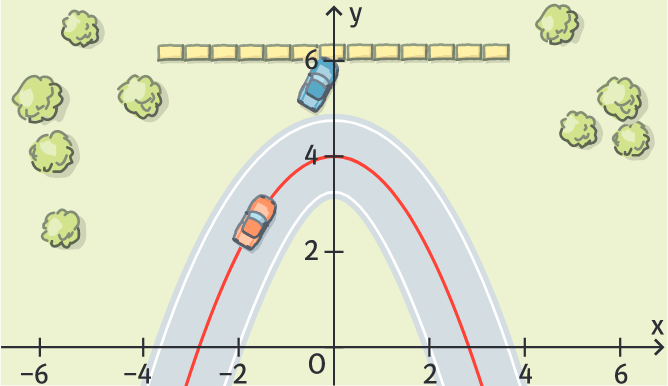
\includegraphics[width=0.5\textwidth]{/home/daniel/documents/docs/LaTeX/notes/math-figures/rennstrecke.png}
  \end{center}
\end{figure}

Die in der Abbildung rot gezeichnete Ideallinie einer Rennstrecke wird durch
die Funktion f mit 
\[ f(x)=4-\frac{1}{2}x^2\]
beschrieben. Die Strohballen werden durch die Gerade $y=6$ beschrieben.
Aufgrund eines Fahrfehlers kommt ein Rennwagen im Punkt $(-1|f(-1))$ von der
Ideallinie ab und trifft im Punkt Y auf die Strohballen.

\paragraph{Aufgabe 1} \textit{Bestimmen sie den Punkt Y zeichnerisch mithilfe der Abblidung. Beschreiben sie ihr vorgehen.}
Hier zu zeichnen ist offensichtlich unnoetig, man zeichnet die Tangente auf (-1|f(-1)), und schaut wo auf y=6 eintrifft.


\paragraph{Aufgabe 2} \textit{Berechnen Sie den Punkt Y.}

\begin{multicols}{2}

  \begin{enumerate}
    \item hoehe von f(-1) finden, also 
      \begin{align*}
        f(-1)&=4-\frac{1}{2}-1^2\\
        &=3,5\\
      \end{align*}
    \item nun die Ableitung um Steigung der Tangente zu haben.
      \begin{align*}
        f(x)&=4-\frac{1}{2}x^2\\
        f'(x)&=-x\\
             &\text{fuer $-1$ ist es dann $m=1$}\\
      \end{align*}
    \item daraus kann man eine Tangente machen
      \[y-y_1=m(x-x_1)\]
      hier ist $x=-1$, $y=3,5$ und steigung $m=1$. wenn man das einsetzt bekommt man:
      \[y-3,5=1(x+1)\]
      durch umformen erhaelt man $y=x+4,5$.
    \item um dann zu schauen wann diese $y=6$ erricht setzt man es in die
      gleichung ein: $6=x+4.5$ und duch loesen erhaelt man $x=0,5$
  \end{enumerate}
  \paragraph{Loesung:} nun sieht man das der Rennwagen auf $(1,5|6)$ einschlaegt.
\end{multicols}



\begin{tcolorbox}[colback=blue!10!white,colframe=blue!50!black,title=Tangentengleichung]
  Wir suchen die Gleichung der Tangente t an den Graphen einer Funktion f im Ber\"uhrpunkt $B(x_0|f(x_0))$.
  \[t:y=mx+c\]
  Steigung $f=f'(x_0)$
  \[\implies t:y=f'(x_0)x+c\]
  punkprobe mit B:
  \begin{align*}
    f(x_0)&=f'(x_0)\cdot x_0+c\\
    \Leftrightarrow c&=f(x_0)-f'(x_0)\cdot x_0\\
    \implies t:y&=f'(x_0)\cdot x+f(x_0)-f'(x_0)\cdot x_0\\
    \Leftrightarrow t: y=f'(x_0)\cdot (x-x_0)+f(x_0)
  \end{align*}
\end{tcolorbox}

\section{Arbeitsverbesserung}

\textbf{Besprechung der Klausur (Gruppenarbeit)}

\begin{enumerate}
  \item Besprechen Sie alle Aufgaben. Klären und korrigieren Sie dabei die
    Fehler jeder Schülerin bzw. jeden Schülers der Gruppe.
  \item Einigen Sie sich auf eine Musterlösung der Klausur. Achten Sie dabei
    auf Vollständigkeit, eine saubere Darstellung und korrekte Anwendung der
    Fachsprache. Die Musterlösung muss abgeben werden.
  \item Jeder Schüler soll in den kommenden Wochen an einer seiner
    Schwierigkeiten arbeiten. Besprechen Sie in der Gruppe, an welcher
    Schwierigkeit jede Schülerinbzw. jeder Schüler arbeiten wird.
\end{enumerate}

Reflexion der Klausur (Einzelarbeit)Beantworten Sie ehrlich folgende Fragen.

\begin{itemize}
  \item Ich bin mit dem Ergebnis der Klausur zufrieden. 
    \subitem \textit{Nein, Joa, Ja}

  \item Was haben Sie in der in der Klausur leicht lösen können? Was hat Ihnen
    Schwierigkeiten bereitet?
    \subitem \textit{Ableitungen waren eine Schwierigkeit, auch extremwerte und punkte}

  \item Wie haben Sie sich zu Hause auf die Klausur vorbereitet?
    \subitem Die Aufschriebe im Heft noch einmal durchgelesen. \textit{Ja, Joa, Nein}
    \subitem Grundbegriffe wiederholt. \textit{Nein, nicht so, Ja}
    \subitem Übungsaufgaben gelöst. \textit{Ja, ne, Nein}
    \subitem Andersweitig ge\"ubt Wie? \textit{Ja, Ne, Ja}

  \item Wie lange haben Sie für die Klausur gelernt? \textit{10h, 0.5h, 1h}

  \item Haben Sie aktiv im Unterricht mitgearbeitet? (ständig / häufig / wenig / nie) \textit{Nein, Ja, Nein}
    \subitem Im Unterrichtsgespräch? \textit{N\"o, wenig, ne}
    \subitem In den Arbeitsphasen? \textit{Joa, Ja schon, ein wenig}

  \item Was hätten Sie im Vorfeld der Klausur anders machen können, um Ihre Note zu verbessern?
    \subitem \textit{Weis ich nicht, mehr \"ubungsaufgaben, sich \"uberzeugen das es die Zeit wert ist}

  \item An welcher Schwierigkeit werden Sie in den kommenden Wochen arbeiten?
    \subitem \textit{Alles anders, Hausaufgaben machen, weniger Linux mehr rechnen}
\end{itemize}


\begin{multicols}{2}

\section{}
\subsection{}
\begin{align*}
  f(x)&=2x^3-\sqrt{5}\cdot x^2+9\\
  f'(x)&=6x^2-\sqrt{5}\cdot 2x-1\\
\end{align*}

\subsection{}
\begin{align*}
  u(t)&=-3\sqrt{t}+\frac{1}{t}\\
  u'(t)&=-\frac{3}{2}t^{-\frac{1}{2}}-t^{-2}\\
\end{align*}

\subsection{}
\begin{align*}
  g(x)&=4x^2\cdot e^{3x-2}\\
  g'(x)&=8xe^{3x-2}+12x^2\cdot e^{3x-2}\\
\end{align*}

\subsection{}

\begin{align*}
  h(x)&=cos(-x+6)\cdot sin(x)\\
  h'(x)&=\sin(-x+6)\cdot \sin(x) + \cos(-x +6) \cdot \cos(x)\\
\end{align*}

\section{}
\subsection{}
Wendepunkte: 1(0,5;0,5), 2(-0,5;0,5)

\section{}
\subsection{}
Falsch, grafisch kann man pruefen, dass die Ableitung $g'$ bei $x_0=1$ ungefaer
1 ist, in dem intervall $[3;6]$ die mittlere aenderungsrate aber nur $~
\frac{1}{2}$, also um die haelfte weniger.

\subsection{}
Wahr, da es in deiesem Bereich keine positive Steigung gibt.
\end{multicols}

\section*{Teil 2, Aufgabe 1}
\begin{align*}
  f'(x)&=\lim_{h\to 0}\frac{f(x+h)-f(x)}{h}\\
       &=\lim_{h\to 0}\frac{(-(x+h)^2+4(x+h)+3)-(-x^2+4x+3)}{h}\\
       &=\lim_{h\to 0}\frac{-x^2-2xh-h^2+4x+4h+3+x^2-4x-3}{h}\\
       &=\lim_{h\to 0}\frac{-2xh-h^2+4h}{h}\\
       &=\lim_{h\to 0}(-2x-h+4)\\
       &=-2x+4\\
\end{align*}
Daher ist die Ableitungsfunktion von $f(x)$ gleich $f'(x)=-2x+4$.

\section*{Aufgabe 2}

Gegeben ist die Funktion $h(x) = 5x^2 \cdot e^{\frac{2}{3} x^3}$ für $-2 \leq x
\leq 2$. Wir sollen zeigen, dass $h'(x) = 10x \cdot (1+x^3) \cdot
e^{\frac{2}{3} x^3}$ eine Gleichung der ersten Ableitung von $h$ ist.

Zunächst berechnen wir die Ableitung $h'(x)$ von $h(x)$ nach der Produktregel
und der Kettenregel:

\begin{align*}
h'(x) &= \frac{d}{dx}(5x^2) \cdot e^{\frac{2}{3} x^3} + 5x^2 \cdot \frac{d}{dx}(e^{\frac{2}{3} x^3})\\
      &= 10x \cdot e^{\frac{2}{3} x^3} + 5x^2 \cdot \frac{2}{3} x^2 \cdot e^{\frac{2}{3} x^3}\\
      &= 10x \cdot e^{\frac{2}{3} x^3} + 10x^3 \cdot e^{\frac{2}{3} x^3}
\end{align*}

Dann faktorisieren wir den Term $h'(x)$ mit $10x$:
\begin{align*}
  h'(x) &= 10x \cdot e^{\frac{2}{3} x^3} + 10x^3 \cdot e^{\frac{2}{3} x^3}\\
        &= 10x \cdot (1 + x^3) \cdot e^{\frac{2}{3} x^3}
\end{align*}
Daher ist $h'(x) = 10x \cdot (1+x^3) \cdot e^{\frac{2}{3} x^3}$ eine Gleichung
der ersten Ableitung von $h(x)$, wie gefordert.

\subsection*{2.2\&3}
Da die Funktion $h(x) = 5x^2 \cdot e^{\frac{2}{3} x^3}$ auf dem Intervall $-2
\leq x \leq 2$ stetig ist, existieren nach dem Satz von Weierstraß globale
Extremwerte auf diesem Intervall.

Um die globalen Extremwerte zu ermitteln, suchen wir zuerst die kritischen
Punkte von $h(x)$, d.h. die Punkte, an denen die Ableitung von $h(x)$ gleich
Null ist oder nicht existiert. Wir berechnen zuerst die erste Ableitung von
$h(x)$:

$h'(x) = 10x \cdot (1+x^3) \cdot e^{\frac{2}{3} x^3}$

$h'(x)$ ist genau dann gleich Null, wenn $x=0$ oder $x=-1$ oder $x=1$. Um zu
zeigen, dass $h'(x)$ für alle $x \in [-2,0)$ negativ und für alle $x \in (0,2]$
positiv ist, nutzen wir die Vorzeichenregel für Ableitungen:

Somit hat $h(x)$ bei $x=0$ ein lokales Maximum und bei $x=-1$ und $x=1$ jeweils
ein lokales Minimum auf dem Intervall $[-2,2]$. Da $h(x)$ für $x \rightarrow
-\infty$ und $x \rightarrow \infty$ gegen $0$ strebt, sind das globale Maximum
von $h(x)$ bei $x=0$ und das globale Minimum von $h(x)$ bei $x=-1$ und $x=1$.

Daher sind die globalen Extremwerte von $h(x)$ auf dem Intervall $[-2,2]$:
\begin{itemize}
  \item globales Maximum: $h(0) = 0$
  \item globales Minimum: $h(-1) = \frac{5}{e^{\frac{2}{3}}} \approx 0.7648$ und $h(1) = \frac{5}{e^{\frac{2}{3}}} \approx 0.7648$
\end{itemize}


\section{Abi Aufgaben}
\textit{auf papier gemacht}

\section{Integralrechnung, Rekonstruktion}
Die Gesamt\"anderung der gr\"ose kann man auis ihrem momnetaner \"Anderungsrate
rekonstruieren -- man sagt auch integrieren (integrare $\rightarrow$ wiederherstellen) --, 
indem man den orientierten Fl\"acheninhalt zwischen dem Graphen der momentanen \"Anderungsrate 
und der x-Achse bestimmt.


\subsection{Hausaufgaben}

We want to approximate the area under the curve $y=-x^2+4$ from $x=-2$ to $x=2$
using the Riemann sum method.

Let's divide the interval $[-2,2]$ into $n$ subintervals of equal width $\Delta
x$, where $\Delta x = \frac{4}{n}$.

For each subinterval $i$, where $i=0,1,\dots,n-1$, we choose a point $x_i$ in
the interval $[x_i,x_{i+1}]$, where $x_i = -2 + i\Delta x$ and $x_{i+1} = x_i +
\Delta x$.

The area of each rectangle with base $\Delta x$ and height $f(x_i) = -x_i^2+4$
is given by $\Delta x \cdot f(x_i)$. Thus, the Riemann sum approximation of the
area under the curve is

\[A_n = \sum_{i=0}^{n-1} \Delta x \cdot f(x_i) = \sum_{i=0}^{n-1} \frac{4}{n}
\cdot \left(-\left(-2 + i\frac{4}{n}\right)^2 + 4\right)\]

We can use this formula to calculate the approximation for any value of $n$.
For example, let's calculate $A_5$:

\[
A_5 = \frac{4}{5}\left(f(-2) + f(-1.2) + f(-0.4) + f(0.4) + f(1.2)\right) \approx 8.64
\]

\begin{tikzpicture}
\begin{axis}[
    xlabel=$x$,
    ylabel=$y$,
    domain=-2:2,
    samples=100,
    axis lines=middle,
    xtick={-2,-1,0,1,2},
    ytick={0,1,2,3,4},
    xmin=-2.2,
    xmax=2.2,
    ymin=-0.2,
    ymax=4.2,
]
\pgfplotsinvokeforeach{-1.6,-1.2,...,1.6}{
    \draw[fill=gray!50] (#1,0) rectangle (#1+0.4,{-(#1+0.2)^2+4});
}
\addplot[blue, thick] {-x^2+4};
\end{axis}
\end{tikzpicture}




\end{document}
